% Options for packages loaded elsewhere
\PassOptionsToPackage{unicode}{hyperref}
\PassOptionsToPackage{hyphens}{url}
\PassOptionsToPackage{dvipsnames,svgnames,x11names}{xcolor}
%
\documentclass[
  a4paper,
  DIV=11,
  numbers=noendperiod]{scrreprt}

\usepackage{amsmath,amssymb}
\usepackage{iftex}
\ifPDFTeX
  \usepackage[T1]{fontenc}
  \usepackage[utf8]{inputenc}
  \usepackage{textcomp} % provide euro and other symbols
\else % if luatex or xetex
  \usepackage{unicode-math}
  \defaultfontfeatures{Scale=MatchLowercase}
  \defaultfontfeatures[\rmfamily]{Ligatures=TeX,Scale=1}
\fi
\usepackage{lmodern}
\ifPDFTeX\else  
    % xetex/luatex font selection
\fi
% Use upquote if available, for straight quotes in verbatim environments
\IfFileExists{upquote.sty}{\usepackage{upquote}}{}
\IfFileExists{microtype.sty}{% use microtype if available
  \usepackage[]{microtype}
  \UseMicrotypeSet[protrusion]{basicmath} % disable protrusion for tt fonts
}{}
\makeatletter
\@ifundefined{KOMAClassName}{% if non-KOMA class
  \IfFileExists{parskip.sty}{%
    \usepackage{parskip}
  }{% else
    \setlength{\parindent}{0pt}
    \setlength{\parskip}{6pt plus 2pt minus 1pt}}
}{% if KOMA class
  \KOMAoptions{parskip=half}}
\makeatother
\usepackage{xcolor}
\usepackage[lmargin=10mm,rmargin=10mm,tmargin=15mm,bmargin=15mm]{geometry}
\setlength{\emergencystretch}{3em} % prevent overfull lines
\setcounter{secnumdepth}{5}
% Make \paragraph and \subparagraph free-standing
\ifx\paragraph\undefined\else
  \let\oldparagraph\paragraph
  \renewcommand{\paragraph}[1]{\oldparagraph{#1}\mbox{}}
\fi
\ifx\subparagraph\undefined\else
  \let\oldsubparagraph\subparagraph
  \renewcommand{\subparagraph}[1]{\oldsubparagraph{#1}\mbox{}}
\fi

\usepackage{color}
\usepackage{fancyvrb}
\newcommand{\VerbBar}{|}
\newcommand{\VERB}{\Verb[commandchars=\\\{\}]}
\DefineVerbatimEnvironment{Highlighting}{Verbatim}{commandchars=\\\{\}}
% Add ',fontsize=\small' for more characters per line
\usepackage{framed}
\definecolor{shadecolor}{RGB}{241,243,245}
\newenvironment{Shaded}{\begin{snugshade}}{\end{snugshade}}
\newcommand{\AlertTok}[1]{\textcolor[rgb]{0.68,0.00,0.00}{#1}}
\newcommand{\AnnotationTok}[1]{\textcolor[rgb]{0.37,0.37,0.37}{#1}}
\newcommand{\AttributeTok}[1]{\textcolor[rgb]{0.40,0.45,0.13}{#1}}
\newcommand{\BaseNTok}[1]{\textcolor[rgb]{0.68,0.00,0.00}{#1}}
\newcommand{\BuiltInTok}[1]{\textcolor[rgb]{0.00,0.23,0.31}{#1}}
\newcommand{\CharTok}[1]{\textcolor[rgb]{0.13,0.47,0.30}{#1}}
\newcommand{\CommentTok}[1]{\textcolor[rgb]{0.37,0.37,0.37}{#1}}
\newcommand{\CommentVarTok}[1]{\textcolor[rgb]{0.37,0.37,0.37}{\textit{#1}}}
\newcommand{\ConstantTok}[1]{\textcolor[rgb]{0.56,0.35,0.01}{#1}}
\newcommand{\ControlFlowTok}[1]{\textcolor[rgb]{0.00,0.23,0.31}{#1}}
\newcommand{\DataTypeTok}[1]{\textcolor[rgb]{0.68,0.00,0.00}{#1}}
\newcommand{\DecValTok}[1]{\textcolor[rgb]{0.68,0.00,0.00}{#1}}
\newcommand{\DocumentationTok}[1]{\textcolor[rgb]{0.37,0.37,0.37}{\textit{#1}}}
\newcommand{\ErrorTok}[1]{\textcolor[rgb]{0.68,0.00,0.00}{#1}}
\newcommand{\ExtensionTok}[1]{\textcolor[rgb]{0.00,0.23,0.31}{#1}}
\newcommand{\FloatTok}[1]{\textcolor[rgb]{0.68,0.00,0.00}{#1}}
\newcommand{\FunctionTok}[1]{\textcolor[rgb]{0.28,0.35,0.67}{#1}}
\newcommand{\ImportTok}[1]{\textcolor[rgb]{0.00,0.46,0.62}{#1}}
\newcommand{\InformationTok}[1]{\textcolor[rgb]{0.37,0.37,0.37}{#1}}
\newcommand{\KeywordTok}[1]{\textcolor[rgb]{0.00,0.23,0.31}{#1}}
\newcommand{\NormalTok}[1]{\textcolor[rgb]{0.00,0.23,0.31}{#1}}
\newcommand{\OperatorTok}[1]{\textcolor[rgb]{0.37,0.37,0.37}{#1}}
\newcommand{\OtherTok}[1]{\textcolor[rgb]{0.00,0.23,0.31}{#1}}
\newcommand{\PreprocessorTok}[1]{\textcolor[rgb]{0.68,0.00,0.00}{#1}}
\newcommand{\RegionMarkerTok}[1]{\textcolor[rgb]{0.00,0.23,0.31}{#1}}
\newcommand{\SpecialCharTok}[1]{\textcolor[rgb]{0.37,0.37,0.37}{#1}}
\newcommand{\SpecialStringTok}[1]{\textcolor[rgb]{0.13,0.47,0.30}{#1}}
\newcommand{\StringTok}[1]{\textcolor[rgb]{0.13,0.47,0.30}{#1}}
\newcommand{\VariableTok}[1]{\textcolor[rgb]{0.07,0.07,0.07}{#1}}
\newcommand{\VerbatimStringTok}[1]{\textcolor[rgb]{0.13,0.47,0.30}{#1}}
\newcommand{\WarningTok}[1]{\textcolor[rgb]{0.37,0.37,0.37}{\textit{#1}}}

\providecommand{\tightlist}{%
  \setlength{\itemsep}{0pt}\setlength{\parskip}{0pt}}\usepackage{longtable,booktabs,array}
\usepackage{calc} % for calculating minipage widths
% Correct order of tables after \paragraph or \subparagraph
\usepackage{etoolbox}
\makeatletter
\patchcmd\longtable{\par}{\if@noskipsec\mbox{}\fi\par}{}{}
\makeatother
% Allow footnotes in longtable head/foot
\IfFileExists{footnotehyper.sty}{\usepackage{footnotehyper}}{\usepackage{footnote}}
\makesavenoteenv{longtable}
\usepackage{graphicx}
\makeatletter
\def\maxwidth{\ifdim\Gin@nat@width>\linewidth\linewidth\else\Gin@nat@width\fi}
\def\maxheight{\ifdim\Gin@nat@height>\textheight\textheight\else\Gin@nat@height\fi}
\makeatother
% Scale images if necessary, so that they will not overflow the page
% margins by default, and it is still possible to overwrite the defaults
% using explicit options in \includegraphics[width, height, ...]{}
\setkeys{Gin}{width=\maxwidth,height=\maxheight,keepaspectratio}
% Set default figure placement to htbp
\makeatletter
\def\fps@figure{htbp}
\makeatother

\usepackage[hangul]{kotex}
\usepackage{iftex}
\ifPDFTeX
 \usepackage{dhucs-nanumfont}
\else\ifXeTeX
 \setmainhangulfont{NanumMyeongjo}
\else\ifLuaTeX
 \setmainhangulfont{NanumMyeongjo}
\fi\fi\fi
\KOMAoption{captions}{tableheading}
\makeatletter
\@ifpackageloaded{tcolorbox}{}{\usepackage[skins,breakable]{tcolorbox}}
\@ifpackageloaded{fontawesome5}{}{\usepackage{fontawesome5}}
\definecolor{quarto-callout-color}{HTML}{909090}
\definecolor{quarto-callout-note-color}{HTML}{0758E5}
\definecolor{quarto-callout-important-color}{HTML}{CC1914}
\definecolor{quarto-callout-warning-color}{HTML}{EB9113}
\definecolor{quarto-callout-tip-color}{HTML}{00A047}
\definecolor{quarto-callout-caution-color}{HTML}{FC5300}
\definecolor{quarto-callout-color-frame}{HTML}{acacac}
\definecolor{quarto-callout-note-color-frame}{HTML}{4582ec}
\definecolor{quarto-callout-important-color-frame}{HTML}{d9534f}
\definecolor{quarto-callout-warning-color-frame}{HTML}{f0ad4e}
\definecolor{quarto-callout-tip-color-frame}{HTML}{02b875}
\definecolor{quarto-callout-caution-color-frame}{HTML}{fd7e14}
\makeatother
\makeatletter
\@ifpackageloaded{bookmark}{}{\usepackage{bookmark}}
\makeatother
\makeatletter
\@ifpackageloaded{caption}{}{\usepackage{caption}}
\AtBeginDocument{%
\ifdefined\contentsname
  \renewcommand*\contentsname{Table of contents}
\else
  \newcommand\contentsname{Table of contents}
\fi
\ifdefined\listfigurename
  \renewcommand*\listfigurename{List of Figures}
\else
  \newcommand\listfigurename{List of Figures}
\fi
\ifdefined\listtablename
  \renewcommand*\listtablename{List of Tables}
\else
  \newcommand\listtablename{List of Tables}
\fi
\ifdefined\figurename
  \renewcommand*\figurename{Figure}
\else
  \newcommand\figurename{Figure}
\fi
\ifdefined\tablename
  \renewcommand*\tablename{Table}
\else
  \newcommand\tablename{Table}
\fi
}
\@ifpackageloaded{float}{}{\usepackage{float}}
\floatstyle{ruled}
\@ifundefined{c@chapter}{\newfloat{codelisting}{h}{lop}}{\newfloat{codelisting}{h}{lop}[chapter]}
\floatname{codelisting}{Listing}
\newcommand*\listoflistings{\listof{codelisting}{List of Listings}}
\makeatother
\makeatletter
\makeatother
\makeatletter
\@ifpackageloaded{caption}{}{\usepackage{caption}}
\@ifpackageloaded{subcaption}{}{\usepackage{subcaption}}
\makeatother
\makeatletter
\@ifpackageloaded{tcolorbox}{}{\usepackage[skins,breakable]{tcolorbox}}
\makeatother
\makeatletter
\@ifundefined{shadecolor}{\definecolor{shadecolor}{HTML}{31BAE9}}{}
\makeatother
\makeatletter
\makeatother
\makeatletter
\ifdefined\Shaded\renewenvironment{Shaded}{\begin{tcolorbox}[boxrule=0pt, interior hidden, frame hidden, enhanced, sharp corners, breakable, borderline west={3pt}{0pt}{shadecolor}]}{\end{tcolorbox}}\fi
\makeatother
\ifLuaTeX
  \usepackage{selnolig}  % disable illegal ligatures
\fi
\usepackage{bookmark}

\IfFileExists{xurl.sty}{\usepackage{xurl}}{} % add URL line breaks if available
\urlstyle{same} % disable monospaced font for URLs
\hypersetup{
  pdftitle={KAIST MFE, 2024 Spring},
  pdfauthor={Kim Hyeonghwan},
  colorlinks=true,
  linkcolor={blue},
  filecolor={Maroon},
  citecolor={Blue},
  urlcolor={Blue},
  pdfcreator={LaTeX via pandoc}}

\title{KAIST MFE, 2024 Spring}
\author{Kim Hyeonghwan}
\date{2024-04-29}

\begin{document}
\maketitle

\renewcommand*\contentsname{Table of contents}
{
\hypersetup{linkcolor=}
\setcounter{tocdepth}{2}
\tableofcontents
}
\bookmarksetup{startatroot}

\chapter*{Welcome!}\label{welcome}
\addcontentsline{toc}{chapter}{Welcome!}

\markboth{Welcome!}{Welcome!}

안녕하세요, KAIST MFE 24년 봄학기에 이수한 과목의 과제 등을
정리해두었습니다.

\part{Python('24봄)}

\chapter{Python Basics}\label{python-basics}

\section{Values and Variables}\label{values-and-variables}

\subsection{- Values}\label{values}

\begin{Shaded}
\begin{Highlighting}[]
\BuiltInTok{type}\NormalTok{(}\StringTok{"Hello, World"}\NormalTok{)}
\end{Highlighting}
\end{Shaded}

\begin{verbatim}
str
\end{verbatim}

\begin{Shaded}
\begin{Highlighting}[]
\BuiltInTok{type}\NormalTok{(())}
\end{Highlighting}
\end{Shaded}

\begin{verbatim}
tuple
\end{verbatim}

\begin{Shaded}
\begin{Highlighting}[]
\BuiltInTok{type}\NormalTok{([])}
\end{Highlighting}
\end{Shaded}

\begin{verbatim}
list
\end{verbatim}

\begin{Shaded}
\begin{Highlighting}[]
\BuiltInTok{type}\NormalTok{(}\BuiltInTok{set}\NormalTok{())}
\end{Highlighting}
\end{Shaded}

\begin{verbatim}
set
\end{verbatim}

\begin{Shaded}
\begin{Highlighting}[]
\BuiltInTok{type}\NormalTok{(\{\})}
\end{Highlighting}
\end{Shaded}

\begin{verbatim}
dict
\end{verbatim}

\begin{Shaded}
\begin{Highlighting}[]
\CommentTok{\# 파이썬에서는 복소수 i를 j로 표현함}
\BuiltInTok{type}\NormalTok{(}\DecValTok{2}\OperatorTok{+}\OtherTok{3j}\NormalTok{)}
\end{Highlighting}
\end{Shaded}

\begin{verbatim}
complex
\end{verbatim}

\subsection{- Variables}\label{variables}

\begin{Shaded}
\begin{Highlighting}[]
\NormalTok{message}\OperatorTok{=}\StringTok{"Hello, world!"}
\NormalTok{n}\OperatorTok{=}\DecValTok{42}
\NormalTok{e}\OperatorTok{=}\FloatTok{2.71}
\BuiltInTok{print}\NormalTok{(n)}
\BuiltInTok{print}\NormalTok{(message)}
\end{Highlighting}
\end{Shaded}

\begin{verbatim}
42
Hello, world!
\end{verbatim}

\begin{Shaded}
\begin{Highlighting}[]
\NormalTok{length}\OperatorTok{=}\FloatTok{4.2}
\NormalTok{height}\OperatorTok{=}\FloatTok{3.5}
\NormalTok{area}\OperatorTok{=}\NormalTok{length}\OperatorTok{*}\NormalTok{height}
\BuiltInTok{print}\NormalTok{(area)}
\end{Highlighting}
\end{Shaded}

\begin{verbatim}
14.700000000000001
\end{verbatim}

\begin{Shaded}
\begin{Highlighting}[]
\CommentTok{\# 변수는 방문앞에 이름만 바꾼것... 새로운 변수에 기존 변수를 할당하고, 기존 변수를 변경하면 새로운 변수도 영향받음}
\NormalTok{a}\OperatorTok{=}\NormalTok{[}\DecValTok{1}\NormalTok{,}\DecValTok{2}\NormalTok{,}\DecValTok{3}\NormalTok{]}
\NormalTok{b}\OperatorTok{=}\NormalTok{a}
\NormalTok{a[}\DecValTok{0}\NormalTok{]}\OperatorTok{=}\DecValTok{10}
\BuiltInTok{print}\NormalTok{(b)}
\end{Highlighting}
\end{Shaded}

\begin{verbatim}
[10, 2, 3]
\end{verbatim}

\subsection{- Variable names}\label{variable-names}

\begin{itemize}
\tightlist
\item
  숫자로 시작하면 안됌
\end{itemize}

\begin{Shaded}
\begin{Highlighting}[]
\NormalTok{x}\OperatorTok{=}\FloatTok{1.0}
\NormalTok{X}\OperatorTok{=}\FloatTok{1.0}
\NormalTok{X1}\OperatorTok{=}\FloatTok{1.0}
\NormalTok{x1}\OperatorTok{=}\FloatTok{1.0}
\NormalTok{dell}\OperatorTok{=}\FloatTok{1.0}
\CommentTok{\# not allowed}
\CommentTok{\# x:, 1X, X1{-}1, for}
\end{Highlighting}
\end{Shaded}

\begin{Shaded}
\begin{Highlighting}[]
\NormalTok{x,y,z}\OperatorTok{=}\DecValTok{1}\NormalTok{,}\FloatTok{3.14}\NormalTok{,}\StringTok{\textquotesingle{}a\textquotesingle{}}
\BuiltInTok{print}\NormalTok{(x,y,z)}
\end{Highlighting}
\end{Shaded}

\begin{verbatim}
1 3.14 a
\end{verbatim}

\section{Core Data Types}\label{core-data-types}

\subsection{- Floating Point(float)}\label{floating-pointfloat}

\begin{Shaded}
\begin{Highlighting}[]
\NormalTok{x}\OperatorTok{=}\DecValTok{1}
\NormalTok{y}\OperatorTok{=}\FloatTok{1.0}
\NormalTok{z}\OperatorTok{=}\BuiltInTok{float}\NormalTok{(}\DecValTok{1}\NormalTok{)}
\NormalTok{xx}\OperatorTok{=}\FloatTok{1.234e{-}5}
\BuiltInTok{print}\NormalTok{(x,y,z,xx)}
\BuiltInTok{print}\NormalTok{(}\BuiltInTok{type}\NormalTok{(z),}\BuiltInTok{type}\NormalTok{(}\BuiltInTok{float}\NormalTok{(}\VariableTok{True}\NormalTok{)))}
\end{Highlighting}
\end{Shaded}

\begin{verbatim}
1 1.0 1.0 1.234e-05
<class 'float'> <class 'float'>
\end{verbatim}

\begin{Shaded}
\begin{Highlighting}[]
\CommentTok{\# float 타입은 근사치를 사용하기때문에 사용에 유의}
\DecValTok{1}\OperatorTok{{-}}\FloatTok{0.9}\OperatorTok{==}\FloatTok{0.1}
\end{Highlighting}
\end{Shaded}

\begin{verbatim}
False
\end{verbatim}

\begin{Shaded}
\begin{Highlighting}[]
\BuiltInTok{float}\NormalTok{(}\StringTok{\textquotesingle{}inf\textquotesingle{}}\NormalTok{)}
\end{Highlighting}
\end{Shaded}

\begin{verbatim}
inf
\end{verbatim}

\subsection{- Complex}\label{complex}

\begin{Shaded}
\begin{Highlighting}[]
\NormalTok{x}\OperatorTok{=}\OtherTok{1j}
\NormalTok{y}\OperatorTok{=}\DecValTok{2}\OperatorTok{+}\OtherTok{3j}
\NormalTok{z}\OperatorTok{=}\BuiltInTok{complex}\NormalTok{(}\DecValTok{1}\NormalTok{)}
\BuiltInTok{print}\NormalTok{(x,y,z,y.real,y.imag)}
\BuiltInTok{print}\NormalTok{(}\BuiltInTok{type}\NormalTok{(y.imag))}
\end{Highlighting}
\end{Shaded}

\begin{verbatim}
1j (2+3j) (1+0j) 2.0 3.0
<class 'float'>
\end{verbatim}

\subsection{- Integer}\label{integer}

\begin{Shaded}
\begin{Highlighting}[]
\CommentTok{\# Integer는 float와 달리 정확하다}
\NormalTok{x}\OperatorTok{=}\DecValTok{2}\OperatorTok{**}\DecValTok{127}\OperatorTok{+}\DecValTok{2}\OperatorTok{**}\DecValTok{65} 
\NormalTok{x}
\end{Highlighting}
\end{Shaded}

\begin{verbatim}
170141183460469231768580791863303208960
\end{verbatim}

\subsection{- Boolean(bool)}\label{booleanbool}

\begin{Shaded}
\begin{Highlighting}[]
\BuiltInTok{print}\NormalTok{(}\BuiltInTok{bool}\NormalTok{(}\DecValTok{1}\NormalTok{),}\BuiltInTok{bool}\NormalTok{(}\FloatTok{1.2}\NormalTok{),}\BuiltInTok{bool}\NormalTok{(}\OperatorTok{{-}}\DecValTok{1}\NormalTok{),}\BuiltInTok{bool}\NormalTok{(}\FloatTok{0.1}\NormalTok{))}
\end{Highlighting}
\end{Shaded}

\begin{verbatim}
True True True True
\end{verbatim}

\begin{Shaded}
\begin{Highlighting}[]
\BuiltInTok{print}\NormalTok{(}\BuiltInTok{bool}\NormalTok{(}\DecValTok{0}\NormalTok{),}\BuiltInTok{bool}\NormalTok{(}\FloatTok{0.0}\NormalTok{),}\BuiltInTok{bool}\NormalTok{(}\FloatTok{0.0000}\NormalTok{),}\BuiltInTok{bool}\NormalTok{(}\VariableTok{None}\NormalTok{),}\BuiltInTok{bool}\NormalTok{(}\StringTok{""}\NormalTok{),}\BuiltInTok{bool}\NormalTok{(()))}
\end{Highlighting}
\end{Shaded}

\begin{verbatim}
False False False False False False
\end{verbatim}

\begin{Shaded}
\begin{Highlighting}[]
\DecValTok{3}\OperatorTok{\textgreater{}}\DecValTok{4}
\end{Highlighting}
\end{Shaded}

\begin{verbatim}
False
\end{verbatim}

\section{Operators}\label{operators}

\subsection{- Arithmetic Operators}\label{arithmetic-operators}

\begin{Shaded}
\begin{Highlighting}[]
\NormalTok{a}\OperatorTok{=}\DecValTok{10}
\NormalTok{b}\OperatorTok{=}\DecValTok{20}
\end{Highlighting}
\end{Shaded}

\begin{Shaded}
\begin{Highlighting}[]
\CommentTok{\# 나누기 연산은 항상 float로 반환됨을 유의}
\BuiltInTok{print}\NormalTok{(a}\OperatorTok{+}\NormalTok{b,a}\OperatorTok{{-}}\NormalTok{b,a}\OperatorTok{*}\NormalTok{b,b}\OperatorTok{/}\NormalTok{a)}
\end{Highlighting}
\end{Shaded}

\begin{verbatim}
30 -10 200 2.0
\end{verbatim}

\begin{Shaded}
\begin{Highlighting}[]
\CommentTok{\# 나머지 연산자}
\NormalTok{b}\OperatorTok{\%}\NormalTok{a}
\end{Highlighting}
\end{Shaded}

\begin{verbatim}
0
\end{verbatim}

\begin{Shaded}
\begin{Highlighting}[]
\CommentTok{\# 몫 연산자}
\NormalTok{b}\OperatorTok{//}\NormalTok{a}
\end{Highlighting}
\end{Shaded}

\begin{verbatim}
2
\end{verbatim}

\begin{Shaded}
\begin{Highlighting}[]
\CommentTok{\# 거듭제곱 연산자, 우선순위가 가장 높음}
\NormalTok{a}\OperatorTok{**}\NormalTok{b}
\end{Highlighting}
\end{Shaded}

\begin{verbatim}
100000000000000000000
\end{verbatim}

\subsection{- Relational Operators}\label{relational-operators}

\begin{Shaded}
\begin{Highlighting}[]
\BuiltInTok{print}\NormalTok{(a}\OperatorTok{==}\NormalTok{b,a}\OperatorTok{!=}\NormalTok{b,a}\OperatorTok{\textgreater{}}\NormalTok{b,a}\OperatorTok{\textless{}}\NormalTok{b,a}\OperatorTok{\textgreater{}=}\NormalTok{b,a}\OperatorTok{\textless{}=}\NormalTok{b)}
\end{Highlighting}
\end{Shaded}

\begin{verbatim}
False True False True False True
\end{verbatim}

\subsection{- Assignment Operators}\label{assignment-operators}

\begin{Shaded}
\begin{Highlighting}[]
\NormalTok{t}\OperatorTok{=}\DecValTok{0}
\NormalTok{t}\OperatorTok{+=}\DecValTok{1}
\NormalTok{t}
\end{Highlighting}
\end{Shaded}

\begin{verbatim}
1
\end{verbatim}

\begin{Shaded}
\begin{Highlighting}[]
\NormalTok{t}\OperatorTok{/=}\DecValTok{2}
\NormalTok{t}
\end{Highlighting}
\end{Shaded}

\begin{verbatim}
0.5
\end{verbatim}

\begin{Shaded}
\begin{Highlighting}[]
\NormalTok{t}\OperatorTok{*=}\DecValTok{2}
\NormalTok{t}
\end{Highlighting}
\end{Shaded}

\begin{verbatim}
1.0
\end{verbatim}

\subsection{- Logical Operators}\label{logical-operators}

\begin{Shaded}
\begin{Highlighting}[]
\BuiltInTok{print}\NormalTok{(}\VariableTok{True} \KeywordTok{and} \VariableTok{False}\NormalTok{, }\VariableTok{True} \KeywordTok{or} \VariableTok{False}\NormalTok{, }\KeywordTok{not} \VariableTok{True}\NormalTok{)}
\end{Highlighting}
\end{Shaded}

\begin{verbatim}
False True False
\end{verbatim}

\begin{Shaded}
\begin{Highlighting}[]
\CommentTok{\# 논리연산자는 container가 bool이 아닌 경우 용법이 다름}
\CommentTok{\# or은 가장 먼저나오는 True값을 반환, and는 가장 먼저나오는 false값을 반환}
\BuiltInTok{print}\NormalTok{(}\StringTok{\textquotesingle{}\textquotesingle{}} \KeywordTok{or} \StringTok{\textquotesingle{}abc\textquotesingle{}}\NormalTok{,}\DecValTok{0} \KeywordTok{or} \DecValTok{1}\NormalTok{, }\StringTok{\textquotesingle{}abc\textquotesingle{}} \KeywordTok{or} \StringTok{\textquotesingle{}\textquotesingle{}}\NormalTok{,}\StringTok{\textquotesingle{}abc\textquotesingle{}} \KeywordTok{or} \StringTok{\textquotesingle{}ab\textquotesingle{}}\NormalTok{)}
\BuiltInTok{print}\NormalTok{(}\DecValTok{1} \KeywordTok{and} \DecValTok{0}\NormalTok{, }\StringTok{\textquotesingle{}abc\textquotesingle{}} \KeywordTok{and} \DecValTok{0}\NormalTok{, }\VariableTok{None} \KeywordTok{and} \StringTok{\textquotesingle{}\textquotesingle{}} \KeywordTok{and} \DecValTok{0}\NormalTok{)}
\end{Highlighting}
\end{Shaded}

\begin{verbatim}
abc 1 abc abc
0 0 None
\end{verbatim}

\section{Python Operators Precedence}\label{python-operators-precedence}

\subsection{- Python Operators
Precedence}\label{python-operators-precedence-1}

\begin{Shaded}
\begin{Highlighting}[]
\CommentTok{\# 거듭제곱 \textgreater{} 덧샘뺄샘 \textgreater{} 나눗셈, 몫, 나머지 \textgreater{} 부등호 \textgreater{} 논리}
\DecValTok{1}\OperatorTok{+}\DecValTok{3}\OperatorTok{/}\DecValTok{2}
\end{Highlighting}
\end{Shaded}

\begin{verbatim}
2.5
\end{verbatim}

\begin{Shaded}
\begin{Highlighting}[]
\DecValTok{2400}\OperatorTok{//}\DecValTok{500}\OperatorTok{*}\DecValTok{500}\OperatorTok{+}\DecValTok{2000}\OperatorTok{\%}\DecValTok{500}
\end{Highlighting}
\end{Shaded}

\begin{verbatim}
2000
\end{verbatim}

\begin{Shaded}
\begin{Highlighting}[]
\NormalTok{(}\DecValTok{2400}\OperatorTok{//}\DecValTok{500}\NormalTok{)}\OperatorTok{*}\DecValTok{500}\OperatorTok{+}\NormalTok{(}\DecValTok{2000}\OperatorTok{\%}\DecValTok{500}\NormalTok{)}
\end{Highlighting}
\end{Shaded}

\begin{verbatim}
2000
\end{verbatim}

\section{Mathmatical Function}\label{mathmatical-function}

\begin{Shaded}
\begin{Highlighting}[]
\CommentTok{\# built{-}in}
\BuiltInTok{print}\NormalTok{(}\BuiltInTok{abs}\NormalTok{(}\OperatorTok{{-}}\DecValTok{1}\NormalTok{),}\BuiltInTok{round}\NormalTok{(}\FloatTok{1.111}\NormalTok{,}\DecValTok{1}\NormalTok{))}
\end{Highlighting}
\end{Shaded}

\begin{verbatim}
1 1.1
\end{verbatim}

\begin{Shaded}
\begin{Highlighting}[]
\CommentTok{\# functional in math module}
\ImportTok{import}\NormalTok{ math}

\CommentTok{\# factorial, floor, isfinite, isinf, isnan, trunc}
\CommentTok{\# exp, log, log10, sqrt, cos, sin, tan, degrees, radians, pi, e}

\BuiltInTok{print}\NormalTok{(}
\NormalTok{math.ceil(}\FloatTok{1.11}\NormalTok{),}
\NormalTok{math.log(}\DecValTok{10}\NormalTok{),}
\NormalTok{math.log(}\DecValTok{10}\NormalTok{,}\DecValTok{10}\NormalTok{),}
\NormalTok{math.exp(}\DecValTok{1}\NormalTok{),}
\NormalTok{math.e,}
\NormalTok{math.pi,}
\NormalTok{math.trunc(math.pi),}
\NormalTok{math.degrees(}\DecValTok{1}\NormalTok{),}
\NormalTok{math.cos(math.pi)}
\NormalTok{)}
\end{Highlighting}
\end{Shaded}

\begin{verbatim}
2 2.302585092994046 1.0 2.718281828459045 2.718281828459045 3.141592653589793 3 57.29577951308232 -1.0
\end{verbatim}

\section{Python I/O}\label{python-io}

\subsection{- Python Output}\label{python-output}

\begin{Shaded}
\begin{Highlighting}[]
\CommentTok{\# print(object1, object2, ... , sep=\textquotesingle{} \textquotesingle{}, end=\textquotesingle{}\textbackslash{}n\textquotesingle{},...)}
\BuiltInTok{print}\NormalTok{(}\DecValTok{1}\NormalTok{,}\DecValTok{2}\NormalTok{,}\DecValTok{3}\NormalTok{,}\DecValTok{4}\NormalTok{)}
\BuiltInTok{print}\NormalTok{(}\DecValTok{1}\NormalTok{,}\DecValTok{2}\NormalTok{,}\DecValTok{3}\NormalTok{,}\DecValTok{4}\NormalTok{,sep}\OperatorTok{=}\StringTok{\textquotesingle{}*\textquotesingle{}}\NormalTok{)}
\BuiltInTok{print}\NormalTok{(}\DecValTok{1}\NormalTok{,}\DecValTok{2}\NormalTok{,}\DecValTok{3}\NormalTok{,}\DecValTok{4}\NormalTok{,end}\OperatorTok{=}\StringTok{\textquotesingle{}END\textquotesingle{}}\NormalTok{)}
\BuiltInTok{print}\NormalTok{(}\DecValTok{1}\NormalTok{,}\DecValTok{2}\NormalTok{,}\DecValTok{3}\NormalTok{,}\DecValTok{4}\NormalTok{,sep}\OperatorTok{=}\StringTok{\textquotesingle{}\textquotesingle{}}\NormalTok{)}
\end{Highlighting}
\end{Shaded}

\begin{verbatim}
1 2 3 4
1*2*3*4
1 2 3 4END1234
\end{verbatim}

\begin{Shaded}
\begin{Highlighting}[]
\CommentTok{\# formatting}
\NormalTok{x}\OperatorTok{=}\DecValTok{5}\OperatorTok{;}\NormalTok{ y}\OperatorTok{=}\DecValTok{10}
\BuiltInTok{print}\NormalTok{(}\StringTok{\textquotesingle{}The value of x is }\SpecialCharTok{\{\}}\StringTok{ and y is }\SpecialCharTok{\{\}}\StringTok{\textquotesingle{}}\NormalTok{.}\BuiltInTok{format}\NormalTok{(x,y))}
\BuiltInTok{print}\NormalTok{(}\StringTok{\textquotesingle{}I love }\SpecialCharTok{\{2\}}\StringTok{ and }\SpecialCharTok{\{1\}}\StringTok{, but hate }\SpecialCharTok{\{0\}}\StringTok{\textquotesingle{}}\NormalTok{.}\BuiltInTok{format}\NormalTok{(}\StringTok{\textquotesingle{}cucumber\textquotesingle{}}\NormalTok{,}\StringTok{\textquotesingle{}butter\textquotesingle{}}\NormalTok{,}\StringTok{\textquotesingle{}bread\textquotesingle{}}\NormalTok{))}
\end{Highlighting}
\end{Shaded}

\begin{verbatim}
The value of x is 5 and y is 10
I love bread and butter, but hate cucumber
\end{verbatim}

\subsection{- Python Input}\label{python-input}

\begin{Shaded}
\begin{Highlighting}[]
\CommentTok{\# Input value is a string}
\NormalTok{num}\OperatorTok{=}\BuiltInTok{input}\NormalTok{(}\StringTok{\textquotesingle{}Enter a number:\textquotesingle{}}\NormalTok{)}
\BuiltInTok{print}\NormalTok{(num)}
\BuiltInTok{print}\NormalTok{(}\BuiltInTok{int}\NormalTok{(num))}
\end{Highlighting}
\end{Shaded}

\begin{verbatim}
10
10
\end{verbatim}

\chapter{Containers}\label{containers}

\begin{itemize}
\tightlist
\item
  기초적인 내용, String / Integer / Dictionary 많이 사용함 \#\# Strings
\end{itemize}

Strings : An immutable sequence of unicode characters

\begin{Shaded}
\begin{Highlighting}[]
\CommentTok{"You can put single quotes \textquotesingle{} in a string with double quotes on the outside"}
\end{Highlighting}
\end{Shaded}

\begin{verbatim}
"You can put single quotes ' in a string with double quotes on the outside"
\end{verbatim}

\begin{Shaded}
\begin{Highlighting}[]
\CommentTok{\textquotesingle{}and visa versa (")\textquotesingle{}}
\end{Highlighting}
\end{Shaded}

\begin{verbatim}
'and visa versa (")'
\end{verbatim}

\begin{Shaded}
\begin{Highlighting}[]
\BuiltInTok{print}\NormalTok{(}
\StringTok{"""muti{-}line strings}
\StringTok{with three quotes"""}\NormalTok{)}
\end{Highlighting}
\end{Shaded}

\begin{verbatim}
muti-line strings
with three quotes
\end{verbatim}

\subsection{- Accessing Values in
Strings}\label{accessing-values-in-strings}

\begin{Shaded}
\begin{Highlighting}[]
\CommentTok{\# 잘 알아둘것, 많이 사용}
\NormalTok{word}\OperatorTok{=}\StringTok{\textquotesingle{}KAIST MFE Program\textquotesingle{}}
\CommentTok{\# indexing}
\BuiltInTok{print}\NormalTok{(word[}\DecValTok{0}\NormalTok{],word[}\DecValTok{5}\NormalTok{],word[}\DecValTok{6}\NormalTok{],sep}\OperatorTok{=}\StringTok{"/"}\NormalTok{)}
\CommentTok{\# slicing}
\CommentTok{\# str[a:b:c] = start a, end b, jump c}
\CommentTok{\# a is inclusive, b is exclusive, c can be minus}
\CommentTok{\# default : a =0, b=n+1, c=1 but when c is minus then default : a=n, b=0(inclusive)}
\BuiltInTok{print}\NormalTok{(word[}\DecValTok{0}\NormalTok{:}\DecValTok{5}\NormalTok{],word[}\DecValTok{6}\NormalTok{:}\DecValTok{9}\NormalTok{],word[}\DecValTok{10}\NormalTok{:])}
\BuiltInTok{print}\NormalTok{(word[:}\DecValTok{2}\NormalTok{],word[}\OperatorTok{{-}}\DecValTok{2}\NormalTok{:])}
\BuiltInTok{print}\NormalTok{(word[}\DecValTok{0}\NormalTok{:}\DecValTok{10}\NormalTok{:}\DecValTok{2}\NormalTok{])}
\BuiltInTok{print}\NormalTok{(word[::}\OperatorTok{{-}}\DecValTok{1}\NormalTok{])}
\end{Highlighting}
\end{Shaded}

\begin{verbatim}
K/ /M
KAIST MFE Program
KA am
KITME
margorP EFM TSIAK
\end{verbatim}

\begin{Shaded}
\begin{Highlighting}[]
\NormalTok{text}\OperatorTok{=}\StringTok{\textquotesingle{}Python strings are sliceable.\textquotesingle{}}
\NormalTok{text[}\DecValTok{10}\NormalTok{]}
\end{Highlighting}
\end{Shaded}

\begin{verbatim}
'i'
\end{verbatim}

\begin{Shaded}
\begin{Highlighting}[]
\NormalTok{length}\OperatorTok{=}\BuiltInTok{len}\NormalTok{(text)}
\NormalTok{text[length]}
\end{Highlighting}
\end{Shaded}

\begin{verbatim}
IndexError: string index out of range
\end{verbatim}

\begin{Shaded}
\begin{Highlighting}[]
\NormalTok{text[length}\OperatorTok{{-}}\DecValTok{1}\NormalTok{]}
\end{Highlighting}
\end{Shaded}

\begin{verbatim}
'.'
\end{verbatim}

\subsection{- String operations}\label{string-operations}

\begin{itemize}
\tightlist
\item
  +, -, in, not in
\end{itemize}

\begin{Shaded}
\begin{Highlighting}[]
\NormalTok{a}\OperatorTok{=}\StringTok{\textquotesingle{}Hello\textquotesingle{}}\OperatorTok{;}\NormalTok{ b}\OperatorTok{=}\StringTok{\textquotesingle{}Python\textquotesingle{}}
\BuiltInTok{print}\NormalTok{(a}\OperatorTok{+}\NormalTok{b, a}\OperatorTok{*}\DecValTok{2}\OperatorTok{+}\NormalTok{b}\OperatorTok{*}\DecValTok{3}\NormalTok{, }\StringTok{\textquotesingle{}H\textquotesingle{}} \KeywordTok{in}\NormalTok{ a, }\StringTok{\textquotesingle{}m\textquotesingle{}} \KeywordTok{not} \KeywordTok{in}\NormalTok{ a)}
\end{Highlighting}
\end{Shaded}

\begin{verbatim}
HelloPython HelloHelloPythonPythonPython True True
\end{verbatim}

\begin{Shaded}
\begin{Highlighting}[]
\CommentTok{\textquotesingle{}123\textquotesingle{}}\OperatorTok{+}\DecValTok{1}
\end{Highlighting}
\end{Shaded}

\begin{verbatim}
TypeError: can only concatenate str (not "int") to str
\end{verbatim}

\begin{Shaded}
\begin{Highlighting}[]
\CommentTok{\textquotesingle{}123\textquotesingle{}}\OperatorTok{+}\BuiltInTok{str}\NormalTok{(}\DecValTok{1}\NormalTok{)}
\end{Highlighting}
\end{Shaded}

\begin{verbatim}
'1231'
\end{verbatim}

\begin{Shaded}
\begin{Highlighting}[]
\BuiltInTok{int}\NormalTok{(}\StringTok{\textquotesingle{}123\textquotesingle{}}\NormalTok{)}\OperatorTok{+}\DecValTok{1}
\end{Highlighting}
\end{Shaded}

\begin{verbatim}
124
\end{verbatim}

\subsection{- Built-in string function and
methods}\label{built-in-string-function-and-methods}

\begin{Shaded}
\begin{Highlighting}[]
\CommentTok{\# len, .find, .count, .lower, .upper, .split, .replace, .starswith, .endswith}
\CommentTok{\# .isalpha, .isnumeric, .isalnum}
\CommentTok{\# len is function, others are methods}
\BuiltInTok{print}\NormalTok{(}
\NormalTok{    word,}
    \BuiltInTok{len}\NormalTok{(word),}
\NormalTok{    word.find(}\StringTok{\textquotesingle{}I\textquotesingle{}}\NormalTok{),}
\NormalTok{    word.count(}\StringTok{\textquotesingle{} \textquotesingle{}}\NormalTok{),}
\NormalTok{    word.lower(),}
\NormalTok{    word.upper(),}
\NormalTok{    word.split(}\StringTok{\textquotesingle{} \textquotesingle{}}\NormalTok{),}
\NormalTok{    word.replace(}\StringTok{\textquotesingle{} \textquotesingle{}}\NormalTok{,}\StringTok{\textquotesingle{}{-}\textquotesingle{}}\NormalTok{),}
\NormalTok{    sep}\OperatorTok{=}\StringTok{\textquotesingle{}}\CharTok{\textbackslash{}n}\StringTok{\textquotesingle{}}
\NormalTok{)}
\end{Highlighting}
\end{Shaded}

\begin{verbatim}
KAIST MFE Program
17
2
2
kaist mfe program
KAIST MFE PROGRAM
['KAIST', 'MFE', 'Program']
KAIST-MFE-Program
True
False
False
True
False
True
False
\end{verbatim}

\begin{Shaded}
\begin{Highlighting}[]
\BuiltInTok{print}\NormalTok{(}
\NormalTok{    word.startswith(}\StringTok{\textquotesingle{}K\textquotesingle{}}\NormalTok{),}
\NormalTok{    word.endswith(}\StringTok{\textquotesingle{}M\textquotesingle{}}\NormalTok{),}
\NormalTok{    word.isalpha(),}
\NormalTok{    word.replace(}\StringTok{\textquotesingle{} \textquotesingle{}}\NormalTok{,}\StringTok{\textquotesingle{}\textquotesingle{}}\NormalTok{).isalpha(),}
\NormalTok{    word.isnumeric(),}
    \StringTok{\textquotesingle{}123\textquotesingle{}}\NormalTok{.isnumeric(),}
\NormalTok{    word.isalnum(),}
\NormalTok{    word.replace(}\StringTok{\textquotesingle{} \textquotesingle{}}\NormalTok{,}\StringTok{\textquotesingle{}1\textquotesingle{}}\NormalTok{).isalnum(),}
\NormalTok{    sep}\OperatorTok{=}\StringTok{\textquotesingle{}}\CharTok{\textbackslash{}n}\StringTok{\textquotesingle{}}
\NormalTok{)}
\end{Highlighting}
\end{Shaded}

\begin{verbatim}
True
False
False
True
False
True
False
True
\end{verbatim}

\subsection{- Immutable String}\label{immutable-string}

\begin{Shaded}
\begin{Highlighting}[]
\CommentTok{\# string = immutable, not possible to modify}
\CommentTok{\# method or operations on string != modify but make new string}
\NormalTok{sequence}\OperatorTok{=}\StringTok{"ACGT"}
\NormalTok{sequence.replace(}\StringTok{"A"}\NormalTok{,}\StringTok{"G"}\NormalTok{)}
\end{Highlighting}
\end{Shaded}

\begin{verbatim}
'GCGT'
\end{verbatim}

\begin{Shaded}
\begin{Highlighting}[]
\NormalTok{sequence}
\end{Highlighting}
\end{Shaded}

\begin{verbatim}
'ACGT'
\end{verbatim}

\begin{Shaded}
\begin{Highlighting}[]
\BuiltInTok{id}\NormalTok{(sequence)}
\end{Highlighting}
\end{Shaded}

\begin{verbatim}
2053186997616
\end{verbatim}

\begin{Shaded}
\begin{Highlighting}[]
\NormalTok{sequence}\OperatorTok{=}\NormalTok{sequence.replace(}\StringTok{"A"}\NormalTok{,}\StringTok{"G"}\NormalTok{)}
\NormalTok{did(sequence)}
\end{Highlighting}
\end{Shaded}

\begin{verbatim}
2053183781744
\end{verbatim}

\section{Lists}\label{lists}

\begin{Shaded}
\begin{Highlighting}[]
\CommentTok{\# a mutable sequence of objects, important!!}
\CommentTok{\# To create List object, use [] or list()}
\NormalTok{x1}\OperatorTok{=}\NormalTok{[}\DecValTok{1}\NormalTok{,}\DecValTok{2}\NormalTok{,}\DecValTok{3}\NormalTok{,}\DecValTok{4}\NormalTok{]}
\NormalTok{x2}\OperatorTok{=}\NormalTok{[}\DecValTok{1}\NormalTok{,}\FloatTok{1.0}\NormalTok{,}\DecValTok{1}\OperatorTok{+}\OtherTok{0j}\NormalTok{,}\StringTok{\textquotesingle{}one\textquotesingle{}}\NormalTok{,}\VariableTok{None}\NormalTok{,}\VariableTok{True}\NormalTok{]}
\NormalTok{x3}\OperatorTok{=}\NormalTok{[[}\DecValTok{1}\NormalTok{,}\DecValTok{2}\NormalTok{,}\DecValTok{3}\NormalTok{,}\DecValTok{4}\NormalTok{],[}\DecValTok{5}\NormalTok{,}\DecValTok{6}\NormalTok{,}\DecValTok{7}\NormalTok{],[}\DecValTok{8}\NormalTok{,}\DecValTok{9}\NormalTok{]] }\CommentTok{\# nested list}
\CommentTok{\# 리스트 안에는 무엇이든 올 수 있음}
\BuiltInTok{print}\NormalTok{(x1,x2,x3,sep}\OperatorTok{=}\StringTok{\textquotesingle{}}\CharTok{\textbackslash{}n}\StringTok{\textquotesingle{}}\NormalTok{)}
\end{Highlighting}
\end{Shaded}

\begin{verbatim}
[1, 2, 3, 4]
[1, 1.0, (1+0j), 'one', None, True]
[[1, 2, 3, 4], [5, 6, 7], [8, 9]]
\end{verbatim}

\begin{Shaded}
\begin{Highlighting}[]
\NormalTok{e1}\OperatorTok{=}\BuiltInTok{list}\NormalTok{()}
\BuiltInTok{type}\NormalTok{(e1)}
\end{Highlighting}
\end{Shaded}

\begin{verbatim}
list
\end{verbatim}

\begin{Shaded}
\begin{Highlighting}[]
\BuiltInTok{len}\NormalTok{(e1)}
\end{Highlighting}
\end{Shaded}

\begin{verbatim}
NameError: name 'e1' is not defined
\end{verbatim}

\begin{Shaded}
\begin{Highlighting}[]
\BuiltInTok{list}\NormalTok{(}\StringTok{\textquotesingle{}cat\textquotesingle{}}\NormalTok{)}
\end{Highlighting}
\end{Shaded}

\begin{verbatim}
['c', 'a', 't']
\end{verbatim}

\begin{Shaded}
\begin{Highlighting}[]
\NormalTok{a\_tuple}\OperatorTok{=}\NormalTok{(}\StringTok{\textquotesingle{}abc\textquotesingle{}}\NormalTok{)}
\BuiltInTok{list}\NormalTok{(a\_tuple)}
\end{Highlighting}
\end{Shaded}

\begin{verbatim}
['a', 'b', 'c']
\end{verbatim}

\subsection{- Accessing Items in lists}\label{accessing-items-in-lists}

\begin{Shaded}
\begin{Highlighting}[]
\CommentTok{\# indexing {-}\textgreater{} original object, slicing {-}\textgreater{} make sub{-}list}
\NormalTok{myList}\OperatorTok{=}\NormalTok{[}\DecValTok{5}\NormalTok{,}\FloatTok{2.3}\NormalTok{,}\StringTok{\textquotesingle{}hello\textquotesingle{}}\NormalTok{]}
\BuiltInTok{print}\NormalTok{(}
\NormalTok{    myList[}\DecValTok{0}\NormalTok{],}
\NormalTok{    myList[}\OperatorTok{{-}}\DecValTok{1}\NormalTok{],}
\NormalTok{    myList[}\OperatorTok{{-}}\DecValTok{3}\NormalTok{]}
\NormalTok{)}
\end{Highlighting}
\end{Shaded}

\begin{verbatim}
5 hello 5
\end{verbatim}

\begin{Shaded}
\begin{Highlighting}[]
\NormalTok{many\_types}\OperatorTok{=}\NormalTok{[}\DecValTok{1}\NormalTok{,}\FloatTok{55.5}\NormalTok{,}\StringTok{"Am I in a list?"}\NormalTok{,}\VariableTok{True}\NormalTok{,}\StringTok{"the end"}\NormalTok{]}
\BuiltInTok{print}\NormalTok{(}
\NormalTok{    many\_types[}\DecValTok{2}\NormalTok{:}\DecValTok{4}\NormalTok{],}
\NormalTok{    many\_types[}\DecValTok{2}\NormalTok{:],}
\NormalTok{    many\_types[:}\DecValTok{3}\NormalTok{],}
\NormalTok{    many\_types[}\OperatorTok{{-}}\DecValTok{4}\NormalTok{:}\OperatorTok{{-}}\DecValTok{2}\NormalTok{],}
\NormalTok{    many\_types[}\OperatorTok{{-}}\DecValTok{2}\NormalTok{:}\OperatorTok{{-}}\DecValTok{5}\NormalTok{:}\OperatorTok{{-}}\DecValTok{1}\NormalTok{],}
\NormalTok{    many\_types[:}\OperatorTok{{-}}\DecValTok{3}\NormalTok{],}
\NormalTok{    many\_types[:}\DecValTok{3}\NormalTok{:}\DecValTok{2}\NormalTok{],}
\NormalTok{    many\_types[:}\OperatorTok{{-}}\DecValTok{2}\NormalTok{:}\DecValTok{2}\NormalTok{],}
\NormalTok{    sep}\OperatorTok{=}\StringTok{\textquotesingle{}}\CharTok{\textbackslash{}n}\StringTok{\textquotesingle{}}
\NormalTok{)}
\end{Highlighting}
\end{Shaded}

\begin{verbatim}
['Am I in a list?', True]
['Am I in a list?', True, 'the end']
[1, 55.5, 'Am I in a list?']
[55.5, 'Am I in a list?']
[True, 'Am I in a list?', 55.5]
[1, 55.5]
[1, 'Am I in a list?']
[1, 'Am I in a list?']
\end{verbatim}

\begin{Shaded}
\begin{Highlighting}[]
\CommentTok{\# Multidimensional lists can alse be indexed and sliced.}
\NormalTok{x}\OperatorTok{=}\NormalTok{[[}\DecValTok{1}\NormalTok{,}\DecValTok{2}\NormalTok{,}\DecValTok{3}\NormalTok{],[}\DecValTok{4}\NormalTok{,}\DecValTok{5}\NormalTok{,}\DecValTok{6}\NormalTok{],[}\DecValTok{7}\NormalTok{,}\DecValTok{8}\NormalTok{,}\DecValTok{9}\NormalTok{,}\DecValTok{0}\NormalTok{]]}
\NormalTok{x[}\DecValTok{0}\NormalTok{]}
\end{Highlighting}
\end{Shaded}

\begin{verbatim}
[1, 2, 3]
\end{verbatim}

\begin{Shaded}
\begin{Highlighting}[]
\NormalTok{x[}\DecValTok{0}\NormalTok{][}\DecValTok{1}\NormalTok{]}
\end{Highlighting}
\end{Shaded}

\begin{verbatim}
2
\end{verbatim}

\begin{Shaded}
\begin{Highlighting}[]
\NormalTok{x[}\DecValTok{0}\NormalTok{][}\DecValTok{0}\NormalTok{:}\DecValTok{2}\NormalTok{]}
\end{Highlighting}
\end{Shaded}

\begin{verbatim}
[1, 2]
\end{verbatim}

\subsection{- Updating Lists}\label{updating-lists}

\begin{Shaded}
\begin{Highlighting}[]
\CommentTok{\# List object is an immutable!!}
\NormalTok{colorList}\OperatorTok{=}\NormalTok{[}\StringTok{\textquotesingle{}red\textquotesingle{}}\NormalTok{,}\StringTok{\textquotesingle{}blue\textquotesingle{}}\NormalTok{,}\StringTok{\textquotesingle{}green\textquotesingle{}}\NormalTok{,}\StringTok{\textquotesingle{}black\textquotesingle{}}\NormalTok{,}\StringTok{\textquotesingle{}white\textquotesingle{}}\NormalTok{]}
\BuiltInTok{print}\NormalTok{(}\BuiltInTok{id}\NormalTok{(colorList),colorList)}
\end{Highlighting}
\end{Shaded}

\begin{verbatim}
2665431628288 ['red', 'blue', 'green', 'black', 'white']
\end{verbatim}

\begin{Shaded}
\begin{Highlighting}[]
\NormalTok{colorList[}\DecValTok{2}\NormalTok{]}\OperatorTok{=}\StringTok{\textquotesingle{}yellow\textquotesingle{}}
\BuiltInTok{print}\NormalTok{(}\BuiltInTok{id}\NormalTok{(colorList),colorList)}
\end{Highlighting}
\end{Shaded}

\begin{verbatim}
2665431628288 ['red', 'blue', 'yellow', 'black', 'white']
\end{verbatim}

\begin{Shaded}
\begin{Highlighting}[]
\NormalTok{colorList[}\DecValTok{2}\NormalTok{:}\DecValTok{4}\NormalTok{]}\OperatorTok{=}\NormalTok{[}\StringTok{\textquotesingle{}gray\textquotesingle{}}\NormalTok{,}\StringTok{\textquotesingle{}purple\textquotesingle{}}\NormalTok{]}
\NormalTok{colorList}
\end{Highlighting}
\end{Shaded}

\begin{verbatim}
['red', 'blue', 'gray', 'purple', 'white']
\end{verbatim}

\begin{Shaded}
\begin{Highlighting}[]
\NormalTok{colorList[}\DecValTok{1}\NormalTok{:}\DecValTok{4}\NormalTok{]}\OperatorTok{=}\StringTok{\textquotesingle{}r e d\textquotesingle{}}
\NormalTok{colorList}
\end{Highlighting}
\end{Shaded}

\begin{verbatim}
['red', 'r', ' ', 'e', ' ', 'd', 'white']
\end{verbatim}

\begin{Shaded}
\begin{Highlighting}[]
\NormalTok{colorList[}\DecValTok{1}\NormalTok{:]}\OperatorTok{=}\NormalTok{[}\StringTok{\textquotesingle{}orange\textquotesingle{}}\NormalTok{]}
\NormalTok{colorList}
\end{Highlighting}
\end{Shaded}

\begin{verbatim}
['red', 'orange']
\end{verbatim}

\subsection{- Basic List Operations}\label{basic-list-operations}

\begin{Shaded}
\begin{Highlighting}[]
\NormalTok{L1}\OperatorTok{=}\NormalTok{[}\DecValTok{1}\NormalTok{,}\DecValTok{2}\NormalTok{,}\DecValTok{3}\NormalTok{]}\OperatorTok{;}\NormalTok{ L2}\OperatorTok{=}\NormalTok{[}\DecValTok{4}\NormalTok{,}\DecValTok{5}\NormalTok{,}\DecValTok{6}\NormalTok{]}\OperatorTok{;}\NormalTok{ L3}\OperatorTok{=}\NormalTok{[}\DecValTok{7}\NormalTok{,}\DecValTok{8}\NormalTok{,}\DecValTok{9}\NormalTok{,}\DecValTok{0}\NormalTok{]}
\BuiltInTok{print}\NormalTok{(}
\NormalTok{    L1}\OperatorTok{+}\NormalTok{L2}\OperatorTok{+}\NormalTok{L3,}
\NormalTok{    [L1],}
\NormalTok{    [L1]}\OperatorTok{+}\NormalTok{[L2]}\OperatorTok{+}\NormalTok{[L3],}
\NormalTok{    sep}\OperatorTok{=}\StringTok{\textquotesingle{}}\CharTok{\textbackslash{}n}\StringTok{\textquotesingle{}}\NormalTok{)}
\end{Highlighting}
\end{Shaded}

\begin{verbatim}
[1, 2, 3, 4, 5, 6, 7, 8, 9, 0]
[[1, 2, 3]]
[[1, 2, 3], [4, 5, 6], [7, 8, 9, 0]]
\end{verbatim}

\begin{Shaded}
\begin{Highlighting}[]
\BuiltInTok{print}\NormalTok{(}
\NormalTok{    L1}\OperatorTok{*}\DecValTok{3}\NormalTok{,}
    \DecValTok{3}\OperatorTok{*}\NormalTok{L1,}
\NormalTok{    [L1]}\OperatorTok{*}\DecValTok{3}\NormalTok{,}
\NormalTok{    [L1}\OperatorTok{+}\NormalTok{L2]}\OperatorTok{*}\DecValTok{3}\NormalTok{,}
\NormalTok{    [}\DecValTok{1}\NormalTok{,}\DecValTok{2}\NormalTok{,}\DecValTok{3}\NormalTok{] }\KeywordTok{in}\NormalTok{ [L1]}\OperatorTok{+}\NormalTok{[L2],}
\NormalTok{    sep}\OperatorTok{=}\StringTok{\textquotesingle{}}\CharTok{\textbackslash{}n}\StringTok{\textquotesingle{}}
\NormalTok{)}
\end{Highlighting}
\end{Shaded}

\begin{verbatim}
[1, 2, 3, 1, 2, 3, 1, 2, 3]
[1, 2, 3, 1, 2, 3, 1, 2, 3]
[[1, 2, 3], [1, 2, 3], [1, 2, 3]]
[[1, 2, 3, 4, 5, 6], [1, 2, 3, 4, 5, 6], [1, 2, 3, 4, 5, 6]]
True
\end{verbatim}

\subsection{- Built-in List Functions and
Mothods}\label{built-in-list-functions-and-mothods}

\begin{Shaded}
\begin{Highlighting}[]
\CommentTok{\# len, min, max, del x[slice]}
\CommentTok{\# x.append(value), x.extend(list), x.remove(value), x.count(value),}
\CommentTok{\# x.insert(index, value), x.index(value), x.sort(), x.reverse()}
\NormalTok{x}\OperatorTok{=}\NormalTok{[}\DecValTok{0}\NormalTok{,}\DecValTok{1}\NormalTok{,}\DecValTok{2}\NormalTok{,}\DecValTok{3}\NormalTok{,}\DecValTok{4}\NormalTok{,}\DecValTok{5}\NormalTok{,}\DecValTok{6}\NormalTok{,}\DecValTok{7}\NormalTok{,}\DecValTok{8}\NormalTok{,}\DecValTok{9}\NormalTok{]}
\KeywordTok{del}\NormalTok{ x[}\DecValTok{0}\NormalTok{] }\CommentTok{\# 많이 사용}
\NormalTok{x}
\end{Highlighting}
\end{Shaded}

\begin{verbatim}
[1, 2, 3, 4, 5, 6, 7, 8, 9]
\end{verbatim}

\begin{Shaded}
\begin{Highlighting}[]
\KeywordTok{del}\NormalTok{ x[:}\DecValTok{3}\NormalTok{]}
\NormalTok{x}
\end{Highlighting}
\end{Shaded}

\begin{verbatim}
[4, 5, 6, 7, 8, 9]
\end{verbatim}

\begin{Shaded}
\begin{Highlighting}[]
\KeywordTok{del}\NormalTok{ x[:]}
\NormalTok{x}
\end{Highlighting}
\end{Shaded}

\begin{verbatim}
[]
\end{verbatim}

\begin{Shaded}
\begin{Highlighting}[]
\NormalTok{x}\OperatorTok{=}\NormalTok{[}\DecValTok{0}\NormalTok{,}\DecValTok{1}\NormalTok{,}\DecValTok{2}\NormalTok{,}\DecValTok{3}\NormalTok{,}\DecValTok{4}\NormalTok{,}\DecValTok{5}\NormalTok{,}\DecValTok{6}\NormalTok{,}\DecValTok{7}\NormalTok{,}\DecValTok{8}\NormalTok{,}\DecValTok{9}\NormalTok{]}
\BuiltInTok{len}\NormalTok{(x)}
\end{Highlighting}
\end{Shaded}

\begin{verbatim}
10
\end{verbatim}

\begin{Shaded}
\begin{Highlighting}[]
\CommentTok{\# in place}
\NormalTok{x.reverse()}
\NormalTok{x}
\end{Highlighting}
\end{Shaded}

\begin{verbatim}
[9, 8, 7, 6, 5, 4, 3, 2, 1, 0]
\end{verbatim}

\begin{Shaded}
\begin{Highlighting}[]
\CommentTok{\# not in place}
\BuiltInTok{sorted}\NormalTok{(x)}
\end{Highlighting}
\end{Shaded}

\begin{verbatim}
[0, 1, 2, 3, 4, 5, 6, 7, 8, 9]
\end{verbatim}

\begin{Shaded}
\begin{Highlighting}[]
\NormalTok{x}
\end{Highlighting}
\end{Shaded}

\begin{verbatim}
[9, 8, 7, 6, 5, 4, 3, 2, 1, 0]
\end{verbatim}

\begin{Shaded}
\begin{Highlighting}[]
\CommentTok{\# in place}
\NormalTok{x.sort()}
\NormalTok{x}
\end{Highlighting}
\end{Shaded}

\begin{verbatim}
[0, 1, 2, 3, 4, 5, 6, 7, 8, 9]
\end{verbatim}

\subsection{- Coping List}\label{coping-list}

\begin{Shaded}
\begin{Highlighting}[]
\NormalTok{pockets}\OperatorTok{=}\NormalTok{[}\DecValTok{5}\NormalTok{,}\DecValTok{3}\NormalTok{,}\DecValTok{6}\NormalTok{,}\DecValTok{7}\NormalTok{]}
\NormalTok{pockets\_copy}\OperatorTok{=}\NormalTok{pockets}
\NormalTok{pockets\_copy.append(}\DecValTok{1}\NormalTok{)}
\NormalTok{pockets\_copy}
\end{Highlighting}
\end{Shaded}

\begin{verbatim}
[5, 3, 6, 7, 1]
\end{verbatim}

\begin{Shaded}
\begin{Highlighting}[]
\CommentTok{\# pockets\_copy is just labeling of pockets}
\NormalTok{pockets}
\end{Highlighting}
\end{Shaded}

\begin{verbatim}
[5, 3, 6, 7, 1]
\end{verbatim}

\begin{Shaded}
\begin{Highlighting}[]
\CommentTok{\# [:] makes copy of original list object}
\CommentTok{\# At list [:] is copy, but at Array(numpy) [:] is view}
\NormalTok{pockets\_realcopy}\OperatorTok{=}\NormalTok{pockets[:]}
\NormalTok{pockets\_realcopy.append(}\DecValTok{1}\NormalTok{)}
\NormalTok{pockets\_realcopy}
\end{Highlighting}
\end{Shaded}

\begin{verbatim}
[5, 3, 6, 7, 1, 1]
\end{verbatim}

\begin{Shaded}
\begin{Highlighting}[]
\NormalTok{pockets}
\end{Highlighting}
\end{Shaded}

\begin{verbatim}
[5, 3, 6, 7, 1]
\end{verbatim}

\begin{Shaded}
\begin{Highlighting}[]
\NormalTok{pockets\_method}\OperatorTok{=}\NormalTok{pockets.copy()}
\NormalTok{pockets\_method.append(}\DecValTok{1}\NormalTok{)}
\NormalTok{pockets\_method}
\end{Highlighting}
\end{Shaded}

\begin{verbatim}
[5, 3, 6, 7, 1, 1]
\end{verbatim}

\begin{Shaded}
\begin{Highlighting}[]
\NormalTok{pockets}
\end{Highlighting}
\end{Shaded}

\begin{verbatim}
[5, 3, 6, 7, 1]
\end{verbatim}

\section{Tuples}\label{tuples}

\subsubsection{: tuples are basically immutable lists. To create a
tuple, () or
tuple()}\label{tuples-are-basically-immutable-lists.-to-create-a-tuple-or-tuple}

\begin{Shaded}
\begin{Highlighting}[]
\NormalTok{t}\OperatorTok{=}\NormalTok{(}\DecValTok{12345}\NormalTok{,}\DecValTok{54321}\NormalTok{,}\StringTok{\textquotesingle{}hello\textquotesingle{}}\NormalTok{)}
\NormalTok{t}
\end{Highlighting}
\end{Shaded}

\begin{verbatim}
(12345, 54321, 'hello')
\end{verbatim}

\begin{Shaded}
\begin{Highlighting}[]
\CommentTok{\# if it contains a single variables, should include comma!}
\NormalTok{x}\OperatorTok{=}\NormalTok{(}\DecValTok{2}\NormalTok{)}
\BuiltInTok{type}\NormalTok{(x)}
\end{Highlighting}
\end{Shaded}

\begin{verbatim}
int
\end{verbatim}

\begin{Shaded}
\begin{Highlighting}[]
\NormalTok{x}\OperatorTok{=}\NormalTok{(}\DecValTok{2}\NormalTok{,)}
\BuiltInTok{type}\NormalTok{(x)}
\end{Highlighting}
\end{Shaded}

\begin{verbatim}
tuple
\end{verbatim}

\begin{Shaded}
\begin{Highlighting}[]
\NormalTok{a}\OperatorTok{=}\DecValTok{1}\NormalTok{,}\DecValTok{2}\NormalTok{,}\DecValTok{3}\NormalTok{,}\StringTok{\textquotesingle{}hello\textquotesingle{}}
\NormalTok{a}
\end{Highlighting}
\end{Shaded}

\begin{verbatim}
(1, 2, 3, 'hello')
\end{verbatim}

\begin{Shaded}
\begin{Highlighting}[]
\NormalTok{w,x,y,z}\OperatorTok{=}\NormalTok{a}
\BuiltInTok{print}\NormalTok{(w,x,y,z)}
\end{Highlighting}
\end{Shaded}

\begin{verbatim}
1 2 3 hello
\end{verbatim}

\begin{Shaded}
\begin{Highlighting}[]
\NormalTok{x,\_,y,\_}\OperatorTok{=}\NormalTok{a}
\BuiltInTok{print}\NormalTok{(x,y)}
\end{Highlighting}
\end{Shaded}

\begin{verbatim}
1 3
\end{verbatim}

\begin{Shaded}
\begin{Highlighting}[]
\NormalTok{x,}\OperatorTok{*}\NormalTok{y}\OperatorTok{=}\NormalTok{a}
\BuiltInTok{print}\NormalTok{(x,y)}
\end{Highlighting}
\end{Shaded}

\begin{verbatim}
1 [2, 3, 'hello']
\end{verbatim}

\subsection{- Accesing values in
tuples}\label{accesing-values-in-tuples}

\begin{Shaded}
\begin{Highlighting}[]
\CommentTok{\# can be indexed or sliced.}
\NormalTok{x}\OperatorTok{=}\NormalTok{(}\DecValTok{1}\NormalTok{,}\DecValTok{2}\NormalTok{,}\DecValTok{3}\NormalTok{,}\DecValTok{4}\NormalTok{,}\DecValTok{5}\NormalTok{,}\DecValTok{6}\NormalTok{,}\DecValTok{7}\NormalTok{,}\DecValTok{8}\NormalTok{,}\DecValTok{9}\NormalTok{)}
\BuiltInTok{print}\NormalTok{(}
\NormalTok{    x[}\DecValTok{5}\NormalTok{],}
\NormalTok{    x[}\OperatorTok{{-}}\DecValTok{3}\NormalTok{],}
\NormalTok{    x[}\DecValTok{3}\NormalTok{:}\DecValTok{7}\NormalTok{],}
\NormalTok{    x[}\DecValTok{3}\NormalTok{:}\DecValTok{7}\NormalTok{:}\DecValTok{2}\NormalTok{],}
\NormalTok{    sep}\OperatorTok{=}\StringTok{\textquotesingle{}}\CharTok{\textbackslash{}n}\StringTok{\textquotesingle{}}
\NormalTok{)}
\end{Highlighting}
\end{Shaded}

\begin{verbatim}
6
7
(4, 5, 6, 7)
(4, 6)
\end{verbatim}

\subsection{- Updating Tuples}\label{updating-tuples}

\begin{Shaded}
\begin{Highlighting}[]
\CommentTok{\# Tuples are immutable : impossible to add/remove/replace elements in a tuple}
\NormalTok{tup1}\OperatorTok{=}\NormalTok{(}\DecValTok{12}\NormalTok{,}\FloatTok{34.56}\NormalTok{)}
\NormalTok{tup1[}\DecValTok{0}\NormalTok{]}\OperatorTok{=}\DecValTok{100}
\end{Highlighting}
\end{Shaded}

\begin{verbatim}
TypeError: 'tuple' object does not support item assignment
\end{verbatim}

\begin{Shaded}
\begin{Highlighting}[]
\NormalTok{tup2}\OperatorTok{=}\NormalTok{([}\DecValTok{1}\NormalTok{,}\DecValTok{2}\NormalTok{],[}\DecValTok{3}\NormalTok{,}\DecValTok{4}\NormalTok{])}
\NormalTok{tup2[}\DecValTok{0}\NormalTok{][}\DecValTok{0}\NormalTok{]}\OperatorTok{=}\DecValTok{100}
\NormalTok{tup2}
\end{Highlighting}
\end{Shaded}

\begin{verbatim}
([100, 2], [3, 4])
\end{verbatim}

\subsection{- Basic tuples operations}\label{basic-tuples-operations}

\begin{Shaded}
\begin{Highlighting}[]
\NormalTok{tup1}\OperatorTok{=}\NormalTok{(}\DecValTok{1}\NormalTok{,}\DecValTok{2}\NormalTok{,}\DecValTok{3}\NormalTok{,}\DecValTok{4}\NormalTok{)}
\NormalTok{tup2}\OperatorTok{=}\StringTok{\textquotesingle{}a\textquotesingle{}}\NormalTok{,}\StringTok{\textquotesingle{}b\textquotesingle{}}\NormalTok{,}\StringTok{\textquotesingle{}c\textquotesingle{}}
\NormalTok{tup1}\OperatorTok{+}\NormalTok{tup2}
\end{Highlighting}
\end{Shaded}

\begin{verbatim}
(1, 2, 3, 4, 'a', 'b', 'c')
\end{verbatim}

\begin{Shaded}
\begin{Highlighting}[]
\NormalTok{tup1}\OperatorTok{*}\DecValTok{3}
\end{Highlighting}
\end{Shaded}

\begin{verbatim}
(1, 2, 3, 4, 1, 2, 3, 4, 1, 2, 3, 4)
\end{verbatim}

\begin{Shaded}
\begin{Highlighting}[]
\CommentTok{\textquotesingle{}a\textquotesingle{}} \KeywordTok{in}\NormalTok{ tup2}
\end{Highlighting}
\end{Shaded}

\begin{verbatim}
True
\end{verbatim}

\begin{Shaded}
\begin{Highlighting}[]
\NormalTok{tup1[}\DecValTok{0}\NormalTok{:}\DecValTok{1}\NormalTok{]}\OperatorTok{+}\NormalTok{tup2[}\DecValTok{1}\NormalTok{:]}
\end{Highlighting}
\end{Shaded}

\begin{verbatim}
(1, 'b', 'c')
\end{verbatim}

\begin{Shaded}
\begin{Highlighting}[]
\NormalTok{tup1[}\DecValTok{0}\NormalTok{:}\DecValTok{1}\NormalTok{]}\OperatorTok{+}\NormalTok{tup2[}\DecValTok{1}\NormalTok{]}
\end{Highlighting}
\end{Shaded}

\begin{verbatim}
TypeError: can only concatenate tuple (not "str") to tuple
\end{verbatim}

\begin{Shaded}
\begin{Highlighting}[]
\CommentTok{\# concatenation}
\NormalTok{tup\_even}\OperatorTok{=}\NormalTok{tup1[}\DecValTok{1}\NormalTok{::}\DecValTok{2}\NormalTok{]}\OperatorTok{+}\NormalTok{(}\DecValTok{6}\NormalTok{,)}
\NormalTok{tup\_even}
\end{Highlighting}
\end{Shaded}

\begin{verbatim}
(2, 4, 6)
\end{verbatim}

\subsection{- Built-in tuple functions and
methods}\label{built-in-tuple-functions-and-methods}

\begin{Shaded}
\begin{Highlighting}[]
\CommentTok{\# len, max, min, x.index, x.count}
\NormalTok{animals}\OperatorTok{=}\NormalTok{(}\StringTok{\textquotesingle{}lama\textquotesingle{}}\NormalTok{,}\StringTok{\textquotesingle{}sheep\textquotesingle{}}\NormalTok{,}\StringTok{\textquotesingle{}lama\textquotesingle{}}\NormalTok{,}\DecValTok{48}\NormalTok{)}
\BuiltInTok{len}\NormalTok{(animals)}
\end{Highlighting}
\end{Shaded}

\begin{verbatim}
4
\end{verbatim}

\begin{Shaded}
\begin{Highlighting}[]
\BuiltInTok{print}\NormalTok{(}
\NormalTok{    animals.index(}\StringTok{\textquotesingle{}lama\textquotesingle{}}\NormalTok{),}
\NormalTok{    animals.count(}\StringTok{\textquotesingle{}sheep\textquotesingle{}}\NormalTok{),}
\NormalTok{    sep}\OperatorTok{=}\StringTok{\textquotesingle{}}\CharTok{\textbackslash{}n}\StringTok{\textquotesingle{}}\NormalTok{)}
\end{Highlighting}
\end{Shaded}

\begin{verbatim}
0
1
\end{verbatim}

\begin{Shaded}
\begin{Highlighting}[]
\CommentTok{\# to fix tuple, tuple {-}\textgreater{} list {-}\textgreater{} tuple}
\NormalTok{x\_list}\OperatorTok{=}\BuiltInTok{list}\NormalTok{(x)}
\NormalTok{x\_list.reverse()}
\NormalTok{x}\OperatorTok{=}\BuiltInTok{tuple}\NormalTok{(x\_list)}
\NormalTok{x}
\end{Highlighting}
\end{Shaded}

\begin{verbatim}
(9, 8, 7, 6, 5, 4, 3, 2, 1)
\end{verbatim}

\begin{Shaded}
\begin{Highlighting}[]
\CommentTok{\# tuple is faster than list!}
\OperatorTok{\%}\NormalTok{timeit x}\OperatorTok{=}\NormalTok{[}\DecValTok{1}\NormalTok{,}\DecValTok{2}\NormalTok{,}\DecValTok{3}\NormalTok{,}\DecValTok{4}\NormalTok{,}\DecValTok{5}\NormalTok{]}
\OperatorTok{\%}\NormalTok{timeit x}\OperatorTok{=}\NormalTok{(}\DecValTok{1}\NormalTok{,}\DecValTok{2}\NormalTok{,}\DecValTok{3}\NormalTok{,}\DecValTok{4}\NormalTok{,}\DecValTok{5}\NormalTok{)}
\end{Highlighting}
\end{Shaded}

\begin{verbatim}
47.3 ns ± 0.743 ns per loop (mean ± std. dev. of 7 runs, 10,000,000 loops each)
10.2 ns ± 0.0818 ns per loop (mean ± std. dev. of 7 runs, 100,000,000 loops each)
\end{verbatim}

\section{Dictionaries}\label{dictionaries}

\subsubsection{: a mutable, unordered collection of key-value
pairs}\label{a-mutable-unordered-collection-of-key-value-pairs}

\paragraph{: unordered collection 최근 업데이트로 입력순으로 order가
생김. 그러나 sequence는 여전히
아님}\label{unordered-collection-uxcd5cuxadfc-uxc5c5uxb370uxc774uxd2b8uxb85c-uxc785uxb825uxc21cuxc73cuxb85c-orderuxac00-uxc0dduxae40.-uxadf8uxb7ecuxb098-sequenceuxb294-uxc5ecuxc804uxd788-uxc544uxb2d8}

\subsubsection{: To create a dict, \{key1:value1, key2:value2\} initiate
with \{\},
dict()}\label{to-create-a-dict-key1value1-key2value2-initiate-with-dict}

\subsubsection{: Keys must be unique and immutable data! (If tuples, it
can only contain immutable
data.)}\label{keys-must-be-unique-and-immutable-data-if-tuples-it-can-only-contain-immutable-data.}

\begin{Shaded}
\begin{Highlighting}[]
\BuiltInTok{type}\NormalTok{(\{\})}
\end{Highlighting}
\end{Shaded}

\begin{verbatim}
dict
\end{verbatim}

\begin{Shaded}
\begin{Highlighting}[]
\CommentTok{\# two{-}value sequenced can convert to dict easy!}
\NormalTok{lot}\OperatorTok{=}\NormalTok{[(}\DecValTok{1}\NormalTok{,}\DecValTok{2}\NormalTok{),(}\DecValTok{3}\NormalTok{,}\DecValTok{4}\NormalTok{),(}\DecValTok{5}\NormalTok{,}\DecValTok{6}\NormalTok{)]}
\BuiltInTok{dict}\NormalTok{(lot)}
\end{Highlighting}
\end{Shaded}

\begin{verbatim}
{1: 2, 3: 4, 5: 6}
\end{verbatim}

\begin{Shaded}
\begin{Highlighting}[]
\NormalTok{los}\OperatorTok{=}\NormalTok{[}\StringTok{\textquotesingle{}a1\textquotesingle{}}\NormalTok{,}\StringTok{\textquotesingle{}b2\textquotesingle{}}\NormalTok{,}\StringTok{\textquotesingle{}c3\textquotesingle{}}\NormalTok{]}
\BuiltInTok{dict}\NormalTok{(los)}
\end{Highlighting}
\end{Shaded}

\begin{verbatim}
{'a': '1', 'b': '2', 'c': '3'}
\end{verbatim}

\begin{Shaded}
\begin{Highlighting}[]
\BuiltInTok{dict}\NormalTok{(a}\OperatorTok{=}\DecValTok{1}\NormalTok{,b}\OperatorTok{=}\DecValTok{2}\NormalTok{,c}\OperatorTok{=}\DecValTok{3}\NormalTok{)}
\end{Highlighting}
\end{Shaded}

\begin{verbatim}
{'a': 1, 'b': 2, 'c': 3}
\end{verbatim}

\begin{Shaded}
\begin{Highlighting}[]
\NormalTok{a}\OperatorTok{=}\StringTok{"abc"}
\BuiltInTok{dict}\NormalTok{(a}\OperatorTok{=}\DecValTok{1}\NormalTok{,b}\OperatorTok{=}\DecValTok{2}\NormalTok{,c}\OperatorTok{=}\DecValTok{3}\NormalTok{)}
\end{Highlighting}
\end{Shaded}

\begin{verbatim}
{'a': 1, 'b': 2, 'c': 3}
\end{verbatim}

\subsection{- Accesing values in
dictionary}\label{accesing-values-in-dictionary}

\begin{Shaded}
\begin{Highlighting}[]
\NormalTok{dict1}\OperatorTok{=}\BuiltInTok{dict}\NormalTok{(Name}\OperatorTok{=}\StringTok{\textquotesingle{}Zara\textquotesingle{}}\NormalTok{, Age}\OperatorTok{=}\DecValTok{7}\NormalTok{, Class}\OperatorTok{=}\StringTok{\textquotesingle{}First\textquotesingle{}}\NormalTok{)}
\NormalTok{dict1}
\end{Highlighting}
\end{Shaded}

\begin{verbatim}
{'Name': 'Zara', 'Age': 7, 'Class': 'First'}
\end{verbatim}

\begin{Shaded}
\begin{Highlighting}[]
\NormalTok{dict1[}\StringTok{\textquotesingle{}Name\textquotesingle{}}\NormalTok{]}
\end{Highlighting}
\end{Shaded}

\begin{verbatim}
'Zara'
\end{verbatim}

\subsection{- Updating dict}\label{updating-dict}

\begin{Shaded}
\begin{Highlighting}[]
\NormalTok{dict1[}\StringTok{\textquotesingle{}Age\textquotesingle{}}\NormalTok{]}\OperatorTok{=}\DecValTok{8}
\NormalTok{dict1[}\StringTok{\textquotesingle{}School\textquotesingle{}}\NormalTok{]}\OperatorTok{=}\StringTok{\textquotesingle{}ABC School\textquotesingle{}}
\NormalTok{dict1}
\end{Highlighting}
\end{Shaded}

\begin{verbatim}
{'Name': 'Zara', 'Age': 8, 'Class': 'First', 'School': 'ABC School'}
\end{verbatim}

\begin{Shaded}
\begin{Highlighting}[]
\NormalTok{a}\OperatorTok{=}\StringTok{\textquotesingle{}Town\textquotesingle{}}
\NormalTok{dict1[a]}\OperatorTok{=}\StringTok{\textquotesingle{}Downtown\textquotesingle{}}
\NormalTok{dict1}
\end{Highlighting}
\end{Shaded}

\begin{verbatim}
{'Name': 'Zara',
 'Age': 8,
 'Class': 'First',
 'School': 'ABC School',
 'Town': 'Downtown'}
\end{verbatim}

\subsection{- Basic dict operations}\label{basic-dict-operations}

\begin{Shaded}
\begin{Highlighting}[]
\CommentTok{\# Check only key value!!}
\BuiltInTok{print}\NormalTok{(}
    \StringTok{\textquotesingle{}Name\textquotesingle{}} \KeywordTok{in}\NormalTok{ dict1,}
    \StringTok{\textquotesingle{}Age\textquotesingle{}} \KeywordTok{in}\NormalTok{ dict1,}
    \StringTok{\textquotesingle{}Country\textquotesingle{}} \KeywordTok{in}\NormalTok{ dict1,}
    \StringTok{\textquotesingle{}Country\textquotesingle{}} \KeywordTok{not} \KeywordTok{in}\NormalTok{ dict1,}
    \StringTok{\textquotesingle{}Zara\textquotesingle{}} \KeywordTok{in}\NormalTok{ dict1,}
\NormalTok{    sep}\OperatorTok{=}\StringTok{\textquotesingle{}}\CharTok{\textbackslash{}n}\StringTok{\textquotesingle{}}
\NormalTok{)}
\end{Highlighting}
\end{Shaded}

\begin{verbatim}
True
True
False
True
False
\end{verbatim}

\subsection{- Bulit-in dict functions and
methods}\label{bulit-in-dict-functions-and-methods}

\begin{Shaded}
\begin{Highlighting}[]
\CommentTok{\# len, del x[key]}
\CommentTok{\# x.clear(), x.items(), x.keys(), x.values(), x.update(dict2)}
\BuiltInTok{print}\NormalTok{(dict1, }\BuiltInTok{len}\NormalTok{(dict1), sep}\OperatorTok{=}\StringTok{\textquotesingle{}}\CharTok{\textbackslash{}n}\StringTok{\textquotesingle{}}\NormalTok{)}
\end{Highlighting}
\end{Shaded}

\begin{verbatim}
{'Name': 'Zara', 'Age': 8, 'Class': 'First', 'School': 'ABC School', 'Town': 'Downtown'}
5
\end{verbatim}

\begin{Shaded}
\begin{Highlighting}[]
\KeywordTok{del}\NormalTok{ dict1[}\StringTok{\textquotesingle{}Town\textquotesingle{}}\NormalTok{]}
\NormalTok{dict1}
\end{Highlighting}
\end{Shaded}

\begin{verbatim}
{'Name': 'Zara', 'Age': 8, 'Class': 'First', 'School': 'ABC School'}
\end{verbatim}

\begin{Shaded}
\begin{Highlighting}[]
\NormalTok{dict1.clear()}
\NormalTok{dict1}
\end{Highlighting}
\end{Shaded}

\begin{verbatim}
{}
\end{verbatim}

\begin{Shaded}
\begin{Highlighting}[]
\KeywordTok{del}\NormalTok{ dict1}
\NormalTok{dict1}
\end{Highlighting}
\end{Shaded}

\begin{verbatim}
NameError: name 'dict1' is not defined
\end{verbatim}

\begin{Shaded}
\begin{Highlighting}[]
\NormalTok{dict1}\OperatorTok{=}\BuiltInTok{dict}\NormalTok{(a}\OperatorTok{=}\DecValTok{1}\NormalTok{,b}\OperatorTok{=}\DecValTok{2}\NormalTok{,c}\OperatorTok{=}\DecValTok{3}\NormalTok{)}
\NormalTok{dict1.keys()}
\end{Highlighting}
\end{Shaded}

\begin{verbatim}
dict_keys(['a', 'b', 'c'])
\end{verbatim}

\begin{Shaded}
\begin{Highlighting}[]
\BuiltInTok{list}\NormalTok{(dict1.keys())}
\end{Highlighting}
\end{Shaded}

\begin{verbatim}
['a', 'b', 'c']
\end{verbatim}

\begin{Shaded}
\begin{Highlighting}[]
\NormalTok{dict1.values()}
\end{Highlighting}
\end{Shaded}

\begin{verbatim}
dict_values([1, 2, 3])
\end{verbatim}

\begin{Shaded}
\begin{Highlighting}[]
\BuiltInTok{list}\NormalTok{(dict1.values())}
\end{Highlighting}
\end{Shaded}

\begin{verbatim}
[1, 2, 3]
\end{verbatim}

\begin{Shaded}
\begin{Highlighting}[]
\NormalTok{dict1.items()}
\end{Highlighting}
\end{Shaded}

\begin{verbatim}
dict_items([('a', 1), ('b', 2), ('c', 3)])
\end{verbatim}

\begin{Shaded}
\begin{Highlighting}[]
\NormalTok{d2}\OperatorTok{=}\BuiltInTok{dict}\NormalTok{(apples}\OperatorTok{=}\DecValTok{1}\NormalTok{,oranges}\OperatorTok{=}\DecValTok{2}\NormalTok{,pears}\OperatorTok{=}\DecValTok{2}\NormalTok{)}
\NormalTok{ud}\OperatorTok{=}\BuiltInTok{dict}\NormalTok{(pears}\OperatorTok{=}\DecValTok{4}\NormalTok{,grapes}\OperatorTok{=}\DecValTok{5}\NormalTok{,lemons}\OperatorTok{=}\DecValTok{6}\NormalTok{)}
\NormalTok{d2.update(ud)}
\NormalTok{d2}
\end{Highlighting}
\end{Shaded}

\begin{verbatim}
{'apples': 1, 'oranges': 2, 'pears': 4, 'grapes': 5, 'lemons': 6}
\end{verbatim}

\subsection{- Coping Dictionary}\label{coping-dictionary}

\begin{Shaded}
\begin{Highlighting}[]
\NormalTok{dict1}
\end{Highlighting}
\end{Shaded}

\begin{verbatim}
{'a': 1, 'b': 2, 'c': 3}
\end{verbatim}

\begin{Shaded}
\begin{Highlighting}[]
\NormalTok{dict2}\OperatorTok{=}\NormalTok{dict1.copy()}
\NormalTok{dict2.clear()}
\NormalTok{dict1}
\end{Highlighting}
\end{Shaded}

\begin{verbatim}
{'a': 1, 'b': 2, 'c': 3}
\end{verbatim}

\begin{Shaded}
\begin{Highlighting}[]
\NormalTok{dict2}\OperatorTok{=}\NormalTok{dict1}
\NormalTok{dict2.clear()}
\NormalTok{dict1}
\end{Highlighting}
\end{Shaded}

\begin{verbatim}
{}
\end{verbatim}

\section{Sets}\label{sets}

\subsubsection{: unordered collection with immutable and unique elements
-\textgreater{} Just dict.key
!}\label{unordered-collection-with-immutable-and-unique-elements---just-dict.key}

\subsubsection{: initiate should be set(), \{\} is
dict!!}\label{initiate-should-be-set-is-dict}

\begin{Shaded}
\begin{Highlighting}[]
\CommentTok{\# elements of set should be immutable!}
\NormalTok{list1}\OperatorTok{=}\NormalTok{[[}\DecValTok{1}\NormalTok{,}\DecValTok{2}\NormalTok{],[}\DecValTok{3}\NormalTok{,}\DecValTok{4}\NormalTok{]]}
\BuiltInTok{set}\NormalTok{(list1)}
\end{Highlighting}
\end{Shaded}

\begin{verbatim}
TypeError: unhashable type: 'list'
\end{verbatim}

\begin{Shaded}
\begin{Highlighting}[]
\NormalTok{list2}\OperatorTok{=}\NormalTok{[(}\DecValTok{1}\NormalTok{,}\DecValTok{2}\NormalTok{),(}\DecValTok{3}\NormalTok{,}\DecValTok{4}\NormalTok{)]}
\BuiltInTok{set}\NormalTok{(list2)}
\end{Highlighting}
\end{Shaded}

\begin{verbatim}
{(1, 2), (3, 4)}
\end{verbatim}

\begin{Shaded}
\begin{Highlighting}[]
\CommentTok{\# if elements are not unique, automatically remove duplicates}
\NormalTok{list3}\OperatorTok{=}\NormalTok{[}\DecValTok{1}\NormalTok{,}\DecValTok{2}\NormalTok{,}\DecValTok{2}\NormalTok{,}\DecValTok{3}\NormalTok{,}\DecValTok{4}\NormalTok{]}
\BuiltInTok{set}\NormalTok{(list3)}
\end{Highlighting}
\end{Shaded}

\begin{verbatim}
{1, 2, 3, 4}
\end{verbatim}

\begin{Shaded}
\begin{Highlighting}[]
\NormalTok{dict1}\OperatorTok{=}\BuiltInTok{dict}\NormalTok{(a}\OperatorTok{=}\DecValTok{1}\NormalTok{,b}\OperatorTok{=}\DecValTok{2}\NormalTok{,c}\OperatorTok{=}\DecValTok{3}\NormalTok{)}
\BuiltInTok{set}\NormalTok{(dict1)}
\end{Highlighting}
\end{Shaded}

\begin{verbatim}
{'a', 'b', 'c'}
\end{verbatim}

\begin{Shaded}
\begin{Highlighting}[]
\BuiltInTok{set}\NormalTok{(dict1.keys())}
\end{Highlighting}
\end{Shaded}

\begin{verbatim}
{'a', 'b', 'c'}
\end{verbatim}

\begin{Shaded}
\begin{Highlighting}[]
\BuiltInTok{set}\NormalTok{(dict1.values())}
\end{Highlighting}
\end{Shaded}

\begin{verbatim}
{1, 2, 3}
\end{verbatim}

\begin{Shaded}
\begin{Highlighting}[]
\BuiltInTok{set}\NormalTok{(dict1.items())}
\end{Highlighting}
\end{Shaded}

\begin{verbatim}
{('a', 1), ('b', 2), ('c', 3)}
\end{verbatim}

\subsection{- Accesing or Updating items in a
Set}\label{accesing-or-updating-items-in-a-set}

\subsubsection{indexing and slicing not
supported!!}\label{indexing-and-slicing-not-supported}

\subsubsection{set is mutable but set elements are
immutable}\label{set-is-mutable-but-set-elements-are-immutable}

\subsection{- Basic sets operation}\label{basic-sets-operation}

\subsection{Warning!}\label{warning}

\subsubsection{Shallow copy vs.~Deep
copy}\label{shallow-copy-vs.-deep-copy}

\begin{Shaded}
\begin{Highlighting}[]
\ImportTok{import}\NormalTok{ copy }\ImportTok{as}\NormalTok{ cp}
\end{Highlighting}
\end{Shaded}

\begin{Shaded}
\begin{Highlighting}[]
\NormalTok{A}\OperatorTok{=}\BuiltInTok{dict}\NormalTok{(a}\OperatorTok{=}\DecValTok{1}\NormalTok{,b}\OperatorTok{=}\DecValTok{2}\NormalTok{,c}\OperatorTok{=}\NormalTok{[}\DecValTok{1}\NormalTok{,}\DecValTok{2}\NormalTok{,}\DecValTok{3}\NormalTok{])}
\NormalTok{B}\OperatorTok{=}\NormalTok{A.copy()}
\NormalTok{C}\OperatorTok{=}\NormalTok{cp.deepcopy(A)}

\NormalTok{B[}\StringTok{\textquotesingle{}a\textquotesingle{}}\NormalTok{]}\OperatorTok{=}\DecValTok{9}
\NormalTok{B[}\StringTok{\textquotesingle{}c\textquotesingle{}}\NormalTok{][}\DecValTok{0}\NormalTok{]}\OperatorTok{=}\DecValTok{9}
\BuiltInTok{print}\NormalTok{(A,B,C,sep}\OperatorTok{=}\StringTok{\textquotesingle{}}\CharTok{\textbackslash{}n}\StringTok{\textquotesingle{}}\NormalTok{)}
\end{Highlighting}
\end{Shaded}

\begin{verbatim}
{'a': 1, 'b': 2, 'c': [9, 2, 3]}
{'a': 9, 'b': 2, 'c': [9, 2, 3]}
{'a': 1, 'b': 2, 'c': [1, 2, 3]}
\end{verbatim}

\chapter{Control Flows}\label{control-flows}

\subsubsection{- Control statements in
Python}\label{control-statements-in-python}

\begin{itemize}
\tightlist
\item
  Conditional Constructs : if
\item
  Loops : for, while
\end{itemize}

\section{Statements \& Comments}\label{statements-comments}

\section{if Conditionals}\label{if-conditionals}

\begin{Shaded}
\begin{Highlighting}[]
\CommentTok{\# if condition:}
\CommentTok{\#    statement}
\CommentTok{\# {-}{-}{-}optional!{-}{-}{-}}
\CommentTok{\# elif condition:}
\CommentTok{\#     statement}
\CommentTok{\# elif condition:}
\CommentTok{\#     statement}
\CommentTok{\# else:}
\CommentTok{\#     statement}
\NormalTok{exam1}\OperatorTok{=}\DecValTok{90}\OperatorTok{;}\NormalTok{ exam2}\OperatorTok{=}\DecValTok{85}
\ControlFlowTok{if}\NormalTok{(exam1}\OperatorTok{\textgreater{}=}\DecValTok{90}\NormalTok{) }\KeywordTok{and}\NormalTok{ (exam2}\OperatorTok{\textgreater{}=}\DecValTok{90}\NormalTok{):}
    \BuiltInTok{print}\NormalTok{(}\StringTok{\textquotesingle{}Excellent!\textquotesingle{}}\NormalTok{)}
\end{Highlighting}
\end{Shaded}

\begin{Shaded}
\begin{Highlighting}[]
\ControlFlowTok{if}\NormalTok{(exam1}\OperatorTok{\textgreater{}=}\DecValTok{90}\NormalTok{) }\OperatorTok{|}\NormalTok{ (exam2}\OperatorTok{\textgreater{}=}\DecValTok{90}\NormalTok{):}
    \BuiltInTok{print}\NormalTok{(}\StringTok{\textquotesingle{}Good\textquotesingle{}}\NormalTok{)}
\end{Highlighting}
\end{Shaded}

\begin{verbatim}
Good
\end{verbatim}

\begin{Shaded}
\begin{Highlighting}[]
\NormalTok{a}\OperatorTok{=}\DecValTok{10}
\ControlFlowTok{if}\NormalTok{ a}\OperatorTok{\textgreater{}}\DecValTok{10}\NormalTok{:}
    \BuiltInTok{print}\NormalTok{(}\StringTok{"a\textgreater{}10"}\NormalTok{)}
\ControlFlowTok{else}\NormalTok{:}
    \BuiltInTok{print}\NormalTok{(}\StringTok{"a=10"}\NormalTok{)}
\end{Highlighting}
\end{Shaded}

\begin{verbatim}
a=10
\end{verbatim}

\begin{Shaded}
\begin{Highlighting}[]
\CommentTok{\# Exercise 1}
\NormalTok{a}\OperatorTok{=}\NormalTok{[}\DecValTok{1}\NormalTok{,}\DecValTok{2}\NormalTok{,}\DecValTok{3}\NormalTok{,}\DecValTok{4}\NormalTok{,}\DecValTok{6}\NormalTok{,}\DecValTok{7}\NormalTok{,}\DecValTok{9}\NormalTok{]}
\NormalTok{b}\OperatorTok{=}\NormalTok{a.copy()}
\NormalTok{b.sort()}

\ControlFlowTok{if}\NormalTok{ a}\OperatorTok{==}\NormalTok{b:}
    \BuiltInTok{print}\NormalTok{(}\StringTok{"a is sorted"}\NormalTok{)}
\ControlFlowTok{else}\NormalTok{:}
    \BuiltInTok{print}\NormalTok{(}\StringTok{"a is not sorted"}\NormalTok{)}
\end{Highlighting}
\end{Shaded}

\begin{verbatim}
a is sorted
\end{verbatim}

\begin{Shaded}
\begin{Highlighting}[]
\CommentTok{\# Exercise2}
\NormalTok{x}\OperatorTok{=}\NormalTok{[}\DecValTok{1}\NormalTok{,}\DecValTok{2}\NormalTok{,}\DecValTok{3}\NormalTok{,}\DecValTok{4}\NormalTok{,}\DecValTok{5}\NormalTok{,}\DecValTok{6}\NormalTok{,}\DecValTok{7}\NormalTok{,}\DecValTok{8}\NormalTok{]}

\NormalTok{x\_sort}\OperatorTok{=}\NormalTok{x.copy()}
\NormalTok{x.sort()}

\NormalTok{len\_x}\OperatorTok{=}\BuiltInTok{len}\NormalTok{(x\_sort)}
\NormalTok{mid\_even}\OperatorTok{=}\NormalTok{(x\_sort[}\BuiltInTok{int}\NormalTok{(}\BuiltInTok{len}\NormalTok{(x\_sort)}\OperatorTok{/}\DecValTok{2}\OperatorTok{{-}}\DecValTok{1}\NormalTok{)]}\OperatorTok{+}\NormalTok{x\_sort[}\BuiltInTok{int}\NormalTok{(}\BuiltInTok{len}\NormalTok{(x\_sort)}\OperatorTok{/}\DecValTok{2}\NormalTok{)])}\OperatorTok{/}\DecValTok{2}
\NormalTok{mid\_odd}\OperatorTok{=}\NormalTok{x\_sort[}\BuiltInTok{int}\NormalTok{(}\BuiltInTok{len}\NormalTok{(x\_sort)}\OperatorTok{//}\DecValTok{2}\NormalTok{)]}

\ControlFlowTok{if} \BuiltInTok{len}\NormalTok{(x\_sort)}\OperatorTok{\%}\DecValTok{2}\OperatorTok{==}\DecValTok{0}\NormalTok{:}
    \BuiltInTok{print}\NormalTok{(}\StringTok{"n=}\SpecialCharTok{\{\}}\StringTok{이고, 중간값은 }\SpecialCharTok{\{\}}\StringTok{입니다."}\NormalTok{.}\BuiltInTok{format}\NormalTok{(len\_x,mid\_even))}
\ControlFlowTok{elif} \BuiltInTok{len}\NormalTok{(x\_sort)}\OperatorTok{\%}\DecValTok{2}\OperatorTok{==}\DecValTok{1}\NormalTok{:}
    \BuiltInTok{print}\NormalTok{(}\StringTok{"n=}\SpecialCharTok{\{\}}\StringTok{이고, 중간값은 }\SpecialCharTok{\{\}}\StringTok{입니다."}\NormalTok{.}\BuiltInTok{format}\NormalTok{(len\_x,mid\_odd))}
\ControlFlowTok{else}\NormalTok{ :}
    \BuiltInTok{print}\NormalTok{(}\StringTok{"중간값을 산출할 수 없습니다."}\NormalTok{)}
\end{Highlighting}
\end{Shaded}

\begin{verbatim}
n=8이고, 중간값은 4.5입니다.
\end{verbatim}

\section{Loops - for loop}\label{loops---for-loop}

\begin{Shaded}
\begin{Highlighting}[]
\CommentTok{\# for interating\_var in iterable:}
\CommentTok{\#    statements}
\end{Highlighting}
\end{Shaded}

\begin{Shaded}
\begin{Highlighting}[]
\CommentTok{\# exercise 3}

\NormalTok{a}\OperatorTok{=}\BuiltInTok{input}\NormalTok{(}\StringTok{"When you enter..."}\NormalTok{)}
\NormalTok{a\_int}\OperatorTok{=}\BuiltInTok{int}\NormalTok{(a)}
\BuiltInTok{print}\NormalTok{(}\StringTok{"Input a number: "}\OperatorTok{+}\NormalTok{a,}
          \StringTok{"The output will be..."}\NormalTok{,}
\NormalTok{          sep}\OperatorTok{=}\StringTok{"}\CharTok{\textbackslash{}n}\StringTok{"}\NormalTok{)}
\ControlFlowTok{for}\NormalTok{ i }\KeywordTok{in} \BuiltInTok{range}\NormalTok{(}\DecValTok{1}\NormalTok{,}\DecValTok{10}\NormalTok{):}
    \BuiltInTok{print}\NormalTok{(a}\OperatorTok{+}\StringTok{" x "}\OperatorTok{+}\BuiltInTok{str}\NormalTok{(i)}\OperatorTok{+}\StringTok{" = "}\OperatorTok{+}\BuiltInTok{str}\NormalTok{(a\_int}\OperatorTok{*}\NormalTok{i))}
\end{Highlighting}
\end{Shaded}

\begin{verbatim}
Input a number: 99
The output will be...
99 x 1 = 99
99 x 2 = 198
99 x 3 = 297
99 x 4 = 396
99 x 5 = 495
99 x 6 = 594
99 x 7 = 693
99 x 8 = 792
99 x 9 = 891
\end{verbatim}

\begin{Shaded}
\begin{Highlighting}[]
\CommentTok{\# exercise 4}
\NormalTok{sum\_even}\OperatorTok{=}\DecValTok{0}
\NormalTok{sum\_odd}\OperatorTok{=}\DecValTok{0}
\ControlFlowTok{for}\NormalTok{ i }\KeywordTok{in} \BuiltInTok{range}\NormalTok{(}\DecValTok{10001}\NormalTok{):}
    \ControlFlowTok{if}\NormalTok{ i}\OperatorTok{\%}\DecValTok{2}\OperatorTok{==}\DecValTok{0}\NormalTok{:}
\NormalTok{        sum\_even}\OperatorTok{+=}\NormalTok{i}
    \ControlFlowTok{else}\NormalTok{:sum\_odd}\OperatorTok{+=}\NormalTok{i}

\BuiltInTok{print}\NormalTok{(sum\_even,}
\NormalTok{      sum\_odd,}
\NormalTok{      sum\_even}\OperatorTok{+}\NormalTok{sum\_odd,}
\NormalTok{      sep}\OperatorTok{=}\StringTok{\textquotesingle{}}\CharTok{\textbackslash{}n}\StringTok{\textquotesingle{}}\NormalTok{)}
\end{Highlighting}
\end{Shaded}

\begin{verbatim}
25005000
25000000
50005000
\end{verbatim}

\begin{Shaded}
\begin{Highlighting}[]
\CommentTok{\# exercise 5}
\NormalTok{fibonacci}\OperatorTok{=}\NormalTok{[}\DecValTok{1}\NormalTok{,}\DecValTok{1}\NormalTok{]}
\ControlFlowTok{for}\NormalTok{ i }\KeywordTok{in} \BuiltInTok{range}\NormalTok{(}\DecValTok{10}\NormalTok{):}
\NormalTok{    fibonacci.append(fibonacci[i]}\OperatorTok{+}\NormalTok{fibonacci[i}\OperatorTok{+}\DecValTok{1}\NormalTok{])}
\BuiltInTok{print}\NormalTok{(}
\NormalTok{    fibonacci,}
    \BuiltInTok{sum}\NormalTok{(fibonacci),}
\NormalTok{    sep}\OperatorTok{=}\StringTok{\textquotesingle{}}\CharTok{\textbackslash{}n}\StringTok{\textquotesingle{}}
\NormalTok{)}
\end{Highlighting}
\end{Shaded}

\begin{verbatim}
[1, 1, 2, 3, 5, 8, 13, 21, 34, 55, 89, 144]
376
\end{verbatim}

\begin{Shaded}
\begin{Highlighting}[]
\CommentTok{\# exercise 6}
\NormalTok{a}\OperatorTok{=}\BuiltInTok{input}\NormalTok{(}\StringTok{"When you enter alpha{-}num string..."}\NormalTok{)}
\NormalTok{letter\_index}\OperatorTok{=}\BuiltInTok{list}\NormalTok{()}
\NormalTok{digits\_index}\OperatorTok{=}\BuiltInTok{list}\NormalTok{()}
\NormalTok{non\_index}\OperatorTok{=}\BuiltInTok{list}\NormalTok{()}
\BuiltInTok{print}\NormalTok{(}
    \StringTok{"Sample Data : "}\OperatorTok{+}\NormalTok{a,}
    \StringTok{"The output will be..."}\NormalTok{,}
\NormalTok{    sep}\OperatorTok{=}\StringTok{\textquotesingle{}}\CharTok{\textbackslash{}n}\StringTok{\textquotesingle{}}
\NormalTok{)}
\ControlFlowTok{for}\NormalTok{ i }\KeywordTok{in} \BuiltInTok{range}\NormalTok{(}\DecValTok{0}\NormalTok{,}\BuiltInTok{len}\NormalTok{(a)):}
    \ControlFlowTok{if}\NormalTok{ a[i].isalpha():}
\NormalTok{        letter\_index.append(i)}
    \ControlFlowTok{elif}\NormalTok{ a[i].isnumeric():}
\NormalTok{        digits\_index.append(i)}
    \ControlFlowTok{else}\NormalTok{: non\_index.append(i)}

\BuiltInTok{print}\NormalTok{(}
    \StringTok{"Letters }\SpecialCharTok{\{\}}\StringTok{ at }\SpecialCharTok{\{\}}\StringTok{"}\NormalTok{.}\BuiltInTok{format}\NormalTok{(}\BuiltInTok{len}\NormalTok{(letter\_index),letter\_index),}
    \StringTok{"Digits }\SpecialCharTok{\{\}}\StringTok{ at }\SpecialCharTok{\{\}}\StringTok{"}\NormalTok{.}\BuiltInTok{format}\NormalTok{(}\BuiltInTok{len}\NormalTok{(digits\_index),digits\_index),}
    \StringTok{"And there are }\SpecialCharTok{\{\}}\StringTok{ at }\SpecialCharTok{\{\}}\StringTok{ which are NOT alphanumeric"}\NormalTok{.}\BuiltInTok{format}\NormalTok{(}\BuiltInTok{len}\NormalTok{(non\_index),non\_index),}
\NormalTok{    sep}\OperatorTok{=}\StringTok{\textquotesingle{}}\CharTok{\textbackslash{}n}\StringTok{\textquotesingle{}}
\NormalTok{)}
\end{Highlighting}
\end{Shaded}

\begin{verbatim}
Sample Data : sample asdfl11231,2,1,3.2  21
The output will be...
Letters 11 at [0, 1, 2, 3, 4, 5, 7, 8, 9, 10, 11]
Digits 11 at [12, 13, 14, 15, 16, 18, 20, 22, 24, 27, 28]
And there are 7 at [6, 17, 19, 21, 23, 25, 26] which are NOT alphanumeric
\end{verbatim}

\chapter{Functions}\label{functions}

\subsubsection{Sqrt 사용자 정의 함수
실습}\label{sqrt-uxc0acuxc6a9uxc790-uxc815uxc758-uxd568uxc218-uxc2e4uxc2b5}

\begin{Shaded}
\begin{Highlighting}[]
\KeywordTok{def}\NormalTok{ mySqrt (n):}
\NormalTok{    old}\OperatorTok{=}\DecValTok{0}
\NormalTok{    new}\OperatorTok{=}\NormalTok{n}\OperatorTok{/}\DecValTok{2}
    \ControlFlowTok{while} \BuiltInTok{abs}\NormalTok{(old}\OperatorTok{{-}}\NormalTok{new)}\OperatorTok{\textgreater{}}\FloatTok{1e{-}10}\NormalTok{ :}
\NormalTok{        old}\OperatorTok{=}\NormalTok{new}
\NormalTok{        new}\OperatorTok{=}\DecValTok{1}\OperatorTok{/}\DecValTok{2}\OperatorTok{*}\NormalTok{(old}\OperatorTok{+}\NormalTok{n}\OperatorTok{/}\NormalTok{old)}
    \ControlFlowTok{return}\NormalTok{ new}
\end{Highlighting}
\end{Shaded}

\begin{Shaded}
\begin{Highlighting}[]
\NormalTok{mySqrt(}\DecValTok{3}\NormalTok{)}
\end{Highlighting}
\end{Shaded}

\begin{verbatim}
1.7320508075688772
\end{verbatim}

\begin{Shaded}
\begin{Highlighting}[]
\NormalTok{list\_int}\OperatorTok{=}\NormalTok{[}\DecValTok{1}\NormalTok{,}\DecValTok{2}\NormalTok{,}\DecValTok{3}\NormalTok{,}\DecValTok{4}\NormalTok{,}\DecValTok{5}\NormalTok{,}\DecValTok{6}\NormalTok{,}\DecValTok{7}\NormalTok{,}\DecValTok{8}\NormalTok{]}
\NormalTok{list\_str}\OperatorTok{=}\NormalTok{[}\StringTok{"1"}\NormalTok{,}\StringTok{"2"}\NormalTok{,}\StringTok{"3"}\NormalTok{,}\StringTok{"4"}\NormalTok{,}\StringTok{"5"}\NormalTok{,}\StringTok{"6"}\NormalTok{,}\StringTok{"7"}\NormalTok{,}\StringTok{"8"}\NormalTok{]}
\end{Highlighting}
\end{Shaded}

\begin{Shaded}
\begin{Highlighting}[]
\BuiltInTok{list}\NormalTok{(}\BuiltInTok{filter}\NormalTok{(}\KeywordTok{lambda}\NormalTok{ x:x,list\_str))}
\end{Highlighting}
\end{Shaded}

\begin{verbatim}
['1', '2', '3', '4', '5', '6', '7', '8']
\end{verbatim}

\begin{Shaded}
\begin{Highlighting}[]
\BuiltInTok{list}\NormalTok{(}\BuiltInTok{filter}\NormalTok{(}\KeywordTok{lambda}\NormalTok{ x:x}\OperatorTok{+}\StringTok{"1"}\NormalTok{,list\_str))}
\end{Highlighting}
\end{Shaded}

\begin{verbatim}
['1', '2', '3', '4', '5', '6', '7', '8']
\end{verbatim}

\begin{Shaded}
\begin{Highlighting}[]
\BuiltInTok{bool}\NormalTok{(}\StringTok{"2"}\NormalTok{)}
\end{Highlighting}
\end{Shaded}

\begin{verbatim}
True
\end{verbatim}

\begin{Shaded}
\begin{Highlighting}[]
\BuiltInTok{list}\NormalTok{(}\BuiltInTok{filter}\NormalTok{(}\KeywordTok{lambda}\NormalTok{ x:x,list\_int))}
\end{Highlighting}
\end{Shaded}

\begin{verbatim}
[]
\end{verbatim}

\begin{Shaded}
\begin{Highlighting}[]
\BuiltInTok{list}\NormalTok{(}\BuiltInTok{filter}\NormalTok{(}\KeywordTok{lambda}\NormalTok{ x:}\BuiltInTok{bool}\NormalTok{(x}\OperatorTok{{-}}\DecValTok{1}\NormalTok{),list\_x))}
\end{Highlighting}
\end{Shaded}

\begin{verbatim}
[2, 3, 4]
\end{verbatim}

\begin{Shaded}
\begin{Highlighting}[]
\BuiltInTok{filter}\NormalTok{(}\KeywordTok{lambda}\NormalTok{ x:x}\OperatorTok{{-}}\DecValTok{1}\NormalTok{,list\_int)}
\end{Highlighting}
\end{Shaded}

\begin{verbatim}
<filter at 0x1f5d235af10>
\end{verbatim}

\chapter{Numpy}\label{numpy}

\begin{Shaded}
\begin{Highlighting}[]
\ImportTok{import}\NormalTok{ numpy }\ImportTok{as}\NormalTok{ np}
\end{Highlighting}
\end{Shaded}

\begin{Shaded}
\begin{Highlighting}[]
\NormalTok{a}\OperatorTok{=}\NormalTok{np.array([np.arange(}\DecValTok{6}\NormalTok{)]}\OperatorTok{*}\DecValTok{6}\NormalTok{)}\OperatorTok{+}\NormalTok{np.arange(}\DecValTok{0}\NormalTok{,}\DecValTok{51}\NormalTok{,}\DecValTok{10}\NormalTok{).reshape(}\DecValTok{6}\NormalTok{,}\DecValTok{1}\NormalTok{)}
\NormalTok{a}
\end{Highlighting}
\end{Shaded}

\begin{verbatim}
array([[ 0,  1,  2,  3,  4,  5],
       [10, 11, 12, 13, 14, 15],
       [20, 21, 22, 23, 24, 25],
       [30, 31, 32, 33, 34, 35],
       [40, 41, 42, 43, 44, 45],
       [50, 51, 52, 53, 54, 55]])
\end{verbatim}

\begin{Shaded}
\begin{Highlighting}[]
\NormalTok{a[}\DecValTok{0}\NormalTok{,}\DecValTok{3}\NormalTok{:}\DecValTok{5}\NormalTok{]}
\end{Highlighting}
\end{Shaded}

\begin{verbatim}
array([3, 4])
\end{verbatim}

\begin{Shaded}
\begin{Highlighting}[]
\NormalTok{a[}\DecValTok{4}\NormalTok{:,}\DecValTok{4}\NormalTok{:]}
\end{Highlighting}
\end{Shaded}

\begin{verbatim}
array([[44, 45],
       [54, 55]])
\end{verbatim}

\begin{Shaded}
\begin{Highlighting}[]
\NormalTok{a[}\DecValTok{0}\NormalTok{:,}\DecValTok{2}\NormalTok{]}
\end{Highlighting}
\end{Shaded}

\begin{verbatim}
array([ 2, 12, 22, 32, 42, 52])
\end{verbatim}

\begin{Shaded}
\begin{Highlighting}[]
\NormalTok{a[}\DecValTok{0}\NormalTok{:,}\DecValTok{2}\NormalTok{:}\DecValTok{3}\NormalTok{]}
\end{Highlighting}
\end{Shaded}

\begin{verbatim}
array([[ 2],
       [12],
       [22],
       [32],
       [42],
       [52]])
\end{verbatim}

\begin{Shaded}
\begin{Highlighting}[]
\NormalTok{a[}\DecValTok{0}\NormalTok{:,}\DecValTok{2}\NormalTok{]}\OperatorTok{=}\NormalTok{[}\DecValTok{1}\NormalTok{,}\DecValTok{2}\NormalTok{,}\DecValTok{3}\NormalTok{,}\DecValTok{4}\NormalTok{,}\DecValTok{5}\NormalTok{,}\DecValTok{6}\NormalTok{]}
\NormalTok{a}
\end{Highlighting}
\end{Shaded}

\begin{verbatim}
array([[ 0,  1,  1,  3,  4,  5],
       [10, 11,  2, 13, 14, 15],
       [20, 21,  3, 23, 24, 25],
       [30, 31,  4, 33, 34, 35],
       [40, 41,  5, 43, 44, 45],
       [50, 51,  6, 53, 54, 55]])
\end{verbatim}

\begin{Shaded}
\begin{Highlighting}[]
\NormalTok{a[}\DecValTok{2}\NormalTok{::}\DecValTok{2}\NormalTok{,}\DecValTok{0}\NormalTok{:}\DecValTok{6}\NormalTok{:}\DecValTok{2}\NormalTok{]}
\end{Highlighting}
\end{Shaded}

\begin{verbatim}
array([[20,  3, 24],
       [40,  5, 44]])
\end{verbatim}

\begin{Shaded}
\begin{Highlighting}[]
\CommentTok{\# Operations on Arrays}
\CommentTok{\# Numpy aggregates}

\CommentTok{\# Exercise 4}
\CommentTok{\# F=9/5C+32}

\NormalTok{c}\OperatorTok{=}\NormalTok{np.arange(}\DecValTok{20}\NormalTok{,}\DecValTok{31}\NormalTok{)}
\NormalTok{c}\OperatorTok{*}\DecValTok{9}\OperatorTok{/}\DecValTok{5}\OperatorTok{+}\DecValTok{32}
\end{Highlighting}
\end{Shaded}

\begin{verbatim}
array([68. , 69.8, 71.6, 73.4, 75.2, 77. , 78.8, 80.6, 82.4, 84.2, 86. ])
\end{verbatim}

\begin{Shaded}
\begin{Highlighting}[]
\CommentTok{\# Exercise 5}
\NormalTok{np.random.seed(}\DecValTok{1}\NormalTok{)}
\NormalTok{Z}\OperatorTok{=}\NormalTok{np.random.rand(}\DecValTok{5}\NormalTok{)}
\BuiltInTok{print}\NormalTok{(Z,(Z}\OperatorTok{{-}}\NormalTok{Z.}\BuiltInTok{min}\NormalTok{())}\OperatorTok{/}\NormalTok{(Z.}\BuiltInTok{max}\NormalTok{()}\OperatorTok{{-}}\NormalTok{Z.}\BuiltInTok{min}\NormalTok{()),sep}\OperatorTok{=}\StringTok{"}\CharTok{\textbackslash{}n}\StringTok{"}\NormalTok{)}
\end{Highlighting}
\end{Shaded}

\begin{verbatim}
[4.17022005e-01 7.20324493e-01 1.14374817e-04 3.02332573e-01
 1.46755891e-01]
[0.57886944 1.         0.         0.41962504 0.20360935]
\end{verbatim}

\begin{Shaded}
\begin{Highlighting}[]
\CommentTok{\# Exercise 6}
\NormalTok{Z}\OperatorTok{=}\NormalTok{np.random.uniform(}\DecValTok{0}\NormalTok{,}\DecValTok{10}\NormalTok{,}\DecValTok{10}\NormalTok{)}
\NormalTok{np.floor(Z)}
\end{Highlighting}
\end{Shaded}

\begin{verbatim}
array([6., 4., 5., 1., 1., 8., 9., 3., 6., 8.])
\end{verbatim}

\begin{Shaded}
\begin{Highlighting}[]
\NormalTok{np.ceil(Z)}\OperatorTok{{-}}\DecValTok{1}
\end{Highlighting}
\end{Shaded}

\begin{verbatim}
array([6., 4., 5., 1., 1., 8., 9., 3., 6., 8.])
\end{verbatim}

\begin{Shaded}
\begin{Highlighting}[]
\NormalTok{Z}\OperatorTok{{-}}\NormalTok{Z}\OperatorTok{\%}\DecValTok{1}
\end{Highlighting}
\end{Shaded}

\begin{verbatim}
array([6., 4., 5., 1., 1., 8., 9., 3., 6., 8.])
\end{verbatim}

\begin{Shaded}
\begin{Highlighting}[]
\CommentTok{\# Exercise 7}
\NormalTok{x}\OperatorTok{=}\NormalTok{np.zeros((}\DecValTok{6}\NormalTok{,}\DecValTok{6}\NormalTok{))}
\NormalTok{y}\OperatorTok{=}\NormalTok{np.arange(}\DecValTok{0}\NormalTok{,}\DecValTok{6}\NormalTok{)}
\end{Highlighting}
\end{Shaded}

\begin{Shaded}
\begin{Highlighting}[]
\NormalTok{x}\OperatorTok{+}\NormalTok{y}
\end{Highlighting}
\end{Shaded}

\begin{verbatim}
array([[0., 1., 2., 3., 4., 5.],
       [0., 1., 2., 3., 4., 5.],
       [0., 1., 2., 3., 4., 5.],
       [0., 1., 2., 3., 4., 5.],
       [0., 1., 2., 3., 4., 5.],
       [0., 1., 2., 3., 4., 5.]])
\end{verbatim}

\begin{Shaded}
\begin{Highlighting}[]
\NormalTok{x}\OperatorTok{+}\NormalTok{y[:,np.newaxis]}
\end{Highlighting}
\end{Shaded}

\begin{verbatim}
array([[0., 0., 0., 0., 0., 0.],
       [1., 1., 1., 1., 1., 1.],
       [2., 2., 2., 2., 2., 2.],
       [3., 3., 3., 3., 3., 3.],
       [4., 4., 4., 4., 4., 4.],
       [5., 5., 5., 5., 5., 5.]])
\end{verbatim}

\begin{Shaded}
\begin{Highlighting}[]
\NormalTok{x}\OperatorTok{+}\NormalTok{y.reshape(}\DecValTok{6}\NormalTok{,}\DecValTok{1}\NormalTok{)}
\end{Highlighting}
\end{Shaded}

\begin{verbatim}
array([[0., 0., 0., 0., 0., 0.],
       [1., 1., 1., 1., 1., 1.],
       [2., 2., 2., 2., 2., 2.],
       [3., 3., 3., 3., 3., 3.],
       [4., 4., 4., 4., 4., 4.],
       [5., 5., 5., 5., 5., 5.]])
\end{verbatim}

\begin{Shaded}
\begin{Highlighting}[]
\CommentTok{\# Exercise 9}
\NormalTok{np.random.seed(}\DecValTok{123}\NormalTok{)}
\NormalTok{mat }\OperatorTok{=}\NormalTok{ np.random.randn(}\DecValTok{6}\NormalTok{, }\DecValTok{4}\NormalTok{)}\OperatorTok{;}\NormalTok{ mat}
\end{Highlighting}
\end{Shaded}

\begin{verbatim}
array([[-1.0856306 ,  0.99734545,  0.2829785 , -1.50629471],
       [-0.57860025,  1.65143654, -2.42667924, -0.42891263],
       [ 1.26593626, -0.8667404 , -0.67888615, -0.09470897],
       [ 1.49138963, -0.638902  , -0.44398196, -0.43435128],
       [ 2.20593008,  2.18678609,  1.0040539 ,  0.3861864 ],
       [ 0.73736858,  1.49073203, -0.93583387,  1.17582904]])
\end{verbatim}

\begin{Shaded}
\begin{Highlighting}[]
\NormalTok{mat}\OperatorTok{=}\NormalTok{np.concatenate([mat,np.exp(mat[:,}\DecValTok{0}\NormalTok{])[:,np.newaxis]],axis}\OperatorTok{=}\DecValTok{1}\NormalTok{)}
\NormalTok{mat}
\end{Highlighting}
\end{Shaded}

\begin{verbatim}
array([[-1.0856306 ,  0.99734545,  0.2829785 , -1.50629471,  0.33768877],
       [-0.57860025,  1.65143654, -2.42667924, -0.42891263,  0.56068263],
       [ 1.26593626, -0.8667404 , -0.67888615, -0.09470897,  3.54641154],
       [ 1.49138963, -0.638902  , -0.44398196, -0.43435128,  4.44326571],
       [ 2.20593008,  2.18678609,  1.0040539 ,  0.3861864 ,  9.07869158],
       [ 0.73736858,  1.49073203, -0.93583387,  1.17582904,  2.09042747]])
\end{verbatim}

\begin{Shaded}
\begin{Highlighting}[]
\NormalTok{mat}\OperatorTok{=}\NormalTok{mat}\OperatorTok{+}\NormalTok{[}\DecValTok{1}\NormalTok{,}\OperatorTok{{-}}\DecValTok{1}\NormalTok{,}\DecValTok{1}\NormalTok{,}\OperatorTok{{-}}\DecValTok{1}\NormalTok{,}\DecValTok{1}\NormalTok{]}\OperatorTok{;}\NormalTok{ mat}
\end{Highlighting}
\end{Shaded}

\begin{verbatim}
array([[-8.56306033e-02, -2.65455342e-03,  1.28297850e+00,
        -2.50629471e+00,  1.33768877e+00],
       [ 4.21399748e-01,  6.51436537e-01, -1.42667924e+00,
        -1.42891263e+00,  1.56068263e+00],
       [ 2.26593626e+00, -1.86674040e+00,  3.21113848e-01,
        -1.09470897e+00,  4.54641154e+00],
       [ 2.49138963e+00, -1.63890200e+00,  5.56018040e-01,
        -1.43435128e+00,  5.44326571e+00],
       [ 3.20593008e+00,  1.18678609e+00,  2.00405390e+00,
        -6.13813601e-01,  1.00786916e+01],
       [ 1.73736858e+00,  4.90732028e-01,  6.41661316e-02,
         1.75829045e-01,  3.09042747e+00]])
\end{verbatim}

\begin{Shaded}
\begin{Highlighting}[]
\NormalTok{mat}\OperatorTok{=}\NormalTok{mat}\OperatorTok{*}\NormalTok{np.array([}\DecValTok{1}\OperatorTok{/}\DecValTok{10}\NormalTok{,}\DecValTok{1}\OperatorTok{/}\DecValTok{10}\NormalTok{,}\DecValTok{1}\OperatorTok{/}\DecValTok{10}\NormalTok{,}\DecValTok{10}\NormalTok{,}\DecValTok{10}\NormalTok{,}\DecValTok{10}\NormalTok{]).reshape(}\DecValTok{6}\NormalTok{,}\DecValTok{1}\NormalTok{)}
\NormalTok{mat}
\end{Highlighting}
\end{Shaded}

\begin{verbatim}
array([[-8.56306033e-03, -2.65455342e-04,  1.28297850e-01,
        -2.50629471e-01,  1.33768877e-01],
       [ 4.21399748e-02,  6.51436537e-02, -1.42667924e-01,
        -1.42891263e-01,  1.56068263e-01],
       [ 2.26593626e-01, -1.86674040e-01,  3.21113848e-02,
        -1.09470897e-01,  4.54641154e-01],
       [ 2.49138963e+01, -1.63890200e+01,  5.56018040e+00,
        -1.43435128e+01,  5.44326571e+01],
       [ 3.20593008e+01,  1.18678609e+01,  2.00405390e+01,
        -6.13813601e+00,  1.00786916e+02],
       [ 1.73736858e+01,  4.90732028e+00,  6.41661316e-01,
         1.75829045e+00,  3.09042747e+01]])
\end{verbatim}

\begin{Shaded}
\begin{Highlighting}[]
\NormalTok{np.median(mat,axis}\OperatorTok{=}\DecValTok{0}\NormalTok{)}
\end{Highlighting}
\end{Shaded}

\begin{verbatim}
array([ 8.80013969,  0.0324391 ,  0.38497958, -0.19676037, 15.67945792])
\end{verbatim}

\begin{Shaded}
\begin{Highlighting}[]
\NormalTok{np.percentile(mat,}\DecValTok{70}\NormalTok{,axis}\OperatorTok{=}\DecValTok{0}\NormalTok{)}
\end{Highlighting}
\end{Shaded}

\begin{verbatim}
array([21.14379101,  2.48623197,  3.10092086, -0.12618108, 42.66846589])
\end{verbatim}

\begin{Shaded}
\begin{Highlighting}[]
\NormalTok{np.sort(mat[}\DecValTok{2}\NormalTok{,:])[::}\OperatorTok{{-}}\DecValTok{1}\NormalTok{]}
\end{Highlighting}
\end{Shaded}

\begin{verbatim}
array([ 0.45464115,  0.22659363,  0.03211138, -0.1094709 , -0.18667404])
\end{verbatim}

\begin{Shaded}
\begin{Highlighting}[]
\NormalTok{np.argsort(mat[}\DecValTok{2}\NormalTok{,:])[::}\OperatorTok{{-}}\DecValTok{1}\NormalTok{]}
\end{Highlighting}
\end{Shaded}

\begin{verbatim}
array([4, 0, 2, 3, 1])
\end{verbatim}

\begin{Shaded}
\begin{Highlighting}[]
\NormalTok{np.}\BuiltInTok{sum}\NormalTok{(np.where(np.exp(mat)}\OperatorTok{\textgreater{}}\DecValTok{3}\NormalTok{,}\DecValTok{1}\NormalTok{,}\DecValTok{0}\NormalTok{),axis}\OperatorTok{=}\DecValTok{1}\NormalTok{)}
\end{Highlighting}
\end{Shaded}

\begin{verbatim}
array([0, 0, 0, 3, 4, 4])
\end{verbatim}

\begin{Shaded}
\begin{Highlighting}[]
\CommentTok{\# or}
\NormalTok{np.}\BuiltInTok{sum}\NormalTok{(np.exp(mat)}\OperatorTok{\textgreater{}}\DecValTok{3}\NormalTok{,axis}\OperatorTok{=}\DecValTok{1}\NormalTok{)}
\end{Highlighting}
\end{Shaded}

\begin{verbatim}
array([0, 0, 0, 3, 4, 4])
\end{verbatim}

\begin{Shaded}
\begin{Highlighting}[]
\NormalTok{np.nonzero(mat}\OperatorTok{\textgreater{}}\NormalTok{np.mean(mat,axis}\OperatorTok{=}\DecValTok{0}\NormalTok{))}
\end{Highlighting}
\end{Shaded}

\begin{verbatim}
(array([0, 1, 1, 2, 3, 3, 3, 4, 4, 4, 4, 5, 5, 5]),
 array([3, 1, 3, 3, 0, 2, 4, 0, 1, 2, 4, 0, 1, 3]))
\end{verbatim}

\chapter{Pandas}\label{pandas}

\begin{Shaded}
\begin{Highlighting}[]
\ImportTok{import}\NormalTok{ pandas }\ImportTok{as}\NormalTok{ pd}
\ImportTok{import}\NormalTok{ numpy }\ImportTok{as}\NormalTok{ np}
\end{Highlighting}
\end{Shaded}

\begin{Shaded}
\begin{Highlighting}[]
\NormalTok{Xdf}\OperatorTok{=}\NormalTok{pd.DataFrame(np.arange(}\DecValTok{16}\NormalTok{).reshape(}\DecValTok{4}\NormalTok{,}\DecValTok{4}\NormalTok{))}
\NormalTok{Xdf}
\end{Highlighting}
\end{Shaded}

\begin{longtable}[]{@{}lllll@{}}
\toprule\noalign{}
& 0 & 1 & 2 & 3 \\
\midrule\noalign{}
\endhead
\bottomrule\noalign{}
\endlastfoot
0 & 0 & 1 & 2 & 3 \\
1 & 4 & 5 & 6 & 7 \\
2 & 8 & 9 & 10 & 11 \\
3 & 12 & 13 & 14 & 15 \\
\end{longtable}

\begin{Shaded}
\begin{Highlighting}[]
\NormalTok{Xdf[}\DecValTok{0}\NormalTok{]}
\end{Highlighting}
\end{Shaded}

\begin{verbatim}
0     0
1     4
2     8
3    12
Name: 0, dtype: int64
\end{verbatim}

\begin{Shaded}
\begin{Highlighting}[]
\NormalTok{Xdf[}\DecValTok{0}\NormalTok{:}\DecValTok{3}\NormalTok{]}
\end{Highlighting}
\end{Shaded}

\begin{longtable}[]{@{}lllll@{}}
\toprule\noalign{}
& 0 & 1 & 2 & 3 \\
\midrule\noalign{}
\endhead
\bottomrule\noalign{}
\endlastfoot
0 & 0 & 1 & 2 & 3 \\
1 & 4 & 5 & 6 & 7 \\
2 & 8 & 9 & 10 & 11 \\
\end{longtable}

\begin{Shaded}
\begin{Highlighting}[]
\NormalTok{Xdf[Xdf[}\DecValTok{1}\NormalTok{]}\OperatorTok{\textless{}}\DecValTok{10}\NormalTok{]}
\end{Highlighting}
\end{Shaded}

\begin{longtable}[]{@{}lllll@{}}
\toprule\noalign{}
& 0 & 1 & 2 & 3 \\
\midrule\noalign{}
\endhead
\bottomrule\noalign{}
\endlastfoot
0 & 0 & 1 & 2 & 3 \\
1 & 4 & 5 & 6 & 7 \\
2 & 8 & 9 & 10 & 11 \\
\end{longtable}

\begin{Shaded}
\begin{Highlighting}[]
\NormalTok{Xdf[Xdf}\OperatorTok{\textless{}}\DecValTok{10}\NormalTok{]}
\end{Highlighting}
\end{Shaded}

\begin{longtable}[]{@{}lllll@{}}
\toprule\noalign{}
& 0 & 1 & 2 & 3 \\
\midrule\noalign{}
\endhead
\bottomrule\noalign{}
\endlastfoot
0 & 0.0 & 1.0 & 2.0 & 3.0 \\
1 & 4.0 & 5.0 & 6.0 & 7.0 \\
2 & 8.0 & 9.0 & NaN & NaN \\
3 & NaN & NaN & NaN & NaN \\
\end{longtable}

\begin{Shaded}
\begin{Highlighting}[]
\NormalTok{Xdf[[}\DecValTok{0}\NormalTok{,}\DecValTok{3}\NormalTok{,}\DecValTok{2}\NormalTok{]]}
\end{Highlighting}
\end{Shaded}

\begin{longtable}[]{@{}llll@{}}
\toprule\noalign{}
& 0 & 3 & 2 \\
\midrule\noalign{}
\endhead
\bottomrule\noalign{}
\endlastfoot
0 & 0 & 3 & 2 \\
1 & 4 & 7 & 6 \\
2 & 8 & 11 & 10 \\
3 & 12 & 15 & 14 \\
\end{longtable}

\begin{Shaded}
\begin{Highlighting}[]
\NormalTok{Xdf.loc[}\DecValTok{0}\NormalTok{:}\DecValTok{1}\NormalTok{]}
\end{Highlighting}
\end{Shaded}

\begin{longtable}[]{@{}lllll@{}}
\toprule\noalign{}
& 0 & 1 & 2 & 3 \\
\midrule\noalign{}
\endhead
\bottomrule\noalign{}
\endlastfoot
0 & 0 & 1 & 2 & 3 \\
1 & 4 & 5 & 6 & 7 \\
\end{longtable}

\begin{Shaded}
\begin{Highlighting}[]
\NormalTok{Xdf.iloc[}\DecValTok{0}\NormalTok{:}\DecValTok{1}\NormalTok{]}
\end{Highlighting}
\end{Shaded}

\begin{longtable}[]{@{}lllll@{}}
\toprule\noalign{}
& 0 & 1 & 2 & 3 \\
\midrule\noalign{}
\endhead
\bottomrule\noalign{}
\endlastfoot
0 & 0 & 1 & 2 & 3 \\
\end{longtable}

\begin{Shaded}
\begin{Highlighting}[]
\NormalTok{Xdf[}\DecValTok{0}\NormalTok{:}\DecValTok{1}\NormalTok{]}
\end{Highlighting}
\end{Shaded}

\begin{longtable}[]{@{}lllll@{}}
\toprule\noalign{}
& 0 & 1 & 2 & 3 \\
\midrule\noalign{}
\endhead
\bottomrule\noalign{}
\endlastfoot
0 & 0 & 1 & 2 & 3 \\
\end{longtable}

\begin{Shaded}
\begin{Highlighting}[]
\CommentTok{\# Exercise 2}
\NormalTok{DF}\OperatorTok{=}\NormalTok{pd.DataFrame(}\BuiltInTok{dict}\NormalTok{(X1}\OperatorTok{=}\NormalTok{np.random.uniform(}\DecValTok{0}\NormalTok{,}\DecValTok{1}\NormalTok{,}\DecValTok{15}\NormalTok{),}
\NormalTok{                X2}\OperatorTok{=}\NormalTok{np.random.standard\_normal(}\DecValTok{15}\NormalTok{),}
\NormalTok{                X3}\OperatorTok{=}\DecValTok{1}\NormalTok{))}
\NormalTok{DF}
\end{Highlighting}
\end{Shaded}

\begin{longtable}[]{@{}llll@{}}
\toprule\noalign{}
& X1 & X2 & X3 \\
\midrule\noalign{}
\endhead
\bottomrule\noalign{}
\endlastfoot
0 & 0.002925 & -0.693743 & 1 \\
1 & 0.033349 & 0.774359 & 1 \\
2 & 0.879925 & -0.317643 & 1 \\
3 & 0.810953 & 0.087859 & 1 \\
4 & 0.655664 & 0.336143 & 1 \\
5 & 0.748835 & -0.021620 & 1 \\
6 & 0.971919 & -0.463584 & 1 \\
7 & 0.933795 & 0.763103 & 1 \\
8 & 0.898300 & -0.311474 & 1 \\
9 & 0.382806 & -0.697514 & 1 \\
10 & 0.621569 & 1.838894 & 1 \\
11 & 0.693038 & 0.949865 & 1 \\
12 & 0.629064 & -0.204435 & 1 \\
13 & 0.961133 & 2.522102 & 1 \\
14 & 0.370875 & 1.190071 & 1 \\
\end{longtable}

\begin{Shaded}
\begin{Highlighting}[]
\NormalTok{DF[(DF[}\StringTok{\textquotesingle{}X1\textquotesingle{}}\NormalTok{]}\OperatorTok{\textgreater{}}\FloatTok{0.5}\NormalTok{)}\OperatorTok{\&}\NormalTok{(DF[}\StringTok{\textquotesingle{}X1\textquotesingle{}}\NormalTok{]}\OperatorTok{\textless{}=}\FloatTok{0.8}\NormalTok{)].index}
\end{Highlighting}
\end{Shaded}

\begin{verbatim}
Index([4, 5, 10, 11, 12], dtype='int64')
\end{verbatim}

\begin{Shaded}
\begin{Highlighting}[]
\NormalTok{DF.loc[(DF[}\StringTok{\textquotesingle{}X1\textquotesingle{}}\NormalTok{]}\OperatorTok{\textgreater{}}\FloatTok{0.5}\NormalTok{)}\OperatorTok{\&}\NormalTok{(DF[}\StringTok{\textquotesingle{}X1\textquotesingle{}}\NormalTok{]}\OperatorTok{\textless{}=}\FloatTok{0.8}\NormalTok{)].index}
\end{Highlighting}
\end{Shaded}

\begin{verbatim}
Index([4, 5, 10, 11, 12], dtype='int64')
\end{verbatim}

\begin{Shaded}
\begin{Highlighting}[]
\NormalTok{DF.loc[(DF[}\StringTok{\textquotesingle{}X1\textquotesingle{}}\NormalTok{]}\OperatorTok{\textgreater{}}\FloatTok{0.5}\NormalTok{)}\OperatorTok{\&}\NormalTok{(DF[}\StringTok{\textquotesingle{}X1\textquotesingle{}}\NormalTok{]}\OperatorTok{\textless{}=}\FloatTok{0.8}\NormalTok{),:].index}
\end{Highlighting}
\end{Shaded}

\begin{verbatim}
Index([4, 5, 10, 11, 12], dtype='int64')
\end{verbatim}

\begin{Shaded}
\begin{Highlighting}[]
\NormalTok{DF.iloc[np.array((DF[}\StringTok{\textquotesingle{}X1\textquotesingle{}}\NormalTok{]}\OperatorTok{\textgreater{}}\FloatTok{0.5}\NormalTok{)}\OperatorTok{\&}\NormalTok{(DF[}\StringTok{\textquotesingle{}X1\textquotesingle{}}\NormalTok{]}\OperatorTok{\textless{}=}\FloatTok{0.8}\NormalTok{))].index}
\end{Highlighting}
\end{Shaded}

\begin{verbatim}
Index([4, 5, 10, 11, 12], dtype='int64')
\end{verbatim}

\begin{Shaded}
\begin{Highlighting}[]
\NormalTok{DF[[}\StringTok{\textquotesingle{}X3\textquotesingle{}}\NormalTok{,}\StringTok{\textquotesingle{}X2\textquotesingle{}}\NormalTok{,}\StringTok{\textquotesingle{}X1\textquotesingle{}}\NormalTok{]]}
\end{Highlighting}
\end{Shaded}

\begin{longtable}[]{@{}llll@{}}
\toprule\noalign{}
& X3 & X2 & X1 \\
\midrule\noalign{}
\endhead
\bottomrule\noalign{}
\endlastfoot
0 & 1 & -0.693743 & 0.002925 \\
1 & 1 & 0.774359 & 0.033349 \\
2 & 1 & -0.317643 & 0.879925 \\
3 & 1 & 0.087859 & 0.810953 \\
4 & 1 & 0.336143 & 0.655664 \\
5 & 1 & -0.021620 & 0.748835 \\
6 & 1 & -0.463584 & 0.971919 \\
7 & 1 & 0.763103 & 0.933795 \\
8 & 1 & -0.311474 & 0.898300 \\
9 & 1 & -0.697514 & 0.382806 \\
10 & 1 & 1.838894 & 0.621569 \\
11 & 1 & 0.949865 & 0.693038 \\
12 & 1 & -0.204435 & 0.629064 \\
13 & 1 & 2.522102 & 0.961133 \\
14 & 1 & 1.190071 & 0.370875 \\
\end{longtable}

\begin{Shaded}
\begin{Highlighting}[]
\NormalTok{DF.loc[DF[}\StringTok{\textquotesingle{}X2\textquotesingle{}}\NormalTok{]}\OperatorTok{\textless{}}\DecValTok{0}\NormalTok{,[}\StringTok{\textquotesingle{}X1\textquotesingle{}}\NormalTok{]]}
\end{Highlighting}
\end{Shaded}

\begin{longtable}[]{@{}ll@{}}
\toprule\noalign{}
& X1 \\
\midrule\noalign{}
\endhead
\bottomrule\noalign{}
\endlastfoot
0 & 0.002925 \\
2 & 0.879925 \\
5 & 0.748835 \\
6 & 0.971919 \\
8 & 0.898300 \\
9 & 0.382806 \\
12 & 0.629064 \\
\end{longtable}

\subsubsection{Input / Output functions in
Pandas}\label{input-output-functions-in-pandas}

\begin{Shaded}
\begin{Highlighting}[]
\CommentTok{\# read\_csv, read\_excel, read\_table, read\_fwf ...}
\ImportTok{import}\NormalTok{ os}
\NormalTok{os.getcwd()}
\end{Highlighting}
\end{Shaded}

\begin{verbatim}
'/Users/hwan/Desktop/Homepage/study_24spring'
\end{verbatim}

\begin{Shaded}
\begin{Highlighting}[]
\NormalTok{pd.read\_csv(}\StringTok{\textquotesingle{}pandas.csv\textquotesingle{}}\NormalTok{)}
\end{Highlighting}
\end{Shaded}

\begin{longtable}[]{@{}llllll@{}}
\toprule\noalign{}
& S.No & Name & Age & City & Salary \\
\midrule\noalign{}
\endhead
\bottomrule\noalign{}
\endlastfoot
0 & 1 & Tom & 28 & Toronto & 20000 \\
1 & 2 & Lee & 32 & HongKong & 3000 \\
2 & 3 & Steven & 43 & Bay Area & 8300 \\
3 & 4 & Ram & 38 & Hyderabad & 3900 \\
\end{longtable}

\begin{Shaded}
\begin{Highlighting}[]
\NormalTok{pd.read\_csv(}\StringTok{\textquotesingle{}pandas.csv\textquotesingle{}}\NormalTok{,sep}\OperatorTok{=}\StringTok{\textquotesingle{},\textquotesingle{}}\NormalTok{)}
\end{Highlighting}
\end{Shaded}

\begin{longtable}[]{@{}llllll@{}}
\toprule\noalign{}
& S.No & Name & Age & City & Salary \\
\midrule\noalign{}
\endhead
\bottomrule\noalign{}
\endlastfoot
0 & 1 & Tom & 28 & Toronto & 20000 \\
1 & 2 & Lee & 32 & HongKong & 3000 \\
2 & 3 & Steven & 43 & Bay Area & 8300 \\
3 & 4 & Ram & 38 & Hyderabad & 3900 \\
\end{longtable}

\begin{Shaded}
\begin{Highlighting}[]
\NormalTok{pd.read\_csv(}\StringTok{\textquotesingle{}pandas.csv\textquotesingle{}}\NormalTok{,index\_col}\OperatorTok{=}\DecValTok{0}\NormalTok{)}
\end{Highlighting}
\end{Shaded}

\begin{longtable}[]{@{}lllll@{}}
\toprule\noalign{}
& Name & Age & City & Salary \\
S.No & & & & \\
\midrule\noalign{}
\endhead
\bottomrule\noalign{}
\endlastfoot
1 & Tom & 28 & Toronto & 20000 \\
2 & Lee & 32 & HongKong & 3000 \\
3 & Steven & 43 & Bay Area & 8300 \\
4 & Ram & 38 & Hyderabad & 3900 \\
\end{longtable}

\begin{Shaded}
\begin{Highlighting}[]
\NormalTok{pd.read\_csv(}\StringTok{\textquotesingle{}pandas.csv\textquotesingle{}}\NormalTok{,index\_col}\OperatorTok{=}\StringTok{\textquotesingle{}Name\textquotesingle{}}\NormalTok{)}
\end{Highlighting}
\end{Shaded}

\begin{longtable}[]{@{}lllll@{}}
\toprule\noalign{}
& S.No & Age & City & Salary \\
Name & & & & \\
\midrule\noalign{}
\endhead
\bottomrule\noalign{}
\endlastfoot
Tom & 1 & 28 & Toronto & 20000 \\
Lee & 2 & 32 & HongKong & 3000 \\
Steven & 3 & 43 & Bay Area & 8300 \\
Ram & 4 & 38 & Hyderabad & 3900 \\
\end{longtable}

\begin{Shaded}
\begin{Highlighting}[]
\NormalTok{pd.read\_csv(}\StringTok{\textquotesingle{}pandas.csv\textquotesingle{}}\NormalTok{,header}\OperatorTok{=}\VariableTok{None}\NormalTok{)}
\end{Highlighting}
\end{Shaded}

\begin{longtable}[]{@{}llllll@{}}
\toprule\noalign{}
& 0 & 1 & 2 & 3 & 4 \\
\midrule\noalign{}
\endhead
\bottomrule\noalign{}
\endlastfoot
0 & S.No & Name & Age & City & Salary \\
1 & 1 & Tom & 28 & Toronto & 20000 \\
2 & 2 & Lee & 32 & HongKong & 3000 \\
3 & 3 & Steven & 43 & Bay Area & 8300 \\
4 & 4 & Ram & 38 & Hyderabad & 3900 \\
\end{longtable}

\begin{Shaded}
\begin{Highlighting}[]
\NormalTok{pd.read\_csv(}\StringTok{\textquotesingle{}pandas.csv\textquotesingle{}}\NormalTok{,names}\OperatorTok{=}\NormalTok{[}\DecValTok{0}\NormalTok{,}\DecValTok{1}\NormalTok{,}\DecValTok{2}\NormalTok{,}\DecValTok{3}\NormalTok{,}\DecValTok{4}\NormalTok{])}
\end{Highlighting}
\end{Shaded}

\begin{longtable}[]{@{}llllll@{}}
\toprule\noalign{}
& 0 & 1 & 2 & 3 & 4 \\
\midrule\noalign{}
\endhead
\bottomrule\noalign{}
\endlastfoot
0 & S.No & Name & Age & City & Salary \\
1 & 1 & Tom & 28 & Toronto & 20000 \\
2 & 2 & Lee & 32 & HongKong & 3000 \\
3 & 3 & Steven & 43 & Bay Area & 8300 \\
4 & 4 & Ram & 38 & Hyderabad & 3900 \\
\end{longtable}

\begin{Shaded}
\begin{Highlighting}[]
\NormalTok{pd.read\_csv(}\StringTok{\textquotesingle{}pandas.csv\textquotesingle{}}\NormalTok{,names}\OperatorTok{=}\NormalTok{[}\DecValTok{1}\NormalTok{,}\DecValTok{2}\NormalTok{,}\DecValTok{3}\NormalTok{,}\DecValTok{4}\NormalTok{])}
\end{Highlighting}
\end{Shaded}

\begin{longtable}[]{@{}lllll@{}}
\toprule\noalign{}
& 1 & 2 & 3 & 4 \\
\midrule\noalign{}
\endhead
\bottomrule\noalign{}
\endlastfoot
S.No & Name & Age & City & Salary \\
1 & Tom & 28 & Toronto & 20000 \\
2 & Lee & 32 & HongKong & 3000 \\
3 & Steven & 43 & Bay Area & 8300 \\
4 & Ram & 38 & Hyderabad & 3900 \\
\end{longtable}

\begin{Shaded}
\begin{Highlighting}[]
\NormalTok{pd.read\_csv(}\StringTok{\textquotesingle{}pandas.csv\textquotesingle{}}\NormalTok{,dtype}\OperatorTok{=}\NormalTok{\{}\StringTok{\textquotesingle{}Salary\textquotesingle{}}\NormalTok{:np.float64\})}
\end{Highlighting}
\end{Shaded}

\begin{longtable}[]{@{}llllll@{}}
\toprule\noalign{}
& S.No & Name & Age & City & Salary \\
\midrule\noalign{}
\endhead
\bottomrule\noalign{}
\endlastfoot
0 & 1 & Tom & 28 & Toronto & 20000.0 \\
1 & 2 & Lee & 32 & HongKong & 3000.0 \\
2 & 3 & Steven & 43 & Bay Area & 8300.0 \\
3 & 4 & Ram & 38 & Hyderabad & 3900.0 \\
\end{longtable}

\begin{Shaded}
\begin{Highlighting}[]
\NormalTok{pd.read\_csv(}\StringTok{\textquotesingle{}pandas.csv\textquotesingle{}}\NormalTok{,names}\OperatorTok{=}\NormalTok{[}\StringTok{\textquotesingle{}a\textquotesingle{}}\NormalTok{,}\StringTok{\textquotesingle{}b\textquotesingle{}}\NormalTok{,}\StringTok{\textquotesingle{}c\textquotesingle{}}\NormalTok{,}\StringTok{\textquotesingle{}d\textquotesingle{}}\NormalTok{,}\StringTok{\textquotesingle{}e\textquotesingle{}}\NormalTok{])}
\end{Highlighting}
\end{Shaded}

\begin{longtable}[]{@{}llllll@{}}
\toprule\noalign{}
& a & b & c & d & e \\
\midrule\noalign{}
\endhead
\bottomrule\noalign{}
\endlastfoot
0 & S.No & Name & Age & City & Salary \\
1 & 1 & Tom & 28 & Toronto & 20000 \\
2 & 2 & Lee & 32 & HongKong & 3000 \\
3 & 3 & Steven & 43 & Bay Area & 8300 \\
4 & 4 & Ram & 38 & Hyderabad & 3900 \\
\end{longtable}

\begin{Shaded}
\begin{Highlighting}[]
\NormalTok{pd.read\_csv(}\StringTok{\textquotesingle{}pandas.csv\textquotesingle{}}\NormalTok{,names}\OperatorTok{=}\NormalTok{[}\StringTok{\textquotesingle{}a\textquotesingle{}}\NormalTok{,}\StringTok{\textquotesingle{}b\textquotesingle{}}\NormalTok{,}\StringTok{\textquotesingle{}c\textquotesingle{}}\NormalTok{,}\StringTok{\textquotesingle{}d\textquotesingle{}}\NormalTok{],header}\OperatorTok{=}\DecValTok{0}\NormalTok{,index\_col}\OperatorTok{=}\DecValTok{0}\NormalTok{)}
\end{Highlighting}
\end{Shaded}

\begin{longtable}[]{@{}lllll@{}}
\toprule\noalign{}
& a & b & c & d \\
\midrule\noalign{}
\endhead
\bottomrule\noalign{}
\endlastfoot
1 & Tom & 28 & Toronto & 20000 \\
2 & Lee & 32 & HongKong & 3000 \\
3 & Steven & 43 & Bay Area & 8300 \\
4 & Ram & 38 & Hyderabad & 3900 \\
\end{longtable}

\begin{Shaded}
\begin{Highlighting}[]
\NormalTok{pd.read\_csv(}\StringTok{\textquotesingle{}pandas.csv\textquotesingle{}}\NormalTok{,names}\OperatorTok{=}\NormalTok{[}\StringTok{\textquotesingle{}a\textquotesingle{}}\NormalTok{,}\StringTok{\textquotesingle{}b\textquotesingle{}}\NormalTok{,}\StringTok{\textquotesingle{}c\textquotesingle{}}\NormalTok{,}\StringTok{\textquotesingle{}d\textquotesingle{}}\NormalTok{],skiprows}\OperatorTok{=}\DecValTok{1}\NormalTok{,index\_col}\OperatorTok{=}\DecValTok{0}\NormalTok{)}
\end{Highlighting}
\end{Shaded}

\begin{longtable}[]{@{}lllll@{}}
\toprule\noalign{}
& a & b & c & d \\
\midrule\noalign{}
\endhead
\bottomrule\noalign{}
\endlastfoot
1 & Tom & 28 & Toronto & 20000 \\
2 & Lee & 32 & HongKong & 3000 \\
3 & Steven & 43 & Bay Area & 8300 \\
4 & Ram & 38 & Hyderabad & 3900 \\
\end{longtable}

\begin{Shaded}
\begin{Highlighting}[]
\NormalTok{pd.read\_csv(}\StringTok{\textquotesingle{}pandas.csv\textquotesingle{}}\NormalTok{,na\_values}\OperatorTok{=}\NormalTok{[}\StringTok{\textquotesingle{}Tom\textquotesingle{}}\NormalTok{])}
\end{Highlighting}
\end{Shaded}

\begin{longtable}[]{@{}llllll@{}}
\toprule\noalign{}
& S.No & Name & Age & City & Salary \\
\midrule\noalign{}
\endhead
\bottomrule\noalign{}
\endlastfoot
0 & 1 & NaN & 28 & Toronto & 20000 \\
1 & 2 & Lee & 32 & HongKong & 3000 \\
2 & 3 & Steven & 43 & Bay Area & 8300 \\
3 & 4 & Ram & 38 & Hyderabad & 3900 \\
\end{longtable}

\subsubsection{Binary Operations}\label{binary-operations}

\begin{Shaded}
\begin{Highlighting}[]
\NormalTok{A }\OperatorTok{=}\NormalTok{ pd.DataFrame(np.random.randint(}\DecValTok{0}\NormalTok{, }\DecValTok{20}\NormalTok{, (}\DecValTok{2}\NormalTok{, }\DecValTok{2}\NormalTok{)), columns}\OperatorTok{=}\BuiltInTok{list}\NormalTok{(}\StringTok{\textquotesingle{}AB\textquotesingle{}}\NormalTok{))}
\NormalTok{B }\OperatorTok{=}\NormalTok{ pd.DataFrame(np.random.randint(}\DecValTok{0}\NormalTok{, }\DecValTok{10}\NormalTok{, (}\DecValTok{3}\NormalTok{, }\DecValTok{3}\NormalTok{)), columns}\OperatorTok{=}\BuiltInTok{list}\NormalTok{(}\StringTok{\textquotesingle{}BAC\textquotesingle{}}\NormalTok{))}
\BuiltInTok{print}\NormalTok{( A, B, sep}\OperatorTok{=}\StringTok{"}\CharTok{\textbackslash{}n\textbackslash{}n}\StringTok{"}\NormalTok{)}
\end{Highlighting}
\end{Shaded}

\begin{verbatim}
    A  B
0   0  1
1  18  1

   B  A  C
0  1  9  9
1  4  6  2
2  4  1  0
\end{verbatim}

\begin{Shaded}
\begin{Highlighting}[]
\NormalTok{A}\OperatorTok{+}\NormalTok{B}
\end{Highlighting}
\end{Shaded}

\begin{longtable}[]{@{}llll@{}}
\toprule\noalign{}
& A & B & C \\
\midrule\noalign{}
\endhead
\bottomrule\noalign{}
\endlastfoot
0 & 9.0 & 2.0 & NaN \\
1 & 24.0 & 5.0 & NaN \\
2 & NaN & NaN & NaN \\
\end{longtable}

\begin{Shaded}
\begin{Highlighting}[]
\NormalTok{A.add(B,fill\_value}\OperatorTok{=}\DecValTok{0}\NormalTok{)}
\end{Highlighting}
\end{Shaded}

\begin{longtable}[]{@{}llll@{}}
\toprule\noalign{}
& A & B & C \\
\midrule\noalign{}
\endhead
\bottomrule\noalign{}
\endlastfoot
0 & 9.0 & 2.0 & 9.0 \\
1 & 24.0 & 5.0 & 2.0 \\
2 & 1.0 & 4.0 & 0.0 \\
\end{longtable}

\begin{Shaded}
\begin{Highlighting}[]
\NormalTok{B}\OperatorTok{{-}}\NormalTok{B.loc[}\DecValTok{0}\NormalTok{,:]}
\end{Highlighting}
\end{Shaded}

\begin{longtable}[]{@{}llll@{}}
\toprule\noalign{}
& B & A & C \\
\midrule\noalign{}
\endhead
\bottomrule\noalign{}
\endlastfoot
0 & 0 & 0 & 0 \\
1 & 3 & -3 & -7 \\
2 & 3 & -8 & -9 \\
\end{longtable}

\begin{Shaded}
\begin{Highlighting}[]
\NormalTok{B}\OperatorTok{{-}}\NormalTok{B.loc[}\DecValTok{0}\NormalTok{:}\DecValTok{0}\NormalTok{,:]}
\end{Highlighting}
\end{Shaded}

\begin{longtable}[]{@{}llll@{}}
\toprule\noalign{}
& B & A & C \\
\midrule\noalign{}
\endhead
\bottomrule\noalign{}
\endlastfoot
0 & 0.0 & 0.0 & 0.0 \\
1 & NaN & NaN & NaN \\
2 & NaN & NaN & NaN \\
\end{longtable}

\begin{Shaded}
\begin{Highlighting}[]
\NormalTok{B.sub(B.loc[}\DecValTok{0}\NormalTok{,:])}
\end{Highlighting}
\end{Shaded}

\begin{longtable}[]{@{}llll@{}}
\toprule\noalign{}
& B & A & C \\
\midrule\noalign{}
\endhead
\bottomrule\noalign{}
\endlastfoot
0 & 0 & 0 & 0 \\
1 & 3 & -3 & -7 \\
2 & 3 & -8 & -9 \\
\end{longtable}

\begin{Shaded}
\begin{Highlighting}[]
\NormalTok{B.sub(B[}\StringTok{\textquotesingle{}A\textquotesingle{}}\NormalTok{],axis}\OperatorTok{=}\DecValTok{0}\NormalTok{)}
\end{Highlighting}
\end{Shaded}

\begin{longtable}[]{@{}llll@{}}
\toprule\noalign{}
& B & A & C \\
\midrule\noalign{}
\endhead
\bottomrule\noalign{}
\endlastfoot
0 & -8 & 0 & 0 \\
1 & -2 & 0 & -4 \\
2 & 3 & 0 & -1 \\
\end{longtable}

\subsubsection{Pandas DataFrame
Manipulation}\label{pandas-dataframe-manipulation}

\begin{Shaded}
\begin{Highlighting}[]
\ImportTok{import}\NormalTok{ numpy }\ImportTok{as}\NormalTok{ np}
\ImportTok{import}\NormalTok{ pandas }\ImportTok{as}\NormalTok{ pd}
\NormalTok{df }\OperatorTok{=}\NormalTok{ pd.DataFrame(np.random.rand(}\DecValTok{7}\NormalTok{, }\DecValTok{5}\NormalTok{))}
\NormalTok{df}
\end{Highlighting}
\end{Shaded}

\begin{longtable}[]{@{}llllll@{}}
\toprule\noalign{}
& 0 & 1 & 2 & 3 & 4 \\
\midrule\noalign{}
\endhead
\bottomrule\noalign{}
\endlastfoot
0 & 0.254541 & 0.022793 & 0.292160 & 0.256052 & 0.742068 \\
1 & 0.959650 & 0.210256 & 0.937732 & 0.523141 & 0.660096 \\
2 & 0.694372 & 0.674311 & 0.502167 & 0.164087 & 0.527422 \\
3 & 0.591313 & 0.952835 & 0.800817 & 0.357809 & 0.029770 \\
4 & 0.004058 & 0.930224 & 0.908414 & 0.104988 & 0.372187 \\
5 & 0.062482 & 0.480021 & 0.220693 & 0.820707 & 0.578013 \\
6 & 0.678025 & 0.481827 & 0.727163 & 0.119174 & 0.252283 \\
\end{longtable}

\begin{Shaded}
\begin{Highlighting}[]
\NormalTok{df[[}\DecValTok{0}\NormalTok{,}\DecValTok{1}\NormalTok{]]}
\end{Highlighting}
\end{Shaded}

\begin{longtable}[]{@{}lll@{}}
\toprule\noalign{}
& 0 & 1 \\
\midrule\noalign{}
\endhead
\bottomrule\noalign{}
\endlastfoot
0 & 0.254541 & 0.022793 \\
1 & 0.959650 & 0.210256 \\
2 & 0.694372 & 0.674311 \\
3 & 0.591313 & 0.952835 \\
4 & 0.004058 & 0.930224 \\
5 & 0.062482 & 0.480021 \\
6 & 0.678025 & 0.481827 \\
\end{longtable}

\chapter*{금융공학프로그래밍3,
Quiz1}\label{uxae08uxc735uxacf5uxd559uxd504uxb85cuxadf8uxb798uxbc0d3-quiz1}
\addcontentsline{toc}{chapter}{금융공학프로그래밍3, Quiz1}

\markboth{금융공학프로그래밍3, Quiz1}{금융공학프로그래밍3, Quiz1}

\section*{1. Calculate the following}\label{calculate-the-following}
\addcontentsline{toc}{section}{1. Calculate the following}

\markright{1. Calculate the following}

\begin{Shaded}
\begin{Highlighting}[]
\ImportTok{import}\NormalTok{ math}
\end{Highlighting}
\end{Shaded}

\subsection*{(1) 근의 공식 코드
작성}\label{uxadfcuxc758-uxacf5uxc2dd-uxcf54uxb4dc-uxc791uxc131}
\addcontentsline{toc}{subsection}{(1) 근의 공식 코드 작성}

\begin{Shaded}
\begin{Highlighting}[]
\NormalTok{a}\OperatorTok{=}\FloatTok{2.0}\OperatorTok{;}\NormalTok{b}\OperatorTok{={-}}\FloatTok{1.0}\OperatorTok{;}\NormalTok{c}\OperatorTok{={-}}\FloatTok{15.0}\OperatorTok{;}
\BuiltInTok{print}\NormalTok{(}
\NormalTok{    (}\OperatorTok{{-}}\NormalTok{b}\OperatorTok{+}\NormalTok{math.sqrt(b}\OperatorTok{**}\DecValTok{2}\OperatorTok{{-}}\DecValTok{4}\OperatorTok{*}\NormalTok{a}\OperatorTok{*}\NormalTok{c))}\OperatorTok{/}\NormalTok{(}\DecValTok{2}\OperatorTok{*}\NormalTok{a),}
\NormalTok{    (}\OperatorTok{{-}}\NormalTok{b}\OperatorTok{{-}}\NormalTok{math.sqrt(b}\OperatorTok{**}\DecValTok{2}\OperatorTok{{-}}\DecValTok{4}\OperatorTok{*}\NormalTok{a}\OperatorTok{*}\NormalTok{c))}\OperatorTok{/}\NormalTok{(}\DecValTok{2}\OperatorTok{*}\NormalTok{a)}
\NormalTok{)}
\end{Highlighting}
\end{Shaded}

\begin{verbatim}
3.0 -2.5
\end{verbatim}

\subsection*{(2) 정규분포 확률밀도함수 코드
작성}\label{uxc815uxaddcuxbd84uxd3ec-uxd655uxb960uxbc00uxb3c4uxd568uxc218-uxcf54uxb4dc-uxc791uxc131}
\addcontentsline{toc}{subsection}{(2) 정규분포 확률밀도함수 코드 작성}

\begin{Shaded}
\begin{Highlighting}[]
\NormalTok{mean}\OperatorTok{=}\DecValTok{2}\OperatorTok{;}\NormalTok{ std}\OperatorTok{=}\NormalTok{math.sqrt(}\DecValTok{3}\NormalTok{)}\OperatorTok{;}\NormalTok{ x}\OperatorTok{=}\DecValTok{1}\OperatorTok{;}
\BuiltInTok{print}\NormalTok{(}
\NormalTok{    (}\DecValTok{1}\OperatorTok{/}\NormalTok{(math.sqrt(}\DecValTok{2}\OperatorTok{*}\NormalTok{math.pi)}\OperatorTok{*}\NormalTok{std))}\OperatorTok{*}\NormalTok{(math.e}\OperatorTok{**}\NormalTok{(}\OperatorTok{{-}}\NormalTok{((x}\OperatorTok{{-}}\NormalTok{mean)}\OperatorTok{**}\DecValTok{2}\NormalTok{)}\OperatorTok{/}\NormalTok{(}\DecValTok{2}\OperatorTok{*}\NormalTok{(std)}\OperatorTok{**}\DecValTok{2}\NormalTok{)))}
\NormalTok{)}
\end{Highlighting}
\end{Shaded}

\begin{verbatim}
0.19496965572274114
\end{verbatim}

\section*{2. Why the error occurs?}\label{why-the-error-occurs}
\addcontentsline{toc}{section}{2. Why the error occurs?}

\markright{2. Why the error occurs?}

\subsection*{(1) Input error}\label{input-error}
\addcontentsline{toc}{subsection}{(1) Input error}

\begin{Shaded}
\begin{Highlighting}[]
\NormalTok{a}\OperatorTok{=}\BuiltInTok{input}\NormalTok{(}\StringTok{"enter a number:"}\NormalTok{)}

\NormalTok{a}\OperatorTok{+}\DecValTok{3}
\end{Highlighting}
\end{Shaded}

input 값은 string타입으로 받게되므로, integer타입인 3과 더하기 연산을
하면 오류 발생, input 값을 받아 integer로 변환하여 integer간 연산을
하거나, 3을 string으로 변환하여 문자열간 연산을 하거나 해야함.

\subsection*{(2) Range error}\label{range-error}
\addcontentsline{toc}{subsection}{(2) Range error}

\begin{Shaded}
\begin{Highlighting}[]
\NormalTok{tmp}\OperatorTok{=}\StringTok{\textquotesingle{}My String\textquotesingle{}}
\NormalTok{tmp[}\DecValTok{10}\NormalTok{]}
\end{Highlighting}
\end{Shaded}

tmp는 공백포함 9자리 문자열이므로 index는 0\textasciitilde8까지만 할 수
있고 9부터는 범위 밖이므로 오류 발생.

\subsection*{(3) method error}\label{method-error}
\addcontentsline{toc}{subsection}{(3) method error}

\begin{Shaded}
\begin{Highlighting}[]
\NormalTok{ex1}\OperatorTok{=}\StringTok{\textquotesingle{}sample string\textquotesingle{}}
\NormalTok{ex2}\OperatorTok{=}\NormalTok{ex1.upper}
\NormalTok{ex2[:}\DecValTok{4}\NormalTok{]}
\end{Highlighting}
\end{Shaded}

method를 사용할 때, 뒤에 ()를 붙여야 작동함. 붙이지 않을경우 단순히
함수를 호출하는 것.

\section*{3. String}\label{string}
\addcontentsline{toc}{section}{3. String}

\markright{3. String}

\begin{Shaded}
\begin{Highlighting}[]
\NormalTok{grade}\OperatorTok{=}\StringTok{\textquotesingle{}ABCDF\textquotesingle{}}
\end{Highlighting}
\end{Shaded}

\subsection*{(1) `+'를 이용해서 'ABCDFFFDCBA'
만들기}\label{uxb97c-uxc774uxc6a9uxd574uxc11c-abcdfffdcba-uxb9ccuxb4e4uxae30}
\addcontentsline{toc}{subsection}{(1) `+'를 이용해서 'ABCDFFFDCBA'
만들기}

\begin{Shaded}
\begin{Highlighting}[]
\NormalTok{grade\_str}\OperatorTok{=}\NormalTok{grade}\OperatorTok{+}\NormalTok{grade[}\OperatorTok{{-}}\DecValTok{1}\NormalTok{]}\OperatorTok{+}\NormalTok{grade[::}\OperatorTok{{-}}\DecValTok{1}\NormalTok{]}
\NormalTok{grade\_str}
\end{Highlighting}
\end{Shaded}

\begin{verbatim}
'ABCDFFFDCBA'
\end{verbatim}

\subsection*{(2) A의 개수}\label{auxc758-uxac1cuxc218}
\addcontentsline{toc}{subsection}{(2) A의 개수}

\begin{Shaded}
\begin{Highlighting}[]
\NormalTok{grade\_str.count(}\StringTok{\textquotesingle{}A\textquotesingle{}}\NormalTok{)}
\end{Highlighting}
\end{Shaded}

\begin{verbatim}
2
\end{verbatim}

\subsection*{(3) 'FFF'를 반환하는 4가지 다른
표현식}\label{fffuxb97c-uxbc18uxd658uxd558uxb294-4uxac00uxc9c0-uxb2e4uxb978-uxd45cuxd604uxc2dd}
\addcontentsline{toc}{subsection}{(3) 'FFF'를 반환하는 4가지 다른
표현식}

\begin{Shaded}
\begin{Highlighting}[]
\BuiltInTok{print}\NormalTok{(}
\NormalTok{    grade\_str[}\DecValTok{4}\NormalTok{:}\DecValTok{7}\NormalTok{],}
\NormalTok{    grade\_str[}\DecValTok{6}\NormalTok{:}\DecValTok{3}\NormalTok{:}\OperatorTok{{-}}\DecValTok{1}\NormalTok{],}
\NormalTok{    grade\_str[}\OperatorTok{{-}}\DecValTok{7}\NormalTok{:}\OperatorTok{{-}}\DecValTok{4}\NormalTok{],}
\NormalTok{    grade\_str[}\OperatorTok{{-}}\DecValTok{5}\NormalTok{:}\OperatorTok{{-}}\DecValTok{8}\NormalTok{:}\OperatorTok{{-}}\DecValTok{1}\NormalTok{]}
\NormalTok{)}
\end{Highlighting}
\end{Shaded}

\begin{verbatim}
FFF FFF FFF FFF
\end{verbatim}

\subsection*{(4) 'ABCDAAADCBA'로
수정하기}\label{abcdaaadcbauxb85c-uxc218uxc815uxd558uxae30}
\addcontentsline{toc}{subsection}{(4) 'ABCDAAADCBA'로 수정하기}

\begin{Shaded}
\begin{Highlighting}[]
\NormalTok{grade\_str}\OperatorTok{=}\NormalTok{grade\_str.replace(}\StringTok{\textquotesingle{}F\textquotesingle{}}\NormalTok{,}\StringTok{\textquotesingle{}A\textquotesingle{}}\NormalTok{)}
\NormalTok{grade\_str}
\end{Highlighting}
\end{Shaded}

\begin{verbatim}
'ABCDAAADCBA'
\end{verbatim}

\subsection*{(5) 소문자로 모두
바꾸기}\label{uxc18cuxbb38uxc790uxb85c-uxbaa8uxb450-uxbc14uxafb8uxae30}
\addcontentsline{toc}{subsection}{(5) 소문자로 모두 바꾸기}

\begin{Shaded}
\begin{Highlighting}[]
\NormalTok{grade\_str}\OperatorTok{=}\NormalTok{grade\_str.lower()}
\NormalTok{grade\_str}
\end{Highlighting}
\end{Shaded}

\begin{verbatim}
'abcdaaadcba'
\end{verbatim}

\section*{4. Why the error occurs?}\label{why-the-error-occurs-1}
\addcontentsline{toc}{section}{4. Why the error occurs?}

\markright{4. Why the error occurs?}

\subsection*{(1) slicing 반환
형식}\label{slicing-uxbc18uxd658-uxd615uxc2dd}
\addcontentsline{toc}{subsection}{(1) slicing 반환 형식}

\begin{Shaded}
\begin{Highlighting}[]
\NormalTok{L}\OperatorTok{=}\NormalTok{[[}\DecValTok{1}\NormalTok{,}\DecValTok{3}\NormalTok{,}\DecValTok{5}\NormalTok{,}\DecValTok{7}\NormalTok{,}\DecValTok{9}\NormalTok{],[}\DecValTok{2}\NormalTok{,}\DecValTok{4}\NormalTok{,}\DecValTok{6}\NormalTok{,}\DecValTok{8}\NormalTok{,}\DecValTok{10}\NormalTok{]]}
\NormalTok{L[}\DecValTok{0}\NormalTok{][}\DecValTok{1}\NormalTok{:}\DecValTok{2}\NormalTok{]}\OperatorTok{=}\DecValTok{30}
\end{Highlighting}
\end{Shaded}

list를 원소로 가지는 list에서 slicing하는 경우, output은 list로 나타나게
되는데, list에 integer 30을 할당하려고 하므로 오류가 발생함.

30을 list로 만들어 할당하거나, slicing 대신 indexing을 통해 output을
integer로 만드는 방법을 사용해야 함.

\subsection*{(2) 단일 원소 tuple
표현}\label{uxb2e8uxc77c-uxc6d0uxc18c-tuple-uxd45cuxd604}
\addcontentsline{toc}{subsection}{(2) 단일 원소 tuple 표현}

\begin{Shaded}
\begin{Highlighting}[]
\NormalTok{T}\OperatorTok{=}\NormalTok{(}\DecValTok{10}\NormalTok{,}\DecValTok{20}\NormalTok{,}\DecValTok{30}\NormalTok{)}
\NormalTok{T[:}\DecValTok{2}\NormalTok{]}\OperatorTok{+}\NormalTok{(}\DecValTok{40}\NormalTok{)}
\end{Highlighting}
\end{Shaded}

tuple에 더하기를 사용하는 경우인데, (40)은 tuple이 아니라 integer이므로
오류가 발생함. 단일 원소를 가지는 tuple을 표현하려면 (40,)으로 써야함.

\subsection*{(3) 변수 할당 labeling
vs.~copy}\label{uxbcc0uxc218-uxd560uxb2f9-labeling-vs.-copy}
\addcontentsline{toc}{subsection}{(3) 변수 할당 labeling vs.~copy}

\begin{Shaded}
\begin{Highlighting}[]
\NormalTok{D}\OperatorTok{=}\BuiltInTok{dict}\NormalTok{(A}\OperatorTok{=}\DecValTok{10}\NormalTok{,B}\OperatorTok{=}\DecValTok{20}\NormalTok{,C}\OperatorTok{=}\DecValTok{30}\NormalTok{)}
\CommentTok{\# Copy method를 써야 복사본이 할당됨}
\CommentTok{\# D2=D.copy()}
\NormalTok{D2}\OperatorTok{=}\NormalTok{D}
\KeywordTok{del}\NormalTok{ D2[}\StringTok{\textquotesingle{}A\textquotesingle{}}\NormalTok{]}
\NormalTok{D[}\StringTok{\textquotesingle{}A\textquotesingle{}}\NormalTok{]}
\end{Highlighting}
\end{Shaded}

D2=D는 D2에 D.copy가 할당되는게 아니라 단순히 D에 D2라는 label만 새로
달아준것임. 따라서, D2에 `A' key를 제거하면 D의 `A' key도 사라지게
되므로 호출시 오류 발생.

\subsection*{(4) Key값은 Immutable
해야함}\label{keyuxac12uxc740-immutable-uxd574uxc57cuxd568}
\addcontentsline{toc}{subsection}{(4) Key값은 Immutable 해야함}

\begin{Shaded}
\begin{Highlighting}[]
\NormalTok{D3}\OperatorTok{=}\NormalTok{\{[}\StringTok{\textquotesingle{}Park\textquotesingle{}}\NormalTok{,}\StringTok{\textquotesingle{}Male\textquotesingle{}}\NormalTok{]:}\DecValTok{30}\NormalTok{,\}}
\end{Highlighting}
\end{Shaded}

Dictionary 타입의 key값은 immutable한 값만 허용되므로 mutable한 list를
사용하면 오류 발생. tuple을 쓰던지 해야함.

\subsection*{(5) slicing\&indexing for
Dict}\label{slicingindexing-for-dict}
\addcontentsline{toc}{subsection}{(5) slicing\&indexing for Dict}

\begin{Shaded}
\begin{Highlighting}[]
\NormalTok{dict\_y}\OperatorTok{=}\NormalTok{\{(}\DecValTok{1}\NormalTok{,):}\DecValTok{10}\NormalTok{,(}\DecValTok{2}\NormalTok{,):}\DecValTok{20}\NormalTok{,(}\DecValTok{3}\NormalTok{,):}\DecValTok{30}\NormalTok{,(}\DecValTok{4}\NormalTok{,):}\DecValTok{40}\NormalTok{\}}
\NormalTok{dict\_y[(}\DecValTok{1}\NormalTok{,)]}
\end{Highlighting}
\end{Shaded}

Dictionary은 순서가 없음. slicing이 불가하며 indexing도 key값으로만 접근
가능.

\section*{5. List}\label{list}
\addcontentsline{toc}{section}{5. List}

\markright{5. List}

\begin{Shaded}
\begin{Highlighting}[]
\NormalTok{days}\OperatorTok{=}\NormalTok{[}\StringTok{\textquotesingle{}Mon\textquotesingle{}}\NormalTok{,}\StringTok{\textquotesingle{}Tues\textquotesingle{}}\NormalTok{,}\StringTok{\textquotesingle{}Wed\textquotesingle{}}\NormalTok{,}\StringTok{\textquotesingle{}Thur\textquotesingle{}}\NormalTok{,}\StringTok{\textquotesingle{}Fri\textquotesingle{}}\NormalTok{,[}\StringTok{\textquotesingle{}Sat\textquotesingle{}}\NormalTok{,}\StringTok{\textquotesingle{}Sun\textquotesingle{}}\NormalTok{]]}
\end{Highlighting}
\end{Shaded}

\subsection*{(1) indexing, slicing}\label{indexing-slicing}
\addcontentsline{toc}{subsection}{(1) indexing, slicing}

\begin{Shaded}
\begin{Highlighting}[]
\BuiltInTok{print}\NormalTok{(}
\NormalTok{    [days[}\DecValTok{5}\NormalTok{]],}
\NormalTok{    days[}\OperatorTok{{-}}\DecValTok{1}\NormalTok{::}\OperatorTok{{-}}\DecValTok{2}\NormalTok{],}
\NormalTok{    days[}\DecValTok{5}\NormalTok{][}\DecValTok{0}\NormalTok{],}
\NormalTok{    sep}\OperatorTok{=}\StringTok{\textquotesingle{}}\CharTok{\textbackslash{}n}\StringTok{\textquotesingle{}}
\NormalTok{)}
\end{Highlighting}
\end{Shaded}

\begin{verbatim}
[['Sat', 'Sun']]
[['Sat', 'Sun'], 'Thur', 'Tues']
Sat
\end{verbatim}

\subsection*{(2) `+' 활용}\label{uxd65cuxc6a9}
\addcontentsline{toc}{subsection}{(2) `+' 활용}

\begin{Shaded}
\begin{Highlighting}[]
\NormalTok{days2}\OperatorTok{=}\NormalTok{[days[}\DecValTok{0}\NormalTok{:}\DecValTok{5}\NormalTok{]]}\OperatorTok{+}\NormalTok{days[}\DecValTok{5}\NormalTok{][}\DecValTok{0}\NormalTok{:}\DecValTok{1}\NormalTok{]}\OperatorTok{+}\NormalTok{days[}\DecValTok{5}\NormalTok{][}\DecValTok{1}\NormalTok{:]}
\NormalTok{days2}
\end{Highlighting}
\end{Shaded}

\begin{verbatim}
[['Mon', 'Tues', 'Wed', 'Thur', 'Fri'], 'Sat', 'Sun']
\end{verbatim}

\subsection*{(3) remove method}\label{remove-method}
\addcontentsline{toc}{subsection}{(3) remove method}

\begin{Shaded}
\begin{Highlighting}[]
\NormalTok{days2[}\DecValTok{0}\NormalTok{].remove(}\StringTok{\textquotesingle{}Wed\textquotesingle{}}\NormalTok{)}
\NormalTok{days2[}\DecValTok{0}\NormalTok{].remove(}\StringTok{\textquotesingle{}Fri\textquotesingle{}}\NormalTok{)}
\NormalTok{days2}
\end{Highlighting}
\end{Shaded}

\begin{verbatim}
[['Mon', 'Tues', 'Thur'], 'Sat', 'Sun']
\end{verbatim}

\subsection*{(4) insert method}\label{insert-method}
\addcontentsline{toc}{subsection}{(4) insert method}

\begin{Shaded}
\begin{Highlighting}[]
\NormalTok{days2[}\DecValTok{0}\NormalTok{].insert(}\DecValTok{2}\NormalTok{,}\StringTok{\textquotesingle{}W\textquotesingle{}}\NormalTok{)}
\NormalTok{days2}
\end{Highlighting}
\end{Shaded}

\begin{verbatim}
[['Mon', 'Tues', 'W', 'Thur'], 'Sat', 'Sun']
\end{verbatim}

\section*{6. list2}\label{list2}
\addcontentsline{toc}{section}{6. list2}

\markright{6. list2}

\begin{Shaded}
\begin{Highlighting}[]
\NormalTok{Nums}\OperatorTok{=}\NormalTok{[}\DecValTok{1}\NormalTok{,}\DecValTok{5}\NormalTok{,}\DecValTok{2}\NormalTok{,}\DecValTok{7}\NormalTok{,}\DecValTok{3}\NormalTok{,}\DecValTok{6}\NormalTok{,}\DecValTok{4}\NormalTok{]}
\end{Highlighting}
\end{Shaded}

\subsection*{(1) append method}\label{append-method}
\addcontentsline{toc}{subsection}{(1) append method}

\begin{Shaded}
\begin{Highlighting}[]
\NormalTok{Nums.append(}\DecValTok{7}\NormalTok{)}
\NormalTok{Nums}
\end{Highlighting}
\end{Shaded}

\begin{verbatim}
[1, 5, 2, 7, 3, 6, 4, 7]
\end{verbatim}

\subsection*{(2) sorting list}\label{sorting-list}
\addcontentsline{toc}{subsection}{(2) sorting list}

\begin{Shaded}
\begin{Highlighting}[]
\NormalTok{Nums.sort()}
\NormalTok{Nums.reverse()}
\NormalTok{Nums}
\end{Highlighting}
\end{Shaded}

\begin{verbatim}
[7, 7, 6, 5, 4, 3, 2, 1]
\end{verbatim}

\subsection*{(3) slicing and replacing}\label{slicing-and-replacing}
\addcontentsline{toc}{subsection}{(3) slicing and replacing}

\begin{Shaded}
\begin{Highlighting}[]
\NormalTok{Nums[::}\DecValTok{2}\NormalTok{]}\OperatorTok{=}\NormalTok{[}\StringTok{\textquotesingle{}a\textquotesingle{}}\NormalTok{,}\StringTok{\textquotesingle{}a\textquotesingle{}}\NormalTok{,}\StringTok{\textquotesingle{}a\textquotesingle{}}\NormalTok{,}\StringTok{\textquotesingle{}a\textquotesingle{}}\NormalTok{]}
\NormalTok{Nums}
\end{Highlighting}
\end{Shaded}

\begin{verbatim}
['a', 7, 'a', 5, 'a', 3, 'a', 1]
\end{verbatim}

\section*{7. tuple}\label{tuple}
\addcontentsline{toc}{section}{7. tuple}

\markright{7. tuple}

\begin{Shaded}
\begin{Highlighting}[]
\NormalTok{price}\OperatorTok{=}\NormalTok{(}\DecValTok{180}\NormalTok{,}\DecValTok{130}\NormalTok{,}\DecValTok{110}\NormalTok{,}\DecValTok{160}\NormalTok{,}\DecValTok{140}\NormalTok{,}\DecValTok{170}\NormalTok{)}
\end{Highlighting}
\end{Shaded}

\subsection*{(1) sorting tuple via translate to
list}\label{sorting-tuple-via-translate-to-list}
\addcontentsline{toc}{subsection}{(1) sorting tuple via translate to
list}

\begin{Shaded}
\begin{Highlighting}[]
\NormalTok{price\_list}\OperatorTok{=}\BuiltInTok{list}\NormalTok{(price)}
\NormalTok{price\_list.sort()}
\NormalTok{price}\OperatorTok{=}\BuiltInTok{tuple}\NormalTok{(price\_list)}
\NormalTok{price}
\end{Highlighting}
\end{Shaded}

\begin{verbatim}
(110, 130, 140, 160, 170, 180)
\end{verbatim}

\subsection*{(2) basic operation}\label{basic-operation}
\addcontentsline{toc}{subsection}{(2) basic operation}

\begin{Shaded}
\begin{Highlighting}[]
\DecValTok{170} \KeywordTok{in}\NormalTok{ price}
\end{Highlighting}
\end{Shaded}

\begin{verbatim}
True
\end{verbatim}

\subsection*{(3) concatenating tuple}\label{concatenating-tuple}
\addcontentsline{toc}{subsection}{(3) concatenating tuple}

\begin{Shaded}
\begin{Highlighting}[]
\NormalTok{price}\OperatorTok{=}\NormalTok{price[}\DecValTok{0}\NormalTok{:}\DecValTok{4}\NormalTok{]}\OperatorTok{+}\NormalTok{(}\DecValTok{0}\NormalTok{,)}\OperatorTok{*}\DecValTok{3}\OperatorTok{+}\NormalTok{price[}\BuiltInTok{len}\NormalTok{(price)}\OperatorTok{{-}}\DecValTok{1}\NormalTok{:]}
\NormalTok{price}
\end{Highlighting}
\end{Shaded}

\begin{verbatim}
(110, 130, 140, 160, 0, 0, 0, 180)
\end{verbatim}

\chapter*{금융공학프로그래밍3,
Quiz2}\label{uxae08uxc735uxacf5uxd559uxd504uxb85cuxadf8uxb798uxbc0d3-quiz2}
\addcontentsline{toc}{chapter}{금융공학프로그래밍3, Quiz2}

\markboth{금융공학프로그래밍3, Quiz2}{금융공학프로그래밍3, Quiz2}

\section*{1. Dictionary}\label{dictionary}
\addcontentsline{toc}{section}{1. Dictionary}

\markright{1. Dictionary}

\begin{Shaded}
\begin{Highlighting}[]
\NormalTok{icecream}\OperatorTok{=}\BuiltInTok{dict}\NormalTok{(cheery}\OperatorTok{=}\NormalTok{[}\DecValTok{12}\NormalTok{,}\DecValTok{100}\NormalTok{],cookies}\OperatorTok{=}\NormalTok{[}\DecValTok{18}\NormalTok{,}\DecValTok{200}\NormalTok{],greentea}\OperatorTok{=}\NormalTok{[}\DecValTok{15}\NormalTok{,}\DecValTok{140}\NormalTok{],mango}\OperatorTok{=}\NormalTok{[}\DecValTok{10}\NormalTok{,}\DecValTok{200}\NormalTok{])}
\end{Highlighting}
\end{Shaded}

\subsection*{(1)}\label{section}
\addcontentsline{toc}{subsection}{(1)}

Change the price of `cookies' as 13

\begin{Shaded}
\begin{Highlighting}[]
\NormalTok{icecream[}\StringTok{\textquotesingle{}cookies\textquotesingle{}}\NormalTok{][}\DecValTok{0}\NormalTok{]}\OperatorTok{=}\DecValTok{13}
\NormalTok{icecream[}\StringTok{\textquotesingle{}cookies\textquotesingle{}}\NormalTok{]}
\end{Highlighting}
\end{Shaded}

\begin{verbatim}
[13, 200]
\end{verbatim}

\subsection*{(2)}\label{section-1}
\addcontentsline{toc}{subsection}{(2)}

Add the following information to the dictionary `icecream'. -
`Strawberry' is priced at 12 and inventory is 170. - `pistachio' is
priced at 15 and inventory is 100.

\begin{Shaded}
\begin{Highlighting}[]
\NormalTok{update\_dict}\OperatorTok{=}\BuiltInTok{dict}\NormalTok{(Strawberry}\OperatorTok{=}\NormalTok{[}\DecValTok{12}\NormalTok{,}\DecValTok{170}\NormalTok{],pistachio}\OperatorTok{=}\NormalTok{[}\DecValTok{15}\NormalTok{,}\DecValTok{100}\NormalTok{])}
\NormalTok{icecream.update(update\_dict)}
\NormalTok{icecream}
\end{Highlighting}
\end{Shaded}

\begin{verbatim}
{'cheery': [12, 100],
 'cookies': [13, 200],
 'greentea': [15, 140],
 'mango': [10, 200],
 'Strawberry': [12, 170],
 'pistachio': [15, 100]}
\end{verbatim}

\section*{2. Dictionary2}\label{dictionary2}
\addcontentsline{toc}{section}{2. Dictionary2}

\markright{2. Dictionary2}

\begin{Shaded}
\begin{Highlighting}[]
\NormalTok{d1}\OperatorTok{=}\BuiltInTok{dict}\NormalTok{(key1}\OperatorTok{=}\DecValTok{1}\NormalTok{,key2}\OperatorTok{=}\DecValTok{3}\NormalTok{,key3}\OperatorTok{=}\DecValTok{2}\NormalTok{,key10}\OperatorTok{=}\DecValTok{7}\NormalTok{)}
\NormalTok{d2}\OperatorTok{=}\BuiltInTok{dict}\NormalTok{(key3}\OperatorTok{=}\DecValTok{1}\NormalTok{,key2}\OperatorTok{=}\DecValTok{2}\NormalTok{,key7}\OperatorTok{=}\DecValTok{2}\NormalTok{,key5}\OperatorTok{=}\DecValTok{4}\NormalTok{,key1}\OperatorTok{=}\DecValTok{7}\NormalTok{,key9}\OperatorTok{=}\DecValTok{8}\NormalTok{,key0}\OperatorTok{=}\DecValTok{7}\NormalTok{)}
\end{Highlighting}
\end{Shaded}

\subsection*{(1)}\label{section-2}
\addcontentsline{toc}{subsection}{(1)}

Select the largest two values of the dictionary `d2'.

\begin{Shaded}
\begin{Highlighting}[]
\NormalTok{d2\_list}\OperatorTok{=}\BuiltInTok{list}\NormalTok{(d2.values())}
\NormalTok{d2\_list.sort()}
\NormalTok{d2\_list.reverse()}
\NormalTok{d2\_list[}\DecValTok{0}\NormalTok{:}\DecValTok{2}\NormalTok{]}
\end{Highlighting}
\end{Shaded}

\begin{verbatim}
[8, 7]
\end{verbatim}

\subsection*{(2)}\label{section-3}
\addcontentsline{toc}{subsection}{(2)}

Create a set of values which are the unique values of `d2'.

\begin{Shaded}
\begin{Highlighting}[]
\BuiltInTok{set}\NormalTok{(d2.values())}
\end{Highlighting}
\end{Shaded}

\begin{verbatim}
{1, 2, 4, 7, 8}
\end{verbatim}

\subsection*{(3)}\label{section-4}
\addcontentsline{toc}{subsection}{(3)}

Write code that returns True if keys of `d1' are all contained in the
key of `d2' and False otherwise.

\begin{Shaded}
\begin{Highlighting}[]
\BuiltInTok{set}\NormalTok{(d1.keys()) }\OperatorTok{\textless{}=} \BuiltInTok{set}\NormalTok{(d2.keys())}
\end{Highlighting}
\end{Shaded}

\begin{verbatim}
False
\end{verbatim}

\subsection*{(4)}\label{section-5}
\addcontentsline{toc}{subsection}{(4)}

Create a set of values which are common in both `d1' and `d2'

\begin{Shaded}
\begin{Highlighting}[]
\BuiltInTok{set}\NormalTok{(d1.values())}\OperatorTok{\&}\BuiltInTok{set}\NormalTok{(d2.values())}
\end{Highlighting}
\end{Shaded}

\begin{verbatim}
{1, 2, 7}
\end{verbatim}

\subsection*{3. if statement}\label{if-statement}
\addcontentsline{toc}{subsection}{3. if statement}

For any arbitrary string object A, if the first character of A is `\#',
we want it to be replaced with `*'. Otherwise, we want to add `*' as the
first character of A. Write appropriate code using an if statement for
this

\begin{Shaded}
\begin{Highlighting}[]
\NormalTok{A}\OperatorTok{=}\StringTok{"\#abcde"}

\ControlFlowTok{if}\NormalTok{ A[}\DecValTok{0}\NormalTok{]}\OperatorTok{==}\StringTok{"\#"}\NormalTok{:}
\NormalTok{    A}\OperatorTok{=}\StringTok{"*"}\OperatorTok{+}\NormalTok{A[}\DecValTok{1}\NormalTok{:]}
\ControlFlowTok{else}\NormalTok{:}
\NormalTok{    A}\OperatorTok{=}\StringTok{"*"}\OperatorTok{+}\NormalTok{A}

\NormalTok{A}
\end{Highlighting}
\end{Shaded}

\begin{verbatim}
'*abcde'
\end{verbatim}

\subsection*{4. for loop}\label{for-loop}
\addcontentsline{toc}{subsection}{4. for loop}

Calculate the following by using `for' loop : \(\sum_{i=1}^{10} i^4\)

\begin{Shaded}
\begin{Highlighting}[]
\NormalTok{result}\OperatorTok{=}\BuiltInTok{int}\NormalTok{()}

\ControlFlowTok{for}\NormalTok{ i }\KeywordTok{in} \BuiltInTok{range}\NormalTok{(}\DecValTok{1}\NormalTok{,}\DecValTok{11}\NormalTok{):}
\NormalTok{    result}\OperatorTok{+=}\NormalTok{i}\OperatorTok{**}\DecValTok{4}

\NormalTok{result}
\end{Highlighting}
\end{Shaded}

\begin{verbatim}
25333
\end{verbatim}

\chapter*{금융공학프로그래밍3,
Quiz3}\label{uxae08uxc735uxacf5uxd559uxd504uxb85cuxadf8uxb798uxbc0d3-quiz3}
\addcontentsline{toc}{chapter}{금융공학프로그래밍3, Quiz3}

\markboth{금융공학프로그래밍3, Quiz3}{금융공학프로그래밍3, Quiz3}

\section*{1. Calculate the following by using `while'
loop.}\label{calculate-the-following-by-using-while-loop.}
\addcontentsline{toc}{section}{1. Calculate the following by using
`while' loop.}

\markright{1. Calculate the following by using `while' loop.}

\[\sum_{i\geq 1, i^4<1000}^{10}i^4\]

\begin{Shaded}
\begin{Highlighting}[]
\NormalTok{i}\OperatorTok{=}\DecValTok{1}
\NormalTok{sum\_i4}\OperatorTok{=}\DecValTok{0}
\ControlFlowTok{while}\NormalTok{ i}\OperatorTok{\textgreater{}=}\DecValTok{1} \KeywordTok{and}\NormalTok{ i}\OperatorTok{**}\DecValTok{4}\OperatorTok{\textless{}}\DecValTok{1000} \KeywordTok{and}\NormalTok{ i}\OperatorTok{\textless{}=}\DecValTok{10}\NormalTok{:}
\NormalTok{    sum\_i4}\OperatorTok{+=}\NormalTok{i}\OperatorTok{**}\DecValTok{4}
\NormalTok{    i}\OperatorTok{+=}\DecValTok{1}
\NormalTok{sum\_i4}
\end{Highlighting}
\end{Shaded}

\begin{verbatim}
979
\end{verbatim}

\section*{2. List comprehension}\label{list-comprehension}
\addcontentsline{toc}{section}{2. List comprehension}

\markright{2. List comprehension}

\begin{Shaded}
\begin{Highlighting}[]
\NormalTok{x}\OperatorTok{=}\NormalTok{[}\DecValTok{1}\NormalTok{,}\DecValTok{2}\NormalTok{,}\DecValTok{3}\NormalTok{,}\DecValTok{4}\NormalTok{]}
\NormalTok{y}\OperatorTok{=}\NormalTok{[}\DecValTok{5}\NormalTok{,}\DecValTok{6}\NormalTok{,}\DecValTok{7}\NormalTok{,}\DecValTok{8}\NormalTok{]}
\end{Highlighting}
\end{Shaded}

\subsection*{(1) Cartesian product}\label{cartesian-product}
\addcontentsline{toc}{subsection}{(1) Cartesian product}

\begin{Shaded}
\begin{Highlighting}[]
\NormalTok{z}\OperatorTok{=}\BuiltInTok{list}\NormalTok{([i,j] }\ControlFlowTok{for}\NormalTok{ i }\KeywordTok{in}\NormalTok{ x }\ControlFlowTok{for}\NormalTok{ j }\KeywordTok{in}\NormalTok{ y)}
\NormalTok{z}
\end{Highlighting}
\end{Shaded}

\begin{verbatim}
[[1, 5],
 [1, 6],
 [1, 7],
 [1, 8],
 [2, 5],
 [2, 6],
 [2, 7],
 [2, 8],
 [3, 5],
 [3, 6],
 [3, 7],
 [3, 8],
 [4, 5],
 [4, 6],
 [4, 7],
 [4, 8]]
\end{verbatim}

\subsection*{(2) Cartesian product with
condition}\label{cartesian-product-with-condition}
\addcontentsline{toc}{subsection}{(2) Cartesian product with condition}

\begin{Shaded}
\begin{Highlighting}[]
\NormalTok{z}\OperatorTok{=}\BuiltInTok{list}\NormalTok{([i,j] }\ControlFlowTok{for}\NormalTok{ i }\KeywordTok{in}\NormalTok{ x }\ControlFlowTok{for}\NormalTok{ j }\KeywordTok{in}\NormalTok{ y }\ControlFlowTok{if}\NormalTok{ i}\OperatorTok{+}\NormalTok{j}\OperatorTok{\textgreater{}=}\DecValTok{8}\NormalTok{)}
\NormalTok{z}
\end{Highlighting}
\end{Shaded}

\begin{verbatim}
[[1, 7],
 [1, 8],
 [2, 6],
 [2, 7],
 [2, 8],
 [3, 5],
 [3, 6],
 [3, 7],
 [3, 8],
 [4, 5],
 [4, 6],
 [4, 7],
 [4, 8]]
\end{verbatim}

\section*{3. Function}\label{function}
\addcontentsline{toc}{section}{3. Function}

\markright{3. Function}

\begin{Shaded}
\begin{Highlighting}[]
\KeywordTok{def}\NormalTok{ grading (score):}
    \ControlFlowTok{if} \BuiltInTok{type}\NormalTok{(score)}\OperatorTok{!=}\BuiltInTok{int} \KeywordTok{and} \BuiltInTok{type}\NormalTok{(score)}\OperatorTok{!=}\BuiltInTok{float}\NormalTok{:}
        \BuiltInTok{print}\NormalTok{(}\StringTok{"Score must be integer or float type."}\NormalTok{)}
    \ControlFlowTok{elif}\NormalTok{ score}\OperatorTok{\textgreater{}}\DecValTok{100} \KeywordTok{or}\NormalTok{ score}\OperatorTok{\textless{}}\DecValTok{0}\NormalTok{:}
        \BuiltInTok{print}\NormalTok{(}\StringTok{"Score must be a number between 0 and 100!!"}\NormalTok{)}
    \ControlFlowTok{elif}\NormalTok{ score}\OperatorTok{\textgreater{}}\DecValTok{90}\NormalTok{:}
        \BuiltInTok{print}\NormalTok{(}\StringTok{"Grade is A !"}\NormalTok{)}
    \ControlFlowTok{elif}\NormalTok{ score}\OperatorTok{\textgreater{}}\DecValTok{80}\NormalTok{:}
        \BuiltInTok{print}\NormalTok{(}\StringTok{"Grade is B !"}\NormalTok{)}
    \ControlFlowTok{elif}\NormalTok{ score}\OperatorTok{\textgreater{}}\DecValTok{70}\NormalTok{:}
        \BuiltInTok{print}\NormalTok{(}\StringTok{"Grade is C !"}\NormalTok{)}
    \ControlFlowTok{elif}\NormalTok{ score}\OperatorTok{\textgreater{}}\DecValTok{60}\NormalTok{:}
        \BuiltInTok{print}\NormalTok{(}\StringTok{"Grade is D !"}\NormalTok{)}
    \ControlFlowTok{else}\NormalTok{:}
        \BuiltInTok{print}\NormalTok{(}\StringTok{"Grade is F !"}\NormalTok{)}
\end{Highlighting}
\end{Shaded}

\begin{Shaded}
\begin{Highlighting}[]
\NormalTok{grading(score}\OperatorTok{=}\DecValTok{75}\NormalTok{)}
\end{Highlighting}
\end{Shaded}

\begin{verbatim}
Grade is C !
\end{verbatim}

\begin{Shaded}
\begin{Highlighting}[]
\NormalTok{grading(score}\OperatorTok{={-}}\DecValTok{5}\NormalTok{)}
\end{Highlighting}
\end{Shaded}

\begin{verbatim}
Score must be a number between 0 and 100!!
\end{verbatim}

\section*{4. Explain why the error
occurs}\label{explain-why-the-error-occurs}
\addcontentsline{toc}{section}{4. Explain why the error occurs}

\markright{4. Explain why the error occurs}

\begin{enumerate}
\def\labelenumi{(\arabic{enumi})}
\tightlist
\item
  positional argument와 keyword argument를 혼용하는 경우, positional
  argument가 먼저 와야합니다. keyword argument를 먼저 사용하는 경우
  오류가 발생합니다.
\end{enumerate}

\begin{Shaded}
\begin{Highlighting}[]
\KeywordTok{def}\NormalTok{ infoprint( name, age, gender):}
    \BuiltInTok{print}\NormalTok{(name, }\StringTok{\textquotesingle{}is\textquotesingle{}}\NormalTok{, age, }\StringTok{\textquotesingle{}years old\textquotesingle{}}\NormalTok{, gender, }\StringTok{\textquotesingle{}.\textquotesingle{}}\NormalTok{)}

\NormalTok{infoprint (name}\OperatorTok{=}\StringTok{\textquotesingle{}Kim\textquotesingle{}}\NormalTok{, }\DecValTok{30}\NormalTok{, }\StringTok{\textquotesingle{}male\textquotesingle{}}\NormalTok{)}
\end{Highlighting}
\end{Shaded}

\begin{enumerate}
\def\labelenumi{(\arabic{enumi})}
\setcounter{enumi}{1}
\tightlist
\item
  'Kim'은 positional argument로 name에 할당, 'male'은 keyword로 gender에
  할당되고 age는 할당값이 없어서 오류가 발생하였습니다. 함수 정의시
  age는 default값을 정의하지 않았으므로 반드시 값을 할당해야 합니다.
\end{enumerate}

\begin{Shaded}
\begin{Highlighting}[]
\KeywordTok{def}\NormalTok{ infoprint( name, age, gender):}
    \BuiltInTok{print}\NormalTok{(name, }\StringTok{\textquotesingle{}is\textquotesingle{}}\NormalTok{, age, }\StringTok{\textquotesingle{}years old\textquotesingle{}}\NormalTok{, gender, }\StringTok{\textquotesingle{}.\textquotesingle{}}\NormalTok{)}

\NormalTok{infoprint ( }\StringTok{\textquotesingle{}Kim\textquotesingle{}}\NormalTok{, gender}\OperatorTok{=}\StringTok{\textquotesingle{}male\textquotesingle{}}\NormalTok{ )}
\end{Highlighting}
\end{Shaded}

\begin{enumerate}
\def\labelenumi{(\arabic{enumi})}
\setcounter{enumi}{2}
\tightlist
\item
  함수 myfactorial 정의시 변수 fac을 사용하는데, 해당 변수는 함수 안에서
  정의된바 없으므로 함수 밖에서 정의된 global variable인 fac을 가져와서
  사용하게 됩니다. 그러나, 이런 경우 global variable의 읽기만 가능하고
  쓰기는 불가능하므로 for문 내에 fac을 수정하는 것은 허용되지 않습니다.
\end{enumerate}

\begin{Shaded}
\begin{Highlighting}[]
\NormalTok{fac }\OperatorTok{=} \DecValTok{1}
\KeywordTok{def}\NormalTok{ myfactorial(n):}
    \ControlFlowTok{for}\NormalTok{ i }\KeywordTok{in} \BuiltInTok{range}\NormalTok{(n):}
\NormalTok{         fac }\OperatorTok{*=}\NormalTok{ i}\OperatorTok{+}\DecValTok{1}
    \ControlFlowTok{return}\NormalTok{ fac}

\NormalTok{myfactorial(n}\OperatorTok{=}\DecValTok{5}\NormalTok{)}
\end{Highlighting}
\end{Shaded}

\chapter*{금융공학프로그래밍3,
Quiz4}\label{uxae08uxc735uxacf5uxd559uxd504uxb85cuxadf8uxb798uxbc0d3-quiz4}
\addcontentsline{toc}{chapter}{금융공학프로그래밍3, Quiz4}

\markboth{금융공학프로그래밍3, Quiz4}{금융공학프로그래밍3, Quiz4}

\section*{1. Find out which one of following is
wrong?}\label{find-out-which-one-of-following-is-wrong}
\addcontentsline{toc}{section}{1. Find out which one of following is
wrong?}

\markright{1. Find out which one of following is wrong?}

\begin{verbatim}
game/
__init__.py
sound/
    __init__.py
    echo.py
    wav.py
graphic/
    __init__.py
    screen.py
    render.py
play/
    __init__.py
    run.py
    test.py
\end{verbatim}

① \textgreater\textgreater\textgreater{} from game.sound import echo

\begin{verbatim}
>>> echo.echo_test()
\end{verbatim}

\textbf{Right}

② \textgreater\textgreater\textgreater{} from game.sound.echo import
echo\_test

\begin{verbatim}
>>> echo_test()
\end{verbatim}

\textbf{Right}

③ \textgreater\textgreater\textgreater{} import game

\begin{verbatim}
>>> game.sound.echo.echo_test()
\end{verbatim}

\textbf{FALSE!!} : \_\_init\_\_.py가 empty이므로 game package import시
하단의 하부구조가 자동으로 import 되지 않습니다. 따라서, eco.py 내의
함수 eco\_test()를 호출하기 위해서는 eco.py 또는 eco\_test()를 직접
호출하여야 합니다.

④ \textgreater\textgreater\textgreater{} import game.sound.echo

\begin{verbatim}
>>> game.sound.echo.echo_test()
\end{verbatim}

\textbf{Right}

\section*{2.}\label{section-6}
\addcontentsline{toc}{section}{2.}

\markright{2.}

np.arrange{[}5{]}를 이용하여 array구조를 만들면, dtype이 integer인
array가 생성됩니다.

이중 하나의 object를 float타입으로 수정하더라도, dtype은 integer로
고정되므로 입력한 float타입의 데이터가 integer로 수정되어 할당됩니다.

\section*{3.}\label{section-7}
\addcontentsline{toc}{section}{3.}

\markright{3.}

indexing방식으로 호출하였으므로 1-dimensional이 됩니다. 2-dimensional을
유지하기 위해서는 slicing방식으로 호출하여야 합니다.

(ex: rmat{[}0:1{]})

\section*{4.}\label{section-8}
\addcontentsline{toc}{section}{4.}

\markright{4.}

np.hstack 함수는 array를 병합하는 함수로, np.concatenate에 axis=1 옵션과
동일한 함수입니다.

병합하는 두 array간 dimension이 동일해야하는데, a=2, b=1이므로 오류가
발생합니다.

다른 dimension간 병합을 수행하려면 np.colmun\_stack함수를 사용하여야
합니다.

\section*{5.}\label{section-9}
\addcontentsline{toc}{section}{5.}

\markright{5.}

a는 2-dim. 3X5 array, b는 0-dim. 3 array입니다.

b{[}np.newaxis,:{]}는 0-dim인 b에 x축을 추가하여 1X3 array로 만들어주게
됩니다.

3X5와 1X3간에 덧셈이 성립하지 않으므로 오류가 발생합니다.

한편, b{[}:,np.newaxis{]}를 사용하면 3X1 array가 되므로, 덧셈이
가능합니다.

\chapter*{금융공학프로그래밍3,
Quiz5}\label{uxae08uxc735uxacf5uxd559uxd504uxb85cuxadf8uxb798uxbc0d3-quiz5}
\addcontentsline{toc}{chapter}{금융공학프로그래밍3, Quiz5}

\markboth{금융공학프로그래밍3, Quiz5}{금융공학프로그래밍3, Quiz5}

\section*{Problem 1}\label{problem-1}
\addcontentsline{toc}{section}{Problem 1}

\markright{Problem 1}

\begin{enumerate}
\def\labelenumi{\arabic{enumi}.}
\tightlist
\item
  Create a 2-dimensional ndarray object `Arr' with the code below and
  answer the following.
\end{enumerate}

\begin{Shaded}
\begin{Highlighting}[]
\ImportTok{import}\NormalTok{ numpy }\ImportTok{as}\NormalTok{ np}
\NormalTok{np.random.seed(}\DecValTok{123}\NormalTok{)}
\NormalTok{Arr}\OperatorTok{=}\NormalTok{np.random.randn(}\DecValTok{8}\NormalTok{,}\DecValTok{10}\NormalTok{)}
\end{Highlighting}
\end{Shaded}

\begin{enumerate}
\def\labelenumi{(\arabic{enumi})}
\tightlist
\item
  Write an expression to calculate column sum of Arr.
\end{enumerate}

\begin{Shaded}
\begin{Highlighting}[]
\NormalTok{np.}\BuiltInTok{sum}\NormalTok{(Arr,axis}\OperatorTok{=}\DecValTok{0}\NormalTok{)}
\end{Highlighting}
\end{Shaded}

\begin{verbatim}
array([-3.68648899, -3.20797062,  1.89628963, -4.31697028, -1.68652947,
        3.31014718,  3.61439765,  2.82609217,  1.68894737,  0.84241575])
\end{verbatim}

\begin{enumerate}
\def\labelenumi{(\arabic{enumi})}
\setcounter{enumi}{1}
\tightlist
\item
  Write an expression that finds the position (row and column index) of
  an element greater than 2 in Arr
\end{enumerate}

\begin{Shaded}
\begin{Highlighting}[]
\NormalTok{np.where(Arr}\OperatorTok{\textgreater{}}\DecValTok{2}\NormalTok{)}
\end{Highlighting}
\end{Shaded}

\begin{verbatim}
(array([1, 1, 4, 4]), array([6, 7, 6, 9]))
\end{verbatim}

\section*{Problem 2}\label{problem-2}
\addcontentsline{toc}{section}{Problem 2}

\markright{Problem 2}

\begin{enumerate}
\def\labelenumi{\arabic{enumi}.}
\setcounter{enumi}{1}
\item
  Write 3 different expressions to create a pandas Series object `S'
  displayed as follows.

  \textgreater\textgreater\textgreater{} S

  a 0

  b 1

  c 2

  d 3

  dtype: int64
\end{enumerate}

\begin{Shaded}
\begin{Highlighting}[]
\ImportTok{import}\NormalTok{ pandas }\ImportTok{as}\NormalTok{ pd}
\NormalTok{S}\OperatorTok{=}\NormalTok{pd.Series([}\DecValTok{0}\NormalTok{,}\DecValTok{1}\NormalTok{,}\DecValTok{2}\NormalTok{,}\DecValTok{3}\NormalTok{],index}\OperatorTok{=}\NormalTok{[}\StringTok{\textquotesingle{}a\textquotesingle{}}\NormalTok{,}\StringTok{\textquotesingle{}b\textquotesingle{}}\NormalTok{,}\StringTok{\textquotesingle{}c\textquotesingle{}}\NormalTok{,}\StringTok{\textquotesingle{}d\textquotesingle{}}\NormalTok{])}
\NormalTok{S}
\end{Highlighting}
\end{Shaded}

\begin{verbatim}
a    0
b    1
c    2
d    3
dtype: int64
\end{verbatim}

\begin{Shaded}
\begin{Highlighting}[]
\NormalTok{S}\OperatorTok{=}\NormalTok{pd.Series(}\BuiltInTok{dict}\NormalTok{(a}\OperatorTok{=}\DecValTok{0}\NormalTok{,b}\OperatorTok{=}\DecValTok{1}\NormalTok{,c}\OperatorTok{=}\DecValTok{2}\NormalTok{,d}\OperatorTok{=}\DecValTok{3}\NormalTok{))}
\NormalTok{S}
\end{Highlighting}
\end{Shaded}

\begin{verbatim}
a    0
b    1
c    2
d    3
dtype: int64
\end{verbatim}

\begin{Shaded}
\begin{Highlighting}[]
\NormalTok{S}\OperatorTok{=}\NormalTok{pd.Series(np.arange(}\DecValTok{4}\NormalTok{),index}\OperatorTok{=}\NormalTok{[}\StringTok{\textquotesingle{}a\textquotesingle{}}\NormalTok{,}\StringTok{\textquotesingle{}b\textquotesingle{}}\NormalTok{,}\StringTok{\textquotesingle{}c\textquotesingle{}}\NormalTok{,}\StringTok{\textquotesingle{}d\textquotesingle{}}\NormalTok{])}
\NormalTok{S}
\end{Highlighting}
\end{Shaded}

\begin{verbatim}
a    0
b    1
c    2
d    3
dtype: int64
\end{verbatim}

\section*{Problem 3}\label{problem-3}
\addcontentsline{toc}{section}{Problem 3}

\markright{Problem 3}

\begin{enumerate}
\def\labelenumi{\arabic{enumi}.}
\setcounter{enumi}{2}
\tightlist
\item
  Write 4 different expressions to select the 2nd and the 3rd elements
  of Snew.
\end{enumerate}

\begin{Shaded}
\begin{Highlighting}[]
\NormalTok{Snew }\OperatorTok{=}\NormalTok{ pd.Series(\{}\StringTok{\textquotesingle{}a\textquotesingle{}}\NormalTok{: }\DecValTok{1}\NormalTok{, }\StringTok{\textquotesingle{}b\textquotesingle{}}\NormalTok{:}\DecValTok{4}\NormalTok{, }\StringTok{\textquotesingle{}c\textquotesingle{}}\NormalTok{:}\DecValTok{2}\NormalTok{, }\StringTok{\textquotesingle{}d\textquotesingle{}}\NormalTok{:}\DecValTok{3}\NormalTok{\} )}
\end{Highlighting}
\end{Shaded}

\begin{Shaded}
\begin{Highlighting}[]
\NormalTok{Snew[}\DecValTok{1}\NormalTok{:}\DecValTok{3}\NormalTok{]}
\end{Highlighting}
\end{Shaded}

\begin{verbatim}
b    4
c    2
dtype: int64
\end{verbatim}

\begin{Shaded}
\begin{Highlighting}[]
\NormalTok{Snew.iloc[[}\DecValTok{1}\NormalTok{,}\DecValTok{2}\NormalTok{]]}
\end{Highlighting}
\end{Shaded}

\begin{verbatim}
b    4
c    2
dtype: int64
\end{verbatim}

\begin{Shaded}
\begin{Highlighting}[]
\NormalTok{Snew[}\StringTok{\textquotesingle{}b\textquotesingle{}}\NormalTok{:}\StringTok{\textquotesingle{}c\textquotesingle{}}\NormalTok{]}
\end{Highlighting}
\end{Shaded}

\begin{verbatim}
b    4
c    2
dtype: int64
\end{verbatim}

\begin{Shaded}
\begin{Highlighting}[]
\NormalTok{Snew[[}\StringTok{\textquotesingle{}b\textquotesingle{}}\NormalTok{,}\StringTok{\textquotesingle{}c\textquotesingle{}}\NormalTok{]]}
\end{Highlighting}
\end{Shaded}

\begin{verbatim}
b    4
c    2
dtype: int64
\end{verbatim}

\section*{Problem 4\textasciitilde5}\label{problem-45}
\addcontentsline{toc}{section}{Problem 4\textasciitilde5}

\markright{Problem 4\textasciitilde5}

\begin{Shaded}
\begin{Highlighting}[]
\NormalTok{np.random.seed(}\DecValTok{123}\NormalTok{)}
\NormalTok{DF }\OperatorTok{=}\NormalTok{ pd.DataFrame(np.random.randn(}\DecValTok{6}\NormalTok{,}\DecValTok{7}\NormalTok{),}
\NormalTok{                  columns}\OperatorTok{=}\BuiltInTok{list}\NormalTok{(}\StringTok{\textquotesingle{}abcdefg\textquotesingle{}}\NormalTok{),}
\NormalTok{                  index}\OperatorTok{=}\NormalTok{[}\DecValTok{3}\NormalTok{,}\DecValTok{2}\NormalTok{,}\DecValTok{4}\NormalTok{,}\DecValTok{5}\NormalTok{,}\DecValTok{1}\NormalTok{,}\DecValTok{0}\NormalTok{])}
\NormalTok{DF}
\end{Highlighting}
\end{Shaded}

\begin{longtable}[]{@{}llllllll@{}}
\toprule\noalign{}
& a & b & c & d & e & f & g \\
\midrule\noalign{}
\endhead
\bottomrule\noalign{}
\endlastfoot
3 & -1.085631 & 0.997345 & 0.282978 & -1.506295 & -0.578600 & 1.651437 &
-2.426679 \\
2 & -0.428913 & 1.265936 & -0.866740 & -0.678886 & -0.094709 & 1.491390
& -0.638902 \\
4 & -0.443982 & -0.434351 & 2.205930 & 2.186786 & 1.004054 & 0.386186 &
0.737369 \\
5 & 1.490732 & -0.935834 & 1.175829 & -1.253881 & -0.637752 & 0.907105 &
-1.428681 \\
1 & -0.140069 & -0.861755 & -0.255619 & -2.798589 & -1.771533 &
-0.699877 & 0.927462 \\
0 & -0.173636 & 0.002846 & 0.688223 & -0.879536 & 0.283627 & -0.805367 &
-1.727669 \\
\end{longtable}

\begin{enumerate}
\def\labelenumi{\arabic{enumi}.}
\setcounter{enumi}{3}
\tightlist
\item
  Fill in the appropriate expression in square brackets so you can
  select columns `c' and `e'.
\end{enumerate}

\begin{Shaded}
\begin{Highlighting}[]
\NormalTok{DF.iloc[:,}\DecValTok{2}\NormalTok{:}\DecValTok{5}\NormalTok{:}\DecValTok{2}\NormalTok{]}
\end{Highlighting}
\end{Shaded}

\begin{longtable}[]{@{}lll@{}}
\toprule\noalign{}
& c & e \\
\midrule\noalign{}
\endhead
\bottomrule\noalign{}
\endlastfoot
3 & 0.282978 & -0.578600 \\
2 & -0.866740 & -0.094709 \\
4 & 2.205930 & 1.004054 \\
5 & 1.175829 & -0.637752 \\
1 & -0.255619 & -1.771533 \\
0 & 0.688223 & 0.283627 \\
\end{longtable}

\begin{Shaded}
\begin{Highlighting}[]
\NormalTok{DF[[}\StringTok{\textquotesingle{}c\textquotesingle{}}\NormalTok{,}\StringTok{\textquotesingle{}e\textquotesingle{}}\NormalTok{]]}
\end{Highlighting}
\end{Shaded}

\begin{longtable}[]{@{}lll@{}}
\toprule\noalign{}
& c & e \\
\midrule\noalign{}
\endhead
\bottomrule\noalign{}
\endlastfoot
3 & 0.282978 & -0.578600 \\
2 & -0.866740 & -0.094709 \\
4 & 2.205930 & 1.004054 \\
5 & 1.175829 & -0.637752 \\
1 & -0.255619 & -1.771533 \\
0 & 0.688223 & 0.283627 \\
\end{longtable}

\begin{enumerate}
\def\labelenumi{\arabic{enumi}.}
\setcounter{enumi}{4}
\tightlist
\item
  Fill in the appropriate expression in square brackets so that you can
  select rows with negative values for column `c'.
\end{enumerate}

\begin{Shaded}
\begin{Highlighting}[]
\NormalTok{DF.loc[DF.c}\OperatorTok{\textless{}}\DecValTok{0}\NormalTok{,:]}
\end{Highlighting}
\end{Shaded}

\begin{longtable}[]{@{}llllllll@{}}
\toprule\noalign{}
& a & b & c & d & e & f & g \\
\midrule\noalign{}
\endhead
\bottomrule\noalign{}
\endlastfoot
2 & -0.428913 & 1.265936 & -0.866740 & -0.678886 & -0.094709 & 1.491390
& -0.638902 \\
1 & -0.140069 & -0.861755 & -0.255619 & -2.798589 & -1.771533 &
-0.699877 & 0.927462 \\
\end{longtable}

\begin{Shaded}
\begin{Highlighting}[]
\NormalTok{DF[DF.c}\OperatorTok{\textless{}}\DecValTok{0}\NormalTok{]}
\end{Highlighting}
\end{Shaded}

\begin{longtable}[]{@{}llllllll@{}}
\toprule\noalign{}
& a & b & c & d & e & f & g \\
\midrule\noalign{}
\endhead
\bottomrule\noalign{}
\endlastfoot
2 & -0.428913 & 1.265936 & -0.866740 & -0.678886 & -0.094709 & 1.491390
& -0.638902 \\
1 & -0.140069 & -0.861755 & -0.255619 & -2.798589 & -1.771533 &
-0.699877 & 0.927462 \\
\end{longtable}

\chapter*{Python Midterm}\label{python-midterm}
\addcontentsline{toc}{chapter}{Python Midterm}

\markboth{Python Midterm}{Python Midterm}

20249132 김형환

\section*{Problem 1.}\label{problem-1.}
\addcontentsline{toc}{section}{Problem 1.}

\markright{Problem 1.}

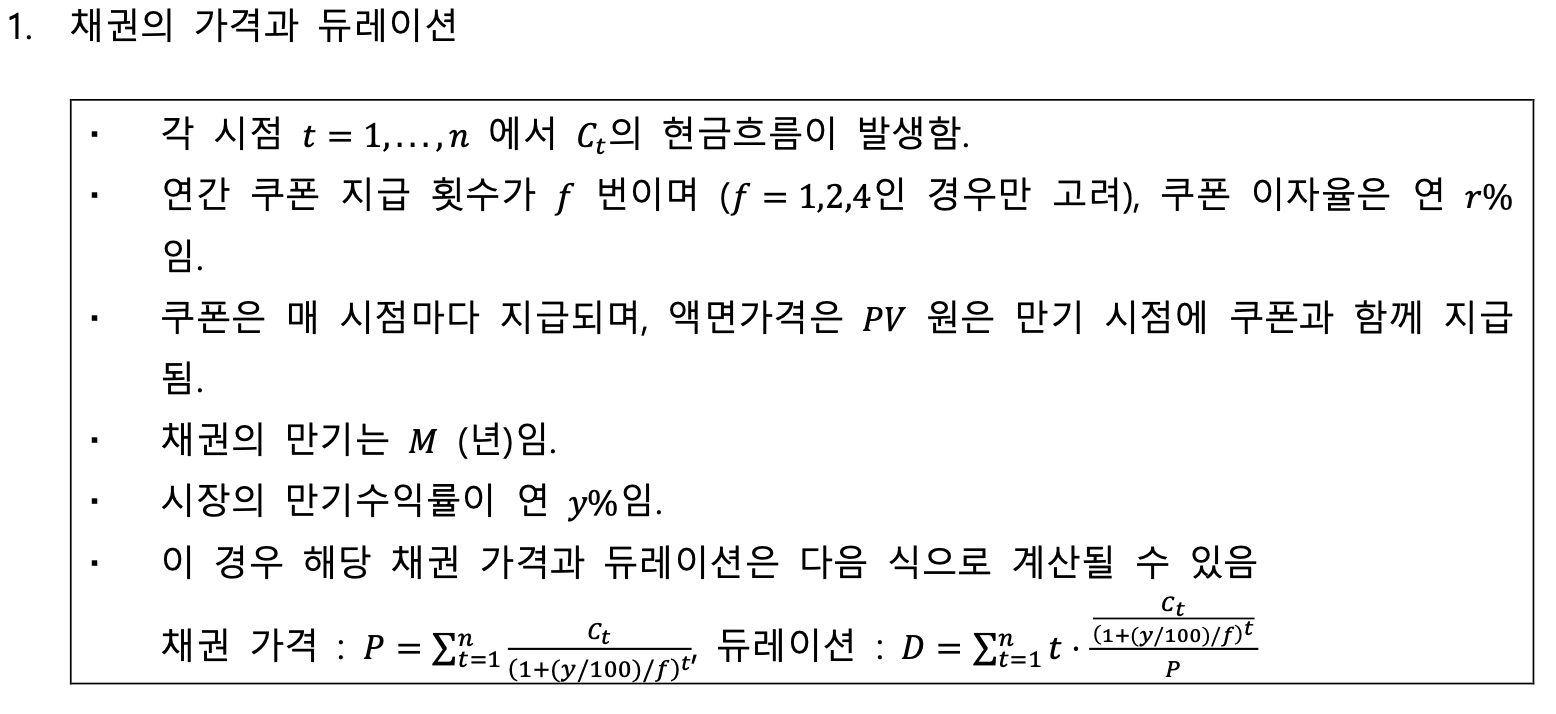
\includegraphics{images/Python_midterm1.png}

\subsection*{(1)}\label{section-10}
\addcontentsline{toc}{subsection}{(1)}

5개의 인자 facevalue=𝑃𝑉, couprate=𝑟, yield=𝑦, maturity=𝑀으로 입력하고,
frequency=𝑓에 맞게 ``annual'', ``semi-annual'', ``quarterly'' 중 하나의
문자 값으로 입력하면, 위 식에 따라 계산된 채권가격과 듀레이션을 아래와
같은 형태의 튜플로 반환하는 함수 bondftn을 작성하여라.

\begin{Shaded}
\begin{Highlighting}[]
\KeywordTok{def}\NormalTok{ bondftn(pv,r,y,m,f}\OperatorTok{=}\StringTok{"annual"}\NormalTok{,rnd}\OperatorTok{=}\DecValTok{3}\NormalTok{):}
    \ControlFlowTok{if} \BuiltInTok{type}\NormalTok{(pv)}\OperatorTok{!=}\BuiltInTok{float} \KeywordTok{and} \BuiltInTok{type}\NormalTok{(pv)}\OperatorTok{!=}\BuiltInTok{int}\NormalTok{ : }\ControlFlowTok{return} \BuiltInTok{print}\NormalTok{(}\StringTok{"error: pv should be number!!!"}\NormalTok{)}
    \ControlFlowTok{if} \BuiltInTok{type}\NormalTok{(r)}\OperatorTok{!=}\BuiltInTok{float} \KeywordTok{and} \BuiltInTok{type}\NormalTok{(r)}\OperatorTok{!=}\BuiltInTok{int}\NormalTok{: }\ControlFlowTok{return} \BuiltInTok{print}\NormalTok{(}\StringTok{"error: r should be number!!!"}\NormalTok{)}
    \ControlFlowTok{if} \BuiltInTok{type}\NormalTok{(y)}\OperatorTok{!=}\BuiltInTok{float} \KeywordTok{and} \BuiltInTok{type}\NormalTok{(y)}\OperatorTok{!=}\BuiltInTok{int}\NormalTok{: }\ControlFlowTok{return} \BuiltInTok{print}\NormalTok{(}\StringTok{"error: y should be number!!!"}\NormalTok{)}
    \ControlFlowTok{if} \BuiltInTok{type}\NormalTok{(m)}\OperatorTok{!=}\BuiltInTok{int}\NormalTok{: }\ControlFlowTok{return} \BuiltInTok{print}\NormalTok{(}\StringTok{"error: M should be integer!!!"}\NormalTok{)}
    \ControlFlowTok{if}\NormalTok{ f}\OperatorTok{==}\StringTok{"annual"}\NormalTok{: fre}\OperatorTok{=}\DecValTok{1}
    \ControlFlowTok{elif}\NormalTok{ f}\OperatorTok{==}\StringTok{"semi{-}annual"}\NormalTok{: fre}\OperatorTok{=}\DecValTok{2}
    \ControlFlowTok{elif}\NormalTok{ f}\OperatorTok{==}\StringTok{"quarterly"}\NormalTok{: fre}\OperatorTok{=}\DecValTok{4}
    \ControlFlowTok{else}\NormalTok{: }\ControlFlowTok{return} \BuiltInTok{print}\NormalTok{(}\StringTok{"error: f can be \textquotesingle{}annual\textquotesingle{}, \textquotesingle{}semi{-}annual\textquotesingle{}, \textquotesingle{}quarterly\textquotesingle{}"}\NormalTok{)}
\NormalTok{    n}\OperatorTok{=}\NormalTok{fre}\OperatorTok{*}\NormalTok{m}
\NormalTok{    coupon}\OperatorTok{=}\NormalTok{pv}\OperatorTok{*}\NormalTok{r}\OperatorTok{/}\DecValTok{100}\OperatorTok{/}\NormalTok{fre}
\NormalTok{    price}\OperatorTok{=}\FloatTok{0.0}
\NormalTok{    value\_duration}\OperatorTok{=}\FloatTok{0.0}
    \ControlFlowTok{for}\NormalTok{ i }\KeywordTok{in} \BuiltInTok{range}\NormalTok{(n):}
        \ControlFlowTok{if}\NormalTok{ i}\OperatorTok{==}\NormalTok{n}\OperatorTok{{-}}\DecValTok{1}\NormalTok{: cf\_i}\OperatorTok{=}\NormalTok{pv}\OperatorTok{+}\NormalTok{coupon}
        \ControlFlowTok{else}\NormalTok{: cf\_i}\OperatorTok{=}\NormalTok{coupon}
\NormalTok{        pv\_cf\_i}\OperatorTok{=}\NormalTok{cf\_i}\OperatorTok{/}\NormalTok{((}\DecValTok{1}\OperatorTok{+}\NormalTok{(y}\OperatorTok{/}\DecValTok{100}\OperatorTok{/}\NormalTok{fre))}\OperatorTok{**}\NormalTok{(i}\OperatorTok{+}\DecValTok{1}\NormalTok{))}
\NormalTok{        tw\_pv\_cf\_i}\OperatorTok{=}\NormalTok{((i}\OperatorTok{+}\DecValTok{1}\NormalTok{)}\OperatorTok{/}\NormalTok{fre)}\OperatorTok{*}\NormalTok{cf\_i}\OperatorTok{/}\NormalTok{(}\DecValTok{1}\OperatorTok{+}\NormalTok{(y}\OperatorTok{/}\DecValTok{100}\OperatorTok{/}\NormalTok{fre))}\OperatorTok{**}\NormalTok{(i}\OperatorTok{+}\DecValTok{1}\NormalTok{)}
\NormalTok{        price}\OperatorTok{+=}\NormalTok{pv\_cf\_i}
\NormalTok{        value\_duration}\OperatorTok{+=}\NormalTok{tw\_pv\_cf\_i}
\NormalTok{    duration}\OperatorTok{=}\NormalTok{value\_duration}\OperatorTok{/}\NormalTok{price}
\NormalTok{    result}\OperatorTok{=}\NormalTok{(}\BuiltInTok{round}\NormalTok{(price,rnd),}\BuiltInTok{round}\NormalTok{(duration,rnd))}
    \ControlFlowTok{return}\NormalTok{ result}
\end{Highlighting}
\end{Shaded}

\begin{Shaded}
\begin{Highlighting}[]
\NormalTok{bondftn(pv}\OperatorTok{=}\DecValTok{100}\NormalTok{,r}\OperatorTok{=}\DecValTok{5}\NormalTok{,y}\OperatorTok{=}\FloatTok{4.5}\NormalTok{,m}\OperatorTok{=}\DecValTok{2}\NormalTok{,f}\OperatorTok{=}\StringTok{"quarterly"}\NormalTok{)}
\end{Highlighting}
\end{Shaded}

\begin{verbatim}
(100.951, 1.916)
\end{verbatim}

\subsection*{(2)}\label{section-11}
\addcontentsline{toc}{subsection}{(2)}

만기 M이 5, 4, 3, 2, 1인 각 경우에 대해, 쿠폰이자율이 5\%, 4\%, 3\%,
2\%, 1\% 인 각각에 대하여 만기수익률이 10\%에 11\%로 상승함에 따라 채권
가격의 변화율이 몇 \%인지를 모두 계산한 뒤, 아래와 같은 중첩된 딕셔너리
result\_dict으로 저장하여라.

단, 액면가는 100, 쿠폰 지급 횟수는 연간 1회라고 하자.

\begin{Shaded}
\begin{Highlighting}[]
\NormalTok{result\_dict}\OperatorTok{=}\BuiltInTok{dict}\NormalTok{()}
\ControlFlowTok{for}\NormalTok{ i }\KeywordTok{in} \BuiltInTok{range}\NormalTok{(}\DecValTok{5}\NormalTok{):}
\NormalTok{    m\_i}\OperatorTok{=}\DecValTok{5}\OperatorTok{{-}}\NormalTok{i}
\NormalTok{    result\_dict[}\StringTok{\textquotesingle{}M=\textquotesingle{}}\OperatorTok{+}\BuiltInTok{str}\NormalTok{(m\_i)]}\OperatorTok{=}\BuiltInTok{dict}\NormalTok{()}
    \ControlFlowTok{for}\NormalTok{ j }\KeywordTok{in} \BuiltInTok{range}\NormalTok{(}\DecValTok{5}\NormalTok{):}
\NormalTok{        r\_j}\OperatorTok{=}\DecValTok{5}\OperatorTok{{-}}\NormalTok{j}
\NormalTok{        price\_before}\OperatorTok{=}\NormalTok{bondftn(pv}\OperatorTok{=}\DecValTok{100}\NormalTok{,r}\OperatorTok{=}\NormalTok{r\_j,y}\OperatorTok{=}\DecValTok{10}\NormalTok{,m}\OperatorTok{=}\NormalTok{m\_i,f}\OperatorTok{=}\StringTok{"annual"}\NormalTok{)[}\DecValTok{0}\NormalTok{]}
\NormalTok{        price\_after}\OperatorTok{=}\NormalTok{bondftn(pv}\OperatorTok{=}\DecValTok{100}\NormalTok{,r}\OperatorTok{=}\NormalTok{r\_j,y}\OperatorTok{=}\DecValTok{11}\NormalTok{,m}\OperatorTok{=}\NormalTok{m\_i,f}\OperatorTok{=}\StringTok{"annual"}\NormalTok{)[}\DecValTok{0}\NormalTok{]}
\NormalTok{        price\_return}\OperatorTok{=}\NormalTok{(price\_after}\OperatorTok{{-}}\NormalTok{price\_before)}\OperatorTok{/}\NormalTok{price\_before}
\NormalTok{        result\_dict[}\StringTok{\textquotesingle{}M=\textquotesingle{}}\OperatorTok{+}\BuiltInTok{str}\NormalTok{(m\_i)][}\BuiltInTok{str}\NormalTok{(r\_j)}\OperatorTok{+}\StringTok{\textquotesingle{}\%\textquotesingle{}}\NormalTok{]}\OperatorTok{=}\BuiltInTok{round}\NormalTok{(price\_return,}\DecValTok{5}\NormalTok{)}
\NormalTok{result\_dict}
\end{Highlighting}
\end{Shaded}

\begin{verbatim}
{'M=5': {'5%': -0.03974,
  '4%': -0.04046,
  '3%': -0.04126,
  '2%': -0.04215,
  '1%': -0.04314},
 'M=4': {'5%': -0.03287,
  '4%': -0.03332,
  '3%': -0.03381,
  '2%': -0.03434,
  '1%': -0.03491},
 'M=3': {'5%': -0.02544,
  '4%': -0.02568,
  '3%': -0.02593,
  '2%': -0.02619,
  '1%': -0.02648},
 'M=2': {'5%': -0.01749,
  '4%': -0.01758,
  '3%': -0.01765,
  '2%': -0.01776,
  '1%': -0.01784},
 'M=1': {'5%': -0.00901,
  '4%': -0.009,
  '3%': -0.009,
  '2%': -0.009,
  '1%': -0.00901}}
\end{verbatim}

\begin{Shaded}
\begin{Highlighting}[]
\NormalTok{result\_dict[}\StringTok{\textquotesingle{}M=5\textquotesingle{}}\NormalTok{][}\StringTok{\textquotesingle{}5\%\textquotesingle{}}\NormalTok{]}
\end{Highlighting}
\end{Shaded}

\begin{verbatim}
-0.03974
\end{verbatim}

\subsection*{(3)}\label{section-12}
\addcontentsline{toc}{subsection}{(3)}

만기 M이 5, 4, 3, 2, 1인 각 경우에 대해, 쿠폰이자율이 5\%, 4\%, 3\%,
2\%, 1\% 인 각각에 대하여 만기수익률이 10\%로 주어졌을 때의 듀레이션을
(1)에서의 bondftn을 활용하여 모두 계산하여라.

또한 이를 (2)에서와 동일한 구조를 가지는 (중첩된) 딕셔너리
result\_dict\_dur에 저장하여라.

즉 아래와 같은 방식으로 값을 추출할 수 있어야 한다. 단, 여기서도
액면가는 100, 쿠폰 지급 횟수는 연간 1회라고 하자.

\begin{Shaded}
\begin{Highlighting}[]
\NormalTok{result\_dict\_dur}\OperatorTok{=}\BuiltInTok{dict}\NormalTok{()}
\ControlFlowTok{for}\NormalTok{ i }\KeywordTok{in} \BuiltInTok{range}\NormalTok{(}\DecValTok{5}\NormalTok{):}
\NormalTok{    m\_i}\OperatorTok{=}\DecValTok{5}\OperatorTok{{-}}\NormalTok{i}
\NormalTok{    result\_dict\_dur[}\StringTok{\textquotesingle{}M=\textquotesingle{}}\OperatorTok{+}\BuiltInTok{str}\NormalTok{(m\_i)]}\OperatorTok{=}\BuiltInTok{dict}\NormalTok{()}
    \ControlFlowTok{for}\NormalTok{ j }\KeywordTok{in} \BuiltInTok{range}\NormalTok{(}\DecValTok{5}\NormalTok{):}
\NormalTok{        r\_j}\OperatorTok{=}\DecValTok{5}\OperatorTok{{-}}\NormalTok{j}
\NormalTok{        result\_dict\_dur[}\StringTok{\textquotesingle{}M=\textquotesingle{}}\OperatorTok{+}\BuiltInTok{str}\NormalTok{(m\_i)][}\BuiltInTok{str}\NormalTok{(r\_j)}\OperatorTok{+}\StringTok{\textquotesingle{}\%\textquotesingle{}}\NormalTok{]}\OperatorTok{=}\NormalTok{bondftn(pv}\OperatorTok{=}\DecValTok{100}\NormalTok{,r}\OperatorTok{=}\NormalTok{r\_j,}
\NormalTok{                                                             y}\OperatorTok{=}\DecValTok{10}\NormalTok{,m}\OperatorTok{=}\NormalTok{m\_i,}
\NormalTok{                                                             f}\OperatorTok{=}\StringTok{"annual"}\NormalTok{,rnd}\OperatorTok{=}\DecValTok{5}\NormalTok{)[}\DecValTok{1}\NormalTok{]}
\NormalTok{result\_dict\_dur}
\end{Highlighting}
\end{Shaded}

\begin{verbatim}
{'M=5': {'5%': 4.48786,
  '4%': 4.57019,
  '3%': 4.66101,
  '2%': 4.76171,
  '1%': 4.874},
 'M=4': {'5%': 3.6951,
  '4%': 3.74653,
  '3%': 3.80216,
  '2%': 3.8625,
  '1%': 3.9282},
 'M=3': {'5%': 2.84899,
  '4%': 2.87566,
  '3%': 2.90394,
  '2%': 2.93397,
  '1%': 2.96593},
 'M=2': {'5%': 1.95023,
  '4%': 1.95941,
  '3%': 1.96896,
  '2%': 1.97889,
  '1%': 1.98923},
 'M=1': {'5%': 1.0, '4%': 1.0, '3%': 1.0, '2%': 1.0, '1%': 1.0}}
\end{verbatim}

\begin{Shaded}
\begin{Highlighting}[]
\NormalTok{result\_dict\_dur[}\StringTok{\textquotesingle{}M=5\textquotesingle{}}\NormalTok{][}\StringTok{\textquotesingle{}4\%\textquotesingle{}}\NormalTok{]}
\end{Highlighting}
\end{Shaded}

\begin{verbatim}
4.57019
\end{verbatim}

\section*{Problem 2.}\label{problem-2.}
\addcontentsline{toc}{section}{Problem 2.}

\markright{Problem 2.}

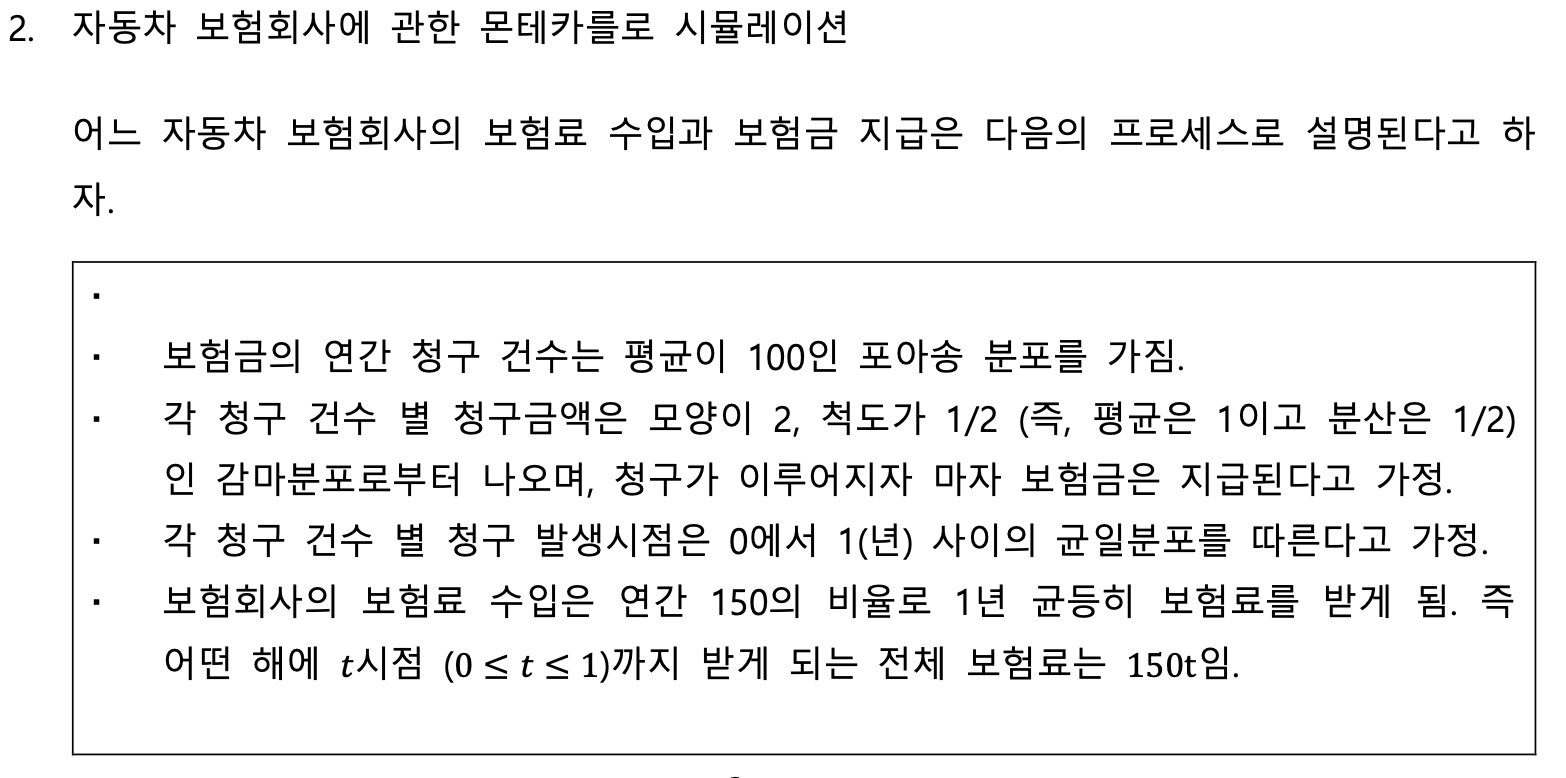
\includegraphics{images/Python_midterm2.png}

\subsection*{(1)}\label{section-13}
\addcontentsline{toc}{subsection}{(1)}

어떤 1년 동안 발생하는 모든 청구들의 시간과 금액을 모의실험해 보자.

0에서 시작하여1년 동안 보험회사의 잔고를 계산한 뒤 balance라는 리스트로
저장하여라.

단, balance의 첫번째 값은 0이며, 보험 청구가 발생하는 시점(𝑡)에만, 해당
시점의 balance (그 시점까지 받은 보험료 수익(150𝑡)을 더하고, 그 시점에서
청구로 지급되는 보험금을 빼 주는 방식)를 계산하여 순서대로 저장할 것.

\textbf{Answer}

먼저, 보험금의 연간 청구건수가 평균이 100인 포아송분포를 따르므로
\(pmf,\;P(X=x)=\frac{\lambda^xe^{-\lambda}}{x!},\;\lambda=100\)입니다.

다음으로, 보험금의 청구금액은 평균은 1, 분산은 1/2인 감마분포를 따르므로
\(pdf,\;f(x)=x^{k-1}\frac{e^{-x/\theta}}{\theta^k\Gamma(k)},\;k\theta=1,\;k\theta^2=1/2\)입니다.
즉, \(k=2,\;\theta=1/2\)입니다.

각 청구금액은 즉시 지급되며, 발생시점은 0\textasciitilde1 사이의 uniform
distribution을 따르므로 \(pdx.\;f(x)=\frac{1}{1-0}=1\)입니다.

이제, 1년간 발생하는 보험손익의 모의실험에 대한 청구건수(포아송분포)를
\(N\)번이라고 하고, 청구금액(감마분포) 및 청구시점(균등분포)를 각각
\(g_i\)와 \(t_i\; for\; 1,...,N\)라고 하면, \(t=t_i\) 시점의 balance는
아래와 같이 계산됩니다.

\[{balance}_{t_i}=150t_i-\sum_{k=1}^{i}g_k\]

또한, 기말시점(t=1)의 최종 balance는 \(150-\sum_{all\;k}g_k\)가 됩니다.

\begin{Shaded}
\begin{Highlighting}[]
\CommentTok{\# 포아송, 감마, 균등분포에 다한 모의실험은 numpy의 random module 활용}
\ImportTok{import}\NormalTok{ numpy }\ImportTok{as}\NormalTok{ np}
\ImportTok{from}\NormalTok{ numpy }\ImportTok{import}\NormalTok{ random }\ImportTok{as}\NormalTok{ rd}


\NormalTok{rd.seed(}\DecValTok{0}\NormalTok{) }\CommentTok{\# seed를 설정하여 통제}
\NormalTok{N}\OperatorTok{=}\NormalTok{rd.poisson(lam}\OperatorTok{=}\DecValTok{100}\NormalTok{,size}\OperatorTok{=}\DecValTok{1}\NormalTok{)}
\NormalTok{N}\OperatorTok{=}\NormalTok{N[}\DecValTok{0}\NormalTok{]}
\NormalTok{t}\OperatorTok{=}\NormalTok{rd.uniform(low}\OperatorTok{=}\FloatTok{0.0}\NormalTok{,high}\OperatorTok{=}\FloatTok{1.0}\NormalTok{,size}\OperatorTok{=}\NormalTok{N)}
\NormalTok{t}\OperatorTok{=}\NormalTok{np.sort(t)}
\NormalTok{g}\OperatorTok{=}\NormalTok{rd.gamma(shape}\OperatorTok{=}\FloatTok{2.}\NormalTok{,scale}\OperatorTok{=}\FloatTok{0.5}\NormalTok{,size}\OperatorTok{=}\NormalTok{N)}
\NormalTok{balance}\OperatorTok{=}\NormalTok{[}\DecValTok{0}\NormalTok{] }\CommentTok{\# balance의 초기값은 0}
\ControlFlowTok{for}\NormalTok{ i }\KeywordTok{in} \BuiltInTok{range}\NormalTok{(N):}
\NormalTok{    balance.append(}\BuiltInTok{round}\NormalTok{(t[i]}\OperatorTok{*}\DecValTok{150}\OperatorTok{{-}}\BuiltInTok{sum}\NormalTok{(g[:i}\OperatorTok{+}\DecValTok{1}\NormalTok{]),}\DecValTok{4}\NormalTok{))}
\NormalTok{balance.append(}\BuiltInTok{round}\NormalTok{(}\DecValTok{150}\OperatorTok{{-}}\BuiltInTok{sum}\NormalTok{(g),}\DecValTok{4}\NormalTok{)) }\CommentTok{\# balance의 기말값}
\end{Highlighting}
\end{Shaded}

\begin{Shaded}
\begin{Highlighting}[]
\BuiltInTok{print}\NormalTok{(balance[:}\DecValTok{5}\NormalTok{],balance[N}\OperatorTok{{-}}\DecValTok{5}\NormalTok{:],sep}\OperatorTok{=}\StringTok{"}\CharTok{\textbackslash{}n}\StringTok{"}\NormalTok{)}
\end{Highlighting}
\end{Shaded}

\begin{verbatim}
[0, -1.9755, -2.1182, -2.7092, -3.9799]
[44.5214, 47.2399, 48.4395, 48.2655, 47.6871, 48.74, 50.4839]
\end{verbatim}

\subsection*{(2)}\label{section-14}
\addcontentsline{toc}{subsection}{(2)}

위 모의실험을 10000회 반복하여 다음에 대한 확률을 추정해 보자.

\begin{itemize}
\item
  보험회사가 최종적으로 가지게 되는 balance의 기대값(모의실험을 10000회
  반복하였을 때 각 모의실험마다 계산된 balance의 최종값들의 평균으로
  추정)은 얼마인가?
\item
  보험회사의 balance가 1년 중 한번 이상 -5 이하로 떨어질 확률(10000회의
  모의실험 중에서 balance가 -5이하로 떨어진 적이 있었던 경우의 비율로
  추정)은 얼마인가?
\end{itemize}

\textbf{Answer}

평균은 약 49.86, -5이하로 떨어질 확률은 약 7.05\%입니다.

\begin{Shaded}
\begin{Highlighting}[]
\NormalTok{last\_balance}\OperatorTok{=}\BuiltInTok{list}\NormalTok{()}
\NormalTok{minus5\_balance}\OperatorTok{=}\DecValTok{0}
\ControlFlowTok{for}\NormalTok{ k }\KeywordTok{in} \BuiltInTok{range}\NormalTok{(}\DecValTok{10000}\NormalTok{):}
\NormalTok{    rd.seed(k)}
\NormalTok{    N}\OperatorTok{=}\NormalTok{rd.poisson(lam}\OperatorTok{=}\DecValTok{100}\NormalTok{,size}\OperatorTok{=}\DecValTok{1}\NormalTok{)}
\NormalTok{    N}\OperatorTok{=}\NormalTok{N[}\DecValTok{0}\NormalTok{]}
\NormalTok{    t}\OperatorTok{=}\NormalTok{rd.uniform(low}\OperatorTok{=}\FloatTok{0.0}\NormalTok{,high}\OperatorTok{=}\FloatTok{1.0}\NormalTok{,size}\OperatorTok{=}\NormalTok{N)}
\NormalTok{    t}\OperatorTok{=}\NormalTok{np.sort(t)}
\NormalTok{    g}\OperatorTok{=}\NormalTok{rd.gamma(shape}\OperatorTok{=}\FloatTok{2.}\NormalTok{,scale}\OperatorTok{=}\FloatTok{0.5}\NormalTok{,size}\OperatorTok{=}\NormalTok{N)}
\NormalTok{    balance}\OperatorTok{=}\NormalTok{[}\DecValTok{0}\NormalTok{]}
    \ControlFlowTok{for}\NormalTok{ i }\KeywordTok{in} \BuiltInTok{range}\NormalTok{(N):}
\NormalTok{        balance.append(}\BuiltInTok{round}\NormalTok{(t[i]}\OperatorTok{*}\DecValTok{150}\OperatorTok{{-}}\BuiltInTok{sum}\NormalTok{(g[:i}\OperatorTok{+}\DecValTok{1}\NormalTok{]),}\DecValTok{4}\NormalTok{))}
\NormalTok{    last\_balance.append(}\BuiltInTok{round}\NormalTok{(}\DecValTok{150}\OperatorTok{{-}}\BuiltInTok{sum}\NormalTok{(g),}\DecValTok{4}\NormalTok{))}
\NormalTok{    balance.sort()}
    \ControlFlowTok{if}\NormalTok{ balance[}\DecValTok{0}\NormalTok{]}\OperatorTok{\textless{}={-}}\DecValTok{5}\NormalTok{:minus5\_balance}\OperatorTok{+=}\DecValTok{1}
\BuiltInTok{print}\NormalTok{(}\BuiltInTok{sum}\NormalTok{(last\_balance)}\OperatorTok{/}\DecValTok{10000}\NormalTok{,}
\NormalTok{      minus5\_balance}\OperatorTok{/}\DecValTok{10000}\NormalTok{,sep}\OperatorTok{=}\StringTok{"}\CharTok{\textbackslash{}n}\StringTok{"}\NormalTok{)}
\end{Highlighting}
\end{Shaded}

\begin{verbatim}
49.864134890000095
0.0705
\end{verbatim}

\part{채권분석\&기간구조('24봄)}

\chapter*{채권분석 과제1}\label{uxcc44uxad8cuxbd84uxc11d-uxacfcuxc81c1}
\addcontentsline{toc}{chapter}{채권분석 과제1}

\markboth{채권분석 과제1}{채권분석 과제1}

\section*{1. CB}\label{cb}
\addcontentsline{toc}{section}{1. CB}

\markright{1. CB}

\textbf{\emph{(Question)}}

전환사채를 액면 F 만큼 매입할 때 전환가가 P라면, 전환주식수는 F/P 로
주어진다. 특정 전환사채를 액면 1억원 만큼 시장에서 매입하였다. 매입가는
1억 1천만원이다. 전환가격은 5만원으로 주어져 있다.

해당 주식의 시장가 가 6만원일 때 전환하여 매도하였다면 투자자의
수익률은무엇인가? \% 로 쓰되, 소수점 둘째 자리까지만 쓰시오.

\textbf{\emph{(Answer)}} 9.09\%

\[전환주식수 = \frac{1억원}{5만원} = 2,000주\]
\[전환주식의 가치 = 2000\times 60,000원=1억\,2천만원\]
\[투자원금=1억1천만원, 수익률=\frac{1.2억}{1.1억}-1\approx 9.09\%\]

\section*{2. FRN}\label{frn}
\addcontentsline{toc}{section}{2. FRN}

\markright{2. FRN}

\textbf{\emph{(Question)}}

정부가 2년 만기 변동금리채권을 발행한다고 가정하자. 기준금리는 만기 1년
현물 이자율 (spot rate 또는 1년 만기 무이표채 국채의 이자율) 이고, 해당
변동금리채권의 이자는 1년마다 계산하여 지급한다, 즉 1년 말에 지급하고
2년 만기시 원금과 함께 지급한다.

현재 1년 spot rate 을 \(r_{1,0}\), 1년 후 spot rate 을 \(r_{1,1}\) 이라
하면 받게 되는 총 금액은 액면 100 당 \(100r_{1,0}\) (1년 시점) 과
\(100(1 + r_{1,1})\) (2년 시점)이다. 물론 \(r_{1,1}\) 은 현재 시점에서는
알 수 없는 확률변수이다.

액면이 100 인 위의 2년 만기 변동금리채권의 현재 시점의 공정한 가격을
구하시오. 투자자는 시장에서 1년 만기 무이표채 국채를 현재 시점이던 1년
후 시점이던 자유롭게 거래할 수 있다.

\textbf{\emph{(Answer)}} 100

상기 FRN은 1년 만기 무이표 국채의 이자율만큼의 쿠폰을 지급하고 있다.
이러한 액면 100인 FRN의 현금흐름은 현재 1년 만기 무이표국채에
\(100r_{1,0}\)만큼 투자하고, 1년 뒤 만기시점에 다시 1년 만기
무이표국채에 \(100+r_{1,1}\)투자함으로써 복제할 수 있다.

즉, 해당 FRN은 무위험이자율 만큼의 연수익률을 보장하는 채권으로서
쿠폰=할인율이므로 \textbf{공정가격은 100(par-value)}에 형성되어야 한다.

\begin{tcolorbox}[enhanced jigsaw, toprule=.15mm, colframe=quarto-callout-note-color-frame, opacitybacktitle=0.6, bottomtitle=1mm, left=2mm, breakable, coltitle=black, title=\textcolor{quarto-callout-note-color}{\faInfo}\hspace{0.5em}{Foward rate를 이용한 풀이}, colbacktitle=quarto-callout-note-color!10!white, opacityback=0, bottomrule=.15mm, toptitle=1mm, leftrule=.75mm, titlerule=0mm, colback=white, arc=.35mm, rightrule=.15mm]

\(r_{1,1}\)은 확률변수이므로, FRN의 2년뒤 현금흐름 \(100(1+r_{1,1})\)을
현재가치로 환산한다면 그 공정가치는
\(\frac{100(1+E[r_{1,1}])}{(1+r_{2,0})^2}\)으로 표현할 수 있다.

한편, 1년뒤 1년 spot-rate의 기댓값은 foward rate으로 볼 수 있고,
현재시점의 2년 spot-rate는 \((1+r_{1,0})(1+f_{1,1})\)로 표현할 수 있다.
따라서, FRN의 공정가격은 다음과 같다.

\[FRN\; price=\frac{100r_{1.0}}{1+r_{1,0}}+\frac{100(1+E[r_{1,1}])}{1+r_{2,0}}=\frac{100r_{1.0}}{1+r_{1,0}}+\frac{100(1+f_{1,1})}{(1+r_{1,0})(1+f_{1,1})}=\frac{100(1+r_{1,0})}{1+r_{1,0}}=100\]

\end{tcolorbox}

\section*{3. YTM}\label{ytm}
\addcontentsline{toc}{section}{3. YTM}

\markright{3. YTM}

\textbf{\emph{(Question)}}

잔존만기가 3년이고 연 8\% 이자를 6개월마다 제공하는 채권을 가정하자. A
투자자는 이 채권에 관심이 있고 거래하는 딜러는 100달러 액면당 92.5067
달러를 요구한다.

이때 이 채권의 수익률은 얼마인가? \% 로 표시하되 소수점은 반올림하여
정수로 나타내시오.

\textbf{\emph{(Answer)}} 11\%

채권의 수익률 \(y\)와 가격에 관한 산식은 다음과 같다.

\[92.5067=\sum_{k=1}^6\frac{8/2}{(1+y/2)^{k}}+\frac{100}{(1+y/2)^{6}}\]

이를 엑셀 해찾기 기능으로 근사한 \(y\)값은 약 11\%이다.

\section*{4. Continuous compounding}\label{continuous-compounding}
\addcontentsline{toc}{section}{4. Continuous compounding}

\markright{4. Continuous compounding}

\textbf{\emph{(Question)}} 10.71\%

위의 문제는 compounding frequency 를 연 1회로 가정하고 있다. 이것은
이산복리법이다. 이 frequency가 무한이 되는 연속복리법에 따르면 1달러
투자가 1년 후에 \(e^y\) 가 된다. 여기서 \(y\) 는 연속복리이자율이다.

위 현금흐름 수익률을 연속복리이자율로 표현하시오. \%로 나타내되 소수점
둘째 자리까지 쓰시오.

\textbf{\emph{(Answer)}}

(3)의 현금흐름을 연속복리로 표현하면 다음과 같다.

\[92.5067=\sum_{k=1}^6\frac{8}{2}e^{-0.5ky}+100e^{-3y}\]

이를 엑셀 해찾기 기능으로 근사한 \(y\)값은 10.71\%이다.

\begin{tcolorbox}[enhanced jigsaw, toprule=.15mm, colframe=quarto-callout-note-color-frame, opacitybacktitle=0.6, bottomtitle=1mm, left=2mm, breakable, coltitle=black, title=\textcolor{quarto-callout-note-color}{\faInfo}\hspace{0.5em}{수익률 관계를 이용한 풀이}, colbacktitle=quarto-callout-note-color!10!white, opacityback=0, bottomrule=.15mm, toptitle=1mm, leftrule=.75mm, titlerule=0mm, colback=white, arc=.35mm, rightrule=.15mm]

(3)의 수식과 비교하여 단순히
\(e^{0.5y_{continuous}}=(1+y_{annual}/2)=1.055\)로 표현할 수 있고 값은
10.71\%로 오차범위 내에서 동일하다.

\end{tcolorbox}

\section*{5. Arbitrage}\label{arbitrage}
\addcontentsline{toc}{section}{5. Arbitrage}

\markright{5. Arbitrage}

\textbf{\emph{(Question)}}

아래와 같은 세 개의 채권이 시장에서 거래되고 있다. 트레이더 B 는 이를
보고 곧 차익거래의 기회가 있음을 파악하고 전략적으로 거래하여 이익을
얻었다. 어떤 전략이 가능할지 본인의 생각을 기술하시오.

\begin{itemize}
\tightlist
\item
  채권 a: 만기 1년 무이표채, 액면 100 당 가격 90
\item
  채권 b: 만기 2년 무이표채, 액면 100 당 가격 80
\item
  채권 c: 만기 2년 이표채, coupon rate 10\%, 매년 말 이자지급, 액면 100
  당 가격 100
\end{itemize}

\textbf{\emph{(Answer)}} 채권a:채권b=1:11로 투자하여 채권c를 만들고
시장에 매도

채권a와 채권b의 수익률은 zero-rates이며, 이를 \(y_a,y_b\)라고 할 때,
다음과 같이 쓸 수 있다.
\[\frac{100}{1+y_a}=90,\; \frac{100}{(1+y_b)^2}=80 \Rightarrow \frac{1}{1+y_a}=0.9,\;\frac{1}{(1+y_b)^2}=0.8\]

이를 이용하여 채권c의 현금흐름을 평가하면,
\(\frac{10}{1+y_a}+\frac{110}{(1+y_b)^2}=9+88=97\)

즉, \textbf{액면 100인 채권c의 공정가격은 97이나, 현재 100에 거래되고
있으므로 3만큼 고평가}되어있는 상태이다. 따라서 트레이더B가
\textbf{채권a:채권b=1:11 비중으로 매수한다면 액면이 10인 채권c의
현금흐름을 정확하게 복제}할 수 있는데, 이를 이용하면 무위험 차익거래를
할 수 있다.

예를 들어,

\begin{enumerate}
\def\labelenumi{(\arabic{enumi})}
\item
  액면 100억원 채권c를 시장에 매도(공매도 or 발행)하여 100억원의 자금을
  조달
\item
  액면 10억원 채권a를 9억원에, 액면 110억원 채권b를 88억원에 매수
\item
  1년뒤 채권a의 원금 10억을 받아 채권c의 이표 10억원을 값고, 2년뒤
  채권b의 원금 110억을 받아 채권c의 원금+이표 110억원을 값을 수 있으므로
  현재 시점에서 미래현금흐름은 0임(리스크=0)
\item
  한편, 현재 100억원을 빌려 97억원을 사용하였으므로 3억원의 무위험차익
  실현 (또는, 남은 3억원을 채권b에 투자하여 현재시점의 투입자본없이
  2년뒤 3.75억의 수익 실현 가능)
\end{enumerate}

\chapter*{채권분석 과제2}\label{uxcc44uxad8cuxbd84uxc11d-uxacfcuxc81c2}
\addcontentsline{toc}{chapter}{채권분석 과제2}

\markboth{채권분석 과제2}{채권분석 과제2}

\section*{1. Callable bond}\label{callable-bond}
\addcontentsline{toc}{section}{1. Callable bond}

\markright{1. Callable bond}

\textbf{\emph{(Question)}}

만기 2년, 액면이자율 10\% (연 1회 지급), 액면가 100 인 수의상환채권
callable bond 를 생각하자. 이 채권의 상환액 call price 는 100,
상환기간은 1년부터 (이자지급 이후) 만기까지 이다. 즉, 채권발행자
(기채자, 채무자) 는 상환기간 동안 원하는 때 100으로 채권을 상환할 수
있다. 1년이 지난 시점에서 만기수익률을 10.05\% 라 가정하자.

채권의 가격 \(P_0\) 를 구하시오.

시중금리변화에 따라 이 만기수익률이 즉각적으로 10bp 상승할 때의 가격
\(P_+\) 를 구하시오.

그리고 만기수익률이 즉각적으로 10bp 하락할 때의 가격 \(P_−\) 를
구하시오.

채권발행자는 채권의 가치가 100을 넘어서면 상환할 인센티브가 있음을
고려하라. 이들 세 값을 바탕으로 우리는 수의상환채권에 대하여 유효한
듀레이션을 \(-\frac{1}{P_0}\times\frac{P_+-P_-}{20bp}\)로 구할 수 있다.
소수점 네째자리까지 리포트하시오.

\textbf{\emph{(Answer)}}

1년이 지난 시점에서 수의상환채권의 잔여현금흐름은 만기 일시납 110이며,
YTM은 10.05\%이므로 가격 \(P_0\)는 약 99.9546입니다.

\begin{Shaded}
\begin{Highlighting}[]
\NormalTok{P0}\OtherTok{=}\DecValTok{110}\SpecialCharTok{/}\NormalTok{(}\DecValTok{1}\FloatTok{+0.1005}\NormalTok{)}
\NormalTok{P0}
\end{Highlighting}
\end{Shaded}

\begin{verbatim}
[1] 99.95457
\end{verbatim}

만기수익률이 10bp씩 즉각적으로 움직일 때, 수의상환부를 고려하지 않은
채권가격은 아래와 같습니다.

\begin{Shaded}
\begin{Highlighting}[]
\NormalTok{P0\_up}\OtherTok{=}\DecValTok{110}\SpecialCharTok{/}\NormalTok{(}\DecValTok{1}\FloatTok{+0.1005+0.001}\NormalTok{)}
\NormalTok{P0\_down}\OtherTok{=}\DecValTok{110}\SpecialCharTok{/}\NormalTok{(}\DecValTok{1}\FloatTok{+0.1005{-}0.001}\NormalTok{)}
\FunctionTok{c}\NormalTok{(P0\_up,P0\_down)}
\end{Highlighting}
\end{Shaded}

\begin{verbatim}
[1]  99.86382 100.04548
\end{verbatim}

그러나, 수의상환채권의 가격은 call price를 초과할 수 없으므로
\textbf{\(P_+=99.8638,\;P_-=100\)}입니다.

위 가격으로부터 산출한 잔존만기 1년의 수의상환채권의 \textbf{듀레이션은
약 0.6812}입니다.

\[D_{callable}-\frac{1}{P_0}\times\frac{P_+-P_-}{20bp}=0.6812\]

\begin{Shaded}
\begin{Highlighting}[]
\NormalTok{duration}\OtherTok{=}\NormalTok{(}\SpecialCharTok{{-}}\DecValTok{1}\SpecialCharTok{/}\NormalTok{P0)}\SpecialCharTok{*}\NormalTok{(P0\_up}\DecValTok{{-}100}\NormalTok{)}\SpecialCharTok{/}\FloatTok{0.002}
\FunctionTok{round}\NormalTok{(duration,}\DecValTok{4}\NormalTok{)}
\end{Highlighting}
\end{Shaded}

\begin{verbatim}
[1] 0.6812
\end{verbatim}

\section*{2. Spot rate}\label{spot-rate}
\addcontentsline{toc}{section}{2. Spot rate}

\markright{2. Spot rate}

\textbf{\emph{(Question)}}

hw2.xlsx 에는 Treasury par yield (\% 값) 가 일부 주어져 있다. 이것은
2024년 3월 21일 기준 US Treasury Par Yield Curve 이다.

선형보간법을 이용하여 빈 곳을 채우고, 1년에 2회 이자를 지급하는 기준으로
하여 spot rate 을 구하시오. 단, 0.5년 과 1년 채권은 무이표 채권이다.
제출할 때에는 \% 로 소수점 둘째 자리까지 보이시오.

\textbf{\emph{(Answer)}}

먼저, 선형보간법을 통해 기간별 Par-yield를 구하도록 하겠습니다.

\begin{Shaded}
\begin{Highlighting}[]
\FunctionTok{library}\NormalTok{(tidyverse)}
\NormalTok{par\_yield }\OtherTok{\textless{}{-}} \FunctionTok{tibble}\NormalTok{(}\StringTok{"year"}\OtherTok{=}\FunctionTok{seq}\NormalTok{(}\FloatTok{0.5}\NormalTok{,}\DecValTok{10}\NormalTok{,}\FloatTok{0.5}\NormalTok{),}
                    \StringTok{"period"}\OtherTok{=}\FunctionTok{c}\NormalTok{(}\DecValTok{1}\SpecialCharTok{:}\DecValTok{20}\NormalTok{),}
                    \StringTok{"paryield"}\OtherTok{=}\FunctionTok{c}\NormalTok{(}\FloatTok{5.36}\NormalTok{,}\FloatTok{5.01}\NormalTok{,}\ConstantTok{NA}\NormalTok{,}\FloatTok{4.62}\NormalTok{,}\ConstantTok{NA}\NormalTok{,}
                                 \FloatTok{4.42}\NormalTok{,}\ConstantTok{NA}\NormalTok{,}\ConstantTok{NA}\NormalTok{,}\ConstantTok{NA}\NormalTok{,}\FloatTok{4.26}\NormalTok{,}
                                \ConstantTok{NA}\NormalTok{,}\ConstantTok{NA}\NormalTok{,}\ConstantTok{NA}\NormalTok{,}\FloatTok{4.28}\NormalTok{,}\ConstantTok{NA}\NormalTok{,}
                                \ConstantTok{NA}\NormalTok{,}\ConstantTok{NA}\NormalTok{,}\ConstantTok{NA}\NormalTok{,}\ConstantTok{NA}\NormalTok{,}\FloatTok{4.27}\NormalTok{))}
\end{Highlighting}
\end{Shaded}

\begin{Shaded}
\begin{Highlighting}[]
\NormalTok{par\_yield }\OtherTok{\textless{}{-}}\NormalTok{ par\_yield }\SpecialCharTok{\%\textgreater{}\%} 
  \FunctionTok{mutate}\NormalTok{(}\AttributeTok{interpolation=}\FunctionTok{if\_else}\NormalTok{(paryield }\SpecialCharTok{\%\textgreater{}\%} \FunctionTok{is.na}\NormalTok{(),}
\NormalTok{                               (}\FunctionTok{lag}\NormalTok{(paryield)}\SpecialCharTok{+}\FunctionTok{lead}\NormalTok{(paryield))}\SpecialCharTok{/}\DecValTok{2}\NormalTok{,}
\NormalTok{                               paryield)) }\SpecialCharTok{\%\textgreater{}\%} 
  \FunctionTok{mutate}\NormalTok{(}\AttributeTok{interpolation=}\FunctionTok{if\_else}\NormalTok{(interpolation }\SpecialCharTok{\%\textgreater{}\%} \FunctionTok{is.na}\NormalTok{(),}
\NormalTok{                               (}\FunctionTok{lag}\NormalTok{(}\FunctionTok{lag}\NormalTok{(interpolation))}\SpecialCharTok{+}\FunctionTok{lead}\NormalTok{(}\FunctionTok{lead}\NormalTok{(interpolation)))}\SpecialCharTok{/}\DecValTok{2}\NormalTok{,}
\NormalTok{                               interpolation)) }\SpecialCharTok{\%\textgreater{}\%} 
  \FunctionTok{mutate}\NormalTok{(}\AttributeTok{interpolation=}\FunctionTok{if\_else}\NormalTok{(interpolation }\SpecialCharTok{\%\textgreater{}\%} \FunctionTok{is.na}\NormalTok{(),}
\NormalTok{                               (}\FunctionTok{lag}\NormalTok{(interpolation)}\SpecialCharTok{+}\FunctionTok{lead}\NormalTok{(interpolation))}\SpecialCharTok{/}\DecValTok{2}\NormalTok{,}
\NormalTok{                               interpolation))}
\NormalTok{par\_yield }\OtherTok{\textless{}{-}}\NormalTok{ par\_yield }\SpecialCharTok{\%\textgreater{}\%} 
  \FunctionTok{mutate}\NormalTok{(}\AttributeTok{interpolation=}\FunctionTok{if\_else}\NormalTok{(interpolation }\SpecialCharTok{\%\textgreater{}\%} \FunctionTok{is.na}\NormalTok{(),}
\NormalTok{                               ((}\DecValTok{20}\SpecialCharTok{{-}}\NormalTok{period)}\SpecialCharTok{*}\NormalTok{par\_yield}\SpecialCharTok{$}\NormalTok{interpolation[}\DecValTok{14}\NormalTok{]}
                               \SpecialCharTok{+}\NormalTok{(period}\DecValTok{{-}14}\NormalTok{)}\SpecialCharTok{*}\NormalTok{par\_yield}\SpecialCharTok{$}\NormalTok{interpolation[}\DecValTok{20}\NormalTok{])}\SpecialCharTok{/}\DecValTok{6}\NormalTok{,}
\NormalTok{                               interpolation))}

\NormalTok{par\_yield }\SpecialCharTok{\%\textgreater{}\%} \FunctionTok{as.data.frame}\NormalTok{()}
\end{Highlighting}
\end{Shaded}

\begin{verbatim}
   year period paryield interpolation
1   0.5      1     5.36      5.360000
2   1.0      2     5.01      5.010000
3   1.5      3       NA      4.815000
4   2.0      4     4.62      4.620000
5   2.5      5       NA      4.520000
6   3.0      6     4.42      4.420000
7   3.5      7       NA      4.380000
8   4.0      8       NA      4.340000
9   4.5      9       NA      4.300000
10  5.0     10     4.26      4.260000
11  5.5     11       NA      4.265000
12  6.0     12       NA      4.270000
13  6.5     13       NA      4.275000
14  7.0     14     4.28      4.280000
15  7.5     15       NA      4.278333
16  8.0     16       NA      4.276667
17  8.5     17       NA      4.275000
18  9.0     18       NA      4.273333
19  9.5     19       NA      4.271667
20 10.0     20     4.27      4.270000
\end{verbatim}

다음으로, Par-yield와 6개월/1년 spot rate를 통해 기간별 spot rate를
boot-strapping 방식으로 산출하도록 하겠습니다.

Par-yield는 채권의 현재가격을 액면가격으로 만들어주는 coupon-rate입니다.
즉, 액면가 100의 채권이 연간 par-yield만큼 쿠폰을 semi-annually
지급한다면 다음과 같이 쓸 수 있습니다.

\[100=\sum_{k=1}^{n-1}\frac{Par/2}{(1+Spot_k/2)^k}+\frac{100+Par/2}{(1+Spot_n/2)^n}\]

\[\Rightarrow \frac{1}{(1+Spot_n/2)^n}=\frac{1}{100+Par/2}(100-\sum_{k=1}^{n-1}\frac{Par/2}{(1+Spot_k/2)^k})\]

\[\Rightarrow Spot_n=((\frac{100+Par/2}{100-Sum\;of\;Coupon\;PV})^{\frac{1}{n}}-1)\times 2\]

위 수식을 R을 이용해서 산출하고, 소수점 둘째자리까지 반올림한 결과는
아래와 같습니다.

\begin{Shaded}
\begin{Highlighting}[]
\NormalTok{spot }\OtherTok{\textless{}{-}}\NormalTok{ par\_yield }\SpecialCharTok{\%\textgreater{}\%} 
  \FunctionTok{select}\NormalTok{(year,period,interpolation) }\SpecialCharTok{\%\textgreater{}\%} 
  \FunctionTok{mutate}\NormalTok{(}\AttributeTok{coupon=}\NormalTok{interpolation}\SpecialCharTok{/}\DecValTok{2}\NormalTok{,}
         \AttributeTok{spot=}\FunctionTok{if\_else}\NormalTok{(period}\SpecialCharTok{\textless{}=}\DecValTok{2}\NormalTok{,interpolation,}\ConstantTok{NA}\NormalTok{)) }\SpecialCharTok{\%\textgreater{}\%} 
  \FunctionTok{mutate}\NormalTok{(}\AttributeTok{dc=}\DecValTok{1}\SpecialCharTok{/}\NormalTok{(}\DecValTok{1}\SpecialCharTok{+}\NormalTok{spot}\SpecialCharTok{/}\DecValTok{100}\SpecialCharTok{/}\DecValTok{2}\NormalTok{)}\SpecialCharTok{\^{}}\NormalTok{period) }\SpecialCharTok{\%\textgreater{}\%} 
  \FunctionTok{mutate}\NormalTok{(}\AttributeTok{cum\_dc=}\FunctionTok{cumsum}\NormalTok{(dc)) }\SpecialCharTok{\%\textgreater{}\%}
  \FunctionTok{mutate}\NormalTok{(}\AttributeTok{sum\_pvc=}\NormalTok{coupon}\SpecialCharTok{*}\NormalTok{(cum\_dc}\SpecialCharTok{{-}}\NormalTok{dc))}

\ControlFlowTok{for}\NormalTok{ (i }\ControlFlowTok{in} \DecValTok{3}\SpecialCharTok{:}\DecValTok{20}\NormalTok{)\{}
\NormalTok{spot}\SpecialCharTok{$}\NormalTok{sum\_pvc[i] }\OtherTok{\textless{}{-}}\NormalTok{ spot}\SpecialCharTok{$}\NormalTok{coupon[i]}\SpecialCharTok{*}\NormalTok{spot}\SpecialCharTok{$}\NormalTok{cum\_dc[i}\DecValTok{{-}1}\NormalTok{]}
\NormalTok{spot}\SpecialCharTok{$}\NormalTok{dc[i] }\OtherTok{\textless{}{-}}\NormalTok{ (}\DecValTok{100}\SpecialCharTok{{-}}\NormalTok{spot}\SpecialCharTok{$}\NormalTok{sum\_pvc[i])}\SpecialCharTok{/}\NormalTok{(}\DecValTok{100}\SpecialCharTok{+}\NormalTok{spot}\SpecialCharTok{$}\NormalTok{coupon[i])}
\NormalTok{spot}\SpecialCharTok{$}\NormalTok{spot[i] }\OtherTok{\textless{}{-}}\NormalTok{ \{\{(}\DecValTok{1}\SpecialCharTok{/}\NormalTok{spot}\SpecialCharTok{$}\NormalTok{dc[i])}\SpecialCharTok{\^{}}\NormalTok{(}\DecValTok{1}\SpecialCharTok{/}\NormalTok{spot}\SpecialCharTok{$}\NormalTok{period[i])}\SpecialCharTok{{-}}\DecValTok{1}\NormalTok{\}}\SpecialCharTok{*}\DecValTok{200}\NormalTok{\}}
\NormalTok{spot}\SpecialCharTok{$}\NormalTok{cum\_dc[i] }\OtherTok{\textless{}{-}}\NormalTok{ spot}\SpecialCharTok{$}\NormalTok{cum\_dc[i}\DecValTok{{-}1}\NormalTok{]}\SpecialCharTok{+}\NormalTok{spot}\SpecialCharTok{$}\NormalTok{dc[i]}
\NormalTok{\}}
\NormalTok{spot }\OtherTok{\textless{}{-}}\NormalTok{ spot }\SpecialCharTok{\%\textgreater{}\%} \FunctionTok{mutate}\NormalTok{(}\AttributeTok{spot2=}\NormalTok{spot }\SpecialCharTok{\%\textgreater{}\%} \FunctionTok{round}\NormalTok{(}\DecValTok{2}\NormalTok{))}
\NormalTok{spot }\SpecialCharTok{\%\textgreater{}\%} \FunctionTok{select}\NormalTok{(year,period,interpolation,spot2)}
\end{Highlighting}
\end{Shaded}

\begin{verbatim}
# A tibble: 20 x 4
    year period interpolation spot2
   <dbl>  <int>         <dbl> <dbl>
 1   0.5      1          5.36  5.36
 2   1        2          5.01  5.01
 3   1.5      3          4.81  4.81
 4   2        4          4.62  4.61
 5   2.5      5          4.52  4.51
 6   3        6          4.42  4.4 
 7   3.5      7          4.38  4.36
 8   4        8          4.34  4.32
 9   4.5      9          4.3   4.28
10   5       10          4.26  4.24
11   5.5     11          4.26  4.25
12   6       12          4.27  4.25
13   6.5     13          4.28  4.26
14   7       14          4.28  4.27
15   7.5     15          4.28  4.27
16   8       16          4.28  4.26
17   8.5     17          4.27  4.26
18   9       18          4.27  4.26
19   9.5     19          4.27  4.26
20  10       20          4.27  4.26
\end{verbatim}

\section*{3. Forward rate}\label{forward-rate}
\addcontentsline{toc}{section}{3. Forward rate}

\markright{3. Forward rate}

\textbf{\emph{(Question)}}

위의 문제에서 구한 현물이자율을 이용하여 선도이자율을 구하여라. 이 때
선도이자율은 6개월 구간마다 주어진다. 물론 0 부터 6개월까지의
선도이자율은 6개월 현물이자율과 같다. 선도이자율도 \% 로 소수점 둘째
자리까지 구하시오.

\textbf{\emph{(Answer)}}

semi-annually 현물이자율에서 6개월 선도이자율에 대한 수식은 다음과
같습니다.

\[(1+Spot_{n-1})^{n-1}(1+Forward_{n-1,n})=(1+Spot_n)^n\]

\[\Rightarrow Forward_{n-1,n}=\frac{(1+Spot_n)^n}{(1+Spot_{n-1})^{n-1}}-1\]

위 수식과 (2)의 \textbf{소수점 둘째자리까지 반올림한 Spot rate를
이용}하여 산출한 선도이자율은 아래와 같습니다.

\begin{Shaded}
\begin{Highlighting}[]
\NormalTok{forward }\OtherTok{\textless{}{-}}\NormalTok{ spot }\SpecialCharTok{\%\textgreater{}\%} 
  \FunctionTok{select}\NormalTok{(year,period,spot,spot2) }\SpecialCharTok{\%\textgreater{}\%}  
  \FunctionTok{mutate}\NormalTok{(}\AttributeTok{spot\_yield=}\NormalTok{(}\DecValTok{1}\SpecialCharTok{+}\NormalTok{spot}\SpecialCharTok{/}\DecValTok{100}\SpecialCharTok{/}\DecValTok{2}\NormalTok{)}\SpecialCharTok{\^{}}\NormalTok{period,}
         \AttributeTok{spot\_yield2=}\NormalTok{(}\DecValTok{1}\SpecialCharTok{+}\NormalTok{spot2}\SpecialCharTok{/}\DecValTok{100}\SpecialCharTok{/}\DecValTok{2}\NormalTok{)}\SpecialCharTok{\^{}}\NormalTok{period) }\SpecialCharTok{\%\textgreater{}\%} 
  \FunctionTok{mutate}\NormalTok{(}\AttributeTok{forward=}\NormalTok{\{\{spot\_yield}\SpecialCharTok{/}\FunctionTok{lag}\NormalTok{(spot\_yield)}\SpecialCharTok{{-}}\DecValTok{1}\NormalTok{\}}\SpecialCharTok{*}\DecValTok{200}\NormalTok{\} }\SpecialCharTok{\%\textgreater{}\%} \FunctionTok{round}\NormalTok{(}\DecValTok{2}\NormalTok{),}
         \AttributeTok{forward2=}\NormalTok{\{\{spot\_yield2}\SpecialCharTok{/}\FunctionTok{lag}\NormalTok{(spot\_yield2)}\SpecialCharTok{{-}}\DecValTok{1}\NormalTok{\}}\SpecialCharTok{*}\DecValTok{200}\NormalTok{\} }\SpecialCharTok{\%\textgreater{}\%} \FunctionTok{round}\NormalTok{(}\DecValTok{2}\NormalTok{))}
\NormalTok{forward }\SpecialCharTok{\%\textgreater{}\%} \FunctionTok{select}\NormalTok{(year,period,spot,forward2)}
\end{Highlighting}
\end{Shaded}

\begin{verbatim}
# A tibble: 20 x 4
    year period  spot forward2
   <dbl>  <int> <dbl>    <dbl>
 1   0.5      1  5.36    NA   
 2   1        2  5.01     4.66
 3   1.5      3  4.81     4.41
 4   2        4  4.61     4.01
 5   2.5      5  4.51     4.11
 6   3        6  4.40     3.85
 7   3.5      7  4.36     4.12
 8   4        8  4.32     4.04
 9   4.5      9  4.28     3.96
10   5       10  4.24     3.88
11   5.5     11  4.25     4.35
12   6       12  4.25     4.25
13   6.5     13  4.26     4.38
14   7       14  4.27     4.4 
15   7.5     15  4.27     4.27
16   8       16  4.26     4.11
17   8.5     17  4.26     4.26
18   9       18  4.26     4.26
19   9.5     19  4.26     4.26
20  10       20  4.26     4.26
\end{verbatim}

\begin{tcolorbox}[enhanced jigsaw, toprule=.15mm, colframe=quarto-callout-caution-color-frame, opacitybacktitle=0.6, bottomtitle=1mm, left=2mm, breakable, coltitle=black, title=\textcolor{quarto-callout-caution-color}{\faFire}\hspace{0.5em}{Spot rate 소수점 자리 문제}, colbacktitle=quarto-callout-caution-color!10!white, opacityback=0, bottomrule=.15mm, toptitle=1mm, leftrule=.75mm, titlerule=0mm, colback=white, arc=.35mm, rightrule=.15mm]

Forward rate를 산출할 때, Spot rate를 소수점 두번째 자리까지 반올림하지
않는다면, Spot rate의 오차는 미미하더라도 Forward rate 산출에 영향을
주게 되며, 오차는 기간이 길어질수록 커집니다.

\begin{Shaded}
\begin{Highlighting}[]
\NormalTok{forward }\SpecialCharTok{\%\textgreater{}\%} \FunctionTok{select}\NormalTok{(year,period,forward2, forward) }\SpecialCharTok{\%\textgreater{}\%} \FunctionTok{filter}\NormalTok{(year}\SpecialCharTok{\textgreater{}=}\DecValTok{8}\NormalTok{)}
\end{Highlighting}
\end{Shaded}

\begin{verbatim}
# A tibble: 5 x 4
   year period forward2 forward
  <dbl>  <int>    <dbl>   <dbl>
1   8       16     4.11    4.25
2   8.5     17     4.26    4.24
3   9       18     4.26    4.24
4   9.5     19     4.26    4.23
5  10       20     4.26    4.23
\end{verbatim}

\end{tcolorbox}

\section*{4. Continuous compounding - Forward
rate}\label{continuous-compounding---forward-rate}
\addcontentsline{toc}{section}{4. Continuous compounding - Forward rate}

\markright{4. Continuous compounding - Forward rate}

\textbf{\emph{(Question)}}

챕터2 에서 우리는 선도이자율이 구간별로 주어질 수 있음을 배웠다.

Semi-annual 베이스로 현물이자율을 정의했을 때, \(r_1\) 은 1년
현물이자율, \(r_{1.5}\) 는 1년 6개월 현물이자율을 나타낸다. 그리고
6개월부터 1년까지 기간에 대한 선도이자율은
\((1+r_1/2)^2 = (1+r_{0.5}/2)(1+f_{[0.5,1]}/2)\) 를 만족한다.

현물이자율을 연속복리법으로 정의했을 떄, 1년 현물이자율을 \(r_1\) 이라
놓으면 시작점에서 1 의 투자는 \(e^r_1\) 으로 성장한다. 마찬가지로 시간
\(t\) 에 대한 현물이자율을 \(r_t\) 라 놓으면 시작점에서의 1의 투자는
\(e^{tr_t}\) 로 성장한다. 두 시점 a \textless{} b 에 대하여 연속복리법에
의한 현물이자율 \(r_a, r_b\) 가 주어져 있다. 투자자는 \((a, b)\) 구간에
적용되는 선도거래를 체결하려고 한다.

이 때 중요한 것은 선도이자율인데, 무차익원리에 의한 선도이자율
\(f(a, b)\) 를 \(a, b, r_a, r_b\) 를 이용하여 나타내시오. 물론
연속복리법을 적용한다.

\textbf{\emph{(Answer)}}

연속복리법 하에서, \(f(a, b), a, b, r_a, r_b\) 간에는 아래와 같은 식이
성립해야 합니다.

\[e^{a\times r_a}\times e^{(b-a)\times f(a,b)}=e^{b\times r_b}\]

이를 통해 \(f(a,b)\)를 표현하면,

\[\Rightarrow e^{ar_a+(b-a)f(a,b)}=e^{br_b}\]

\[ar_a+(b-a)f(a,b)=br_b\;\Rightarrow\;f(a,b)=\frac{br_b-ar_a}{b-a}\]

\section*{5. Pricing convention - full
price}\label{pricing-convention---full-price}
\addcontentsline{toc}{section}{5. Pricing convention - full price}

\markright{5. Pricing convention - full price}

\textbf{\emph{(Question)}}

2024년 3월 15일 호가가 액면 100 당 103-22+ 로 주어진 미 국채가 있다. 이
채권의 만기는 2029년 10월 15일이고 표면금리는 6.125\% 이다. 이자는 매
4월 15일, 10월 15일 지급될 때, full price를 구하시오. 소수점
여섯째자리까지 반올림하여 나타내시오.

\textbf{\emph{(Answer)}}

미국 국채의 가격표시방법에 따라, 103-22+의 가격표시는 아래와 같습니다.

\[103-22+=103+\frac{22}{32}+\frac{1}{64}=103.703125\]

\begin{Shaded}
\begin{Highlighting}[]
\FunctionTok{options}\NormalTok{(}\AttributeTok{digits=}\DecValTok{10}\NormalTok{)}
\NormalTok{clean\_price }\OtherTok{\textless{}{-}} \DecValTok{103}\SpecialCharTok{+}\DecValTok{22}\SpecialCharTok{/}\DecValTok{32}\SpecialCharTok{+}\DecValTok{1}\SpecialCharTok{/}\DecValTok{64}
\NormalTok{clean\_price}
\end{Highlighting}
\end{Shaded}

\begin{verbatim}
[1] 103.703125
\end{verbatim}

해당 가격은 호가가격이므로, clean price=103.703125입니다.

경과이자(accrued interest)를 가산해야 Full price를 산출할 수 있습니다.

경과이자는
\(\frac{표면이율 \times 액면가}{2}\times \frac{경과일}{이자지급기간}\)을
통해 구할 수 있습니다.

경과일은 152일, 이자지급기간은 183일이고, 산출된 경과이자는 약
2.543716입니다.

따라서, full price = clean(quoted) price + accrued interest =
\textbf{106.246841}입니다.

\begin{Shaded}
\begin{Highlighting}[]
\FunctionTok{library}\NormalTok{(lubridate)}

\NormalTok{accrued\_date }\OtherTok{\textless{}{-}} \FunctionTok{ymd}\NormalTok{(}\DecValTok{20240315}\NormalTok{)}\SpecialCharTok{{-}}\FunctionTok{ymd}\NormalTok{(}\DecValTok{20231015}\NormalTok{)}
\NormalTok{interest\_period }\OtherTok{\textless{}{-}} \FunctionTok{ymd}\NormalTok{(}\DecValTok{20240415}\NormalTok{)}\SpecialCharTok{{-}}\FunctionTok{ymd}\NormalTok{(}\DecValTok{20231015}\NormalTok{)}
\NormalTok{accrued\_interest}\OtherTok{=}\NormalTok{\{(}\DecValTok{100}\SpecialCharTok{*}\FloatTok{0.06125}\NormalTok{)}\SpecialCharTok{/}\DecValTok{2}\NormalTok{\}}\SpecialCharTok{*}\NormalTok{(}\FunctionTok{as.integer}\NormalTok{(accrued\_date)}\SpecialCharTok{/}\FunctionTok{as.integer}\NormalTok{(interest\_period))}
\NormalTok{full\_price}\OtherTok{=}\FunctionTok{round}\NormalTok{(clean\_price}\SpecialCharTok{+}\NormalTok{accrued\_interest,}\DecValTok{6}\NormalTok{)}

\FunctionTok{paste}\NormalTok{(accrued\_date,interest\_period,accrued\_interest,full\_price,}\AttributeTok{sep=}\StringTok{" / "}\NormalTok{)}
\end{Highlighting}
\end{Shaded}

\begin{verbatim}
[1] "152 / 183 / 2.54371584699454 / 106.246841"
\end{verbatim}

\chapter*{채권분석 과제3}\label{uxcc44uxad8cuxbd84uxc11d-uxacfcuxc81c3}
\addcontentsline{toc}{chapter}{채권분석 과제3}

\markboth{채권분석 과제3}{채권분석 과제3}

\section*{Question 1}\label{question-1}
\addcontentsline{toc}{section}{Question 1}

\markright{Question 1}

투자자 A 는 표면금리 7\% 미 국채를 액면 1,000 usd 구입하였다. 이 국채의
호가는 101-25+ 이다. 결제일은 2024년 2월 5일이고, 쿠폰 지급일은 매년 4월
15일, 10월 15일이다. 지불한 invoice price(full price)를 센트까지만
구하시오.

\subsection*{Answer}\label{answer}
\addcontentsline{toc}{subsection}{Answer}

먼저, 액면 100당 Quote price(clean
price)=101-25+=101+25/32+1/64=101.7969입니다.

다음으로 경과이자(accrued interest)는 ``(지난이자지급일로부터
경과일)/이자지급주기*이자''로 계산할 수 있습니다. (real/real 기반)

경과일은 113일(2023.10.15\textasciitilde2024.02.05), 이자지급주기는
183일(2023-10-15\textasciitilde2024.04.15)이므로, 경과이자는 약
21.6120입니다.

따라서, \textbf{Full price는 약 1039.58}입니다.

\begin{Shaded}
\begin{Highlighting}[]
\FunctionTok{library}\NormalTok{(tidyverse)}
\end{Highlighting}
\end{Shaded}

\begin{Shaded}
\begin{Highlighting}[]
\NormalTok{clean }\OtherTok{\textless{}{-}}\NormalTok{ (}\DecValTok{101}\SpecialCharTok{+}\DecValTok{25}\SpecialCharTok{/}\DecValTok{32}\SpecialCharTok{+}\DecValTok{1}\SpecialCharTok{/}\DecValTok{64}\NormalTok{)}\SpecialCharTok{*}\DecValTok{10}
\NormalTok{day\_interest }\OtherTok{\textless{}{-}} \FunctionTok{as.integer}\NormalTok{(}\FunctionTok{ymd}\NormalTok{(}\DecValTok{20240415}\NormalTok{)}\SpecialCharTok{{-}}\FunctionTok{ymd}\NormalTok{(}\DecValTok{20231015}\NormalTok{))}
\NormalTok{day\_accrued }\OtherTok{\textless{}{-}} \FunctionTok{as.integer}\NormalTok{(}\FunctionTok{ymd}\NormalTok{(}\DecValTok{20240205}\NormalTok{)}\SpecialCharTok{{-}}\FunctionTok{ymd}\NormalTok{(}\DecValTok{20231015}\NormalTok{))}
\NormalTok{accrued }\OtherTok{\textless{}{-}} \DecValTok{35}\SpecialCharTok{*}\NormalTok{day\_accrued}\SpecialCharTok{/}\NormalTok{day\_interest}
\NormalTok{full }\OtherTok{\textless{}{-}}\NormalTok{ clean}\SpecialCharTok{+}\NormalTok{accrued}
\FunctionTok{paste}\NormalTok{(clean,accrued }\SpecialCharTok{\%\textgreater{}\%} \FunctionTok{round}\NormalTok{(}\DecValTok{6}\NormalTok{),full }\SpecialCharTok{\%\textgreater{}\%} \FunctionTok{round}\NormalTok{(}\DecValTok{6}\NormalTok{),}\AttributeTok{sep=}\StringTok{" / "}\NormalTok{)}
\end{Highlighting}
\end{Shaded}

\begin{verbatim}
[1] "1017.96875 / 21.612022 / 1039.580772"
\end{verbatim}

\section*{Question 2}\label{question-2}
\addcontentsline{toc}{section}{Question 2}

\markright{Question 2}

시장에서 현물이자율이 1년 4\%, 2년 5\% 라 가정하자. 그리고 1년
현물이자율의 연 변동(log rate)의 표준편차는 0.005 라 하자. 1년 후 1년
현물이자율의 시나리오를 \(r_u, r_d\) 라 놓으면 시장 정보를반영하는 이 두
값을 구하시오.

\subsection*{Answer}\label{answer-1}
\addcontentsline{toc}{subsection}{Answer}

1년 후 현물이자율이 상승하였을 때를 \(r_u\), 하락하였을 때를 \(r_d\)로
나눌 수 있으며 현물이자율의 로그수익률의 연표준편차가 0.005이므로,
아래와 같이 표현할 수 있습니다.

\[r_u=r_de^{2\sigma}=r_de^{0.01}\]

한편, 2년 현물이자율에 투자한 zero-coupon bond와 1년 zero-coupon 및 1년
후에 다시 zero-coupon(forward)에 투자한 포트폴리오의 가치는 같아야
하므로,

\[\frac{100}{1.05^2}=\frac{100}{(1.04)(1+E(r_1))}=0.5\times \frac{100}{1.04(1+r_u)}+0.5\times \frac{100}{1.04(1+r_d)}\]

이분법을 통해 값을 추정하면, \(r_u\approx 6.04\%.\;r_d\approx 5.98\%\)

\begin{Shaded}
\begin{Highlighting}[]
\NormalTok{initial\_d }\OtherTok{\textless{}{-}} \FloatTok{0.01}\NormalTok{; initial\_u }\OtherTok{\textless{}{-}} \FloatTok{0.10}
\NormalTok{r\_d }\OtherTok{\textless{}{-}}\NormalTok{ (initial\_u}\SpecialCharTok{+}\NormalTok{initial\_d)}\SpecialCharTok{/}\DecValTok{2}\NormalTok{; r\_u }\OtherTok{\textless{}{-}}\NormalTok{ r\_d}\SpecialCharTok{*}\FunctionTok{exp}\NormalTok{(}\FloatTok{0.01}\NormalTok{)}

\ControlFlowTok{while}\NormalTok{(}\FunctionTok{abs}\NormalTok{(}\FloatTok{0.5}\SpecialCharTok{*}\DecValTok{100}\SpecialCharTok{/}\NormalTok{(}\FloatTok{1.04}\SpecialCharTok{*}\NormalTok{(}\DecValTok{1}\SpecialCharTok{+}\NormalTok{r\_u))}\SpecialCharTok{+}\FloatTok{0.5}\SpecialCharTok{*}\DecValTok{100}\SpecialCharTok{/}\NormalTok{(}\FloatTok{1.04}\SpecialCharTok{*}\NormalTok{(}\DecValTok{1}\SpecialCharTok{+}\NormalTok{r\_d))}\SpecialCharTok{{-}}\DecValTok{100}\SpecialCharTok{/}\FloatTok{1.05}\SpecialCharTok{\^{}}\DecValTok{2}\NormalTok{)}\SpecialCharTok{\textgreater{}}\FloatTok{0.001}\NormalTok{)\{}
  \ControlFlowTok{if}\NormalTok{(}\FloatTok{0.5}\SpecialCharTok{*}\DecValTok{100}\SpecialCharTok{/}\NormalTok{(}\FloatTok{1.04}\SpecialCharTok{*}\NormalTok{(}\DecValTok{1}\SpecialCharTok{+}\NormalTok{r\_u))}\SpecialCharTok{+}\FloatTok{0.5}\SpecialCharTok{*}\DecValTok{100}\SpecialCharTok{/}\NormalTok{(}\FloatTok{1.04}\SpecialCharTok{*}\NormalTok{(}\DecValTok{1}\SpecialCharTok{+}\NormalTok{r\_d))}\SpecialCharTok{{-}}\DecValTok{100}\SpecialCharTok{/}\FloatTok{1.05}\SpecialCharTok{\^{}}\DecValTok{2}\SpecialCharTok{\textgreater{}}\DecValTok{0}\NormalTok{)\{initial\_d }\OtherTok{\textless{}{-}}\NormalTok{ r\_d\}}
  \ControlFlowTok{if}\NormalTok{(}\FloatTok{0.5}\SpecialCharTok{*}\DecValTok{100}\SpecialCharTok{/}\NormalTok{(}\FloatTok{1.04}\SpecialCharTok{*}\NormalTok{(}\DecValTok{1}\SpecialCharTok{+}\NormalTok{r\_u))}\SpecialCharTok{+}\FloatTok{0.5}\SpecialCharTok{*}\DecValTok{100}\SpecialCharTok{/}\NormalTok{(}\FloatTok{1.04}\SpecialCharTok{*}\NormalTok{(}\DecValTok{1}\SpecialCharTok{+}\NormalTok{r\_d))}\SpecialCharTok{{-}}\DecValTok{100}\SpecialCharTok{/}\FloatTok{1.05}\SpecialCharTok{\^{}}\DecValTok{2}\SpecialCharTok{\textless{}=}\DecValTok{0}\NormalTok{)\{initial\_u }\OtherTok{\textless{}{-}}\NormalTok{ r\_d\}}
\NormalTok{  r\_d }\OtherTok{\textless{}{-}}\NormalTok{ (initial\_u}\SpecialCharTok{+}\NormalTok{initial\_d)}\SpecialCharTok{/}\DecValTok{2}
\NormalTok{  r\_u }\OtherTok{\textless{}{-}}\NormalTok{ r\_d}\SpecialCharTok{*}\FunctionTok{exp}\NormalTok{(}\FloatTok{0.01}\NormalTok{)\}}
\FunctionTok{paste}\NormalTok{(r\_u }\SpecialCharTok{\%\textgreater{}\%} \FunctionTok{round}\NormalTok{(}\DecValTok{4}\NormalTok{),r\_d }\SpecialCharTok{\%\textgreater{}\%} \FunctionTok{round}\NormalTok{(}\DecValTok{4}\NormalTok{))}
\end{Highlighting}
\end{Shaded}

\begin{verbatim}
[1] "0.0604 0.0598"
\end{verbatim}

\section*{Question 3}\label{question-3}
\addcontentsline{toc}{section}{Question 3}

\markright{Question 3}

2년 만기이고 표면금리가 8\% 인 회사채를 가정하자. 표면금리의 지급은 연
1회이다. 그리고 이 회사채는 1년 시점에서 액면가 100 으로 call 할 수 있는
수의상환채이다. 신용위험 때문에 시장 에서는 이 회사채를 위에서 구한
금리모형에 스프레드를 더하여 그 가치를 계산한다.

시장가가 101.9 라 할 때, static spread 와 option-adjusted spread 를
구하여라

\subsection*{Answer}\label{answer-2}
\addcontentsline{toc}{subsection}{Answer}

먼저, 수의상환부회사채의 시장가격 101.9와 문제 2의 zero-rate를 통해
\textbf{Static spread를 산출하면 아래와 같습니다.}

\[101.9=\frac{8}{(1.04+ss)}+\frac{108}{(1.05+ss)^2}\Rightarrow ss\approx 1.988\%\]

\begin{Shaded}
\begin{Highlighting}[]
\NormalTok{market\_price }\OtherTok{\textless{}{-}} \FloatTok{101.9}\NormalTok{; initial\_d }\OtherTok{\textless{}{-}} \FloatTok{0.001}\NormalTok{; initial\_u }\OtherTok{\textless{}{-}} \FloatTok{0.1}
\NormalTok{ss }\OtherTok{\textless{}{-}}\NormalTok{ (initial\_u}\SpecialCharTok{+}\NormalTok{initial\_d)}\SpecialCharTok{/}\DecValTok{2}

\ControlFlowTok{while}\NormalTok{(}\FunctionTok{abs}\NormalTok{(}\DecValTok{8}\SpecialCharTok{/}\NormalTok{(}\FloatTok{1.04}\SpecialCharTok{+}\NormalTok{ss)}\SpecialCharTok{+}\DecValTok{108}\SpecialCharTok{/}\NormalTok{(}\FloatTok{1.05}\SpecialCharTok{+}\NormalTok{ss)}\SpecialCharTok{\^{}}\DecValTok{2}\SpecialCharTok{{-}}\NormalTok{market\_price)}\SpecialCharTok{\textgreater{}}\FloatTok{0.00001}\NormalTok{)\{}
  \ControlFlowTok{if}\NormalTok{(}\DecValTok{8}\SpecialCharTok{/}\NormalTok{(}\FloatTok{1.04}\SpecialCharTok{+}\NormalTok{ss)}\SpecialCharTok{+}\DecValTok{108}\SpecialCharTok{/}\NormalTok{(}\FloatTok{1.05}\SpecialCharTok{+}\NormalTok{ss)}\SpecialCharTok{\^{}}\DecValTok{2}\SpecialCharTok{{-}}\NormalTok{market\_price}\SpecialCharTok{\textgreater{}}\DecValTok{0}\NormalTok{)\{initial\_d }\OtherTok{\textless{}{-}}\NormalTok{ ss\}}
  \ControlFlowTok{if}\NormalTok{(}\DecValTok{8}\SpecialCharTok{/}\NormalTok{(}\FloatTok{1.04}\SpecialCharTok{+}\NormalTok{ss)}\SpecialCharTok{+}\DecValTok{108}\SpecialCharTok{/}\NormalTok{(}\FloatTok{1.05}\SpecialCharTok{+}\NormalTok{ss)}\SpecialCharTok{\^{}}\DecValTok{2}\SpecialCharTok{{-}}\NormalTok{market\_price}\SpecialCharTok{\textless{}=}\DecValTok{0}\NormalTok{)\{initial\_u }\OtherTok{\textless{}{-}}\NormalTok{ ss\}}
\NormalTok{  ss }\OtherTok{\textless{}{-}}\NormalTok{ (initial\_u}\SpecialCharTok{+}\NormalTok{initial\_d)}\SpecialCharTok{/}\DecValTok{2}\NormalTok{\}}
\NormalTok{ss}
\end{Highlighting}
\end{Shaded}

\begin{verbatim}
[1] 0.01988313
\end{verbatim}

다음으로, 문제 2의 금리모형을 이용하여 OAS를 구해보겠습니다.

먼저, OAS를 적용한 할인율은 zero rate + OAS로 표현할 수 있습니다.

문제 2에 따라 1년 zero-rate는 4\%, 상승시 \(r_u=0.0604\), 하락시
\(r_d=0.0598\)이므로,

\[r^*_1=0.04+OAS,\;r^*_u=0.0604+OAS,\;r_d^*=0.0598+OAS\]

수의상환회사채는 1년 후 가격이 액면가보다 높으면 100에 상환되므로,
\(r_u^*,\;r_d^*\)가 8\%보다 높은 경우 100에 상환됩니다.

따라서, 수의상환회사채의 금리 상승/하락에 따른 가치평가는 아래와
같습니다.

\[101.9=\frac{1}{1+r_1^*}[8+\frac{1}{2}(min\{\frac{108}{1+r_u^*},100\}+min\{\frac{108}{1+r_d^*},100\})]\]

\[=\frac{1}{1.04+OAS}[8+\frac{1}{2}(min\{\frac{108}{1.0604+OAS},100\}+min\{\frac{108}{1.0598+OAS},100\})]\]

\[\Rightarrow OAS\approx 1.978\%\]

\begin{Shaded}
\begin{Highlighting}[]
\NormalTok{initial\_d }\OtherTok{\textless{}{-}} \FloatTok{0.001}\NormalTok{; initial\_u }\OtherTok{\textless{}{-}} \FloatTok{0.1}
\NormalTok{OAS }\OtherTok{\textless{}{-}}\NormalTok{ (initial\_u}\SpecialCharTok{+}\NormalTok{initial\_d)}\SpecialCharTok{/}\DecValTok{2}
\ControlFlowTok{while}\NormalTok{(}\FunctionTok{abs}\NormalTok{((}\DecValTok{1}\SpecialCharTok{/}\NormalTok{(}\FloatTok{1.04}\SpecialCharTok{+}\NormalTok{OAS))}\SpecialCharTok{*}\NormalTok{(}\DecValTok{8}\FloatTok{+0.5}\SpecialCharTok{*}\NormalTok{(}\FunctionTok{min}\NormalTok{(}\DecValTok{108}\SpecialCharTok{/}\NormalTok{(}\DecValTok{1}\SpecialCharTok{+}\NormalTok{r\_u}\SpecialCharTok{+}\NormalTok{OAS),}\DecValTok{100}\NormalTok{)}\SpecialCharTok{+}\FunctionTok{min}\NormalTok{(}\DecValTok{108}\SpecialCharTok{/}\NormalTok{(}\DecValTok{1}\SpecialCharTok{+}\NormalTok{r\_d}\SpecialCharTok{+}\NormalTok{OAS),}\DecValTok{100}\NormalTok{)))}\SpecialCharTok{{-}}\NormalTok{market\_price)}\SpecialCharTok{\textgreater{}}\FloatTok{0.00001}\NormalTok{)\{}
  \ControlFlowTok{if}\NormalTok{((}\DecValTok{1}\SpecialCharTok{/}\NormalTok{(}\FloatTok{1.04}\SpecialCharTok{+}\NormalTok{OAS))}\SpecialCharTok{*}\NormalTok{(}\DecValTok{8}\FloatTok{+0.5}\SpecialCharTok{*}\NormalTok{(}\FunctionTok{min}\NormalTok{(}\DecValTok{108}\SpecialCharTok{/}\NormalTok{(}\DecValTok{1}\SpecialCharTok{+}\NormalTok{r\_u}\SpecialCharTok{+}\NormalTok{OAS),}\DecValTok{100}\NormalTok{)}\SpecialCharTok{+}\FunctionTok{min}\NormalTok{(}\DecValTok{108}\SpecialCharTok{/}\NormalTok{(}\DecValTok{1}\SpecialCharTok{+}\NormalTok{r\_d}\SpecialCharTok{+}\NormalTok{OAS),}\DecValTok{100}\NormalTok{)))}\SpecialCharTok{{-}}\NormalTok{market\_price}\SpecialCharTok{\textgreater{}}\DecValTok{0}\NormalTok{)\{initial\_d }\OtherTok{\textless{}{-}}\NormalTok{ OAS\}}
  \ControlFlowTok{if}\NormalTok{((}\DecValTok{1}\SpecialCharTok{/}\NormalTok{(}\FloatTok{1.04}\SpecialCharTok{+}\NormalTok{OAS))}\SpecialCharTok{*}\NormalTok{(}\DecValTok{8}\FloatTok{+0.5}\SpecialCharTok{*}\NormalTok{(}\FunctionTok{min}\NormalTok{(}\DecValTok{108}\SpecialCharTok{/}\NormalTok{(}\DecValTok{1}\SpecialCharTok{+}\NormalTok{r\_u}\SpecialCharTok{+}\NormalTok{OAS),}\DecValTok{100}\NormalTok{)}\SpecialCharTok{+}\FunctionTok{min}\NormalTok{(}\DecValTok{108}\SpecialCharTok{/}\NormalTok{(}\DecValTok{1}\SpecialCharTok{+}\NormalTok{r\_d}\SpecialCharTok{+}\NormalTok{OAS),}\DecValTok{100}\NormalTok{)))}\SpecialCharTok{{-}}\NormalTok{market\_price}\SpecialCharTok{\textless{}=}\DecValTok{0}\NormalTok{)\{initial\_u }\OtherTok{\textless{}{-}}\NormalTok{ OAS\}}
\NormalTok{  OAS }\OtherTok{\textless{}{-}}\NormalTok{ (initial\_u}\SpecialCharTok{+}\NormalTok{initial\_d)}\SpecialCharTok{/}\DecValTok{2}
\NormalTok{\}}
\NormalTok{OAS}
\end{Highlighting}
\end{Shaded}

\begin{verbatim}
[1] 0.01978343
\end{verbatim}

\begin{tcolorbox}[enhanced jigsaw, toprule=.15mm, colframe=quarto-callout-important-color-frame, opacitybacktitle=0.6, bottomtitle=1mm, left=2mm, breakable, coltitle=black, title=\textcolor{quarto-callout-important-color}{\faExclamation}\hspace{0.5em}{Difference in each spreads}, colbacktitle=quarto-callout-important-color!10!white, opacityback=0, bottomrule=.15mm, toptitle=1mm, leftrule=.75mm, titlerule=0mm, colback=white, arc=.35mm, rightrule=.15mm]

Nominal spread, Static spread, Options adjusted spread

\begin{enumerate}
\def\labelenumi{\arabic{enumi}.}
\tightlist
\item
  Nominal spread : 단순히 국채 vs.~회사채의 YTM을 비교
\item
  Static spread : zero rate + \(\alpha\)를 계산, 기간구조를
  반영하고있으나 향후 금리변동은 반영하지 않고 단순 현금흐름만
  비교하므로, Zero-volatility spread라고도 함
\item
  Options adjusted spread : 수의상환채의 옵션에 따른 향후 현금흐름
  변동가능성을 고려하여 산출. 미래 금리변동으로 인해 옵션이 권리행사되는
  경우를 감안하여 산출
\end{enumerate}

\end{tcolorbox}

\section*{Question 4}\label{question-4}
\addcontentsline{toc}{section}{Question 4}

\markright{Question 4}

PSA 방법에 따르면 PSA 스피드에 따라 월별 CPR 이 결정되고, 이는 다시 SMM
을 결정한다. 강의노트의 PSA 방법론을 참조하여 다음의 SMM 표를
완성하시오.

\begin{longtable}[]{@{}cccc@{}}
\toprule\noalign{}
월 & 100 PSA & 60 PSA & 230 PSA \\
\midrule\noalign{}
\endhead
\bottomrule\noalign{}
\endlastfoot
1 & & & \\
20 & & & \\
200 & & & \\
\end{longtable}

\subsection*{Answer}\label{answer-3}
\addcontentsline{toc}{subsection}{Answer}

PSA란 연조기상환율(CPR:Conditional Prepayment Rate)이 매달 0.2\%
증가하며, 6\%까지 증가한 후 만기까지 지속되는 형태의 조기상환모형입니다.

100 PSA가 기준이며, 50 PSA인 경우 매달 0.1\%씩 증가 등 비율이
달라지게됩니다.

다음으로, 월별조기상환율(SMM:Single Monthly Mortality rate)는 CPR을
월환산한 것으로, \(1-SMM=(1-CPR)^\frac{1}{12}\)입니다.

이에 따라 산출한 (1-SMM) 표는 아래와 같습니다.

\begin{longtable}[]{@{}
  >{\centering\arraybackslash}p{(\columnwidth - 6\tabcolsep) * \real{0.2500}}
  >{\centering\arraybackslash}p{(\columnwidth - 6\tabcolsep) * \real{0.2500}}
  >{\centering\arraybackslash}p{(\columnwidth - 6\tabcolsep) * \real{0.2500}}
  >{\centering\arraybackslash}p{(\columnwidth - 6\tabcolsep) * \real{0.2500}}@{}}
\toprule\noalign{}
\begin{minipage}[b]{\linewidth}\centering
월
\end{minipage} & \begin{minipage}[b]{\linewidth}\centering
100 PSA
\end{minipage} & \begin{minipage}[b]{\linewidth}\centering
60 PSA
\end{minipage} & \begin{minipage}[b]{\linewidth}\centering
230 PSA
\end{minipage} \\
\midrule\noalign{}
\endhead
\bottomrule\noalign{}
\endlastfoot
1 & \((1-0.2\%)^\frac{1}{12}\) & \((1-0.2\%\times 0.6)^\frac{1}{12}\) &
\((1-0.2\%\times 2.3)^\frac{1}{12}\) \\
20 & \((1-4\%)^\frac{1}{12}\) & \((1-4\%\times 0.6)^\frac{1}{12}\) &
\((1-4\%\times 2.3)^\frac{1}{12}\) \\
200 & \((1-6\%)^\frac{1}{12}\) & \((1-6\%\times 0.6)^\frac{1}{12}\) &
\((1-6\%\times 2.3)^\frac{1}{12}\) \\
\end{longtable}

이를 정리한 SMM 표는 아래와 같습니다.

\begin{longtable}[]{@{}cccc@{}}
\toprule\noalign{}
월 & 100 PSA & 60 PSA & 230 PSA \\
\midrule\noalign{}
\endhead
\bottomrule\noalign{}
\endlastfoot
1 & 0.000167 & 0.0001 & 0.000384 \\
20 & 0.003396 & 0.002022 & 0.008010 \\
200 & 0.005143 & 0.003051 & 0.012299 \\
\end{longtable}

\section*{Question 5}\label{question-5}
\addcontentsline{toc}{section}{Question 5}

\markright{Question 5}

다음의 CMO 는 9\% 금리를 갖는 모기지 풀을 담보로 가지고 있다.

\begin{longtable}[]{@{}ccc@{}}
\toprule\noalign{}
tranche & par(m USD) & coupon rate(\%) \\
\midrule\noalign{}
\endhead
\bottomrule\noalign{}
\endlastfoot
A & 300 & 7 \\
B & 200 & 6.75 \\
C & 200 & 7.25 \\
D & 250 & 7.75 \\
\end{longtable}

투자자가 금리 9\% 의 notional IO 투자를 원한다고 하자. 해당 상품의
액면가를 계산하시오.

\subsection*{Answer}\label{answer-4}
\addcontentsline{toc}{subsection}{Answer}

먼저, CMO의 담보에서는 9\%의 현금흐름이 발생하는 반면 각 tranche의
쿠폰은 9\% 미만이므로 초과이자가 \$17.125m만큼 발생합니다.

이 초과이자분으로 금리 9\%의 원금 없이 이자만 지급하는
구조화채권(Nominal IO)을 설계한다면, 액면가(명목금액)은 9\%의 이자로
CMO의 초과수익인 \$17.125m를 지급해야합니다.

따라서, \textbf{액면가(명목금액)는 \$17.125m/9\%=\$190.2778m}입니다.

\begin{Shaded}
\begin{Highlighting}[]
\NormalTok{total\_inflow}\OtherTok{=}\NormalTok{(}\DecValTok{300}\SpecialCharTok{+}\DecValTok{200}\SpecialCharTok{+}\DecValTok{200}\SpecialCharTok{+}\DecValTok{250}\NormalTok{)}\SpecialCharTok{*}\FloatTok{0.09}
\NormalTok{total\_outflow}\OtherTok{=}\DecValTok{300}\SpecialCharTok{*}\FloatTok{0.07}\SpecialCharTok{+}\DecValTok{200}\SpecialCharTok{*}\FloatTok{0.0675}\SpecialCharTok{+}\DecValTok{200}\SpecialCharTok{*}\FloatTok{0.0725}\SpecialCharTok{+}\DecValTok{250}\SpecialCharTok{*}\FloatTok{0.0775}
\NormalTok{excess\_interest}\OtherTok{=}\NormalTok{total\_inflow}\SpecialCharTok{{-}}\NormalTok{total\_outflow}
\NormalTok{notional}\OtherTok{=}\NormalTok{excess\_interest}\SpecialCharTok{/}\FloatTok{0.09}
\FunctionTok{paste}\NormalTok{(excess\_interest, notional, }\AttributeTok{sep=}\StringTok{" / "}\NormalTok{)}
\end{Highlighting}
\end{Shaded}

\begin{verbatim}
[1] "17.125 / 190.277777777778"
\end{verbatim}

\chapter*{이자율기간구조
과제1}\label{uxc774uxc790uxc728uxae30uxac04uxad6cuxc870-uxacfcuxc81c1}
\addcontentsline{toc}{chapter}{이자율기간구조 과제1}

\markboth{이자율기간구조 과제1}{이자율기간구조 과제1}

\section*{Homework1}\label{homework1}
\addcontentsline{toc}{section}{Homework1}

\markright{Homework1}

\subsection*{Problem1}\label{problem1}
\addcontentsline{toc}{subsection}{Problem1}

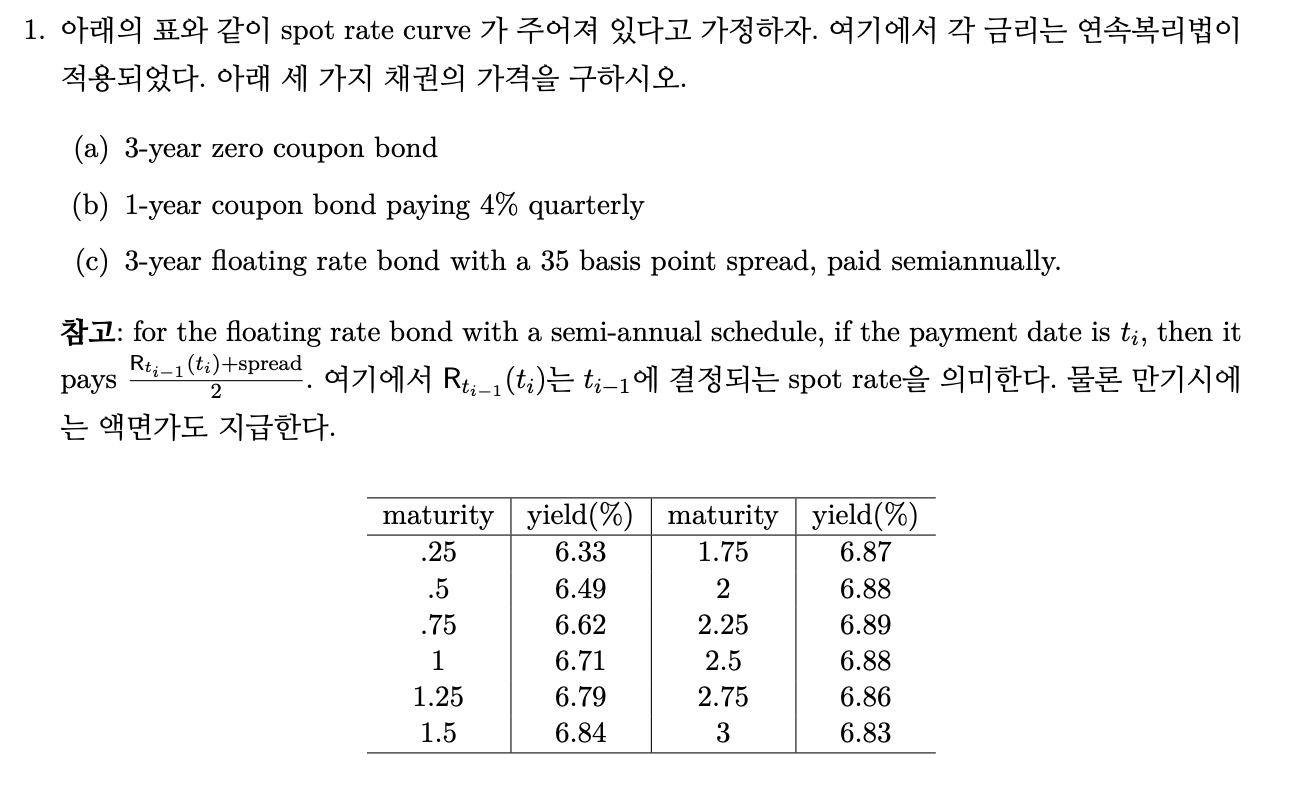
\includegraphics{images/이자율hw1_1.png}

\textbf{\emph{Answer}}

\begin{Shaded}
\begin{Highlighting}[]
\FunctionTok{rm}\NormalTok{(}\AttributeTok{list=}\FunctionTok{ls}\NormalTok{())}
\FunctionTok{library}\NormalTok{(tidyverse)}
\NormalTok{spot }\OtherTok{\textless{}{-}} \FunctionTok{tibble}\NormalTok{(}\AttributeTok{t=}\FunctionTok{seq}\NormalTok{(}\FloatTok{0.25}\NormalTok{,}\DecValTok{3}\NormalTok{,}\FloatTok{0.25}\NormalTok{), }
               \AttributeTok{y=}\FunctionTok{c}\NormalTok{(}\FloatTok{0.0633}\NormalTok{,}\FloatTok{0.0649}\NormalTok{,}\FloatTok{0.0662}\NormalTok{,}\FloatTok{0.0671}\NormalTok{,}\FloatTok{0.0679}\NormalTok{,}\FloatTok{0.0684}\NormalTok{,}
                   \FloatTok{0.0687}\NormalTok{,}\FloatTok{0.0688}\NormalTok{,}\FloatTok{0.0689}\NormalTok{,}\FloatTok{0.0688}\NormalTok{,}\FloatTok{0.0686}\NormalTok{,}\FloatTok{0.0683}\NormalTok{)) }\SpecialCharTok{\%\textgreater{}\%} 
  \FunctionTok{mutate}\NormalTok{(}\AttributeTok{d=}\FunctionTok{exp}\NormalTok{(}\SpecialCharTok{{-}}\NormalTok{y}\SpecialCharTok{*}\NormalTok{t))}
\end{Highlighting}
\end{Shaded}

\textbf{(a) 81.4729}

\begin{Shaded}
\begin{Highlighting}[]
\CommentTok{\# (a) 3{-}year zero coupon bond}
\NormalTok{a}\OtherTok{=}\DecValTok{100}\SpecialCharTok{*}\NormalTok{spot}\SpecialCharTok{$}\NormalTok{d[}\FunctionTok{which}\NormalTok{(spot}\SpecialCharTok{$}\NormalTok{t}\SpecialCharTok{==}\DecValTok{3}\NormalTok{)]}
\NormalTok{a}
\end{Highlighting}
\end{Shaded}

\begin{verbatim}
[1] 81.47288
\end{verbatim}

\textbf{(b) 97.3492}

\begin{Shaded}
\begin{Highlighting}[]
\NormalTok{b}\OtherTok{=}\NormalTok{spot }\SpecialCharTok{\%\textgreater{}\%}
  \FunctionTok{filter}\NormalTok{(t}\SpecialCharTok{\textless{}=}\DecValTok{1}\NormalTok{) }\SpecialCharTok{\%\textgreater{}\%} 
  \FunctionTok{mutate}\NormalTok{(}\AttributeTok{cf=}\FunctionTok{c}\NormalTok{(}\DecValTok{1}\NormalTok{,}\DecValTok{1}\NormalTok{,}\DecValTok{1}\NormalTok{,}\DecValTok{101}\NormalTok{)) }\SpecialCharTok{\%\textgreater{}\%} 
  \FunctionTok{mutate}\NormalTok{(}\AttributeTok{pv\_cf=}\NormalTok{cf}\SpecialCharTok{*}\NormalTok{d) }\SpecialCharTok{\%\textgreater{}\%} 
  \FunctionTok{select}\NormalTok{(pv\_cf) }\SpecialCharTok{\%\textgreater{}\%} 
  \FunctionTok{sum}\NormalTok{()}
\NormalTok{b}
\end{Highlighting}
\end{Shaded}

\begin{verbatim}
[1] 97.3492
\end{verbatim}

\textbf{(c) 100.9334}

FRN의 spread가 0이라면 가격은 액면가인 100에 거래될 것 입니다.

문제의 FRN은 35bp의 프리미엄을 지급하므로, FRN의 가격은
액면가+35bp쿠폰의 현재가치입니다.

\begin{Shaded}
\begin{Highlighting}[]
\CommentTok{\# (c) 3{-}year floating rate bond with a 35bp spread, semiannually}
\NormalTok{premium}\OtherTok{=}\NormalTok{spot }\SpecialCharTok{\%\textgreater{}\%}
  \FunctionTok{filter}\NormalTok{(t}\SpecialCharTok{\%\%}\FloatTok{0.5}\SpecialCharTok{==}\DecValTok{0}\NormalTok{) }\SpecialCharTok{\%\textgreater{}\%} 
  \FunctionTok{mutate}\NormalTok{(}\AttributeTok{cf=}\FunctionTok{rep}\NormalTok{(}\DecValTok{35}\SpecialCharTok{/}\DecValTok{10000}\SpecialCharTok{/}\DecValTok{2}\SpecialCharTok{*}\DecValTok{100}\NormalTok{,}\DecValTok{6}\NormalTok{)) }\SpecialCharTok{\%\textgreater{}\%} 
  \FunctionTok{mutate}\NormalTok{(}\AttributeTok{pv\_cf=}\NormalTok{cf}\SpecialCharTok{*}\NormalTok{d) }\SpecialCharTok{\%\textgreater{}\%} 
  \FunctionTok{select}\NormalTok{(pv\_cf) }\SpecialCharTok{\%\textgreater{}\%} 
  \FunctionTok{sum}\NormalTok{()}
\NormalTok{c}\OtherTok{=}\DecValTok{100}\SpecialCharTok{+}\NormalTok{premium}
\NormalTok{c}
\end{Highlighting}
\end{Shaded}

\begin{verbatim}
[1] 100.9334
\end{verbatim}

\subsection*{Problem2}\label{problem2}
\addcontentsline{toc}{subsection}{Problem2}

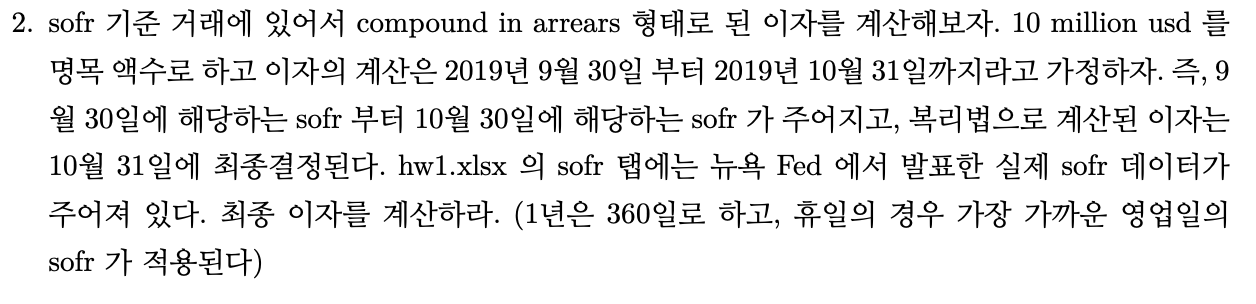
\includegraphics{images/이자율hw1_2.png}

\textbf{\emph{Answer}} : \textbf{16,187.27\$}

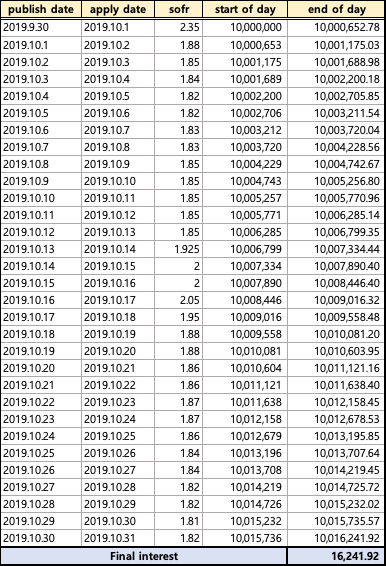
\includegraphics{images/이자율hw1_2_answer.png}

\subsection*{Problem3}\label{problem3}
\addcontentsline{toc}{subsection}{Problem3}


\includegraphics{images/이자율hw1_3.png}

\begin{quote}
증가하므로 / 감소하므로 / 상승하므로 / 하락하므로 / 거래이익이 /
거래손실이
\end{quote}

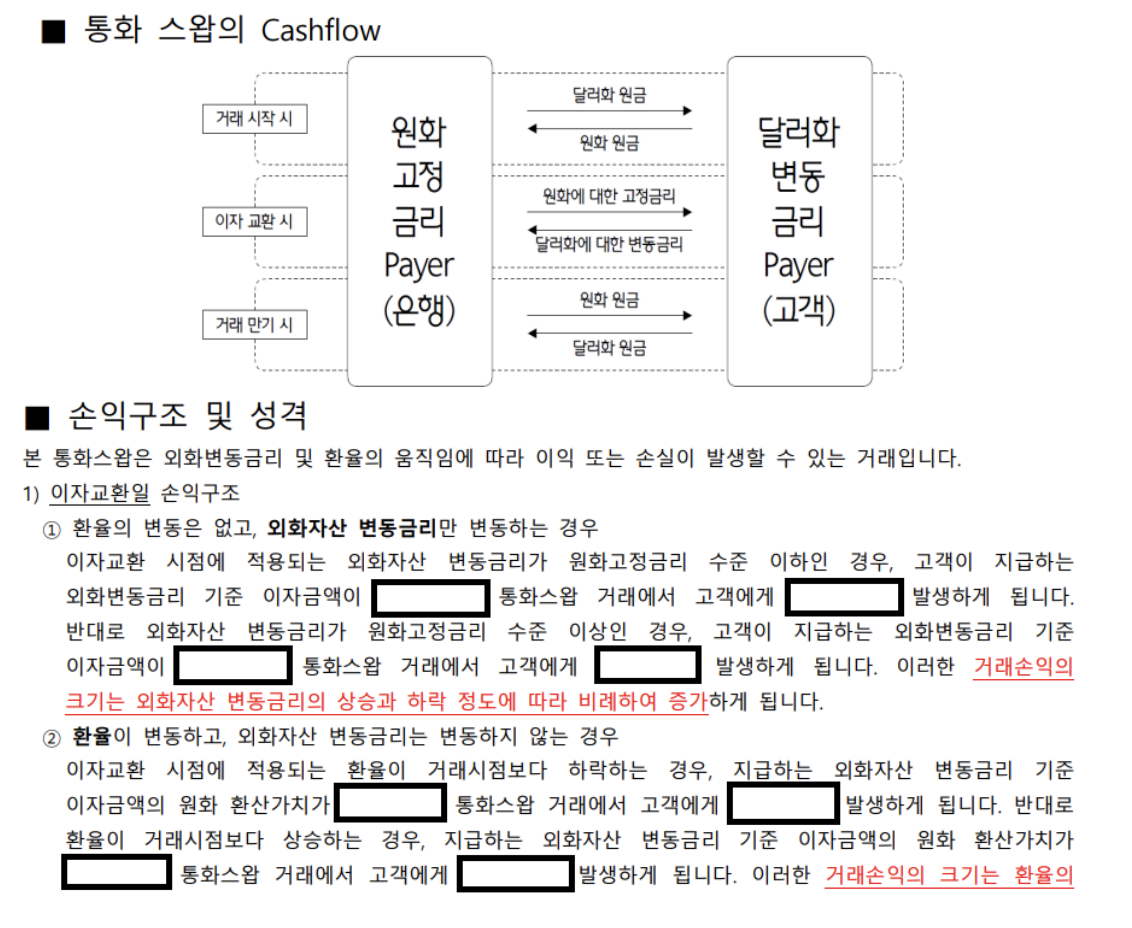
\includegraphics{images/이자율hw1_4.png}

\textbf{\emph{Answer}}

이자교환 시점에 적용되는 외화자산 변동금리가 원화고정금리 수준 이하인
경우, 고객이 지급하는 외화변동금리 기준 이자금액이
\textbf{\emph{감소하므로}} 통화스왑 거래에서 고객에게
\textbf{\emph{거래이익이}} 발생하게 됩니다. 반대로 외화자산 변동금리가
원화고정금리 수준 이상인 경우, 고객이 지급하는 외화변동금리 기준
이자금액이 \textbf{\emph{증가하므로}} 통화스왑 거래에서 고객에게
\textbf{\emph{거래손실이}} 발생하게 됩니다.

이자교환 시점에 적용되는 환율이 거래시점보다 하락하는 경우, 지급하는
외화자산 변동금리 기준 이자금액의 원화 환산가치가
\textbf{\emph{하락하므로}} 통화스왑 거래에서 고객에게
\textbf{\emph{거래이익이}} 발생하게 됩니다. 반대로 환율이 거래시점보다
상승하는 경우, 지급하는 외화자산 변동금리 기준 이자금액의 원화
환산가치가 \textbf{\emph{상승하므로}} 통화스왑 거래에서 고객에게
\textbf{\emph{거래손실이}} 발생하게 됩니다.

\subsection*{Problem4}\label{problem4}
\addcontentsline{toc}{subsection}{Problem4}

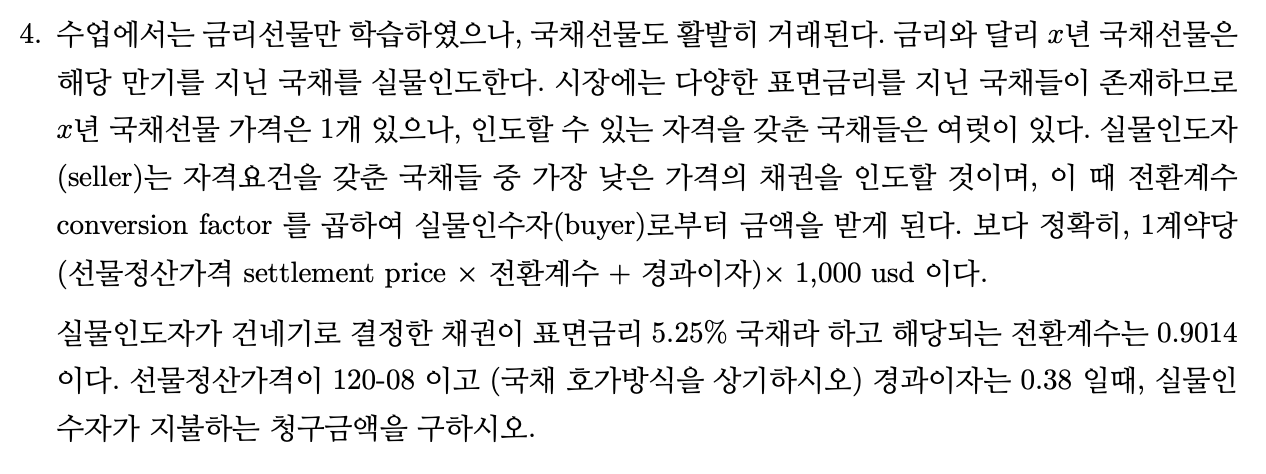
\includegraphics{images/이자율hw1_5.png}

\textbf{\emph{Answer}} : \textbf{108,773.3\$}

\begin{Shaded}
\begin{Highlighting}[]
\NormalTok{settle}\OtherTok{=}\DecValTok{120}\SpecialCharTok{+}\DecValTok{8}\SpecialCharTok{/}\DecValTok{32}
\NormalTok{cf}\OtherTok{=}\FloatTok{0.9014}
\NormalTok{accrued}\OtherTok{=}\FloatTok{0.38}

\NormalTok{value}\OtherTok{=}\NormalTok{(settle}\SpecialCharTok{*}\NormalTok{cf}\SpecialCharTok{+}\NormalTok{accrued)}\SpecialCharTok{*}\DecValTok{1000}
\NormalTok{value}
\end{Highlighting}
\end{Shaded}

\begin{verbatim}
[1] 108773.3
\end{verbatim}

\subsection*{Problem5}\label{problem5}
\addcontentsline{toc}{subsection}{Problem5}

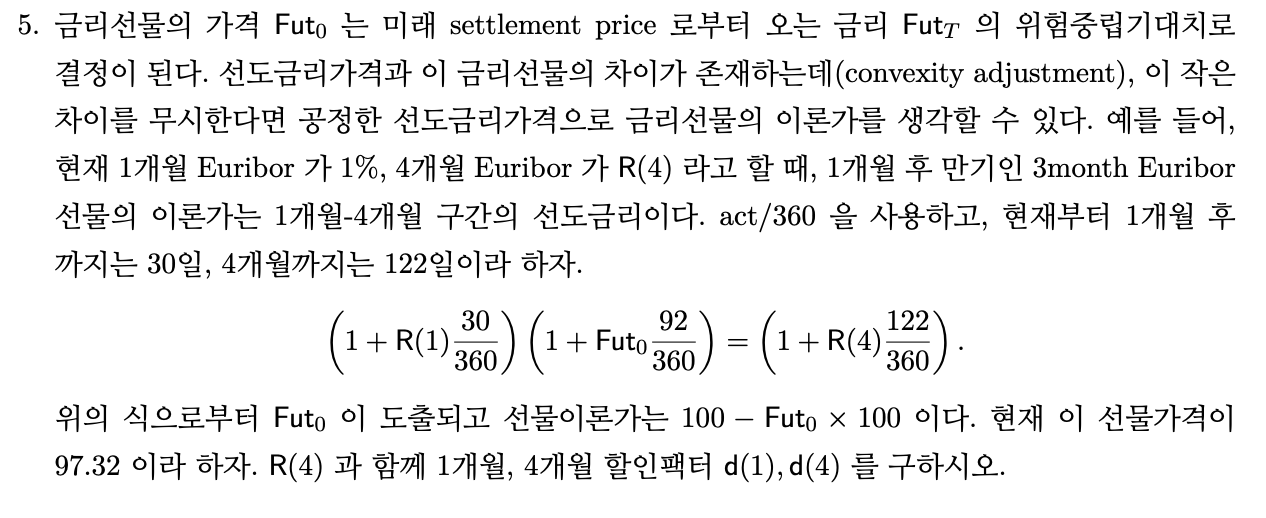
\includegraphics{images/이자율hw1_6.png}

\textbf{\emph{Answer}}

\(R(4)=2.2686\%,\;\;d(1)=0.9992,\;\;d(4)=0.9924\)

\begin{Shaded}
\begin{Highlighting}[]
\NormalTok{r1}\OtherTok{=}\FloatTok{0.01}
\NormalTok{theo\_prc}\OtherTok{=}\FloatTok{97.32}
\NormalTok{futures}\OtherTok{=}\NormalTok{(}\DecValTok{100}\SpecialCharTok{{-}}\NormalTok{theo\_prc)}\SpecialCharTok{/}\DecValTok{100}
\NormalTok{r4}\OtherTok{=}\NormalTok{((}\DecValTok{1}\SpecialCharTok{+}\NormalTok{r1}\SpecialCharTok{*}\DecValTok{30}\SpecialCharTok{/}\DecValTok{360}\NormalTok{)}\SpecialCharTok{*}\NormalTok{(}\DecValTok{1}\SpecialCharTok{+}\NormalTok{futures}\SpecialCharTok{*}\DecValTok{92}\SpecialCharTok{/}\DecValTok{360}\NormalTok{)}\SpecialCharTok{{-}}\DecValTok{1}\NormalTok{)}\SpecialCharTok{*}\DecValTok{360}\SpecialCharTok{/}\DecValTok{122}
\NormalTok{d1}\OtherTok{=}\DecValTok{1}\SpecialCharTok{/}\NormalTok{(}\DecValTok{1}\SpecialCharTok{+}\NormalTok{r1}\SpecialCharTok{*}\DecValTok{30}\SpecialCharTok{/}\DecValTok{360}\NormalTok{)}
\NormalTok{d4}\OtherTok{=}\DecValTok{1}\SpecialCharTok{/}\NormalTok{(}\DecValTok{1}\SpecialCharTok{+}\NormalTok{r4}\SpecialCharTok{*}\DecValTok{122}\SpecialCharTok{/}\DecValTok{360}\NormalTok{)}
\FunctionTok{paste}\NormalTok{(}\FunctionTok{round}\NormalTok{(r4,}\DecValTok{6}\NormalTok{),}\FunctionTok{round}\NormalTok{(d1,}\DecValTok{6}\NormalTok{),}\FunctionTok{round}\NormalTok{(d4,}\DecValTok{6}\NormalTok{),}\AttributeTok{sep=}\StringTok{" / "}\NormalTok{)}
\end{Highlighting}
\end{Shaded}

\begin{verbatim}
[1] "0.022686 / 0.999167 / 0.992371"
\end{verbatim}

\chapter*{이자율기간구조
과제2}\label{uxc774uxc790uxc728uxae30uxac04uxad6cuxc870-uxacfcuxc81c2}
\addcontentsline{toc}{chapter}{이자율기간구조 과제2}

\markboth{이자율기간구조 과제2}{이자율기간구조 과제2}

\section*{Problem 1}\label{problem-1-1}
\addcontentsline{toc}{section}{Problem 1}

\markright{Problem 1}

한 제조업체의 재무담당자가 usd 100 million 에 달하는 운전자본 working
capital 을 3개월 정도 repo 시장에 투자하여 이익을 취하고자 한다.

기간은 2020년 1월 15일(현재, 포함)에 시작하여 2020년 4월 15일(불포함)이
환매일이다. 즉 재무담당자는 91일 동안 daily SOFR 를 얻게 된다.

그러나 최근 SOFR 의 하락세가 고민이 되어 투자금의 절반인 50 million 은
2020년 4월 만기인 3개월 SOFR 선물을 매수하여 수익 금리를 고정하는 효과를
가지려고 한다.

기간 내내 금리가 1bp 하락한다면, act/360 기준으로 회사는 얼마의 손해가
발생하는가?

이 절반에 대하여 SOFR 선물로 헤지를 한다면 몇 개의 선물 계약을 해야할지
본인의 계산을 쓰세요.

\subsection*{Answer}\label{answer-5}
\addcontentsline{toc}{subsection}{Answer}

전체 노출액 중 절반은 정확히 헷지하였으므로, 기간 중 노출액은
50mUSD입니다.

노출기간은 91일이므로, \textbf{회사의 손해}는
\(50,000,000\times 0.0001\times\frac{91}{360}=1263.889USD\)

SOFR선물은 (100-r)로 호가하며, 1bp에 대해 25\$만큼 변동합니다.

따라서, 손실액만큼 SOFR선물에서 이익이 발생하도록 하려면
\(\frac{1263.889}{25}=50.56\), \textbf{약 51계약 매수}해야합니다.

\section*{Problem 2}\label{problem-2-1}
\addcontentsline{toc}{section}{Problem 2}

\markright{Problem 2}

다음의 표는 2020년 6월 5일 ICE에서 가져온 usd스왑데이터이다. 편의상 각
스왑금리는 연 1회 지급한다고 하자. 우리는 bootstrapping 기법을 이용하여
이 스왑금리들을 할인율곡선 또 는 현물이자율 곡선으로 변환할 수 있다.

이 문제에서는 그와 달리 매해 말 지급부담을 지니고 있는 은행 A를
고려한다. 이 은행은 현 시점에서 floating rate notes 변동금리부채권과
스왑을 매수하여 이 지급부담을 맞추려고 한다. 이때 변동금리부채권과
스왑의 액면값들을 구하는 것을 reverse bootstrapping 이라 한다. 보다
정확히 다음의 구조를 고려하자.

\begin{itemize}
\tightlist
\item
  각 FRN은 \(N_1, ... , N_6\)의 액면을 가지고 있으며 이들은 i번째 해의
  말까지 매년 \(N_i\) 에 해당하는 변동금리를 지급하고 i번째 해의 말에는
  액면 \(N_i\) 도 지급한다.
\item
  각 스왑의 액면 역시 \(N_i\)이며 A는 floating rate payer이다. 즉 i번째
  해의 말까지 매년 \(N_i\)에 해당하는 변동금리를 거래상대방에게
  지급한다. 역으로 거래상대방은 매해 말 \(N_is_i\) 을 지불한다. 여기에서
  \(s_i\)는 i 만기 스왑금리이다.
\end{itemize}

\(N_1,...,N_6\)를 구하고 소수점 네째자리까지 리포트하시오.

\begin{Shaded}
\begin{Highlighting}[]
\FunctionTok{library}\NormalTok{(tidyverse)}
\end{Highlighting}
\end{Shaded}

\begin{Shaded}
\begin{Highlighting}[]
\NormalTok{swap }\OtherTok{\textless{}{-}} \FunctionTok{tibble}\NormalTok{(}\AttributeTok{tenor=}\FunctionTok{c}\NormalTok{(}\DecValTok{1}\SpecialCharTok{:}\DecValTok{6}\NormalTok{),}
               \AttributeTok{rate=}\FunctionTok{c}\NormalTok{(}\FloatTok{0.307}\NormalTok{,}\FloatTok{0.299}\NormalTok{,}\FloatTok{0.346}\NormalTok{,}\FloatTok{0.424}\NormalTok{,}\FloatTok{0.517}\NormalTok{,}\FloatTok{0.614}\NormalTok{))}
\NormalTok{swap}
\end{Highlighting}
\end{Shaded}

\begin{verbatim}
# A tibble: 6 x 2
  tenor  rate
  <int> <dbl>
1     1 0.307
2     2 0.299
3     3 0.346
4     4 0.424
5     5 0.517
6     6 0.614
\end{verbatim}

\subsection*{Answer}\label{answer-6}
\addcontentsline{toc}{subsection}{Answer}

\section*{Problem 3}\label{problem-3-1}
\addcontentsline{toc}{section}{Problem 3}

\markright{Problem 3}

미 재무부에서 발표하는 일별 par yield 데이터를 찾되, 2024년 1월부터
5월까지 매월 첫번째 일자의 커브를 구하시오. 그리고 이 5개의 금리 커브에
대하여 Nelson-Siegel-Svensson 모형을 적용하여 본인이 구한 최선의 fitted
curve를 리포트하시오. 1개월 금리부터 30년 금리까지 데이터 전체를
활용하시오.

여기서 정답은 없으니, 본인이 적절한 초기값 및 제약식을 넣어 문제를
푸세요.

\subsection*{Answer}\label{answer-7}
\addcontentsline{toc}{subsection}{Answer}

먼저, \textbf{미 재무부의 daily par yield} 데이터를 이용하여 산출한 매월
첫번째 일자의 커브는 아래와 같습니다.

\begin{Shaded}
\begin{Highlighting}[]
\NormalTok{uspar }\OtherTok{\textless{}{-}} \FunctionTok{tibble}\NormalTok{()}
\NormalTok{uspar }\OtherTok{\textless{}{-}} \FunctionTok{read\_csv}\NormalTok{(}\StringTok{"investment\_hw/usparyield.csv"}\NormalTok{) }\SpecialCharTok{\%\textgreater{}\%} 
  \FunctionTok{arrange}\NormalTok{(Date) }\SpecialCharTok{\%\textgreater{}\%} 
  \FunctionTok{mutate}\NormalTok{(}\AttributeTok{year=}\FunctionTok{substr}\NormalTok{(Date,}\DecValTok{7}\NormalTok{,}\DecValTok{10}\NormalTok{),}
         \AttributeTok{month=}\FunctionTok{substr}\NormalTok{(Date,}\DecValTok{1}\NormalTok{,}\DecValTok{2}\NormalTok{)) }\SpecialCharTok{\%\textgreater{}\%} 
  \FunctionTok{group\_by}\NormalTok{(year,month) }\SpecialCharTok{\%\textgreater{}\%} 
  \FunctionTok{slice}\NormalTok{(}\DecValTok{1}\NormalTok{) }\SpecialCharTok{\%\textgreater{}\%} 
  \FunctionTok{pivot\_longer}\NormalTok{(}\AttributeTok{cols =} \FunctionTok{contains}\NormalTok{(}\StringTok{" "}\NormalTok{),}\AttributeTok{values\_to =} \StringTok{"par"}\NormalTok{, }\AttributeTok{names\_to =} \StringTok{"time"}\NormalTok{) }\SpecialCharTok{\%\textgreater{}\%} 
  \FunctionTok{mutate}\NormalTok{(}\AttributeTok{maturity=}\FunctionTok{c}\NormalTok{(}\DecValTok{1}\NormalTok{,}\DecValTok{2}\NormalTok{,}\DecValTok{3}\NormalTok{,}\DecValTok{4}\NormalTok{,}\DecValTok{6}\NormalTok{,}\DecValTok{12}\NormalTok{,}\DecValTok{24}\NormalTok{,}\DecValTok{36}\NormalTok{,}\DecValTok{60}\NormalTok{,}\DecValTok{84}\NormalTok{,}\DecValTok{120}\NormalTok{,}\DecValTok{240}\NormalTok{,}\DecValTok{360}\NormalTok{)}\SpecialCharTok{/}\DecValTok{12}\NormalTok{) }\SpecialCharTok{\%\textgreater{}\%} 
  \FunctionTok{ungroup}\NormalTok{()}
\end{Highlighting}
\end{Shaded}

\begin{Shaded}
\begin{Highlighting}[]
\FunctionTok{ggplot}\NormalTok{(uspar,}\FunctionTok{aes}\NormalTok{(}\AttributeTok{x=}\NormalTok{maturity,}\AttributeTok{y=}\NormalTok{par,}\AttributeTok{colour=}\NormalTok{month))}\SpecialCharTok{+}
  \FunctionTok{geom\_line}\NormalTok{()}\SpecialCharTok{+}
  \FunctionTok{theme\_bw}\NormalTok{()}
\end{Highlighting}
\end{Shaded}

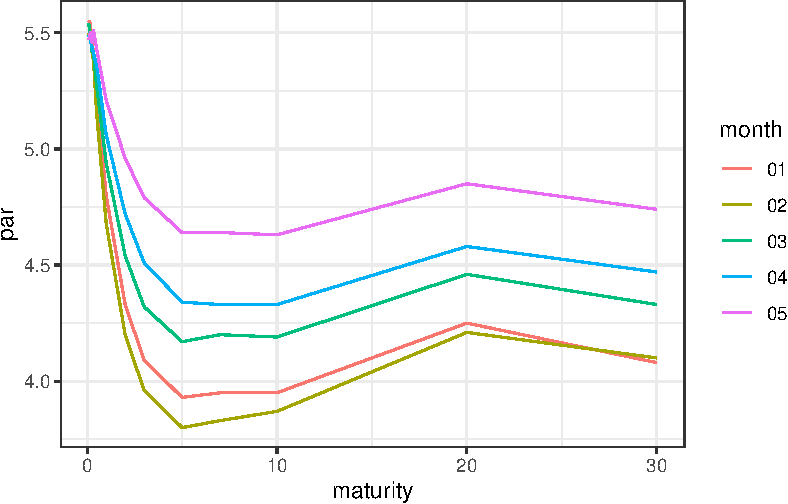
\includegraphics{이자율기간구조_hw2_files/figure-pdf/unnamed-chunk-4-1.pdf}

다음으로, \textbf{NSS모형을 이용한 최적 fitted curve}를 구해보겠습니다.

\begin{tcolorbox}[enhanced jigsaw, toprule=.15mm, colframe=quarto-callout-note-color-frame, opacitybacktitle=0.6, bottomtitle=1mm, left=2mm, breakable, coltitle=black, title=\textcolor{quarto-callout-note-color}{\faInfo}\hspace{0.5em}{Nelson-Siegel-Svensson Model}, colbacktitle=quarto-callout-note-color!10!white, opacityback=0, bottomrule=.15mm, toptitle=1mm, leftrule=.75mm, titlerule=0mm, colback=white, arc=.35mm, rightrule=.15mm]

NSS모형은 instantaneous forword rate를 추정하는 대표적인 모형으로, 3개의
factor와 6개의 parameter(\(\beta_0\sim\beta_3, \tau_1\sim\tau_2\))를
이용합니다.

\[f(t)=\beta_0+\beta_1e^{-\frac{t}{\tau_1}}+\beta_2\frac{t}{\tau_1}e^{-\frac{t}{\tau1}}+\beta_3\frac{t}{\tau_2}e^{-\frac{t}{\tau_2}}\]

이를 통해 continuous-compounding spot rate curve를 추정할 수 있습니다.

\[r(t)=\beta_0+\beta_1\frac{1-e^{-\frac{t}{\tau_1}}}{\frac{t}{\tau_1}}+\beta_2[\frac{1-e^{-\frac{t}{\tau_1}}}{\frac{t}{\tau_1}}-e^{-\frac{t}{\tau_1}}]+\beta_3[\frac{1-e^{-\frac{t}{\tau_2}}}{\frac{t}{\tau_2}}-e^{-\frac{t}{\tau_2}}]\]

\end{tcolorbox}

저는 \textbf{최적 fitted curve를 시뮬레이션을 통해 산출}할 예정입니다.

먼저, 초기값을
\(\beta_0=30y\;\;par\;\;rate,\;\;\;\beta_1=1m\;\;par\;\;rate-\beta_0\)
및 \(\beta_{2,3},\;\tau_{1,2}\)는 \((-5,\;5)\) 범위의 Uniform dist.
random number로 설정하겠습니다.

해당 초기값에 따라 constraint condition을 기준금리의 변동폭을 고려하여
25bp, \(|\beta_0+\beta_1-1m\;\;par\;\;rate|<0.25\)로 설정하고 finite
difference method(optim fn. in R)를 통해 최적해를 산출합니다. (tau와
beta는 별도의 제약식 없이 진행하였습니다.)

이러한 방식을 1,000번 반복하는 Monte-carlo simulation을 통해 1,000개의
최적해를 산출하고, 1,000개의 NSS rate curve에서 MSE가 가장 낮은 curve를
최적 fitted curve로 선정하겠습니다.

이를 구현하기 위한 \textbf{R코드 및 24년 1\textasciitilde5월의 fitted
curve는 아래와 같습니다.}

\subsubsection*{1. NSS Model 함수}\label{nss-model-uxd568uxc218}
\addcontentsline{toc}{subsubsection}{1. NSS Model 함수}

\begin{Shaded}
\begin{Highlighting}[]
\CommentTok{\# (nelson\_siegel) return NSS model rates for given parameters}
\CommentTok{\# maturity : vector of year maturity}
\CommentTok{\# params : vector of NSS medel 6 parameters, beta0 to tau2}

\NormalTok{nelson\_siegel }\OtherTok{\textless{}{-}} \ControlFlowTok{function}\NormalTok{(maturity, params)\{}
  
  \CommentTok{\# parameters }
\NormalTok{  beta0 }\OtherTok{=}\NormalTok{ params[}\DecValTok{1}\NormalTok{]}
\NormalTok{  beta1 }\OtherTok{=}\NormalTok{ params[}\DecValTok{2}\NormalTok{]}
\NormalTok{  beta2 }\OtherTok{=}\NormalTok{ params[}\DecValTok{3}\NormalTok{]}
\NormalTok{  beta3 }\OtherTok{=}\NormalTok{ params[}\DecValTok{4}\NormalTok{]}
\NormalTok{  tau1  }\OtherTok{=}\NormalTok{ params[}\DecValTok{5}\NormalTok{]}
\NormalTok{  tau2  }\OtherTok{=}\NormalTok{ params[}\DecValTok{6}\NormalTok{]}
  
  \CommentTok{\# function }
\NormalTok{  beta0 }\SpecialCharTok{+} 
\NormalTok{    beta1 }\SpecialCharTok{*}\NormalTok{ (}\DecValTok{1} \SpecialCharTok{{-}} \FunctionTok{exp}\NormalTok{(}\SpecialCharTok{{-}}\NormalTok{maturity}\SpecialCharTok{/}\NormalTok{tau1)) }\SpecialCharTok{/}\NormalTok{ (maturity}\SpecialCharTok{/}\NormalTok{tau1) }\SpecialCharTok{+} 
\NormalTok{    beta2 }\SpecialCharTok{*}\NormalTok{ ((}\DecValTok{1} \SpecialCharTok{{-}} \FunctionTok{exp}\NormalTok{(}\SpecialCharTok{{-}}\NormalTok{maturity}\SpecialCharTok{/}\NormalTok{tau1)) }\SpecialCharTok{/}\NormalTok{ (maturity}\SpecialCharTok{/}\NormalTok{tau1) }\SpecialCharTok{{-}} \FunctionTok{exp}\NormalTok{(}\SpecialCharTok{{-}}\NormalTok{maturity}\SpecialCharTok{/}\NormalTok{tau1)) }\SpecialCharTok{+} 
\NormalTok{    beta3 }\SpecialCharTok{*}\NormalTok{ ((}\DecValTok{1} \SpecialCharTok{{-}} \FunctionTok{exp}\NormalTok{(}\SpecialCharTok{{-}}\NormalTok{maturity}\SpecialCharTok{/}\NormalTok{tau2)) }\SpecialCharTok{/}\NormalTok{ (maturity}\SpecialCharTok{/}\NormalTok{tau2) }\SpecialCharTok{{-}} \FunctionTok{exp}\NormalTok{(}\SpecialCharTok{{-}}\NormalTok{maturity}\SpecialCharTok{/}\NormalTok{tau2)) }
  
\NormalTok{\}}
\end{Highlighting}
\end{Shaded}

\subsubsection*{2. NSS 최적해 산출 함수(finite difference
method)}\label{nss-uxcd5cuxc801uxd574-uxc0b0uxcd9c-uxd568uxc218finite-difference-method}
\addcontentsline{toc}{subsubsection}{2. NSS 최적해 산출 함수(finite
difference method)}

\begin{Shaded}
\begin{Highlighting}[]
\CommentTok{\# (optim\_nelson\_siegel) return optimal tibble for given term{-}structure,}
\CommentTok{\#                       using finite difference method}
\CommentTok{\# maturity : vector of year maturity}
\CommentTok{\# term\_sturucture : vector of real spot rate, order to maturity, omit \%}

\NormalTok{optim\_nelson\_siegel }\OtherTok{\textless{}{-}} \ControlFlowTok{function}\NormalTok{(}\AttributeTok{term\_structure =} \ConstantTok{NULL}\NormalTok{, }\AttributeTok{maturity =} \ConstantTok{NULL}\NormalTok{, }\AttributeTok{params =} \FunctionTok{rep}\NormalTok{(}\FloatTok{0.1}\NormalTok{, }\DecValTok{6}\NormalTok{),}
                                \AttributeTok{contraint\_threshold =} \FloatTok{0.1}\NormalTok{, }\AttributeTok{tau\_threshold =} \DecValTok{10}\NormalTok{, }\AttributeTok{beta\_threshold =} \DecValTok{30}\NormalTok{)\{}
  
\NormalTok{  loss\_function }\OtherTok{\textless{}{-}} \ControlFlowTok{function}\NormalTok{(params)\{}
    
    \CommentTok{\# parameters }
\NormalTok{    beta0 }\OtherTok{=}\NormalTok{ params[}\DecValTok{1}\NormalTok{]}
\NormalTok{    beta1 }\OtherTok{=}\NormalTok{ params[}\DecValTok{2}\NormalTok{]}
\NormalTok{    beta2 }\OtherTok{=}\NormalTok{ params[}\DecValTok{3}\NormalTok{]}
\NormalTok{    beta3 }\OtherTok{=}\NormalTok{ params[}\DecValTok{4}\NormalTok{]}
\NormalTok{    tau1  }\OtherTok{=}\NormalTok{ params[}\DecValTok{5}\NormalTok{]}
\NormalTok{    tau2  }\OtherTok{=}\NormalTok{ params[}\DecValTok{6}\NormalTok{]}
    
    \CommentTok{\# contraints}
\NormalTok{    contraint }\OtherTok{=} \FunctionTok{abs}\NormalTok{(beta0 }\SpecialCharTok{+}\NormalTok{ beta1 }\SpecialCharTok{{-}}\NormalTok{ term\_structure[}\DecValTok{1}\NormalTok{])}
    
    \ControlFlowTok{if}\NormalTok{(contraint }\SpecialCharTok{\textgreater{}}\NormalTok{ contraint\_threshold )\{}
      \FunctionTok{return}\NormalTok{(}\ConstantTok{NA}\NormalTok{)}
\NormalTok{    \}}
    
    \CommentTok{\# if(tau1 \textgreater{} tau\_threshold | tau2 \textgreater{} tau\_threshold)\{}
    \CommentTok{\#   return(NA)}
    \CommentTok{\# \}}
    \CommentTok{\# }
    \CommentTok{\# if(beta2 \textgreater{} beta\_threshold | beta3 \textgreater{} beta\_threshold )\{}
    \CommentTok{\#   return(NA)}
    \CommentTok{\# \}}
    
    \FunctionTok{sum}\NormalTok{(}
\NormalTok{      (term\_structure }\SpecialCharTok{{-}}\NormalTok{ beta0 }\SpecialCharTok{{-}} 
\NormalTok{         beta1 }\SpecialCharTok{*}\NormalTok{  (}\DecValTok{1} \SpecialCharTok{{-}} \FunctionTok{exp}\NormalTok{(}\SpecialCharTok{{-}}\NormalTok{maturity}\SpecialCharTok{/}\NormalTok{tau1)) }\SpecialCharTok{/}\NormalTok{ (maturity}\SpecialCharTok{/}\NormalTok{tau1) }\SpecialCharTok{{-}}
\NormalTok{         beta2 }\SpecialCharTok{*}\NormalTok{ ((}\DecValTok{1} \SpecialCharTok{{-}} \FunctionTok{exp}\NormalTok{(}\SpecialCharTok{{-}}\NormalTok{maturity}\SpecialCharTok{/}\NormalTok{tau1)) }\SpecialCharTok{/}\NormalTok{ (maturity}\SpecialCharTok{/}\NormalTok{tau1) }\SpecialCharTok{{-}} \FunctionTok{exp}\NormalTok{(}\SpecialCharTok{{-}}\NormalTok{maturity}\SpecialCharTok{/}\NormalTok{tau1)) }\SpecialCharTok{{-}} 
\NormalTok{         beta3 }\SpecialCharTok{*}\NormalTok{ ((}\DecValTok{1} \SpecialCharTok{{-}} \FunctionTok{exp}\NormalTok{(}\SpecialCharTok{{-}}\NormalTok{maturity}\SpecialCharTok{/}\NormalTok{tau2)) }\SpecialCharTok{/}\NormalTok{ (maturity}\SpecialCharTok{/}\NormalTok{tau2) }\SpecialCharTok{{-}} \FunctionTok{exp}\NormalTok{(}\SpecialCharTok{{-}}\NormalTok{maturity}\SpecialCharTok{/}\NormalTok{tau2)) }
\NormalTok{      )}\SpecialCharTok{\^{}}\DecValTok{2}\NormalTok{)}
    
\NormalTok{  \}}
  
  \CommentTok{\# set initial values for to beta0 and beta1 that respect the contraint }
  \CommentTok{\# beta0 is long{-}term rate \& beta1 is short{-}term rate minus beta0}
\NormalTok{  params }\OtherTok{=} \FunctionTok{c}\NormalTok{(term\_structure[}\FunctionTok{length}\NormalTok{(term\_structure)],}
\NormalTok{             term\_structure[}\DecValTok{1}\NormalTok{]}\SpecialCharTok{{-}}\NormalTok{term\_structure[}\FunctionTok{length}\NormalTok{(term\_structure)],}
\NormalTok{             params[}\DecValTok{3}\SpecialCharTok{:}\DecValTok{6}\NormalTok{] )}
               
  \CommentTok{\# beta0 \& beta1 is equal to (short{-}term rate)/2}
  \CommentTok{\# params = c(term\_structure[1]/2,term\_structure[1]/2,params[3:6] )}
  
  \CommentTok{\# minimization of the loss function }
\NormalTok{  optimization }\OtherTok{=} \FunctionTok{optim}\NormalTok{(params, loss\_function)}
  
  \CommentTok{\# optimal parameters }
\NormalTok{  optim\_params }\OtherTok{=} \FunctionTok{c}\NormalTok{(}\AttributeTok{beta0 =}\NormalTok{ optimization}\SpecialCharTok{$}\NormalTok{par[}\DecValTok{1}\NormalTok{], }
                   \AttributeTok{beta1 =}\NormalTok{ optimization}\SpecialCharTok{$}\NormalTok{par[}\DecValTok{2}\NormalTok{], }
                   \AttributeTok{beta2 =}\NormalTok{ optimization}\SpecialCharTok{$}\NormalTok{par[}\DecValTok{3}\NormalTok{],}
                   \AttributeTok{beta3 =}\NormalTok{ optimization}\SpecialCharTok{$}\NormalTok{par[}\DecValTok{4}\NormalTok{],}
                   \AttributeTok{tau1  =}\NormalTok{ optimization}\SpecialCharTok{$}\NormalTok{par[}\DecValTok{5}\NormalTok{], }
                   \AttributeTok{tau2  =}\NormalTok{ optimization}\SpecialCharTok{$}\NormalTok{par[}\DecValTok{6}\NormalTok{])}
  
  \CommentTok{\# fitted value from Nelson{-}Siegel base function }
\NormalTok{  fitted\_values }\OtherTok{=} \FunctionTok{nelson\_siegel}\NormalTok{(maturity, optim\_params)}
  
  \CommentTok{\# compute the mean square error}
\NormalTok{  mse\_fit }\OtherTok{=} \FunctionTok{sd}\NormalTok{(fitted\_values }\SpecialCharTok{{-}}\NormalTok{ term\_structure, }\AttributeTok{na.rm =} \ConstantTok{TRUE}\NormalTok{)}
  
  \CommentTok{\# output }
\NormalTok{  dplyr}\SpecialCharTok{::}\FunctionTok{tibble}\NormalTok{( }
    \AttributeTok{maturity =} \FunctionTok{list}\NormalTok{(maturity),}
    \AttributeTok{term\_structure =} \FunctionTok{list}\NormalTok{(term\_structure),}
    \AttributeTok{start\_params =} \FunctionTok{list}\NormalTok{(params),}
    \AttributeTok{optim\_params =} \FunctionTok{list}\NormalTok{(optim\_params),}
    \AttributeTok{fit =} \FunctionTok{list}\NormalTok{(fitted\_values),}
    \AttributeTok{mse =}\NormalTok{ mse\_fit}
\NormalTok{  )}
\NormalTok{\} }
\end{Highlighting}
\end{Shaded}

\subsubsection*{3. Uniform dist. random number
생성}\label{uniform-dist.-random-number-uxc0dduxc131}
\addcontentsline{toc}{subsubsection}{3. Uniform dist. random number
생성}

\begin{Shaded}
\begin{Highlighting}[]
\CommentTok{\# (random\_params) return random number follows an uniform distribution}
\CommentTok{\# n.params: number of parameter to generate }
\CommentTok{\# params.min: for random generation, minimum parameter}
\CommentTok{\# params.max: for random generation, maximum parameter}
\CommentTok{\# seed: to control randomness }

\NormalTok{random\_params }\OtherTok{\textless{}{-}} \ControlFlowTok{function}\NormalTok{(}\AttributeTok{n.params =} \DecValTok{1}\NormalTok{, }\AttributeTok{params.min =} \DecValTok{0}\NormalTok{, }\AttributeTok{params.max =} \DecValTok{5}\NormalTok{, }\AttributeTok{seed =} \DecValTok{1}\NormalTok{)\{}
  
  \FunctionTok{set.seed}\NormalTok{(seed)}
  
  \FunctionTok{runif}\NormalTok{(n.params, params.min, params.max)}
  
\NormalTok{\}}
\end{Highlighting}
\end{Shaded}

\subsubsection*{4. Monte-carlo simulation
(Calibration)}\label{monte-carlo-simulation-calibration}
\addcontentsline{toc}{subsubsection}{4. Monte-carlo simulation
(Calibration)}

\begin{Shaded}
\begin{Highlighting}[]
\CommentTok{\# (calibrate\_nelson\_siegel) return n{-}times "optim\_nelson\_siegel" outputs}
\CommentTok{\#                           using Monte{-}carlo simulation for random 3 parameters(beta2 to tau2)}
\CommentTok{\# n: number of simulations }
\CommentTok{\# params.min: for random generation, minimum parameter}
\CommentTok{\# params.max: for random generation, maximum parameter}
\CommentTok{\# verbose: disply progress in the importation.}

\NormalTok{calibrate\_nelson\_siegel }\OtherTok{\textless{}{-}} \ControlFlowTok{function}\NormalTok{(object, }\AttributeTok{n =} \DecValTok{100}\NormalTok{, }\AttributeTok{params.min =} \SpecialCharTok{{-}}\DecValTok{5}\NormalTok{, }\AttributeTok{params.max =} \DecValTok{5}\NormalTok{, }
                                    \AttributeTok{contraint\_threshold =} \FloatTok{0.01}\NormalTok{, }\AttributeTok{verbose =} \ConstantTok{TRUE}\NormalTok{ )\{}
  
  \CommentTok{\# initialize the parameters }
\NormalTok{  term\_structure }\OtherTok{=}\NormalTok{ object}\SpecialCharTok{$}\NormalTok{term\_structure[[}\DecValTok{1}\NormalTok{]]}
\NormalTok{  maturity }\OtherTok{=}\NormalTok{ object}\SpecialCharTok{$}\NormalTok{maturity[[}\DecValTok{1}\NormalTok{]]}
  
  \CommentTok{\# list containing all the simulations }
\NormalTok{  simulations }\OtherTok{=} \FunctionTok{list}\NormalTok{()}
  
  \CommentTok{\# safe version to avoid errors if we made many simulations}
\NormalTok{  safe\_optim }\OtherTok{=}\NormalTok{ purrr}\SpecialCharTok{::}\FunctionTok{safely}\NormalTok{(optim\_nelson\_siegel)}
  
  \ControlFlowTok{for}\NormalTok{(i }\ControlFlowTok{in} \DecValTok{1}\SpecialCharTok{:}\NormalTok{n)\{}
    
    \CommentTok{\# generate a random seed}
\NormalTok{    random\_seed }\OtherTok{=} \FunctionTok{mean}\NormalTok{(}\FunctionTok{random\_params}\NormalTok{(}\DecValTok{10}\NormalTok{, }\DecValTok{0}\NormalTok{, }\DecValTok{100000}\NormalTok{, }\AttributeTok{seed =}\NormalTok{ i))}
    
    \CommentTok{\# generate random parameters }
\NormalTok{    random\_params }\OtherTok{=} \FunctionTok{random\_params}\NormalTok{(}\DecValTok{6}\NormalTok{, params.min, params.max, }\AttributeTok{seed =}\NormalTok{ random\_seed)}
    
\NormalTok{    simulations[[i]] }\OtherTok{=} \FunctionTok{safe\_optim}\NormalTok{(}\AttributeTok{term\_structure  =}\NormalTok{ term\_structure, }\AttributeTok{maturity =}\NormalTok{ maturity, }\AttributeTok{params =}\NormalTok{ random\_params, }\AttributeTok{contraint\_threshold =}\NormalTok{ contraint\_threshold)}\SpecialCharTok{$}\NormalTok{result}
    
    \ControlFlowTok{if}\NormalTok{( verbose }\SpecialCharTok{\&}\NormalTok{(i}\SpecialCharTok{\%\%}\DecValTok{50} \SpecialCharTok{==} \DecValTok{0}\NormalTok{))\{}\FunctionTok{message}\NormalTok{(}\StringTok{"Simulations: "}\NormalTok{, i, }\StringTok{"/"}\NormalTok{, n)\}}
    
\NormalTok{  \}}
  
  \CommentTok{\# unique dataset for all the simulation}
\NormalTok{  simulations\_df }\OtherTok{=}\NormalTok{ dplyr}\SpecialCharTok{::}\FunctionTok{bind\_rows}\NormalTok{(simulations) }
  
  \CommentTok{\# add the initial object}
\NormalTok{  simulations\_df }\OtherTok{=}\NormalTok{ dplyr}\SpecialCharTok{::}\FunctionTok{bind\_rows}\NormalTok{(object, simulations) }
  
  \CommentTok{\# index for the simulations }
\NormalTok{  simulations\_df }\OtherTok{=}\NormalTok{ dplyr}\SpecialCharTok{::}\FunctionTok{mutate}\NormalTok{(simulations\_df, }\AttributeTok{n =} \DecValTok{1}\SpecialCharTok{:}\FunctionTok{nrow}\NormalTok{(simulations\_df)) }
  
  \FunctionTok{return}\NormalTok{(simulations\_df)}
  
\NormalTok{\}}
\end{Highlighting}
\end{Shaded}

\subsubsection*{5. Optimal fitted curve 산출 및
시각화}\label{optimal-fitted-curve-uxc0b0uxcd9c-uxbc0f-uxc2dcuxac01uxd654}
\addcontentsline{toc}{subsubsection}{5. Optimal fitted curve 산출 및
시각화}

\begin{Shaded}
\begin{Highlighting}[]
\CommentTok{\# (optimal\_params\_ns) summarize of all above, return optimal result minimize MSE from n{-}times simulation.}
\CommentTok{\# term\_structure = NULL}
\CommentTok{\# maturity = NULL}
\CommentTok{\# n = 1000}
\CommentTok{\# params.init = rep(0.1, 6)}
\CommentTok{\# params.min = {-}5}
\CommentTok{\# params.max = 5}
\CommentTok{\# contraint\_threshold = 0.1}
\CommentTok{\# label = NULL (label for the plot)}
\CommentTok{\# verbose = TRUE}

\NormalTok{optimal\_params\_ns }\OtherTok{\textless{}{-}} \ControlFlowTok{function}\NormalTok{(}\AttributeTok{term\_structure =} \ConstantTok{NULL}\NormalTok{, }\AttributeTok{maturity =} \ConstantTok{NULL}\NormalTok{, }
                              \AttributeTok{n =} \DecValTok{1000}\NormalTok{, }\AttributeTok{params.init =} \FunctionTok{rep}\NormalTok{(}\FloatTok{0.1}\NormalTok{, }\DecValTok{6}\NormalTok{), }\AttributeTok{params.min =} \SpecialCharTok{{-}}\DecValTok{5}\NormalTok{, }\AttributeTok{params.max =} \DecValTok{5}\NormalTok{,}
                              \AttributeTok{contraint\_threshold =} \FloatTok{0.1}\NormalTok{, }\AttributeTok{label =} \ConstantTok{NULL}\NormalTok{, }\AttributeTok{verbose =} \ConstantTok{TRUE}\NormalTok{)\{}
  
  \CommentTok{\# first fit }
\NormalTok{  first\_fit\_ns }\OtherTok{=} \FunctionTok{optim\_nelson\_siegel}\NormalTok{(}\AttributeTok{term\_structure =}\NormalTok{ term\_structure, }\AttributeTok{maturity =}\NormalTok{ maturity, }\AttributeTok{params =}\NormalTok{ params.init)}
  
  \CommentTok{\# simulations }
\NormalTok{  sim\_fit\_ns }\OtherTok{=} \FunctionTok{calibrate\_nelson\_siegel}\NormalTok{(first\_fit\_ns, }\AttributeTok{n =}\NormalTok{ n, }\AttributeTok{params.min =}\NormalTok{ params.min, }\AttributeTok{params.max =}\NormalTok{ params.max, }\AttributeTok{contraint\_threshold =}\NormalTok{ contraint\_threshold)}
  
  \CommentTok{\# best parameters }
\NormalTok{  df\_optim\_params }\OtherTok{=}\NormalTok{ sim\_fit\_ns[}\FunctionTok{which}\NormalTok{(sim\_fit\_ns}\SpecialCharTok{$}\NormalTok{mse }\SpecialCharTok{==} \FunctionTok{min}\NormalTok{(sim\_fit\_ns}\SpecialCharTok{$}\NormalTok{mse, }\AttributeTok{na.rm =} \ConstantTok{TRUE}\NormalTok{)),]}
  
  
  \CommentTok{\# setting the title of the plot }
  \ControlFlowTok{if}\NormalTok{(}\SpecialCharTok{!}\FunctionTok{is.null}\NormalTok{(label) }\SpecialCharTok{\&} \FunctionTok{is.character}\NormalTok{(label))\{}
    
\NormalTok{    plot\_title }\OtherTok{=} \FunctionTok{paste0}\NormalTok{(}\StringTok{"Fitted Nelson{-}Siegel{-}Svensonn vs Real Value "}\NormalTok{, }\StringTok{"("}\NormalTok{, label, }\StringTok{")"}\NormalTok{ )}
    
\NormalTok{  \} }\ControlFlowTok{else}\NormalTok{ \{}
    
\NormalTok{    plot\_title }\OtherTok{=} \StringTok{"Fitted Nelson{-}Siegel{-}Svensonn vs Real Value"}
\NormalTok{  \}}
  
  
  \CommentTok{\# plot of fitted vs real values }
\NormalTok{  plot\_df }\OtherTok{=}\NormalTok{  dplyr}\SpecialCharTok{::}\FunctionTok{inner\_join}\NormalTok{(}
\NormalTok{    dplyr}\SpecialCharTok{::}\FunctionTok{tibble}\NormalTok{(}
      \AttributeTok{t =}\NormalTok{ maturity,}
      \AttributeTok{pred =}\NormalTok{ df\_optim\_params}\SpecialCharTok{$}\NormalTok{fit[[}\DecValTok{1}\NormalTok{]]}
\NormalTok{    ),}
\NormalTok{    dplyr}\SpecialCharTok{::}\FunctionTok{tibble}\NormalTok{(}
      \AttributeTok{t =}\NormalTok{ maturity,}
      \AttributeTok{real =}\NormalTok{ term\_structure}
\NormalTok{    ),}
    \AttributeTok{by =} \StringTok{"t"}
\NormalTok{  ) }
  
  \CommentTok{\# Plot Real value vs Fitted Values }
\NormalTok{  plot\_ns }\OtherTok{=}\NormalTok{ plot\_df }\SpecialCharTok{\%\textgreater{}\%}
    \FunctionTok{mutate}\NormalTok{(}\AttributeTok{label =} \FunctionTok{paste0}\NormalTok{(}\StringTok{"T = "}\NormalTok{, }\FunctionTok{round}\NormalTok{(t, }\DecValTok{3}\NormalTok{)))}\SpecialCharTok{\%\textgreater{}\%}
    \FunctionTok{ggplot}\NormalTok{()}\SpecialCharTok{+}
    \FunctionTok{geom\_point}\NormalTok{(}\FunctionTok{aes}\NormalTok{(t, pred), }\AttributeTok{color =} \StringTok{"red"}\NormalTok{, }\AttributeTok{size =} \DecValTok{2}\NormalTok{, }\AttributeTok{alpha =} \FloatTok{0.8}\NormalTok{) }\SpecialCharTok{+}
    \FunctionTok{geom\_point}\NormalTok{(}\FunctionTok{aes}\NormalTok{(t, real), }\AttributeTok{color =} \StringTok{"black"}\NormalTok{, }\AttributeTok{alpha =} \FloatTok{0.5}\NormalTok{)}\SpecialCharTok{+}
    \FunctionTok{geom\_line}\NormalTok{(}\FunctionTok{aes}\NormalTok{(t, pred), }\AttributeTok{color =} \StringTok{"red"}\NormalTok{, }\AttributeTok{size =} \DecValTok{1}\NormalTok{) }\SpecialCharTok{+}
    \FunctionTok{geom\_line}\NormalTok{(}\FunctionTok{aes}\NormalTok{(t, real), }\AttributeTok{color =} \StringTok{"black"}\NormalTok{, }\AttributeTok{linetype =} \StringTok{"dashed"}\NormalTok{) }\SpecialCharTok{+}
    \FunctionTok{geom\_label}\NormalTok{(}\FunctionTok{aes}\NormalTok{(t}\SpecialCharTok{+}\DecValTok{1}\NormalTok{, real}\FloatTok{{-}0.001}\NormalTok{, }\AttributeTok{label =}\NormalTok{ label), }\AttributeTok{size =} \FloatTok{1.5}\NormalTok{)}\SpecialCharTok{+}
    \FunctionTok{theme}\NormalTok{(}\AttributeTok{axis.text.x =} \FunctionTok{element\_text}\NormalTok{(}\AttributeTok{angle =} \DecValTok{25}\NormalTok{, }\AttributeTok{face =} \StringTok{"bold"}\NormalTok{, }\AttributeTok{size =} \DecValTok{7}\NormalTok{), }
          \AttributeTok{axis.text.y =} \FunctionTok{element\_text}\NormalTok{(}\AttributeTok{face =} \StringTok{"bold"}\NormalTok{), }
          \AttributeTok{axis.title  =} \FunctionTok{element\_text}\NormalTok{(}\AttributeTok{face =} \StringTok{"bold"}\NormalTok{),}
          \AttributeTok{plot.title  =} \FunctionTok{element\_text}\NormalTok{(}\AttributeTok{face =} \StringTok{"bold"}\NormalTok{),}
          \AttributeTok{plot.subtitle =} \FunctionTok{element\_text}\NormalTok{(}\AttributeTok{face =} \StringTok{"italic"}\NormalTok{),}
          \AttributeTok{plot.caption =} \FunctionTok{element\_text}\NormalTok{(}\AttributeTok{face =} \StringTok{"italic"}\NormalTok{),}
          \AttributeTok{panel.grid.major.x =} \FunctionTok{element\_line}\NormalTok{(}\AttributeTok{colour=}\StringTok{"grey60"}\NormalTok{, }\AttributeTok{linetype=}\StringTok{"dotted"}\NormalTok{),}
          \AttributeTok{panel.grid.minor.x =} \FunctionTok{element\_blank}\NormalTok{(),}
          \AttributeTok{panel.grid.major.y =} \FunctionTok{element\_line}\NormalTok{(}\AttributeTok{colour=}\StringTok{"grey60"}\NormalTok{, }\AttributeTok{linetype=}\StringTok{"dotted"}\NormalTok{),}
          \AttributeTok{legend.text =} \FunctionTok{element\_text}\NormalTok{(}\AttributeTok{face =} \StringTok{"italic"}\NormalTok{, }\AttributeTok{size =} \DecValTok{5}\NormalTok{),}
          \AttributeTok{legend.title =} \FunctionTok{element\_text}\NormalTok{(}\AttributeTok{face =} \StringTok{"bold"}\NormalTok{),}
          \AttributeTok{legend.position =} \StringTok{"top"}\NormalTok{ ) }\SpecialCharTok{+}
    \FunctionTok{scale\_x\_continuous}\NormalTok{(}\AttributeTok{breaks=}\FunctionTok{c}\NormalTok{(}\DecValTok{0}\NormalTok{, }\FloatTok{0.5}\NormalTok{, }\DecValTok{1}\NormalTok{,}\DecValTok{2}\NormalTok{,}\DecValTok{3}\NormalTok{,}\DecValTok{4}\NormalTok{,}\DecValTok{5}\NormalTok{,}\DecValTok{7}\NormalTok{,}\DecValTok{10}\NormalTok{,}\DecValTok{15}\NormalTok{, }\DecValTok{20}\NormalTok{, }\DecValTok{25}\NormalTok{, }\DecValTok{30}\NormalTok{))}\SpecialCharTok{+}
    \FunctionTok{ggtitle}\NormalTok{(plot\_title, }\AttributeTok{subtitle =} \StringTok{"Fitted Value in Red and Real Values in Black"}\NormalTok{ )}\SpecialCharTok{+}
    \FunctionTok{xlab}\NormalTok{(}\StringTok{"Maturities"}\NormalTok{)}\SpecialCharTok{+}
    \FunctionTok{ylab}\NormalTok{(}\StringTok{""}\NormalTok{) }\SpecialCharTok{+} 
    \FunctionTok{labs}\NormalTok{(}\AttributeTok{caption =} \FunctionTok{paste0}\NormalTok{(}\StringTok{"Mean Squared Error of the Fit: "}\NormalTok{, }\FunctionTok{round}\NormalTok{(df\_optim\_params}\SpecialCharTok{$}\NormalTok{mse, }\DecValTok{6}\NormalTok{)))}\SpecialCharTok{+}
    \FunctionTok{theme\_bw}\NormalTok{()}
  
  
  
  \CommentTok{\# output }
  \FunctionTok{structure}\NormalTok{(}
    \FunctionTok{list}\NormalTok{(}
      \AttributeTok{optim\_params =} \FunctionTok{tibble}\NormalTok{( }\AttributeTok{beta0=}\NormalTok{df\_optim\_params}\SpecialCharTok{$}\NormalTok{optim\_params[[}\DecValTok{1}\NormalTok{]][}\DecValTok{1}\NormalTok{],}
                             \AttributeTok{beta1=}\NormalTok{df\_optim\_params}\SpecialCharTok{$}\NormalTok{optim\_params[[}\DecValTok{1}\NormalTok{]][}\DecValTok{2}\NormalTok{],}
                             \AttributeTok{beta2=}\NormalTok{df\_optim\_params}\SpecialCharTok{$}\NormalTok{optim\_params[[}\DecValTok{1}\NormalTok{]][}\DecValTok{3}\NormalTok{],}
                             \AttributeTok{beta3=}\NormalTok{df\_optim\_params}\SpecialCharTok{$}\NormalTok{optim\_params[[}\DecValTok{1}\NormalTok{]][}\DecValTok{4}\NormalTok{],}
                             \AttributeTok{tau1=}\NormalTok{df\_optim\_params}\SpecialCharTok{$}\NormalTok{optim\_params[[}\DecValTok{1}\NormalTok{]][}\DecValTok{5}\NormalTok{],}
                             \AttributeTok{tau2=}\NormalTok{df\_optim\_params}\SpecialCharTok{$}\NormalTok{optim\_params[[}\DecValTok{1}\NormalTok{]][}\DecValTok{6}\NormalTok{]),}
      \AttributeTok{plot\_ns =}\NormalTok{ plot\_ns,}
      \AttributeTok{simulations =}\NormalTok{ sim\_fit\_ns,}
      \AttributeTok{df\_optim =}\NormalTok{ df\_optim\_params}
      
\NormalTok{    )}
\NormalTok{  )}
  
\NormalTok{\}}
\end{Highlighting}
\end{Shaded}

\subsubsection*{Result}\label{result}
\addcontentsline{toc}{subsubsection}{Result}

앞서 도식화한 \textbf{24년 1\textasciitilde5월의 US par-yield curve}에
위 방법을 적용하여 \textbf{각각 모델링한 fitted curve는 아래와
같습니다.}

\begin{Shaded}
\begin{Highlighting}[]
\NormalTok{uspar\_jan }\OtherTok{\textless{}{-}}\NormalTok{ uspar }\SpecialCharTok{\%\textgreater{}\%} \FunctionTok{filter}\NormalTok{(month}\SpecialCharTok{==}\StringTok{"01"}\NormalTok{)}
\NormalTok{uspar\_feb }\OtherTok{\textless{}{-}}\NormalTok{ uspar }\SpecialCharTok{\%\textgreater{}\%} \FunctionTok{filter}\NormalTok{(month}\SpecialCharTok{==}\StringTok{"02"}\NormalTok{)}
\NormalTok{uspar\_mar }\OtherTok{\textless{}{-}}\NormalTok{ uspar }\SpecialCharTok{\%\textgreater{}\%} \FunctionTok{filter}\NormalTok{(month}\SpecialCharTok{==}\StringTok{"03"}\NormalTok{)}
\NormalTok{uspar\_apr }\OtherTok{\textless{}{-}}\NormalTok{ uspar }\SpecialCharTok{\%\textgreater{}\%} \FunctionTok{filter}\NormalTok{(month}\SpecialCharTok{==}\StringTok{"04"}\NormalTok{)}
\NormalTok{uspar\_may }\OtherTok{\textless{}{-}}\NormalTok{ uspar }\SpecialCharTok{\%\textgreater{}\%} \FunctionTok{filter}\NormalTok{(month}\SpecialCharTok{==}\StringTok{"05"}\NormalTok{)}

\NormalTok{Jan }\OtherTok{\textless{}{-}} \FunctionTok{optimal\_params\_ns}\NormalTok{(uspar\_jan}\SpecialCharTok{$}\NormalTok{par,uspar\_jan}\SpecialCharTok{$}\NormalTok{maturity,}\AttributeTok{n=}\DecValTok{1000}\NormalTok{,}\AttributeTok{contraint\_threshold =} \FloatTok{0.25}\NormalTok{)}
\NormalTok{Feb }\OtherTok{\textless{}{-}} \FunctionTok{optimal\_params\_ns}\NormalTok{(uspar\_feb}\SpecialCharTok{$}\NormalTok{par,uspar\_feb}\SpecialCharTok{$}\NormalTok{maturity,}\AttributeTok{n=}\DecValTok{1000}\NormalTok{,}\AttributeTok{contraint\_threshold =} \FloatTok{0.25}\NormalTok{)}
\NormalTok{Mar }\OtherTok{\textless{}{-}} \FunctionTok{optimal\_params\_ns}\NormalTok{(uspar\_mar}\SpecialCharTok{$}\NormalTok{par,uspar\_mar}\SpecialCharTok{$}\NormalTok{maturity,}\AttributeTok{n=}\DecValTok{1000}\NormalTok{,}\AttributeTok{contraint\_threshold =} \FloatTok{0.25}\NormalTok{)}
\NormalTok{Apr }\OtherTok{\textless{}{-}} \FunctionTok{optimal\_params\_ns}\NormalTok{(uspar\_apr}\SpecialCharTok{$}\NormalTok{par,uspar\_apr}\SpecialCharTok{$}\NormalTok{maturity,}\AttributeTok{n=}\DecValTok{1000}\NormalTok{,}\AttributeTok{contraint\_threshold =} \FloatTok{0.25}\NormalTok{)}
\NormalTok{May }\OtherTok{\textless{}{-}} \FunctionTok{optimal\_params\_ns}\NormalTok{(uspar\_may}\SpecialCharTok{$}\NormalTok{par,uspar\_may}\SpecialCharTok{$}\NormalTok{maturity,}\AttributeTok{n=}\DecValTok{1000}\NormalTok{,}\AttributeTok{contraint\_threshold =} \FloatTok{0.25}\NormalTok{)}
\end{Highlighting}
\end{Shaded}

\begin{Shaded}
\begin{Highlighting}[]
\NormalTok{Jan}\SpecialCharTok{$}\NormalTok{plot\_ns}
\end{Highlighting}
\end{Shaded}

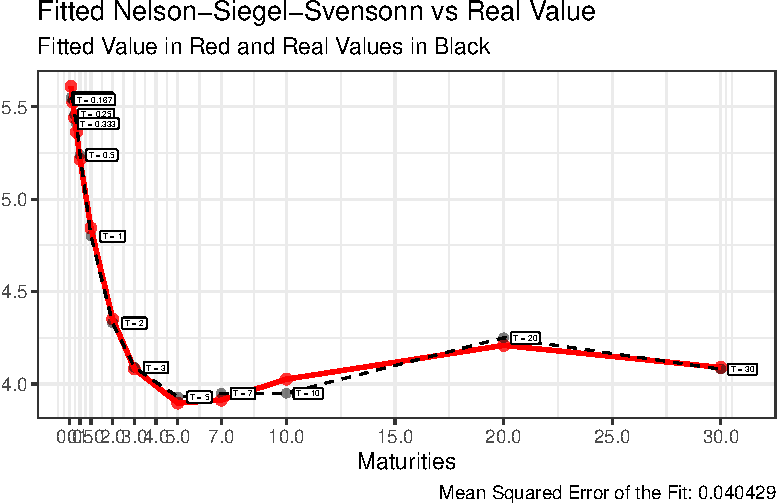
\includegraphics{이자율기간구조_hw2_files/figure-pdf/unnamed-chunk-11-1.pdf}

\begin{Shaded}
\begin{Highlighting}[]
\NormalTok{Feb}\SpecialCharTok{$}\NormalTok{plot\_ns}
\end{Highlighting}
\end{Shaded}

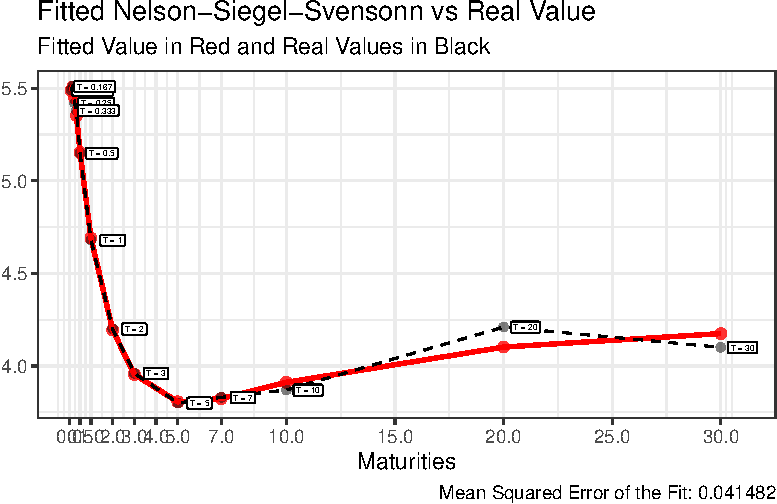
\includegraphics{이자율기간구조_hw2_files/figure-pdf/unnamed-chunk-11-2.pdf}

\begin{Shaded}
\begin{Highlighting}[]
\NormalTok{Mar}\SpecialCharTok{$}\NormalTok{plot\_ns}
\end{Highlighting}
\end{Shaded}

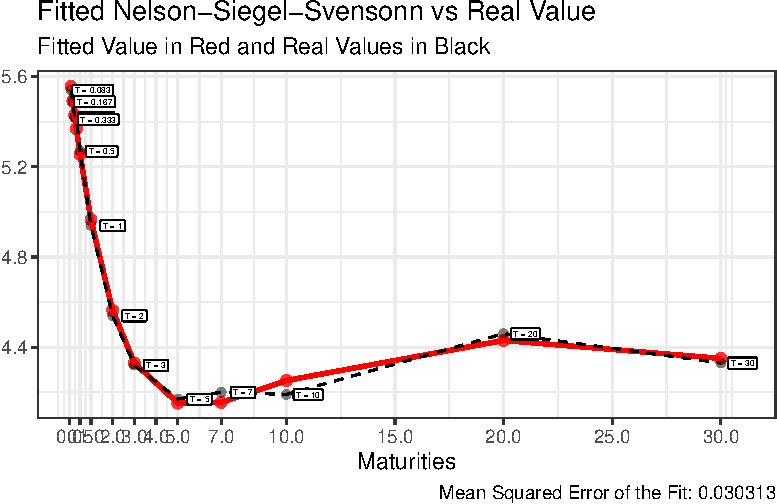
\includegraphics{이자율기간구조_hw2_files/figure-pdf/unnamed-chunk-11-3.pdf}

\begin{Shaded}
\begin{Highlighting}[]
\NormalTok{Apr}\SpecialCharTok{$}\NormalTok{plot\_ns}
\end{Highlighting}
\end{Shaded}

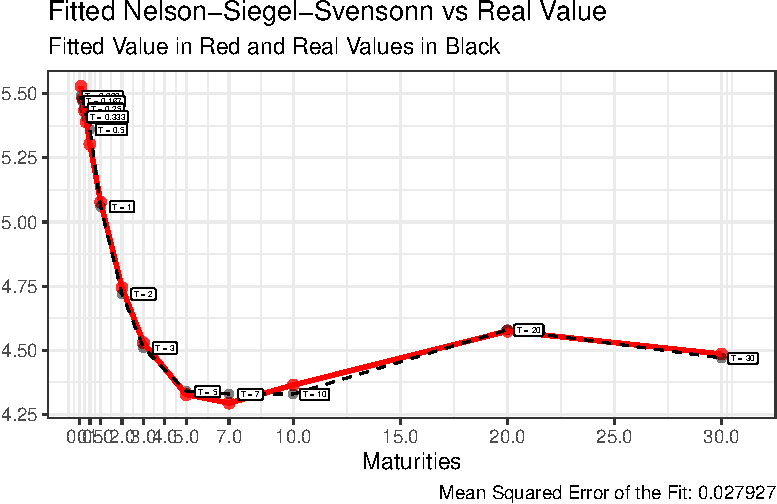
\includegraphics{이자율기간구조_hw2_files/figure-pdf/unnamed-chunk-11-4.pdf}

\begin{Shaded}
\begin{Highlighting}[]
\NormalTok{May}\SpecialCharTok{$}\NormalTok{plot\_ns}
\end{Highlighting}
\end{Shaded}

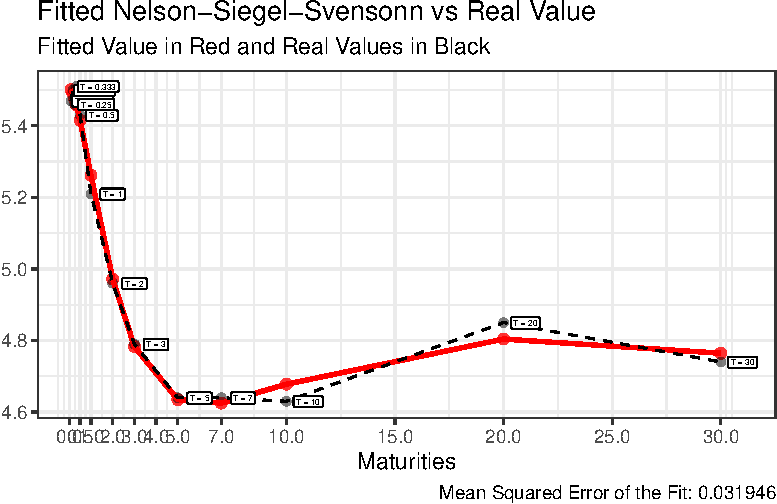
\includegraphics{이자율기간구조_hw2_files/figure-pdf/unnamed-chunk-11-5.pdf}

\section*{Problem 4}\label{problem-4}
\addcontentsline{toc}{section}{Problem 4}

\markright{Problem 4}

위 문제에서 구한 모수값들을 가지고 6월 첫날의 금리커브를 예측하려고
한다. 모수값들에 대하여 적절한 (예: 엑셀에서 제공하는 선형 추세선을 찾아
사용) 예측값들을 구하고 이를 바탕으로 금리 커브를 구하시오.

\subsection*{Answer}\label{answer-8}
\addcontentsline{toc}{subsection}{Answer}

먼저, 문제3에서 최종적으로 산출한 NSS fitted curve에 대하여 각각의
파라미터는 아래와 같습니다.

\begin{Shaded}
\begin{Highlighting}[]
\NormalTok{optim\_parameters }\OtherTok{\textless{}{-}}\NormalTok{ Jan}\SpecialCharTok{$}\NormalTok{optim\_params }\SpecialCharTok{\%\textgreater{}\%} 
  \FunctionTok{union\_all}\NormalTok{(Feb}\SpecialCharTok{$}\NormalTok{optim\_params) }\SpecialCharTok{\%\textgreater{}\%} 
  \FunctionTok{union\_all}\NormalTok{(Mar}\SpecialCharTok{$}\NormalTok{optim\_params) }\SpecialCharTok{\%\textgreater{}\%} 
  \FunctionTok{union\_all}\NormalTok{(Apr}\SpecialCharTok{$}\NormalTok{optim\_params) }\SpecialCharTok{\%\textgreater{}\%} 
  \FunctionTok{union\_all}\NormalTok{(May}\SpecialCharTok{$}\NormalTok{optim\_params) }\SpecialCharTok{\%\textgreater{}\%} 
  \FunctionTok{mutate}\NormalTok{(}\AttributeTok{month=}\FunctionTok{c}\NormalTok{(}\StringTok{"Jan"}\NormalTok{,}\StringTok{"Feb"}\NormalTok{,}\StringTok{"Mar"}\NormalTok{,}\StringTok{"Apr"}\NormalTok{,}\StringTok{"May"}\NormalTok{))}
\NormalTok{optim\_parameters}
\end{Highlighting}
\end{Shaded}

\begin{verbatim}
# A tibble: 5 x 7
  beta0 beta1 beta2 beta3  tau1   tau2 month
  <dbl> <dbl> <dbl> <dbl> <dbl>  <dbl> <chr>
1  2.35 3.35  -2.33  5.88 2.10  11.8   Jan  
2  4.32 0.961 -3.16  1.34 2.06   0.127 Feb  
3  3.32 2.30  -3.09  4.07 2.63  10.3   Mar  
4  2.69 2.89  -3.15  6.44 3.45  11.7   Apr  
5  3.46 2.05   1.74  4.09 0.802 14.1   May  
\end{verbatim}

이를 이용하여 6월달의 US par-yield curve를 예측하고자 할 때, 모수값들을
활용하여 NSS모델의 6월 예상파라미터를 추정할 수 있습니다.

여기에는 AR, ARMA, GARCH 등의 여러 모델을 생각할 수 있겠으나, 저는 직전
달의 모수값이 다음 달의 모수값에 대한 최적 추정치라고 생각합니다.
모수값의 시계열자료가 5개에 불과하고, \textbf{특별한 선형관계나 추세가
관찰되지 않기 때문}입니다. 이에 따라 \textbf{5월달의 NSS모델의 모수값을
6월의 예상파라미터}로 고려하겠습니다.

이를 이용하여 산출한** 6월 예상 US par-yield 및 curve는 아래와
같습니다.**

\begin{Shaded}
\begin{Highlighting}[]
\NormalTok{est\_jun }\OtherTok{\textless{}{-}} \FunctionTok{tibble}\NormalTok{(}\AttributeTok{maturity=}\NormalTok{uspar\_may}\SpecialCharTok{$}\NormalTok{maturity,}
                  \AttributeTok{par=}\NormalTok{May}\SpecialCharTok{$}\NormalTok{df\_optim}\SpecialCharTok{$}\NormalTok{fit[[}\DecValTok{1}\NormalTok{]])}
\NormalTok{est\_jun}
\end{Highlighting}
\end{Shaded}

\begin{verbatim}
# A tibble: 13 x 2
   maturity   par
      <dbl> <dbl>
 1   0.0833  5.50
 2   0.167   5.49
 3   0.25    5.48
 4   0.333   5.46
 5   0.5     5.42
 6   1       5.26
 7   2       4.97
 8   3       4.78
 9   5       4.63
10   7       4.62
11  10       4.68
12  20       4.80
13  30       4.76
\end{verbatim}

\begin{Shaded}
\begin{Highlighting}[]
\FunctionTok{ggplot}\NormalTok{(est\_jun,}\FunctionTok{aes}\NormalTok{(}\AttributeTok{x=}\NormalTok{maturity,}\AttributeTok{y=}\NormalTok{par))}\SpecialCharTok{+}
  \FunctionTok{geom\_line}\NormalTok{(}\AttributeTok{colour=}\StringTok{"blue"}\NormalTok{, }\AttributeTok{size=}\DecValTok{1}\NormalTok{)}\SpecialCharTok{+}
  \FunctionTok{scale\_x\_continuous}\NormalTok{(}\AttributeTok{breaks=}\FunctionTok{c}\NormalTok{(}\DecValTok{0}\NormalTok{, }\FloatTok{0.5}\NormalTok{, }\DecValTok{1}\NormalTok{,}\DecValTok{2}\NormalTok{,}\DecValTok{3}\NormalTok{,}\DecValTok{4}\NormalTok{,}\DecValTok{5}\NormalTok{,}\DecValTok{7}\NormalTok{,}\DecValTok{10}\NormalTok{,}\DecValTok{15}\NormalTok{, }\DecValTok{20}\NormalTok{, }\DecValTok{25}\NormalTok{, }\DecValTok{30}\NormalTok{))}\SpecialCharTok{+}
  \FunctionTok{ggtitle}\NormalTok{(}\StringTok{"Expected US par{-}yield curve in June 1, based on NSS in May 1."}\NormalTok{)}\SpecialCharTok{+}
  \FunctionTok{xlab}\NormalTok{(}\StringTok{"Maturities"}\NormalTok{)}\SpecialCharTok{+}
  \FunctionTok{ylab}\NormalTok{(}\StringTok{""}\NormalTok{) }\SpecialCharTok{+} 
  \FunctionTok{theme\_bw}\NormalTok{()}
\end{Highlighting}
\end{Shaded}

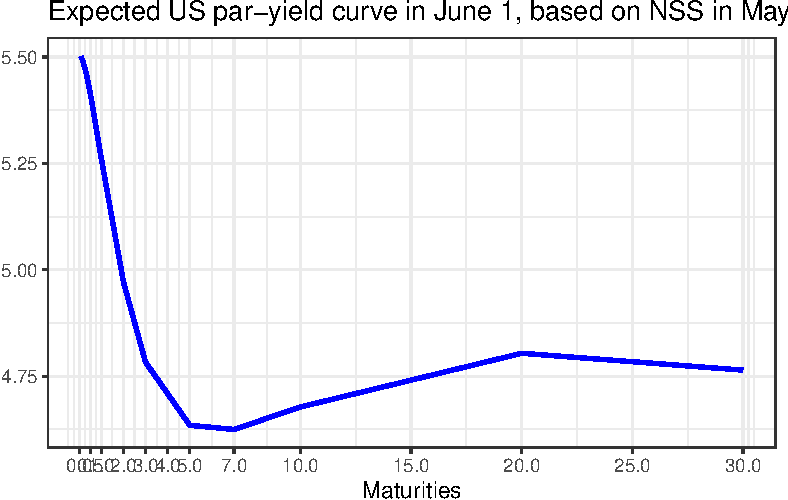
\includegraphics{이자율기간구조_hw2_files/figure-pdf/unnamed-chunk-13-1.pdf}

\section*{Problem 5}\label{problem-5}
\addcontentsline{toc}{section}{Problem 5}

\markright{Problem 5}

hw2.xlsx 에는 2011-10-28 부터 2016-10-28 까지의 스왑 데이터가 결측치가
있는 날들은 제외하고 들어 있다. 이를 이용하여 일별 금리변화를 주도하는
세 가지 주성분을 구하여 리포트하시오.

\subsection*{Answer}\label{answer-9}
\addcontentsline{toc}{subsection}{Answer}

먼저, 예제파일을 읽어와 일별/만기별 스왑금리의 차이를 bp단위로
계산하겠습니다.

\begin{Shaded}
\begin{Highlighting}[]
\NormalTok{pca }\OtherTok{\textless{}{-}} \FunctionTok{read\_csv}\NormalTok{(}\StringTok{"investment\_hw/term\_hw2.csv"}\NormalTok{) }\SpecialCharTok{\%\textgreater{}\%} 
  \FunctionTok{pivot\_longer}\NormalTok{(}\AttributeTok{cols=}\FunctionTok{contains}\NormalTok{(}\StringTok{"DSWP"}\NormalTok{),}\AttributeTok{names\_to =} \StringTok{"maturity"}\NormalTok{, }\AttributeTok{values\_to =} \StringTok{"rate"}\NormalTok{) }\SpecialCharTok{\%\textgreater{}\%} 
  \FunctionTok{arrange}\NormalTok{(maturity,observation\_date) }\SpecialCharTok{\%\textgreater{}\%} 
  \FunctionTok{mutate}\NormalTok{(}\AttributeTok{changes=}\NormalTok{(rate}\SpecialCharTok{{-}}\FunctionTok{lag}\NormalTok{(rate))}\SpecialCharTok{*}\DecValTok{100}\NormalTok{) }\SpecialCharTok{\%\textgreater{}\%} 
  \FunctionTok{filter}\NormalTok{(maturity}\SpecialCharTok{==}\FunctionTok{lag}\NormalTok{(maturity)) }\SpecialCharTok{\%\textgreater{}\%} 
  \FunctionTok{mutate}\NormalTok{(}\AttributeTok{date=}\NormalTok{observation\_date,}
         \AttributeTok{maturity=}\FunctionTok{substr}\NormalTok{(maturity,}\DecValTok{5}\NormalTok{,}\FunctionTok{nchar}\NormalTok{(maturity)) }\SpecialCharTok{\%\textgreater{}\%} \FunctionTok{as.integer}\NormalTok{()) }\SpecialCharTok{\%\textgreater{}\%} 
  \FunctionTok{select}\NormalTok{(date,maturity,changes)}
\end{Highlighting}
\end{Shaded}

다음으로, 각 만기별 covariance matrix를 산출하면 아래와 같습니다.

\begin{Shaded}
\begin{Highlighting}[]
\NormalTok{cov\_matrix }\OtherTok{\textless{}{-}}\NormalTok{ pca }\SpecialCharTok{\%\textgreater{}\%} 
  \FunctionTok{pivot\_wider}\NormalTok{(}\AttributeTok{names\_from =} \StringTok{"maturity"}\NormalTok{, }\AttributeTok{values\_from =} \StringTok{"changes"}\NormalTok{)}
\NormalTok{cov\_matrix }\OtherTok{\textless{}{-}}\NormalTok{ cov\_matrix[,}\DecValTok{2}\SpecialCharTok{:}\FunctionTok{ncol}\NormalTok{(cov\_matrix)] }\SpecialCharTok{\%\textgreater{}\%} 
  \FunctionTok{select}\NormalTok{(}\StringTok{\textasciigrave{}}\AttributeTok{1}\StringTok{\textasciigrave{}}\NormalTok{,}\StringTok{\textasciigrave{}}\AttributeTok{2}\StringTok{\textasciigrave{}}\NormalTok{,}\StringTok{\textasciigrave{}}\AttributeTok{3}\StringTok{\textasciigrave{}}\NormalTok{,}\StringTok{\textasciigrave{}}\AttributeTok{4}\StringTok{\textasciigrave{}}\NormalTok{,}\StringTok{\textasciigrave{}}\AttributeTok{5}\StringTok{\textasciigrave{}}\NormalTok{,}\StringTok{\textasciigrave{}}\AttributeTok{7}\StringTok{\textasciigrave{}}\NormalTok{,}\StringTok{\textasciigrave{}}\AttributeTok{10}\StringTok{\textasciigrave{}}\NormalTok{,}\StringTok{\textasciigrave{}}\AttributeTok{30}\StringTok{\textasciigrave{}}\NormalTok{) }\SpecialCharTok{\%\textgreater{}\%} 
  \FunctionTok{cov}\NormalTok{()}
\NormalTok{cov\_matrix}
\end{Highlighting}
\end{Shaded}

\begin{verbatim}
          1        2         3         4         5         7        10
1  2.213323 3.054846  3.522954  3.695589  3.704325  3.430568  2.954751
2  3.054846 5.697003  7.042143  7.838627  8.177007  8.046440  7.337582
3  3.522954 7.042143  9.896073 11.304172 12.094984 12.313863 11.528464
4  3.695589 7.838627 11.304172 13.825330 14.949418 15.678205 15.021017
5  3.704325 8.177007 12.094984 14.949418 16.859309 17.864806 17.438665
7  3.430568 8.046440 12.313863 15.678205 17.864806 20.054159 20.056503
10 2.954751 7.337582 11.528464 15.021017 17.438665 20.056503 21.083989
30 2.097906 5.747695  9.366056 12.600163 15.006896 18.130390 19.854240
          30
1   2.097906
2   5.747695
3   9.366056
4  12.600163
5  15.006896
7  18.130390
10 19.854240
30 21.117480
\end{verbatim}

이제, 공분산행렬을 통해 eigenvalue와 eigenvector를 계산하겠습니다.

\begin{Shaded}
\begin{Highlighting}[]
\NormalTok{eigenstuff }\OtherTok{\textless{}{-}} \FunctionTok{eigen}\NormalTok{(cov\_matrix)}
\NormalTok{eigenstuff}
\end{Highlighting}
\end{Shaded}

\begin{verbatim}
eigen() decomposition
$values
[1] 97.7556083  9.9072058  1.7152969  0.5055678  0.2766216  0.2128816  0.1902696
[8]  0.1832123

$vectors
            [,1]        [,2]       [,3]        [,4]        [,5]        [,6]
[1,] -0.08566499 -0.28417368  0.5079515  0.59000453  0.44063641 -0.32531917
[2,] -0.19277666 -0.39767870  0.4590348  0.05125766 -0.39712195  0.61693318
[3,] -0.28762263 -0.39863035  0.1332283 -0.40841549 -0.31307253 -0.42429611
[4,] -0.35996508 -0.30873249 -0.1546417 -0.29835459  0.19392700 -0.30442253
[5,] -0.40648106 -0.19685756 -0.3122795 -0.04801149  0.46000357  0.44075264
[6,] -0.44890229  0.04588149 -0.3212347  0.29085506  0.01963346  0.06933697
[7,] -0.45265726  0.28606038 -0.1312437  0.43331839 -0.50253489 -0.19855324
[8,] -0.41419598  0.61982781  0.5212229 -0.34464771  0.21904691  0.04864903
            [,7]        [,8]
[1,] -0.06279146  0.04302287
[2,]  0.16365769 -0.16202567
[3,] -0.22186257  0.49653749
[4,]  0.32446983 -0.65316035
[5,] -0.53295108  0.07933235
[6,]  0.62948968  0.45512949
[7,] -0.36366915 -0.28993305
[8,]  0.04712063  0.03508783
\end{verbatim}

해당 \textbf{eigenvalue는 각 주성분의 설명력}을 나타냅니다. 각
eigenvalue의 전체 합에 대한 \textbf{비율은 전체 금리변화에서 해당
주성분이 설명하는 비율}을 나타냅니다.

\begin{Shaded}
\begin{Highlighting}[]
\NormalTok{eigenstuff}\SpecialCharTok{$}\NormalTok{ratio}\OtherTok{=}\NormalTok{eigenstuff}\SpecialCharTok{$}\NormalTok{values}\SpecialCharTok{/}\FunctionTok{sum}\NormalTok{(eigenstuff}\SpecialCharTok{$}\NormalTok{values)}
\NormalTok{eigenstuff}\SpecialCharTok{$}\NormalTok{ratio}
\end{Highlighting}
\end{Shaded}

\begin{verbatim}
[1] 0.882695739 0.089458278 0.015488474 0.004565084 0.002497787 0.001922239
[7] 0.001718062 0.001654337
\end{verbatim}

이에 따르면, \textbf{첫번째 주성분이 약 88.3\%, 두번째 주성분이 8.9\%,
세번째 주성분이 1.5\%를 설명}하고 있습니다. 이는 \textbf{3가지의
주성분만으로 전체 swap rate curve 변화의 약 98.8\%를 설명}할 수 있다는
의미입니다.

여기에서, \textbf{첫번째 주성분}은 \textbf{전체적인 금리수준의
변화(level change effect)}라고 할 수 있고 \textbf{두번째 주성분}은
\textbf{금리곡선의 기울기 변화(slope change effect)}, \textbf{세번째
주성분}은 \textbf{금리곡선의 볼록성 변화(convecture change effect)}라고
할 수 있습니다.

세가지 주성분의 eigenvector를 도식화하면 아래와 같습니다.

\begin{Shaded}
\begin{Highlighting}[]
\NormalTok{plot\_pca }\OtherTok{\textless{}{-}} \FunctionTok{tibble}\NormalTok{(}\AttributeTok{maturity=}\FunctionTok{c}\NormalTok{(}\DecValTok{1}\SpecialCharTok{:}\DecValTok{8}\NormalTok{),}
                   \AttributeTok{PC1=}\NormalTok{eigenstuff}\SpecialCharTok{$}\NormalTok{vectors[,}\DecValTok{1}\NormalTok{],}
                   \AttributeTok{PC2=}\NormalTok{eigenstuff}\SpecialCharTok{$}\NormalTok{vectors[,}\DecValTok{2}\NormalTok{],}
                   \AttributeTok{PC3=}\NormalTok{eigenstuff}\SpecialCharTok{$}\NormalTok{vectors[,}\DecValTok{3}\NormalTok{]) }\SpecialCharTok{\%\textgreater{}\%} 
  \FunctionTok{pivot\_longer}\NormalTok{(}\AttributeTok{cols=}\FunctionTok{contains}\NormalTok{(}\StringTok{"PC"}\NormalTok{),}\AttributeTok{names\_to =} \StringTok{"components"}\NormalTok{, }\AttributeTok{values\_to =} \StringTok{"values"}\NormalTok{) }\SpecialCharTok{\%\textgreater{}\%} 
  \FunctionTok{ggplot}\NormalTok{(.,}\FunctionTok{aes}\NormalTok{(}\AttributeTok{x=}\NormalTok{maturity,}\AttributeTok{y=}\NormalTok{values,}\AttributeTok{colour=}\NormalTok{components))}\SpecialCharTok{+}
  \FunctionTok{geom\_line}\NormalTok{(}\AttributeTok{size=}\DecValTok{1}\NormalTok{)}\SpecialCharTok{+}
  \FunctionTok{theme\_bw}\NormalTok{()}
\NormalTok{plot\_pca}
\end{Highlighting}
\end{Shaded}

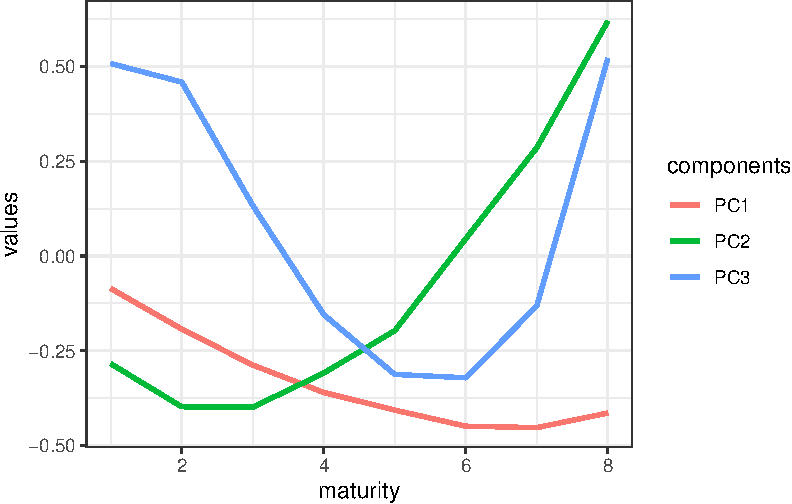
\includegraphics{이자율기간구조_hw2_files/figure-pdf/unnamed-chunk-18-1.pdf}

\part{투자분석('24봄)}

\chapter*{투자분석 과제1}\label{uxd22cuxc790uxbd84uxc11d-uxacfcuxc81c1}
\addcontentsline{toc}{chapter}{투자분석 과제1}

\markboth{투자분석 과제1}{투자분석 과제1}

\section*{\texorpdfstring{\textbf{\emph{Question}}}{Question}}\label{question}
\addcontentsline{toc}{section}{\textbf{\emph{Question}}}

\markright{\textbf{\emph{Question}}}

You are a stock analyst and want to evaluate stocks. You may select any
3 stocks and get information from data source you prefer. You need a
risk-free rate and market risk premium for this assignment. Choose
appropriate risk-free rate such as 3-month T-bill rate or 1-month LIBOR
and risk premium for the market portfolio. Use the constant growth
dividend discount model. You may use any computer tool but do not hand
in the data or the program code.

\begin{enumerate}
\def\labelenumi{\alph{enumi})}
\tightlist
\item
  What are the names of stocks you choose?
\item
  Specify risk-free rate, risk premium and the data source.
\item
  What are the required rates of return? Use the CAPM. You need to
  specify firm's beta and the expected rate of return of the market
  index portfolio.
\item
  Calculate present value of growth opportunity (PVGO) for each stock.
\item
  Find the intrinsic value (𝑉0) and 1-year value (𝑉1) for each stock.
\item
  Find the expected rate of return for each stock, i.e., (𝑉1 − 𝑃0)/𝑃0
  where 𝑃0 is the current market price.
\item
  Based on the calculation above, which stock do you buy or sell?
  Explain briefly
\end{enumerate}

\section*{문제풀이}\label{uxbb38uxc81cuxd480uxc774}
\addcontentsline{toc}{section}{문제풀이}

\markright{문제풀이}

\subsection*{(a) 주식 선정}\label{a-uxc8fcuxc2dd-uxc120uxc815}
\addcontentsline{toc}{subsection}{(a) 주식 선정}

저는 \textbf{\emph{CME group(CME), ICE(ICE), Nasdaq(NDAQ)}} 세가지
종목을 선정하였습니다.

선정 배경으로는,

\begin{enumerate}
\def\labelenumi{(\arabic{enumi})}
\tightlist
\item
  제가 거래소 산업에 관심이 많고,
\item
  세 주식 모두 미국에 상장되어있는 대표적인 글로벌 거래소이며,
\item
  동일한 거래소 산업이고 S\&P500지수의 구성종목이라 동일 선상에서
  비교하기 적합할 것으로 보이기 때문입니다.
\end{enumerate}

관련 자료는 \href{https://finance.yahoo.com/}{Yahoo Finance}를
참조하였습니다.

\subsection*{(b) 무위험이자율 및
리스크프리미엄}\label{b-uxbb34uxc704uxd5d8uxc774uxc790uxc728-uxbc0f-uxb9acuxc2a4uxd06cuxd504uxb9acuxbbf8uxc5c4}
\addcontentsline{toc}{subsection}{(b) 무위험이자율 및 리스크프리미엄}

risk-free rate는 최근 미국에서 대체지표금리로 선정한 SOFR기반의 금리를
누적하여 3개월 금리로 환산한 3-month SOFR Average를 risk-free rate로
선정하였습니다.

\href{https://www.newyorkfed.org/markets/reference-rates/sofr-averages-and-index}{NewYork
Fed : SOFR Average}

각 주식과 시장(S\&P500)의 리스크프리미엄은 과거
3년간('21\textasciitilde'23)의 연평균수익률 및 무위험이자율을 이용하여
산출할 예정입니다.

각 데이터를 취합하여 정리한 결과 및 무위험이자율, 리스크프리미엄의
산출은 아래와 같습니다.

\begin{Shaded}
\begin{Highlighting}[]
\CommentTok{\# import data\&library}
\FunctionTok{rm}\NormalTok{(}\AttributeTok{list =} \FunctionTok{ls}\NormalTok{())}
\FunctionTok{library}\NormalTok{(tidyverse)}
\NormalTok{nasdaq }\OtherTok{\textless{}{-}} \FunctionTok{read\_csv}\NormalTok{(}\StringTok{"investment\_hw/투자분석\_NDAQ.csv"}\NormalTok{)}
\NormalTok{cme }\OtherTok{\textless{}{-}} \FunctionTok{read\_csv}\NormalTok{(}\StringTok{"investment\_hw/투자분석\_CME.csv"}\NormalTok{)}
\NormalTok{ice }\OtherTok{\textless{}{-}} \FunctionTok{read\_csv}\NormalTok{(}\StringTok{"investment\_hw/투자분석\_ICE.csv"}\NormalTok{)}
\NormalTok{rf }\OtherTok{\textless{}{-}} \FunctionTok{read\_csv}\NormalTok{(}\StringTok{"investment\_hw/투자분석\_sofrai.csv"}\NormalTok{)}
\NormalTok{market }\OtherTok{\textless{}{-}} \FunctionTok{read\_csv}\NormalTok{(}\StringTok{"investment\_hw/투자분석\_snp500.csv"}\NormalTok{)}

\CommentTok{\# tidy data}
\NormalTok{rf2 }\OtherTok{\textless{}{-}}\NormalTok{ rf }\SpecialCharTok{\%\textgreater{}\%} 
  \FunctionTok{filter}\NormalTok{(}\StringTok{\textasciigrave{}}\AttributeTok{90{-}Day Average SOFR}\StringTok{\textasciigrave{}} \SpecialCharTok{\%\textgreater{}\%} \FunctionTok{is.na}\NormalTok{()}\SpecialCharTok{==}\ConstantTok{FALSE}\NormalTok{) }\SpecialCharTok{\%\textgreater{}\%} 
  \FunctionTok{mutate}\NormalTok{(}\AttributeTok{date=}\FunctionTok{paste0}\NormalTok{(}\FunctionTok{substr}\NormalTok{(}\StringTok{\textasciigrave{}}\AttributeTok{Effective Date}\StringTok{\textasciigrave{}}\NormalTok{,}\DecValTok{7}\NormalTok{,}\DecValTok{10}\NormalTok{),}
                     \FunctionTok{substr}\NormalTok{(}\StringTok{\textasciigrave{}}\AttributeTok{Effective Date}\StringTok{\textasciigrave{}}\NormalTok{,}\DecValTok{1}\NormalTok{,}\DecValTok{2}\NormalTok{),}
                     \FunctionTok{substr}\NormalTok{(}\StringTok{\textasciigrave{}}\AttributeTok{Effective Date}\StringTok{\textasciigrave{}}\NormalTok{,}\DecValTok{4}\NormalTok{,}\DecValTok{5}\NormalTok{)) }\SpecialCharTok{\%\textgreater{}\%} \FunctionTok{as.integer}\NormalTok{(),}
         \AttributeTok{year=}\FunctionTok{substr}\NormalTok{(}\StringTok{\textasciigrave{}}\AttributeTok{Effective Date}\StringTok{\textasciigrave{}}\NormalTok{,}\DecValTok{7}\NormalTok{,}\DecValTok{10}\NormalTok{),}
         \AttributeTok{month=}\FunctionTok{substr}\NormalTok{(}\StringTok{\textasciigrave{}}\AttributeTok{Effective Date}\StringTok{\textasciigrave{}}\NormalTok{,}\DecValTok{1}\NormalTok{,}\DecValTok{2}\NormalTok{),}
         \AttributeTok{group=}\StringTok{"rfr"}\NormalTok{,}
         \AttributeTok{price=}\StringTok{\textasciigrave{}}\AttributeTok{90{-}Day Average SOFR}\StringTok{\textasciigrave{}}\NormalTok{) }\SpecialCharTok{\%\textgreater{}\%} 
  \FunctionTok{select}\NormalTok{(year,month,date,group,price)}

\CommentTok{\# Data Pre{-}processing}
\NormalTok{tidydata }\OtherTok{\textless{}{-}} \FunctionTok{tibble}\NormalTok{()}
\NormalTok{tidydata }\OtherTok{\textless{}{-}}\NormalTok{ nasdaq }\SpecialCharTok{\%\textgreater{}\%} 
  \FunctionTok{mutate}\NormalTok{(}\AttributeTok{group=}\StringTok{"nasdaq"}\NormalTok{) }\SpecialCharTok{\%\textgreater{}\%} 
  \FunctionTok{union\_all}\NormalTok{(cme }\SpecialCharTok{\%\textgreater{}\%} \FunctionTok{mutate}\NormalTok{(}\AttributeTok{group=}\StringTok{"cme"}\NormalTok{)) }\SpecialCharTok{\%\textgreater{}\%} 
  \FunctionTok{union\_all}\NormalTok{(ice }\SpecialCharTok{\%\textgreater{}\%} \FunctionTok{mutate}\NormalTok{(}\AttributeTok{group=}\StringTok{"ice"}\NormalTok{)) }\SpecialCharTok{\%\textgreater{}\%} 
  \FunctionTok{union\_all}\NormalTok{(market }\SpecialCharTok{\%\textgreater{}\%} \FunctionTok{mutate}\NormalTok{(}\AttributeTok{group=}\StringTok{"market"}\NormalTok{)) }\SpecialCharTok{\%\textgreater{}\%} 
  \FunctionTok{mutate}\NormalTok{(}\AttributeTok{date=}\FunctionTok{paste0}\NormalTok{(}\FunctionTok{substr}\NormalTok{(Date,}\DecValTok{1}\NormalTok{,}\DecValTok{4}\NormalTok{),}
                     \FunctionTok{substr}\NormalTok{(Date,}\DecValTok{6}\NormalTok{,}\DecValTok{7}\NormalTok{),}
                     \FunctionTok{substr}\NormalTok{(Date,}\DecValTok{9}\NormalTok{,}\DecValTok{10}\NormalTok{)) }\SpecialCharTok{\%\textgreater{}\%} \FunctionTok{as.integer}\NormalTok{(),}
         \AttributeTok{year=}\FunctionTok{substr}\NormalTok{(Date,}\DecValTok{1}\NormalTok{,}\DecValTok{4}\NormalTok{),}
         \AttributeTok{month=}\FunctionTok{substr}\NormalTok{(Date,}\DecValTok{6}\NormalTok{,}\DecValTok{7}\NormalTok{),}
         \AttributeTok{price=}\StringTok{\textasciigrave{}}\AttributeTok{Adj Close}\StringTok{\textasciigrave{}}\NormalTok{) }\SpecialCharTok{\%\textgreater{}\%} 
  \FunctionTok{select}\NormalTok{(year,month,date,group,price) }\SpecialCharTok{\%\textgreater{}\%} 
  \FunctionTok{union\_all}\NormalTok{(rf2) }\SpecialCharTok{\%\textgreater{}\%} 
  \FunctionTok{arrange}\NormalTok{(date,group)}

\CommentTok{\# Use daily adj. closing price, if rfr is NA then use yesterday rfr.}
\NormalTok{tidydata\_wide }\OtherTok{\textless{}{-}}\NormalTok{ tidydata }\SpecialCharTok{\%\textgreater{}\%} 
  \FunctionTok{pivot\_wider}\NormalTok{(}\AttributeTok{names\_from =} \StringTok{"group"}\NormalTok{, }\AttributeTok{values\_from =} \StringTok{"price"}\NormalTok{) }\SpecialCharTok{\%\textgreater{}\%} 
  \FunctionTok{filter}\NormalTok{(nasdaq }\SpecialCharTok{\%\textgreater{}\%} \FunctionTok{is.na}\NormalTok{()}\SpecialCharTok{==}\ConstantTok{FALSE}\NormalTok{,}
\NormalTok{         cme }\SpecialCharTok{\%\textgreater{}\%} \FunctionTok{is.na}\NormalTok{()}\SpecialCharTok{==}\ConstantTok{FALSE}\NormalTok{,}
\NormalTok{         ice }\SpecialCharTok{\%\textgreater{}\%} \FunctionTok{is.na}\NormalTok{()}\SpecialCharTok{==}\ConstantTok{FALSE}\NormalTok{,}
\NormalTok{         market }\SpecialCharTok{\%\textgreater{}\%} \FunctionTok{is.na}\NormalTok{()}\SpecialCharTok{==}\ConstantTok{FALSE}\NormalTok{) }\SpecialCharTok{\%\textgreater{}\%} 
  \FunctionTok{mutate}\NormalTok{(}\AttributeTok{rfr=}\FunctionTok{if\_else}\NormalTok{(rfr }\SpecialCharTok{\%\textgreater{}\%} \FunctionTok{is.na}\NormalTok{(),}\FunctionTok{lag}\NormalTok{(rfr)}\SpecialCharTok{/}\DecValTok{100}\NormalTok{,rfr}\SpecialCharTok{/}\DecValTok{100}\NormalTok{)) }\SpecialCharTok{\%\textgreater{}\%} 
  \FunctionTok{mutate}\NormalTok{(}\AttributeTok{cme\_yield=}\FunctionTok{log}\NormalTok{(cme)}\SpecialCharTok{{-}}\FunctionTok{log}\NormalTok{(}\FunctionTok{lag}\NormalTok{(cme)),}
         \AttributeTok{ice\_yield=}\FunctionTok{log}\NormalTok{(ice)}\SpecialCharTok{{-}}\FunctionTok{log}\NormalTok{(}\FunctionTok{lag}\NormalTok{(ice)),}
         \AttributeTok{nasdaq\_yield=}\FunctionTok{log}\NormalTok{(nasdaq)}\SpecialCharTok{{-}}\FunctionTok{log}\NormalTok{(}\FunctionTok{lag}\NormalTok{(nasdaq)),}
         \AttributeTok{market\_yield=}\FunctionTok{log}\NormalTok{(market)}\SpecialCharTok{{-}}\FunctionTok{log}\NormalTok{(}\FunctionTok{lag}\NormalTok{(market))) }\SpecialCharTok{\%\textgreater{}\%} 
  \FunctionTok{filter}\NormalTok{(cme\_yield }\SpecialCharTok{\%\textgreater{}\%} \FunctionTok{is.na}\NormalTok{()}\SpecialCharTok{==}\ConstantTok{FALSE}\NormalTok{)}
\end{Highlighting}
\end{Shaded}

\begin{Shaded}
\begin{Highlighting}[]
\NormalTok{rf3 }\OtherTok{\textless{}{-}}\NormalTok{ tidydata\_wide }\SpecialCharTok{\%\textgreater{}\%} 
  \FunctionTok{filter}\NormalTok{(year}\SpecialCharTok{!=}\DecValTok{2020}\SpecialCharTok{\&}\NormalTok{year}\SpecialCharTok{!=}\DecValTok{2024}\NormalTok{,}\FunctionTok{as.integer}\NormalTok{(month)}\SpecialCharTok{\%\%}\DecValTok{3}\SpecialCharTok{==}\DecValTok{0}\NormalTok{) }\SpecialCharTok{\%\textgreater{}\%} 
  \FunctionTok{arrange}\NormalTok{(date }\SpecialCharTok{\%\textgreater{}\%} \FunctionTok{desc}\NormalTok{()) }\SpecialCharTok{\%\textgreater{}\%} 
  \FunctionTok{group\_by}\NormalTok{(year,month) }\SpecialCharTok{\%\textgreater{}\%} 
  \FunctionTok{slice}\NormalTok{(}\DecValTok{1}\NormalTok{) }\SpecialCharTok{\%\textgreater{}\%} 
  \FunctionTok{ungroup}\NormalTok{() }\SpecialCharTok{\%\textgreater{}\%} 
  \FunctionTok{summarise}\NormalTok{(}\AttributeTok{rfr\_3year=}\FunctionTok{mean}\NormalTok{(rfr))}

\NormalTok{tidydata\_wide }\SpecialCharTok{\%\textgreater{}\%} \FunctionTok{filter}\NormalTok{(date}\SpecialCharTok{==}\DecValTok{20231229}\NormalTok{) }\SpecialCharTok{\%\textgreater{}\%} \FunctionTok{select}\NormalTok{(rfr) }\SpecialCharTok{\%\textgreater{}\%} \FunctionTok{bind\_cols}\NormalTok{(rf3)}
\end{Highlighting}
\end{Shaded}

\begin{verbatim}
# A tibble: 1 x 2
     rfr rfr_3year
   <dbl>     <dbl>
1 0.0536    0.0223
\end{verbatim}

\begin{Shaded}
\begin{Highlighting}[]
\NormalTok{tidydata\_wide }\SpecialCharTok{\%\textgreater{}\%} 
  \FunctionTok{filter}\NormalTok{(year}\SpecialCharTok{!=}\DecValTok{2020}\SpecialCharTok{\&}\NormalTok{year}\SpecialCharTok{!=}\DecValTok{2024}\NormalTok{) }\SpecialCharTok{\%\textgreater{}\%} 
  \FunctionTok{summarise}\NormalTok{(}\AttributeTok{cme\_premium=}\FunctionTok{sum}\NormalTok{(cme\_yield)}\SpecialCharTok{/}\DecValTok{3}\SpecialCharTok{{-}}\NormalTok{rf3}\SpecialCharTok{$}\NormalTok{rfr\_3year,}
            \AttributeTok{ice\_premium=}\FunctionTok{sum}\NormalTok{(ice\_yield)}\SpecialCharTok{/}\DecValTok{3}\SpecialCharTok{{-}}\NormalTok{rf3}\SpecialCharTok{$}\NormalTok{rfr\_3year,}
            \AttributeTok{nasdaq\_premium=}\FunctionTok{sum}\NormalTok{(nasdaq\_yield)}\SpecialCharTok{/}\DecValTok{3}\SpecialCharTok{{-}}\NormalTok{rf3}\SpecialCharTok{$}\NormalTok{rfr\_3year,}
            \AttributeTok{market\_premium=}\FunctionTok{sum}\NormalTok{(market\_yield)}\SpecialCharTok{/}\DecValTok{3}\SpecialCharTok{{-}}\NormalTok{rf3}\SpecialCharTok{$}\NormalTok{rfr\_3year)}
\end{Highlighting}
\end{Shaded}

\begin{verbatim}
# A tibble: 1 x 4
  cme_premium ice_premium nasdaq_premium market_premium
        <dbl>       <dbl>          <dbl>          <dbl>
1      0.0679      0.0272         0.0826         0.0573
\end{verbatim}

무위험이자율은 기간말 기준 5.36\%, 과거 3개년 동안 무위험이자율에 투자한
연평균수익률은 약 2.23\%, 과거 3개년 동안 실현된 각 주식과 시장의 연환산
리스크프리미엄은 아래 표와 같습니다.

\begin{longtable}[]{@{}ccccc@{}}
\toprule\noalign{}
구 분 & S\&P500 & CME & ICE & NASDAQ \\
\midrule\noalign{}
\endhead
\bottomrule\noalign{}
\endlastfoot
연수익률 & 7.96\% & 9.03\%\% & 4.95\% & 10.49\% \\
프리미엄 & 5.74\% & 6.81\%\% & 2.73\% & 8.27\% \\
\end{longtable}

\begin{tcolorbox}[enhanced jigsaw, toprule=.15mm, colframe=quarto-callout-warning-color-frame, opacitybacktitle=0.6, bottomtitle=1mm, left=2mm, breakable, coltitle=black, title=\textcolor{quarto-callout-warning-color}{\faExclamationTriangle}\hspace{0.5em}{Excess return vs.~Risk premium}, colbacktitle=quarto-callout-warning-color!10!white, opacityback=0, bottomrule=.15mm, toptitle=1mm, leftrule=.75mm, titlerule=0mm, colback=white, arc=.35mm, rightrule=.15mm]

초과수익률은 과거의 값을 바탕으로 산출되며, 리스크프리미엄은
기대수익률을 기반으로 산출.

위의 풀이는 초과수익률을 산출하였으므로 오답이며, 리스크프리미엄은 CAPM
등의 기대수익률을 가지고와서 산출해야 함. \[Excess\;return = r-r_f\]
\[Risk\;premium = E[r]-r_f\]

\end{tcolorbox}

\subsection*{(c) CAPM}\label{c-capm}
\addcontentsline{toc}{subsection}{(c) CAPM}

각 종목의 베타를 산출하기 위해 필요한 파라미터는 아래와 같습니다.

\begin{itemize}
\tightlist
\item
  무위험이자율, \(R_f\) : 기간말('23.12월말)의 3-month SOFR average
\item
  시장수익률, \(R_m\) : S\&P500지수의 수익률
\item
  개별수익률, \(R_{stock}\) : 개별 주식의 수익률
\end{itemize}

수익률은 일간/월간 두가지를 사용하여 비교할 예정이며, 회귀분석에 사용한
값은 아래와 같습니다.

\begin{itemize}
\tightlist
\item
  기간 : (일별) 2023년 250거래일, (월간) 2021년\textasciitilde2023년
  36개월
\item
  산출방법 : (일별) 전일 종가 대비 당일 종가의 로그수익률, (월별) 이전달
  말 종가 대비 이번달 말 종가의 로그수익률
\end{itemize}

마지막으로, 베타를 이용하여 기대수익률을 산출할 때 이용한 \(R_m\)은
다음과 같습니다.

\begin{itemize}
\tightlist
\item
  (일별) 250일간 S\&P500지수 일평균수익률의 연환산(=연수익률)
\item
  (월별) 36개월간 S\&P500지수 월평균수익률의 연환산(=3개년수익률/3)
\end{itemize}

\begin{tcolorbox}[enhanced jigsaw, toprule=.15mm, colframe=quarto-callout-warning-color-frame, opacitybacktitle=0.6, bottomtitle=1mm, left=2mm, breakable, coltitle=black, title=\textcolor{quarto-callout-warning-color}{\faExclamationTriangle}\hspace{0.5em}{Warning}, colbacktitle=quarto-callout-warning-color!10!white, opacityback=0, bottomrule=.15mm, toptitle=1mm, leftrule=.75mm, titlerule=0mm, colback=white, arc=.35mm, rightrule=.15mm]

로그수익률(연속복리수익률)을 사용하였으므로 보유기간수익률로 표현할 때
단순 덧셈만으로 환산할 수 있습니다.

또한, 기간 중 배당 및 CA로 인한 차이는 수정주가(Adj. close price)를
사용해서 보정하였습니다.

\end{tcolorbox}

이에 따라, R코드로 산출한 개별종목별 \textbf{베타 / 기대수익률 /
산출기간동안 실현수익률}은 아래와 같습니다.

\begin{Shaded}
\begin{Highlighting}[]
\CommentTok{\# calcuate beta, required return}

\CommentTok{\# daily beta in \textquotesingle{}23}
\NormalTok{dailybeta }\OtherTok{\textless{}{-}}\NormalTok{ tidydata\_wide }\SpecialCharTok{\%\textgreater{}\%} 
  \FunctionTok{filter}\NormalTok{(year}\SpecialCharTok{==}\StringTok{"2023"}\NormalTok{) }\SpecialCharTok{\%\textgreater{}\%} 
  \FunctionTok{summarise}\NormalTok{(}\AttributeTok{beta\_cme=}\FunctionTok{cov}\NormalTok{(market\_yield,cme\_yield)}\SpecialCharTok{/}\FunctionTok{var}\NormalTok{(market\_yield),}
            \AttributeTok{beta\_ice=}\FunctionTok{cov}\NormalTok{(market\_yield,ice\_yield)}\SpecialCharTok{/}\FunctionTok{var}\NormalTok{(market\_yield),}
            \AttributeTok{beta\_nasdaq=}\FunctionTok{cov}\NormalTok{(market\_yield,nasdaq\_yield)}\SpecialCharTok{/}\FunctionTok{var}\NormalTok{(market\_yield),}
            \AttributeTok{market\_avg\_yield=}\FunctionTok{sum}\NormalTok{(market\_yield),}
            \AttributeTok{cme\_avg\_yield=}\FunctionTok{sum}\NormalTok{(cme\_yield),}
            \AttributeTok{ice\_avg\_yield=}\FunctionTok{sum}\NormalTok{(ice\_yield),}
            \AttributeTok{nasdaq\_avg\_yield=}\FunctionTok{sum}\NormalTok{(nasdaq\_yield)) }\SpecialCharTok{\%\textgreater{}\%} 
  \FunctionTok{mutate}\NormalTok{(}\AttributeTok{group=}\StringTok{"daily"}\NormalTok{)}

\CommentTok{\# monthly beta}
\NormalTok{monthlybeta }\OtherTok{\textless{}{-}}\NormalTok{ tidydata\_wide }\SpecialCharTok{\%\textgreater{}\%} 
  \FunctionTok{arrange}\NormalTok{(year,month,date }\SpecialCharTok{\%\textgreater{}\%}\NormalTok{ desc) }\SpecialCharTok{\%\textgreater{}\%} 
  \FunctionTok{group\_by}\NormalTok{(year,month) }\SpecialCharTok{\%\textgreater{}\%} 
  \FunctionTok{slice}\NormalTok{(}\DecValTok{1}\NormalTok{) }\SpecialCharTok{\%\textgreater{}\%} 
  \FunctionTok{ungroup}\NormalTok{() }\SpecialCharTok{\%\textgreater{}\%} 
  \FunctionTok{mutate}\NormalTok{(}\AttributeTok{cme\_yield=}\FunctionTok{log}\NormalTok{(cme)}\SpecialCharTok{{-}}\FunctionTok{log}\NormalTok{(}\FunctionTok{lag}\NormalTok{(cme)),}
         \AttributeTok{ice\_yield=}\FunctionTok{log}\NormalTok{(ice)}\SpecialCharTok{{-}}\FunctionTok{log}\NormalTok{(}\FunctionTok{lag}\NormalTok{(ice)),}
         \AttributeTok{nasdaq\_yield=}\FunctionTok{log}\NormalTok{(nasdaq)}\SpecialCharTok{{-}}\FunctionTok{log}\NormalTok{(}\FunctionTok{lag}\NormalTok{(nasdaq)),}
         \AttributeTok{market\_yield=}\FunctionTok{log}\NormalTok{(market)}\SpecialCharTok{{-}}\FunctionTok{log}\NormalTok{(}\FunctionTok{lag}\NormalTok{(market))) }\SpecialCharTok{\%\textgreater{}\%} 
  \FunctionTok{filter}\NormalTok{(cme\_yield }\SpecialCharTok{\%\textgreater{}\%} \FunctionTok{is.na}\NormalTok{()}\SpecialCharTok{==}\ConstantTok{FALSE}\NormalTok{) }\SpecialCharTok{\%\textgreater{}\%} 
  \FunctionTok{filter}\NormalTok{(year}\SpecialCharTok{!=}\StringTok{"2024"}\NormalTok{,year}\SpecialCharTok{!=}\StringTok{"2020"}\NormalTok{) }\SpecialCharTok{\%\textgreater{}\%} 
  \FunctionTok{summarise}\NormalTok{(}\AttributeTok{beta\_cme=}\FunctionTok{cov}\NormalTok{(market\_yield,cme\_yield)}\SpecialCharTok{/}\FunctionTok{var}\NormalTok{(market\_yield),}
            \AttributeTok{beta\_ice=}\FunctionTok{cov}\NormalTok{(market\_yield,ice\_yield)}\SpecialCharTok{/}\FunctionTok{var}\NormalTok{(market\_yield),}
            \AttributeTok{beta\_nasdaq=}\FunctionTok{cov}\NormalTok{(market\_yield,nasdaq\_yield)}\SpecialCharTok{/}\FunctionTok{var}\NormalTok{(market\_yield),}
            \AttributeTok{market\_avg\_yield=}\FunctionTok{sum}\NormalTok{(market\_yield)}\SpecialCharTok{/}\DecValTok{3}\NormalTok{,}
            \AttributeTok{cme\_avg\_yield=}\FunctionTok{sum}\NormalTok{(cme\_yield)}\SpecialCharTok{/}\DecValTok{3}\NormalTok{,}
            \AttributeTok{ice\_avg\_yield=}\FunctionTok{sum}\NormalTok{(ice\_yield)}\SpecialCharTok{/}\DecValTok{3}\NormalTok{,}
            \AttributeTok{nasdaq\_avg\_yield=}\FunctionTok{sum}\NormalTok{(nasdaq\_yield)}\SpecialCharTok{/}\DecValTok{3}\NormalTok{) }\SpecialCharTok{\%\textgreater{}\%} 
  \FunctionTok{mutate}\NormalTok{(}\AttributeTok{group=}\StringTok{"monthly"}\NormalTok{)}

\NormalTok{beta }\OtherTok{\textless{}{-}} \FunctionTok{tibble}\NormalTok{()}
\NormalTok{beta }\OtherTok{\textless{}{-}}\NormalTok{ dailybeta }\SpecialCharTok{\%\textgreater{}\%} 
  \FunctionTok{union\_all}\NormalTok{(monthlybeta) }\SpecialCharTok{\%\textgreater{}\%} 
  \FunctionTok{mutate}\NormalTok{(tidydata\_wide }\SpecialCharTok{\%\textgreater{}\%} \FunctionTok{filter}\NormalTok{(date}\SpecialCharTok{==}\DecValTok{20231229}\NormalTok{) }\SpecialCharTok{\%\textgreater{}\%} \FunctionTok{select}\NormalTok{(rfr)) }\SpecialCharTok{\%\textgreater{}\%} 
  \FunctionTok{select}\NormalTok{(group,market\_avg\_yield,cme\_avg\_yield,ice\_avg\_yield,nasdaq\_avg\_yield,}
\NormalTok{         rfr,beta\_cme,beta\_ice,beta\_nasdaq)}

\NormalTok{capm }\OtherTok{\textless{}{-}} \FunctionTok{tibble}\NormalTok{()}
\NormalTok{capm }\OtherTok{\textless{}{-}}\NormalTok{ beta }\SpecialCharTok{\%\textgreater{}\%} 
  \FunctionTok{pivot\_longer}\NormalTok{(}\AttributeTok{cols =} \FunctionTok{c}\NormalTok{(}\StringTok{"beta\_cme"}\NormalTok{,}\StringTok{"beta\_ice"}\NormalTok{,}\StringTok{"beta\_nasdaq"}\NormalTok{),}
               \AttributeTok{names\_to =} \StringTok{"stock"}\NormalTok{, }\AttributeTok{values\_to =} \StringTok{"beta"}\NormalTok{) }\SpecialCharTok{\%\textgreater{}\%} 
  \FunctionTok{mutate}\NormalTok{(}\AttributeTok{expected\_return=}\NormalTok{beta}\SpecialCharTok{*}\NormalTok{(market\_avg\_yield}\SpecialCharTok{{-}}\NormalTok{rfr)}\SpecialCharTok{+}\NormalTok{rfr) }\SpecialCharTok{\%\textgreater{}\%} 
  \FunctionTok{mutate}\NormalTok{(}\AttributeTok{stock=}\FunctionTok{substr}\NormalTok{(stock,}\DecValTok{6}\NormalTok{,}\FunctionTok{nchar}\NormalTok{(stock))) }\SpecialCharTok{\%\textgreater{}\%} 
  \FunctionTok{mutate}\NormalTok{(}\AttributeTok{realized\_return=}\FunctionTok{if\_else}\NormalTok{(stock}\SpecialCharTok{==}\StringTok{"cme"}\NormalTok{,cme\_avg\_yield,}
                                \FunctionTok{if\_else}\NormalTok{(stock}\SpecialCharTok{==}\StringTok{"ice"}\NormalTok{,ice\_avg\_yield,nasdaq\_avg\_yield))) }\SpecialCharTok{\%\textgreater{}\%} 
  \FunctionTok{select}\NormalTok{(group,stock,beta,expected\_return,realized\_return,market\_avg\_yield,rfr)}

\NormalTok{capm}
\end{Highlighting}
\end{Shaded}

\begin{verbatim}
# A tibble: 6 x 7
  group   stock   beta expected_return realized_return market_avg_yield    rfr
  <chr>   <chr>  <dbl>           <dbl>           <dbl>            <dbl>  <dbl>
1 daily   cme    0.315          0.105           0.272            0.217  0.0536
2 daily   ice    0.828          0.189           0.240            0.217  0.0536
3 daily   nasdaq 0.866          0.195          -0.0373           0.217  0.0536
4 monthly cme    0.353          0.0628          0.0903           0.0796 0.0536
5 monthly ice    1.12           0.0829          0.0495           0.0796 0.0536
6 monthly nasdaq 0.993          0.0795          0.105            0.0796 0.0536
\end{verbatim}

일별/월별로 구분한 각 주식의 베타와 기대수익률입니다.

보다 일반적이고 평탄화된 결과를 위해 월별 데이터를 중심으로
설명하겠습니다.

먼저 \textbf{각 주식의 베타는 CME:0.35, ICE:1.12, Nasdaq 0.99}입니다.
이는 거래소산업이 특성상 변동성이 크지 않고 경제상황에 민감하지 않아
베타가 시장포트폴리오와 유사한 1 수준에서 형성되는 것으로 보입니다.
특히, CME는 세계 최대의 파생상품거래소로서 규모가 매우 큰 고배당
우량주인 특징이 있어 변동성이 낮아 베타가 0.35로 낮게 형성된 것으로
추정됩니다.

\begin{tcolorbox}[enhanced jigsaw, toprule=.15mm, colframe=quarto-callout-color-frame, opacityback=0, bottomrule=.15mm, arc=.35mm, left=2mm, rightrule=.15mm, colback=white, breakable, leftrule=.75mm]

\vspace{-3mm}\textbf{베타 산출방법}\vspace{3mm}

베타는 \(R_{stock,t}=\alpha+\beta R_{m,t}+\epsilon\)의 선형회귀분석
결과로 산출되는 계수입니다.

즉,
\(\beta=\rho_{stock,m}\frac{\sigma_{stock}}{\sigma_m}=\frac{Cov_{stock,m}}{\sigma_m^2}\)로
산출할 수 있습니다.

\end{tcolorbox}

월별수익률을 산출한 과거 3년(2021\textasciitilde2023)간 평균월별수익률을
연율화하면 로그수익률 특성상 지난 3년간 연평균수익률과 같습니다. 즉,
시장포트폴리오의 기대수익률은 약 7.96\%라고 할 수 있으며, 무위험이자율은
2023.12월말 값인 5.36\%를 사용합니다.

이제, \(R_{stock}=\beta(R_m-R_f)+R_f\)를 통해 각 주식의 요구수익률을
산출할 수 있습니다.

\begin{longtable}[]{@{}cccc@{}}
\toprule\noalign{}
구 분 & CME & ICE & NASDAQ \\
\midrule\noalign{}
\endhead
\bottomrule\noalign{}
\endlastfoot
Beta & 0.35 & 1.12 & 0.99 \\
Required Return & 6.28\% & 8.29\% & 7.95\% \\
\end{longtable}

\subsection*{(d) PVGO}\label{d-pvgo}
\addcontentsline{toc}{subsection}{(d) PVGO}

먼저, 거래소산업은 성장주보다는 우량주 성향이 강하고, 배당성향이 다소
높고 정기적인 배당을 하는 경향이 있습니다.. 따라서
배당할인모형(Constant-growth DDM)을 사용할 예정입니다.

먼저, 기업의 내재가치에 배당할인모형을 적용한 PVGO의 산식은 아래와
같습니다. \[PVGO=V_0-\frac{E_1}{k}=\frac{D_1}{k-g}-\frac{E_1}{k}\]

여기서, 요구수익률 \(k\)는 (c)에서 CAPM으로 구한 요구수익률을 사용할
예정이며, \(D_1, E_1, g\)를 구하기 위해 직전주당배당(\(D_0\)), 직전
주당수익(\(E_0\)), 직전재투자성향(\(b_0=\frac{E_0-D_0}{E_0}\)), 직전
자기자본수익률 \(ROE_0\)를 이용하여 다음과 같이 산출하도록 하겠습니다.

\[g=b_0\times ROE_0=\frac{E_0-D_0}{E_0}\times ROE_0,\;\;D_1=D_0(1+g),\;\;E_1=E_0(1+g)\]

\[\Rrightarrow PVGO=\frac{D_0(1+g)}{k-g}-\frac{E_0(1+g)}{k}\]

\begin{tcolorbox}[enhanced jigsaw, toprule=.15mm, colframe=quarto-callout-note-color-frame, opacitybacktitle=0.6, bottomtitle=1mm, left=2mm, breakable, coltitle=black, title=\textcolor{quarto-callout-note-color}{\faInfo}\hspace{0.5em}{주당순이익 산출 : DDM}, colbacktitle=quarto-callout-note-color!10!white, opacityback=0, bottomrule=.15mm, toptitle=1mm, leftrule=.75mm, titlerule=0mm, colback=white, arc=.35mm, rightrule=.15mm]

다음 년도의 주당순이익 \(E_1\)은 올해의 순이익 \(E_0\)에 배당할인모형의
배당성장률 \(g\)를 반영하여 산출하였습니다.

\end{tcolorbox}

이제, 각 주식의 재무상태표를 참조하여 \(D_0\), \(E_0\), \(b_0\),
\(ROE_0\)를 산출하겠습니다. 다만, 직전사업연도(2023)는
시장벤치마크(S\&P500)의 수익률이 약 21\%로, 과거 평균치의 약 3배를
상회하고 있어 각 기업의 EPS, DPS 등이 평소 수치보다 고평가되었을
가능성이 있습니다. 이를 감안하여 \(D_0\), \(E_0\) 산출시에는 과거 3개년
당기순이익, 현금배당금의 산술평균을 사용할 것이며 \(ROE_0\)는 과거
3개년의 기하평균을 사용하겠습니다.

각 값들은 \href{https://finance.yahoo.com/}{Yahoo Finance} 및
\href{https://stockrow.com/}{Stockrow}를 참조하였습니다.

\begin{Shaded}
\begin{Highlighting}[]
\NormalTok{financial }\OtherTok{\textless{}{-}} \FunctionTok{read\_csv}\NormalTok{(}\StringTok{"investment\_hw/투자분석\_financialstatement.csv"}\NormalTok{)}
\end{Highlighting}
\end{Shaded}

\begin{Shaded}
\begin{Highlighting}[]
\CommentTok{\# DDM 이용}
\NormalTok{financial }\OtherTok{\textless{}{-}}\NormalTok{ financial }\SpecialCharTok{\%\textgreater{}\%} 
  \FunctionTok{group\_by}\NormalTok{(stock) }\SpecialCharTok{\%\textgreater{}\%} 
  \FunctionTok{summarise}\NormalTok{(}\AttributeTok{eps=}\FunctionTok{sum}\NormalTok{(earning)}\SpecialCharTok{/}\FunctionTok{sum}\NormalTok{(shares),}
            \AttributeTok{dps=}\FunctionTok{sum}\NormalTok{(dividend)}\SpecialCharTok{/}\FunctionTok{sum}\NormalTok{(shares),}
            \AttributeTok{bps=}\FunctionTok{sum}\NormalTok{(capital)}\SpecialCharTok{/}\FunctionTok{sum}\NormalTok{(shares),}
            \AttributeTok{roe=}\FunctionTok{prod}\NormalTok{(}\DecValTok{1}\SpecialCharTok{+}\NormalTok{roe)}\SpecialCharTok{\^{}}\NormalTok{(}\DecValTok{1}\SpecialCharTok{/}\DecValTok{3}\NormalTok{)}\SpecialCharTok{{-}}\DecValTok{1}\NormalTok{) }\SpecialCharTok{\%\textgreater{}\%} 
  \FunctionTok{mutate}\NormalTok{(}\AttributeTok{reinvestment=}\NormalTok{(eps}\SpecialCharTok{{-}}\NormalTok{dps)}\SpecialCharTok{/}\NormalTok{eps) }\SpecialCharTok{\%\textgreater{}\%} 
  \FunctionTok{mutate}\NormalTok{(}\AttributeTok{growth=}\NormalTok{roe}\SpecialCharTok{*}\NormalTok{reinvestment) }\SpecialCharTok{\%\textgreater{}\%} 
  \FunctionTok{mutate}\NormalTok{(}\AttributeTok{d1=}\NormalTok{dps}\SpecialCharTok{*}\NormalTok{(}\DecValTok{1}\SpecialCharTok{+}\NormalTok{growth),}
         \AttributeTok{e1=}\NormalTok{eps}\SpecialCharTok{*}\NormalTok{(}\DecValTok{1}\SpecialCharTok{+}\NormalTok{growth)) }\SpecialCharTok{\%\textgreater{}\%} 
  \FunctionTok{left\_join}\NormalTok{(.,capm }\SpecialCharTok{\%\textgreater{}\%} \FunctionTok{filter}\NormalTok{(group}\SpecialCharTok{==}\StringTok{"monthly"}\NormalTok{) }\SpecialCharTok{\%\textgreater{}\%} \FunctionTok{select}\NormalTok{(stock,expected\_return,rfr),}
            \AttributeTok{by=}\StringTok{"stock"}\NormalTok{) }\SpecialCharTok{\%\textgreater{}\%} 
  \FunctionTok{mutate}\NormalTok{(}\AttributeTok{v0\_ddm=}\NormalTok{d1}\SpecialCharTok{/}\NormalTok{(expected\_return}\SpecialCharTok{{-}}\NormalTok{growth)) }\SpecialCharTok{\%\textgreater{}\%} 
  \FunctionTok{mutate}\NormalTok{(}\AttributeTok{pvgo\_ddm=}\NormalTok{v0\_ddm}\SpecialCharTok{{-}}\NormalTok{e1}\SpecialCharTok{/}\NormalTok{expected\_return)}
\NormalTok{financial}
\end{Highlighting}
\end{Shaded}

\begin{verbatim}
# A tibble: 3 x 13
  stock   eps   dps   bps   roe reinvestment  growth    d1    e1 expected_return
  <chr> <dbl> <dbl> <dbl> <dbl>        <dbl>   <dbl> <dbl> <dbl>           <dbl>
1 cme    7.86 7.49   75.3 0.105       0.0475 0.00497 7.53   7.90          0.0628
2 ice    4.67 1.52   42.3 0.116       0.675  0.0786  1.64   5.04          0.0829
3 nasd~  2.25 0.785  15.6 0.163       0.652  0.106   0.868  2.49          0.0795
# i 3 more variables: rfr <dbl>, v0_ddm <dbl>, pvgo_ddm <dbl>
\end{verbatim}

산출 결과는 아래와 같습니다.

\begin{longtable}[]{@{}cccc@{}}
\toprule\noalign{}
구 분 & CME & ICE & NASDAQ \\
\midrule\noalign{}
\endhead
\bottomrule\noalign{}
\endlastfoot
\(E_0\) & 7.86 & 4.67 & 2.25 \\
\(D_0\) & 7.49 & 1.52 & 0.79 \\
\(ROE_0\) & 10.5\% & 11.6\% & 16.3\% \\
\(b_0\) & 4.7\% & 67.5\% & 65.2\% \\
\(g\) & 0.5\% & 7.9\% & 10.6\% \\
\(D_1\) & 7.53 & 1.64 & 0.87 \\
\(E_1\) & 7.90 & 5.04 & 2.49 \\
\(k\) & 6.28\% & 8.29\% & 7.95\% \\
\(V_0\) & 130.15 & 380.07 & -32.82(NaN) \\
\(PVGO\) & 4.32 & 319.28 & -64.19(NaN) \\
\end{longtable}

배당할인모형을 사용하여 평가해본 결과, \textbf{PVGO는 CME가 4.32\$,
ICE가 319.28\$, NASDAQ은 -64.19\$로 산출}되었습니다. 여기서
\textbf{NASDAQ 거래소}의 경우 \textbf{기업의 요구수익률보다 성장률이
높아(\(k<g\))} 기업의 내채가치(\(V_0\)) 평가에 \textbf{배당할인모형을
사용할 수 없는 케이스}입니다. 즉, \textbf{PVGO가 정상적으로 산출되지
않았습니다.}

NASDAQ 거래소의 요구수익률은 7.95\% 및 성장률은 10.6\%로 산출되었는데,
현재시점에서 배당할인모형을 통해 이 주식을 평가한다는 것은 기업에
요구되는 수익률보다 성장하는 속도가 높아서 기업의 미래 배당가치가
발산(\(\rightarrow\infty\))한다는 것을 의미합니다. 이러한 이유가
발생하는 이유를 추정해보면, 아마도 NASDAQ의 현재주가가 저평가되어있거나,
최근 성과가 좋아서 단기적으로 \(ROE_0\)가 높게 산출되었거나, CAPM의
요구수익률이 실제 주식의 요구수익률보다 낮기 때문일 것 입니다.

NASDAQ 거래소의 과거 추이를 볼 때, 최근 3년간 실현수익이 연평균 약
10.5\%로 요구수익률보다 높고 성장률과 유사하므로 CAPM의 요구수익률이
실제 주식의 요구수익률을 정확하게 평가하지 못한 것이 주된 이유일 것으로
보입니다.

이러한 문제점은,

\begin{enumerate}
\def\labelenumi{(\arabic{enumi})}
\item
  CAPM 대신 APT 등의 다른 모형으로 요구수익률(\(k\))을 평가해보거나,
\item
  배당할인모형(DDM) 대신 다른 모형을 이용함으로써 해결할 수 있습니다.
\end{enumerate}

\begin{tcolorbox}[enhanced jigsaw, toprule=.15mm, colframe=quarto-callout-note-color-frame, opacitybacktitle=0.6, bottomtitle=1mm, left=2mm, breakable, coltitle=black, title=\textcolor{quarto-callout-note-color}{\faInfo}\hspace{0.5em}{CAPM의 한계}, colbacktitle=quarto-callout-note-color!10!white, opacityback=0, bottomrule=.15mm, toptitle=1mm, leftrule=.75mm, titlerule=0mm, colback=white, arc=.35mm, rightrule=.15mm]

CAPM으로 산출한 요구수익률 \(k\)는 개별주식의 여러 특성을 정확히
반영하지 못하였을 가능성이 있습니다. CAPM은 시장에 대한 민감도
\(\beta\)와 시장포트폴리오의 리스크 대비 수익률(\(R_m-R_f\))을 이용해
주가의 기대수익률(요구수익률)을 평가하는데, 이 한가지 요인(factor)으로
기대수익률이 결정된다고 가정하기 때문입니다.

\end{tcolorbox}

Multi-factor 모형은 배우기 이전이므로 수업시간에 배운
\textbf{초과이익모형(Residual Income Model)을 이용하여 세 주식의
\(V_0\), \(PVGO\)를 다시 평가}해보도록 하겠습니다.

먼저, RIM의 산식은 다음과 같습니다.

\[V_0=BE_0+\sum_{i=1}^\infty \frac{E[RE_i]}{(1+k)^i}\]

여기서 \(BE_0\)은 주당순자산으로 \(D_0,\;E_0\)과 같이 과거 3개년
평균치를 사용하고, 초과이익의 기대값 \(E[RE_i]\)는 \(i\)년도의
주당순이익(\(E_i\))-주당배당금(\(D_i\))으로 결정되며, 주당순이익은
\(E_i=ROE_0\times BE_{i-1}\), 주당배당금은 \(k\times BE_{i-1}\)로 산출,
\(BE_{i}=BE_{i-1}\times (1+R_f)\)(즉, 초과이익이 무위험이자율만큼
성장)하도록 하겠습니다.

\[V_0=BE_0+\sum_{i=1}^\infty \frac{(ROE_0-k)BE_0(1+r_f)^i}{(1+k)^i}=BE_0+\frac{(ROE_0-k)BE_0}{k-r_f}\]

위와 같이 RIM으로 기업의 내재가치를 산출할 수 있으며, 산출결과는 아래와
같습니다.

\begin{Shaded}
\begin{Highlighting}[]
\NormalTok{financial\_rim }\OtherTok{\textless{}{-}}\NormalTok{ financial }\SpecialCharTok{\%\textgreater{}\%} 
  \FunctionTok{mutate}\NormalTok{(}\AttributeTok{v0\_rim=}\NormalTok{bps}\SpecialCharTok{+}\NormalTok{(roe}\SpecialCharTok{{-}}\NormalTok{expected\_return)}\SpecialCharTok{*}\NormalTok{bps}\SpecialCharTok{/}\NormalTok{(expected\_return}\SpecialCharTok{{-}}\NormalTok{rfr)) }\SpecialCharTok{\%\textgreater{}\%}
  \FunctionTok{mutate}\NormalTok{(}\AttributeTok{pvgo\_rim=}\NormalTok{v0\_rim}\SpecialCharTok{{-}}\NormalTok{(eps}\SpecialCharTok{*}\NormalTok{(}\DecValTok{1}\SpecialCharTok{+}\NormalTok{rfr))}\SpecialCharTok{/}\NormalTok{expected\_return) }\SpecialCharTok{\%\textgreater{}\%} 
  \FunctionTok{select}\NormalTok{(stock,bps,roe,rfr,expected\_return,v0\_rim,pvgo\_rim)}

\NormalTok{financial\_rim}
\end{Highlighting}
\end{Shaded}

\begin{verbatim}
# A tibble: 3 x 7
  stock    bps   roe    rfr expected_return v0_rim pvgo_rim
  <chr>  <dbl> <dbl>  <dbl>           <dbl>  <dbl>    <dbl>
1 cme     75.3 0.105 0.0536          0.0628  417.     285. 
2 ice     42.3 0.116 0.0536          0.0829   90.5     31.2
3 nasdaq  15.6 0.163 0.0536          0.0795   65.8     35.9
\end{verbatim}

\begin{tcolorbox}[enhanced jigsaw, toprule=.15mm, colframe=quarto-callout-note-color-frame, opacitybacktitle=0.6, bottomtitle=1mm, left=2mm, breakable, coltitle=black, title=\textcolor{quarto-callout-note-color}{\faInfo}\hspace{0.5em}{주당순이익 산출 : RIM}, colbacktitle=quarto-callout-note-color!10!white, opacityback=0, bottomrule=.15mm, toptitle=1mm, leftrule=.75mm, titlerule=0mm, colback=white, arc=.35mm, rightrule=.15mm]

다음 년도의 주당순이익 \(E_1\)은 올해의 순이익 \(E_0\)에
초과이익성장률인 무위험이자율만큼 가산하여 산출하였습니다.

\end{tcolorbox}

\begin{longtable}[]{@{}cccc@{}}
\toprule\noalign{}
구 분 & CME & ICE & NASDAQ \\
\midrule\noalign{}
\endhead
\bottomrule\noalign{}
\endlastfoot
\(V_0,\; DDM\) & 130.15 & 380.07 & - \\
\(PVGO,\; DDM\) & 4.32 & 319.28 & - \\
\(V_0,\; RIM\) & 417.10 & 90.55 & 65.81 \\
\(PVGO,\; RIM\) & 291.86 & 34.20 & 37.43 \\
\end{longtable}

RIM 방식으로 내재가치를 평가한 결과, \textbf{PVGO의 값은 CME가 291.86\$,
ICE가 34.20\$, NASDAQ에서 37.43\$로 산출}되었습니다.

\subsection*{\texorpdfstring{(e) Find
\(V_0,\;V_1\)}{(e) Find V\_0,\textbackslash;V\_1}}\label{e-find-v_0v_1}
\addcontentsline{toc}{subsection}{(e) Find \(V_0,\;V_1\)}

제가 사용한 RIM 산출식에서 \(V_1=V_0(1+r_f)\)입니다. (DDM은
\(V_1=V_0(1+g)\))

NASDAQ에서 DDM은 사용할 수 없으므로 RIM을 기준으로 산출하겠습니다.

\begin{Shaded}
\begin{Highlighting}[]
\NormalTok{financial\_rim }\SpecialCharTok{\%\textgreater{}\%} 
  \FunctionTok{mutate}\NormalTok{(}\AttributeTok{v1\_rim=}\NormalTok{v0\_rim}\SpecialCharTok{*}\NormalTok{(}\DecValTok{1}\SpecialCharTok{+}\NormalTok{rfr)) }\SpecialCharTok{\%\textgreater{}\%} 
  \FunctionTok{select}\NormalTok{(stock,v0\_rim,v1\_rim)}
\end{Highlighting}
\end{Shaded}

\begin{verbatim}
# A tibble: 3 x 3
  stock  v0_rim v1_rim
  <chr>   <dbl>  <dbl>
1 cme     417.   439. 
2 ice      90.5   95.4
3 nasdaq   65.8   69.3
\end{verbatim}

기존에 산출하였던 \(V_0\)와 산출한 \(V_1\)은 아래와 같습니다.

\begin{longtable}[]{@{}cccc@{}}
\toprule\noalign{}
구 분 & CME & ICE & NASDAQ \\
\midrule\noalign{}
\endhead
\bottomrule\noalign{}
\endlastfoot
\(V_0,\; RIM\) & 417.10 & 90.55 & 65.81 \\
\(V_1,\; RIM\) & 439.44 & 95.40 & 69.33 \\
\end{longtable}

\subsection*{(f) Find the expected rate of return for each
stock}\label{f-find-the-expected-rate-of-return-for-each-stock}
\addcontentsline{toc}{subsection}{(f) Find the expected rate of return
for each stock}

\begin{Shaded}
\begin{Highlighting}[]
\NormalTok{stock\_return }\OtherTok{\textless{}{-}}\NormalTok{ financial\_rim }\SpecialCharTok{\%\textgreater{}\%} 
  \FunctionTok{mutate}\NormalTok{(}\AttributeTok{v1\_rim=}\NormalTok{v0\_rim}\SpecialCharTok{*}\NormalTok{(}\DecValTok{1}\SpecialCharTok{+}\NormalTok{rfr)) }\SpecialCharTok{\%\textgreater{}\%} 
  \FunctionTok{select}\NormalTok{(stock,v1\_rim) }\SpecialCharTok{\%\textgreater{}\%} 
  \FunctionTok{left\_join}\NormalTok{(.,tidydata }\SpecialCharTok{\%\textgreater{}\%} \FunctionTok{filter}\NormalTok{(date}\SpecialCharTok{==}\DecValTok{20240228}\NormalTok{) }\SpecialCharTok{\%\textgreater{}\%} \FunctionTok{select}\NormalTok{(group,price),}
            \AttributeTok{by=}\FunctionTok{c}\NormalTok{(}\StringTok{\textquotesingle{}stock\textquotesingle{}}\OtherTok{=}\StringTok{\textquotesingle{}group\textquotesingle{}}\NormalTok{)) }\SpecialCharTok{\%\textgreater{}\%} 
  \FunctionTok{mutate}\NormalTok{(}\AttributeTok{return=}\NormalTok{(v1\_rim}\SpecialCharTok{{-}}\NormalTok{price)}\SpecialCharTok{/}\NormalTok{price)}
\NormalTok{stock\_return}
\end{Highlighting}
\end{Shaded}

\begin{verbatim}
# A tibble: 3 x 4
  stock  v1_rim price return
  <chr>   <dbl> <dbl>  <dbl>
1 cme     439.  220.   1.00 
2 ice      95.4 138.  -0.311
3 nasdaq   69.3  56.1  0.236
\end{verbatim}

2월말 기준 각 주식의 종가를 기준으로 계산한 \textbf{연환산 기대수익률}은
다음과 같습니다.

\begin{longtable}[]{@{}cccc@{}}
\toprule\noalign{}
구 분 & CME & ICE & NASDAQ \\
\midrule\noalign{}
\endhead
\bottomrule\noalign{}
\endlastfoot
\(V_1,\; RIM\) & 439.44 & 95.40 & 69.33 \\
\(Close Price\) & 219.68 & 138.39 & 56.11 \\
\textbf{\(Expected Return,\; annum\)} & 100.03\% & -31.06\% & 23.55\% \\
\end{longtable}

\subsection*{(g) Which stock is the
best?}\label{g-which-stock-is-the-best}
\addcontentsline{toc}{subsection}{(g) Which stock is the best?}

\subsubsection*{\texorpdfstring{\textbf{NASDAQ exchange
주식}}{NASDAQ exchange 주식}}\label{nasdaq-exchange-uxc8fcuxc2dd}
\addcontentsline{toc}{subsubsection}{\textbf{NASDAQ exchange 주식}}

단순히 (f)의 기대수익률로 볼 때는 CME가 가장 높지만, 이는 BPS가 높고
배당성향이 1에 가까운 CME 거래소의 특성상 RIM 방식에서 높은 내재가치를
평가받은 것으로 보입니다. 이는 DDM 방식으로 평가하였을 때, 성장률
\(g\)가 매우 낮아 내재가치가 다소 낮게 산출된 점에서 잘 드러납니다.

또한, CME는 시장 베타도 0.35수준으로 낮아 절대적인 요구수익률이 높지
않고 변동성도 낮아 흔히 말하는 재미없는 주식입니다. 장기적인 투자를
선호하고 자본금이 많은 기관투자자 등이 주로 투자하는 주식일 것으로
예상됩니다.

반면에 NASDAQ은 RIM방식으로 평가한 기대수익률이 연 23.55\% 수준으로
양호하고, 시장 베타도 거의 1에 가까워 적당한 변동성을 가지고 있습니다.
DDM방식에서는 평가가 불가능하였으나, 이 의미는 ROE와 배당성향이 높아
기대되는 배당성장률 \(g\)가 CAPM의 요구수익률 \(k\)보다 높다는 뜻입니다.
즉, 초과이익을 발생시켜 시장을 outperform할 확률이 높다고
생각하였습니다.

즉, \textbf{배당성향이 매우 높고 변동성이 낮아 안정적인 우량주인
CME보다}는 최근 성과가 훌륭하여 \textbf{성장성이 있으며, 안정적으로
요구수익률 대비 초과이익}을 달성할 것으로 예상되고, \textbf{적정 수준의
변동성을 지닌 NASDAQ 거래소이 투자대상으로 가장 적합}하다고 판단됩니다.

한편, ICE는 DDM에서는 내재가치가 좋게 평가되었으나 RIM에서는 낮게
평가되어 결국 기대수익률이 (-)되는 분석결과를 고려하여 선택하지
않았습니다.

\chapter*{투자분석 과제2}\label{uxd22cuxc790uxbd84uxc11d-uxacfcuxc81c2}
\addcontentsline{toc}{chapter}{투자분석 과제2}

\markboth{투자분석 과제2}{투자분석 과제2}

\section*{Problems}\label{problems}
\addcontentsline{toc}{section}{Problems}

\markright{Problems}

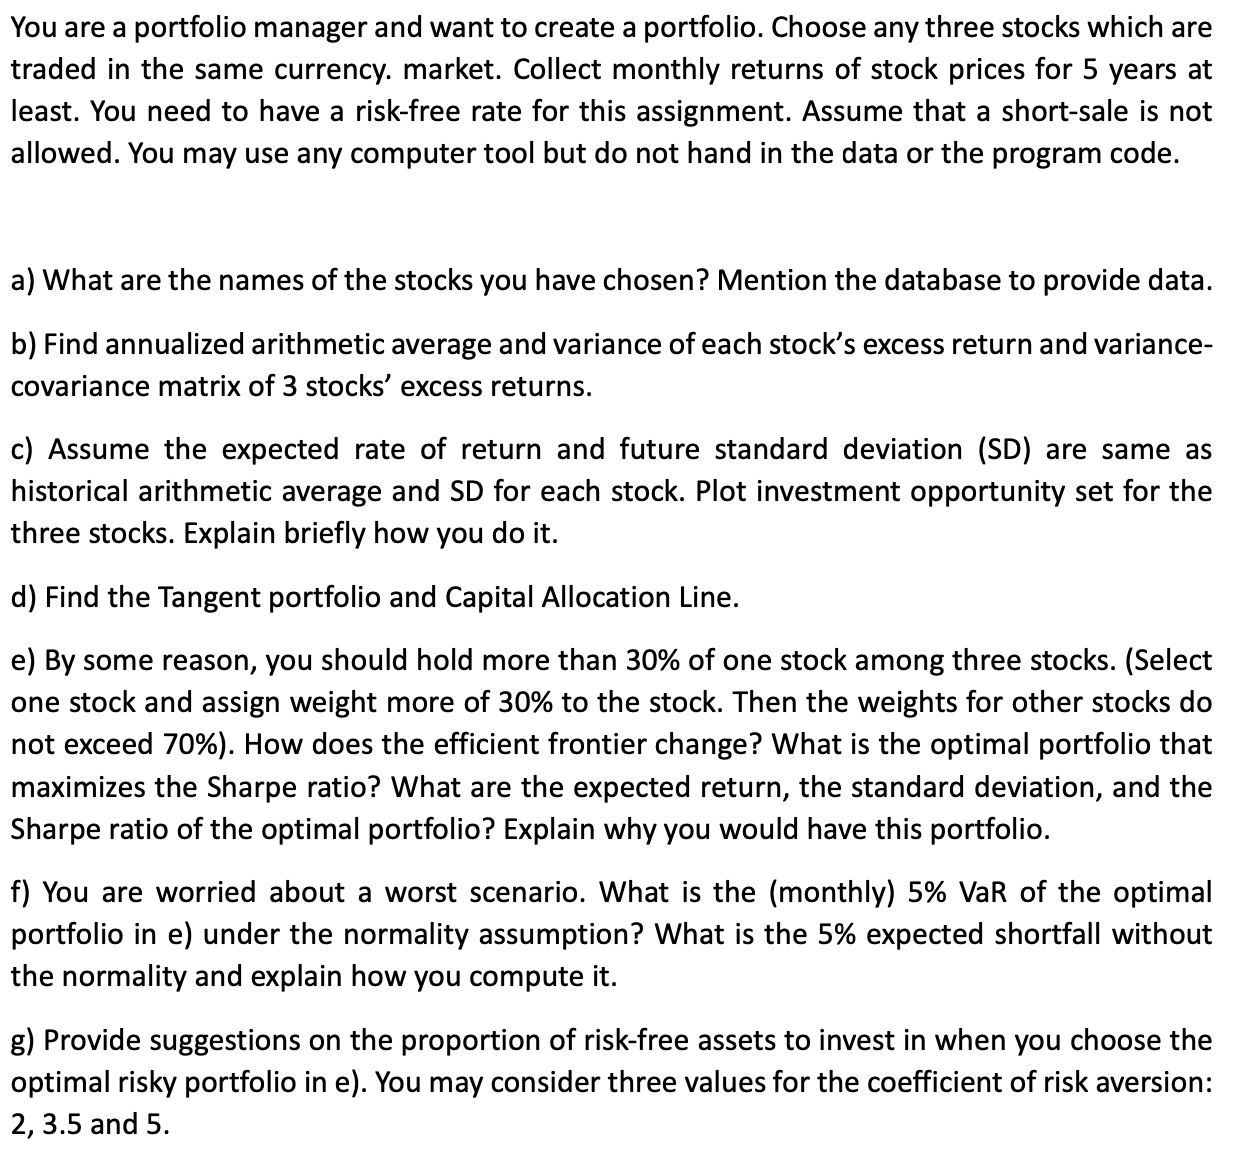
\includegraphics{images/investment_hw2.png}

\section*{Answer}\label{answer-10}
\addcontentsline{toc}{section}{Answer}

\markright{Answer}

\textbf{\emph{(a)}}

저는 \textbf{\emph{CME group(CME), ICE(ICE), Nasdaq(NDAQ)}}K 세가지
종목을 선정하였습니다.

선정 배경으로는,

\begin{enumerate}
\def\labelenumi{(\arabic{enumi})}
\tightlist
\item
  제가 거래소 산업에 관심이 많고,
\item
  세 주식 모두 미국에 상장되어있는 대표적인 글로벌 거래소이며,
\item
  동일한 거래소 산업이고 S\&P500지수의 구성종목이라 동일 선상에서
  비교하기 적합할 것으로 보이기 때문입니다.
\end{enumerate}

세 주식의 일별수정주가(Adj. close), 벤치마크지수인 S\&P500지수의
일별수정가격, 무위험이자율로 채택한 미연준의 일별 Effective-FFR(Federel
Funds Rate)를 활용하였습니다.

\begin{verbatim}
기간 : 직전 10년(2014.4 ~ 2024.3)
출처 : [Yahoo Finance](https://finance.yahoo.com/)
산출방법 :
    (월수익률) 지난달 말 대비 월말 수익률
    (월초과수익률) 월수익률 - 월말FFR/12
    (월분산) 월/월초과수익률의 표본표준편차
    (평균수익률) 월/월초과수익률을 산술평균하여 연환산 (x12)
    (평균분산) 월분산을 산술평균하여 연환산 (x12)
\end{verbatim}

\begin{Shaded}
\begin{Highlighting}[]
\FunctionTok{library}\NormalTok{(tidyverse)}
\CommentTok{\# stocks and market index S\&P500 from yahoo finance}
\NormalTok{cme }\OtherTok{\textless{}{-}} \FunctionTok{read\_csv}\NormalTok{(}\StringTok{"investment\_hw/cme.csv"}\NormalTok{) }\SpecialCharTok{\%\textgreater{}\%} \FunctionTok{tibble}\NormalTok{()}
\NormalTok{ndaq }\OtherTok{\textless{}{-}} \FunctionTok{read\_csv}\NormalTok{(}\StringTok{"investment\_hw/ndaq.csv"}\NormalTok{) }\SpecialCharTok{\%\textgreater{}\%} \FunctionTok{tibble}\NormalTok{()}
\NormalTok{ice }\OtherTok{\textless{}{-}} \FunctionTok{read\_csv}\NormalTok{(}\StringTok{"investment\_hw/ice.csv"}\NormalTok{) }\SpecialCharTok{\%\textgreater{}\%} \FunctionTok{tibble}\NormalTok{()}
\NormalTok{spx }\OtherTok{\textless{}{-}} \FunctionTok{read\_csv}\NormalTok{(}\StringTok{"investment\_hw/spx.csv"}\NormalTok{) }\SpecialCharTok{\%\textgreater{}\%} \FunctionTok{tibble}\NormalTok{()}
\CommentTok{\# risk{-}free rate is effective{-}FFR(federal funds rate)}
\NormalTok{ffr }\OtherTok{\textless{}{-}} \FunctionTok{read\_csv}\NormalTok{(}\StringTok{"investment\_hw/fedfunds.csv"}\NormalTok{) }\SpecialCharTok{\%\textgreater{}\%} \FunctionTok{tibble}\NormalTok{()}
\CommentTok{\# set period 10years}
\NormalTok{strt\_dd}\OtherTok{=}\StringTok{\textquotesingle{}20140101\textquotesingle{}}\NormalTok{; end\_dd}\OtherTok{=}\StringTok{\textquotesingle{}20240331\textquotesingle{}}
\end{Highlighting}
\end{Shaded}

\textbf{\emph{(b)}}

\begin{Shaded}
\begin{Highlighting}[]
\CommentTok{\# tidy data}
\NormalTok{raw\_data }\OtherTok{\textless{}{-}} \FunctionTok{tibble}\NormalTok{()}
\NormalTok{raw\_data }\OtherTok{\textless{}{-}}\NormalTok{ cme }\SpecialCharTok{\%\textgreater{}\%} \FunctionTok{mutate}\NormalTok{(}\AttributeTok{cme=}\StringTok{\textasciigrave{}}\AttributeTok{Adj Close}\StringTok{\textasciigrave{}}\NormalTok{) }\SpecialCharTok{\%\textgreater{}\%} \FunctionTok{select}\NormalTok{(Date,cme) }\SpecialCharTok{\%\textgreater{}\%} 
  \FunctionTok{left\_join}\NormalTok{(ndaq }\SpecialCharTok{\%\textgreater{}\%} \FunctionTok{mutate}\NormalTok{(}\AttributeTok{ndaq=}\StringTok{\textasciigrave{}}\AttributeTok{Adj Close}\StringTok{\textasciigrave{}}\NormalTok{) }\SpecialCharTok{\%\textgreater{}\%} \FunctionTok{select}\NormalTok{(Date,ndaq)) }\SpecialCharTok{\%\textgreater{}\%} 
  \FunctionTok{left\_join}\NormalTok{(ice }\SpecialCharTok{\%\textgreater{}\%} \FunctionTok{mutate}\NormalTok{(}\AttributeTok{ice=}\StringTok{\textasciigrave{}}\AttributeTok{Adj Close}\StringTok{\textasciigrave{}}\NormalTok{) }\SpecialCharTok{\%\textgreater{}\%} \FunctionTok{select}\NormalTok{(Date,ice)) }\SpecialCharTok{\%\textgreater{}\%} 
  \FunctionTok{left\_join}\NormalTok{(spx }\SpecialCharTok{\%\textgreater{}\%} \FunctionTok{mutate}\NormalTok{(}\AttributeTok{spx=}\StringTok{\textasciigrave{}}\AttributeTok{Adj Close}\StringTok{\textasciigrave{}}\NormalTok{) }\SpecialCharTok{\%\textgreater{}\%} \FunctionTok{select}\NormalTok{(Date,spx)) }\SpecialCharTok{\%\textgreater{}\%} 
  \FunctionTok{mutate}\NormalTok{(}\AttributeTok{day=}\FunctionTok{gsub}\NormalTok{(}\StringTok{"{-}"}\NormalTok{,}\StringTok{""}\NormalTok{,Date)) }\SpecialCharTok{\%\textgreater{}\%} 
  \FunctionTok{mutate}\NormalTok{(}\AttributeTok{year=}\FunctionTok{substr}\NormalTok{(day,}\DecValTok{1}\NormalTok{,}\DecValTok{4}\NormalTok{)) }\SpecialCharTok{\%\textgreater{}\%} 
  \FunctionTok{mutate}\NormalTok{(}\AttributeTok{month=}\FunctionTok{substr}\NormalTok{(day,}\DecValTok{1}\NormalTok{,}\DecValTok{6}\NormalTok{)) }\SpecialCharTok{\%\textgreater{}\%} 
  \FunctionTok{filter}\NormalTok{(day}\SpecialCharTok{\textgreater{}=}\NormalTok{strt\_dd,day}\SpecialCharTok{\textless{}=}\NormalTok{end\_dd) }\SpecialCharTok{\%\textgreater{}\%} 
  \FunctionTok{left\_join}\NormalTok{(ffr }\SpecialCharTok{\%\textgreater{}\%} 
              \FunctionTok{mutate}\NormalTok{(}\AttributeTok{ffr=}\NormalTok{FEDFUNDS}\SpecialCharTok{/}\DecValTok{100}\NormalTok{,}
                     \AttributeTok{month=}\FunctionTok{substr}\NormalTok{(}\FunctionTok{gsub}\NormalTok{(}\StringTok{"{-}"}\NormalTok{,}\StringTok{""}\NormalTok{,}\FunctionTok{as.character}\NormalTok{(DATE)),}\DecValTok{1}\NormalTok{,}\DecValTok{6}\NormalTok{)) }\SpecialCharTok{\%\textgreater{}\%} 
              \FunctionTok{select}\NormalTok{(month,ffr)) }\SpecialCharTok{\%\textgreater{}\%} 
  \FunctionTok{select}\NormalTok{(year,month,day,cme,ndaq,ice,spx,ffr,Date)}
\CommentTok{\# using monthly return}
\NormalTok{monthly\_raw }\OtherTok{\textless{}{-}} \FunctionTok{tibble}\NormalTok{()}
\NormalTok{monthly\_raw }\OtherTok{\textless{}{-}}\NormalTok{ raw\_data }\SpecialCharTok{\%\textgreater{}\%} 
  \FunctionTok{group\_by}\NormalTok{(year,month) }\SpecialCharTok{\%\textgreater{}\%} 
  \FunctionTok{arrange}\NormalTok{(day }\SpecialCharTok{\%\textgreater{}\%} \FunctionTok{desc}\NormalTok{()) }\SpecialCharTok{\%\textgreater{}\%} 
  \FunctionTok{slice}\NormalTok{(}\DecValTok{1}\NormalTok{) }\SpecialCharTok{\%\textgreater{}\%} 
  \FunctionTok{pivot\_longer}\NormalTok{(.,}\FunctionTok{c}\NormalTok{(}\StringTok{"cme"}\NormalTok{,}\StringTok{"ndaq"}\NormalTok{,}\StringTok{"ice"}\NormalTok{,}\StringTok{"spx"}\NormalTok{),}
               \AttributeTok{names\_to =} \StringTok{"name"}\NormalTok{,}\AttributeTok{values\_to =} \StringTok{"price"}\NormalTok{) }\SpecialCharTok{\%\textgreater{}\%} 
  \FunctionTok{ungroup}\NormalTok{() }\SpecialCharTok{\%\textgreater{}\%} 
  \FunctionTok{arrange}\NormalTok{(name,year,month) }\SpecialCharTok{\%\textgreater{}\%} 
  \FunctionTok{mutate}\NormalTok{(}\AttributeTok{return=}\NormalTok{price}\SpecialCharTok{/}\FunctionTok{lag}\NormalTok{(price)}\SpecialCharTok{{-}}\DecValTok{1}\NormalTok{) }\SpecialCharTok{\%\textgreater{}\%}  \CommentTok{\# monthly return}
  \FunctionTok{mutate}\NormalTok{(}\AttributeTok{excess\_return=}\NormalTok{return}\SpecialCharTok{{-}}\NormalTok{ffr}\SpecialCharTok{*}\NormalTok{(}\DecValTok{1}\SpecialCharTok{/}\DecValTok{12}\NormalTok{)) }\SpecialCharTok{\%\textgreater{}\%} 
  \FunctionTok{filter}\NormalTok{(}\FunctionTok{as.integer}\NormalTok{(month)}\SpecialCharTok{\textgreater{}=}\DecValTok{201404}\NormalTok{)}

\CommentTok{\# calculate arithmatic mean\&var and var{-}cov matrix of excess return of stocks}
\NormalTok{monthly\_stat }\OtherTok{\textless{}{-}} \FunctionTok{tibble}\NormalTok{()}
\NormalTok{monthly\_stat }\OtherTok{\textless{}{-}}\NormalTok{ monthly\_raw }\SpecialCharTok{\%\textgreater{}\%} 
  \FunctionTok{ungroup}\NormalTok{() }\SpecialCharTok{\%\textgreater{}\%} 
  \FunctionTok{group\_by}\NormalTok{(name) }\SpecialCharTok{\%\textgreater{}\%} 
  \FunctionTok{summarise}\NormalTok{(}\AttributeTok{avg\_excess=}\FunctionTok{mean}\NormalTok{(excess\_return)}\SpecialCharTok{*}\DecValTok{12}\NormalTok{,}
            \AttributeTok{var\_excess=}\FunctionTok{sd}\NormalTok{(excess\_return)}\SpecialCharTok{\^{}}\DecValTok{2}\SpecialCharTok{*}\DecValTok{12}\NormalTok{,}
            \AttributeTok{avg\_return=}\FunctionTok{mean}\NormalTok{(return)}\SpecialCharTok{*}\DecValTok{12}\NormalTok{,}
            \AttributeTok{var\_return=}\FunctionTok{sd}\NormalTok{(return)}\SpecialCharTok{\^{}}\DecValTok{2}\SpecialCharTok{*}\DecValTok{12}\NormalTok{,}
            \AttributeTok{avg\_rf=}\FunctionTok{mean}\NormalTok{(ffr)) }\CommentTok{\# Annualized}
\CommentTok{\# Cov matrix}
\NormalTok{variance\_matrix }\OtherTok{\textless{}{-}}\NormalTok{ monthly\_raw }\SpecialCharTok{\%\textgreater{}\%} 
  \FunctionTok{ungroup}\NormalTok{() }\SpecialCharTok{\%\textgreater{}\%}
  \FunctionTok{select}\NormalTok{(month,name,excess\_return) }\SpecialCharTok{\%\textgreater{}\%} 
  \FunctionTok{pivot\_wider}\NormalTok{(}\AttributeTok{names\_from =} \StringTok{"name"}\NormalTok{, }\AttributeTok{values\_from =} \StringTok{"excess\_return"}\NormalTok{) }\SpecialCharTok{\%\textgreater{}\%} 
  \FunctionTok{select}\NormalTok{(cme,ice,ndaq,spx) }\SpecialCharTok{\%\textgreater{}\%} 
  \FunctionTok{var}\NormalTok{()}
\CommentTok{\# Corr matrix}
\NormalTok{cor\_matrix }\OtherTok{\textless{}{-}}\NormalTok{ monthly\_raw }\SpecialCharTok{\%\textgreater{}\%} 
  \FunctionTok{ungroup}\NormalTok{() }\SpecialCharTok{\%\textgreater{}\%}
  \FunctionTok{select}\NormalTok{(month,name,excess\_return) }\SpecialCharTok{\%\textgreater{}\%} 
  \FunctionTok{pivot\_wider}\NormalTok{(}\AttributeTok{names\_from =} \StringTok{"name"}\NormalTok{, }\AttributeTok{values\_from =} \StringTok{"excess\_return"}\NormalTok{) }\SpecialCharTok{\%\textgreater{}\%} 
  \FunctionTok{select}\NormalTok{(cme,ice,ndaq,spx) }\SpecialCharTok{\%\textgreater{}\%} 
  \FunctionTok{cor}\NormalTok{()}
\end{Highlighting}
\end{Shaded}

위 방법을 기준으로 산출한 각 주식의 평균초과수익률(연환산) 및
공분산행렬은 아래와 같습니다.

\textbf{Excess return : CME 15.0\%, ICE 14.4\%, Nasdaq 18.8\%}

\begin{Shaded}
\begin{Highlighting}[]
\NormalTok{monthly\_stat}
\end{Highlighting}
\end{Shaded}

\begin{verbatim}
# A tibble: 4 x 6
  name  avg_excess var_excess avg_return var_return avg_rf
  <chr>      <dbl>      <dbl>      <dbl>      <dbl>  <dbl>
1 cme        0.150     0.0340      0.165     0.0340 0.0141
2 ice        0.144     0.0414      0.158     0.0415 0.0141
3 ndaq       0.188     0.0415      0.202     0.0413 0.0141
4 spx        0.101     0.0229      0.115     0.0229 0.0141
\end{verbatim}

\textbf{Variance-Covariance Matrix of three stocks\&Benchmark index}

\begin{Shaded}
\begin{Highlighting}[]
\NormalTok{variance\_matrix}
\end{Highlighting}
\end{Shaded}

\begin{verbatim}
              cme         ice        ndaq          spx
cme  0.0028310476 0.001767299 0.001138796 0.0008194417
ice  0.0017672988 0.003452184 0.002149990 0.0016652315
ndaq 0.0011387956 0.002149990 0.003456322 0.0016308630
spx  0.0008194417 0.001665231 0.001630863 0.0019071007
\end{verbatim}

\textbf{Correlation Matrix of three stocks\&Benchmark index}

\begin{Shaded}
\begin{Highlighting}[]
\NormalTok{cor\_matrix}
\end{Highlighting}
\end{Shaded}

\begin{verbatim}
           cme       ice      ndaq       spx
cme  1.0000000 0.5653136 0.3640534 0.3526612
ice  0.5653136 1.0000000 0.6224185 0.6489942
ndaq 0.3640534 0.6224185 1.0000000 0.6352191
spx  0.3526612 0.6489942 0.6352191 1.0000000
\end{verbatim}

\textbf{\emph{(c)}}

각 주식의 기대수익률과 미래변동성이 과거실현값과 동일하다고
가정하겠습니다.

공매도는 없다고 가정하였으므로 각 주식의 비중이 양수가 되도록 설정하고,
먼저 두개의 주식으로 구성된 포트폴리오의 efficient frontier를 각각
구하도록 하겠습니다.

그 다음, 하나의 주식과 다른 두 주식의 포트폴리오를 재결합하면 새로운
포트폴리오를 구성할 수 있으며, 이를 반복하여 efficient frontier를
도식화할 수 있습니다.

아래 코드에서는 ICE의 구성비중을 5\%, 10\%, \ldots{} , 95\%로 고정하고
CME-Nasdaq 포트폴리오와 재결합을 반복하여 efficient frontier를
구현하였습니다.

\begin{Shaded}
\begin{Highlighting}[]
\CommentTok{\# Portfolio return/vol of variance combinations three stocks}
\NormalTok{portfolio }\OtherTok{\textless{}{-}} \FunctionTok{tibble}\NormalTok{()}
\NormalTok{portfolio }\OtherTok{\textless{}{-}} \FunctionTok{tibble}\NormalTok{(}\AttributeTok{cme=}\FunctionTok{seq}\NormalTok{(}\DecValTok{0}\NormalTok{,}\DecValTok{1}\NormalTok{,}\FloatTok{0.002}\NormalTok{),}\AttributeTok{ice=}\FunctionTok{seq}\NormalTok{(}\DecValTok{1}\NormalTok{,}\DecValTok{0}\NormalTok{,}\SpecialCharTok{{-}}\FloatTok{0.002}\NormalTok{)) }\SpecialCharTok{\%\textgreater{}\%} 
  \FunctionTok{union\_all}\NormalTok{(.,}\FunctionTok{tibble}\NormalTok{(}\AttributeTok{cme=}\FunctionTok{seq}\NormalTok{(}\DecValTok{0}\NormalTok{,}\DecValTok{1}\NormalTok{,}\FloatTok{0.002}\NormalTok{),}\AttributeTok{ice=}\DecValTok{0}\NormalTok{)) }\SpecialCharTok{\%\textgreater{}\%} 
  \FunctionTok{union\_all}\NormalTok{(.,}\FunctionTok{tibble}\NormalTok{(}\AttributeTok{cme=}\DecValTok{0}\NormalTok{,}\AttributeTok{ice=}\FunctionTok{seq}\NormalTok{(}\DecValTok{1}\NormalTok{,}\DecValTok{0}\NormalTok{,}\SpecialCharTok{{-}}\FloatTok{0.002}\NormalTok{)))}

\ControlFlowTok{for}\NormalTok{(i }\ControlFlowTok{in} \FunctionTok{seq}\NormalTok{(}\FloatTok{0.05}\NormalTok{,}\FloatTok{0.95}\NormalTok{,}\FloatTok{0.05}\NormalTok{))\{portfolio }\OtherTok{\textless{}{-}}\NormalTok{ portfolio }\SpecialCharTok{\%\textgreater{}\%}
  \FunctionTok{union\_all}\NormalTok{(.,}\FunctionTok{tibble}\NormalTok{(}\AttributeTok{cme=}\FunctionTok{seq}\NormalTok{(}\DecValTok{0}\NormalTok{,}\DecValTok{1}\SpecialCharTok{{-}}\NormalTok{i,}\FloatTok{0.005}\NormalTok{),}\AttributeTok{ice=}\NormalTok{i))\}}
\ControlFlowTok{for}\NormalTok{(i }\ControlFlowTok{in} \FunctionTok{seq}\NormalTok{(}\FloatTok{0.25}\NormalTok{,}\FloatTok{0.30}\NormalTok{,}\FloatTok{0.01}\NormalTok{))\{portfolio }\OtherTok{\textless{}{-}}\NormalTok{ portfolio }\SpecialCharTok{\%\textgreater{}\%}
  \FunctionTok{union\_all}\NormalTok{(.,}\FunctionTok{tibble}\NormalTok{(}\AttributeTok{cme=}\FunctionTok{seq}\NormalTok{(}\DecValTok{0}\NormalTok{,}\DecValTok{1}\SpecialCharTok{{-}}\NormalTok{i,}\FloatTok{0.005}\NormalTok{),}\AttributeTok{ice=}\NormalTok{i))\}}

\NormalTok{portfolio }\OtherTok{\textless{}{-}}\NormalTok{ portfolio }\SpecialCharTok{\%\textgreater{}\%} 
  \FunctionTok{mutate}\NormalTok{(}\AttributeTok{ndaq=}\DecValTok{1}\SpecialCharTok{{-}}\NormalTok{cme}\SpecialCharTok{{-}}\NormalTok{ice) }\SpecialCharTok{\%\textgreater{}\%} 
  \FunctionTok{mutate}\NormalTok{(}\AttributeTok{return=}\NormalTok{cme}\SpecialCharTok{*}\NormalTok{monthly\_stat}\SpecialCharTok{$}\NormalTok{avg\_return[}\DecValTok{1}\NormalTok{]}
         \SpecialCharTok{+}\NormalTok{ice}\SpecialCharTok{*}\NormalTok{monthly\_stat}\SpecialCharTok{$}\NormalTok{avg\_return[}\DecValTok{2}\NormalTok{]}
         \SpecialCharTok{+}\NormalTok{ndaq}\SpecialCharTok{*}\NormalTok{monthly\_stat}\SpecialCharTok{$}\NormalTok{avg\_return[}\DecValTok{3}\NormalTok{],}
         \AttributeTok{vol=}\FunctionTok{sqrt}\NormalTok{(cme}\SpecialCharTok{\^{}}\DecValTok{2}\SpecialCharTok{*}\NormalTok{monthly\_stat}\SpecialCharTok{$}\NormalTok{var\_return[}\DecValTok{1}\NormalTok{]}
                  \SpecialCharTok{+}\NormalTok{ice}\SpecialCharTok{\^{}}\DecValTok{2}\SpecialCharTok{*}\NormalTok{monthly\_stat}\SpecialCharTok{$}\NormalTok{var\_return[}\DecValTok{2}\NormalTok{]}
                  \SpecialCharTok{+}\NormalTok{ndaq}\SpecialCharTok{\^{}}\DecValTok{2}\SpecialCharTok{*}\NormalTok{monthly\_stat}\SpecialCharTok{$}\NormalTok{var\_return[}\DecValTok{3}\NormalTok{]}
                  \SpecialCharTok{+}\DecValTok{2}\SpecialCharTok{*}\NormalTok{cme}\SpecialCharTok{*}\NormalTok{ice}\SpecialCharTok{*}\NormalTok{variance\_matrix[}\DecValTok{2}\NormalTok{]}
                  \SpecialCharTok{+}\DecValTok{2}\SpecialCharTok{*}\NormalTok{cme}\SpecialCharTok{*}\NormalTok{ndaq}\SpecialCharTok{*}\NormalTok{variance\_matrix[}\DecValTok{3}\NormalTok{]}
                  \SpecialCharTok{+}\DecValTok{2}\SpecialCharTok{*}\NormalTok{ndaq}\SpecialCharTok{*}\NormalTok{ice}\SpecialCharTok{*}\NormalTok{variance\_matrix[}\DecValTok{7}\NormalTok{])) }\SpecialCharTok{\%\textgreater{}\%} 
  \FunctionTok{mutate}\NormalTok{(}\AttributeTok{sharpe=}\NormalTok{(return}\SpecialCharTok{{-}}\NormalTok{monthly\_stat}\SpecialCharTok{$}\NormalTok{avg\_rf[}\DecValTok{1}\NormalTok{])}\SpecialCharTok{/}\NormalTok{vol)}

\NormalTok{plot\_portfolio }\OtherTok{\textless{}{-}} \FunctionTok{ggplot}\NormalTok{(}\AttributeTok{data=}\NormalTok{portfolio,}\AttributeTok{mapping=}\FunctionTok{aes}\NormalTok{(}\AttributeTok{x=}\NormalTok{vol,}\AttributeTok{y=}\NormalTok{return))}\SpecialCharTok{+}
  \FunctionTok{geom\_point}\NormalTok{(}\AttributeTok{data=}\NormalTok{portfolio }\SpecialCharTok{\%\textgreater{}\%} \FunctionTok{filter}\NormalTok{(ndaq}\SpecialCharTok{==}\DecValTok{0}\NormalTok{),}\AttributeTok{size=}\FloatTok{0.5}\NormalTok{,}\AttributeTok{color=}\StringTok{"red"}\NormalTok{)}\SpecialCharTok{+}
  \FunctionTok{geom\_point}\NormalTok{(}\AttributeTok{data=}\NormalTok{portfolio }\SpecialCharTok{\%\textgreater{}\%} \FunctionTok{filter}\NormalTok{(ice}\SpecialCharTok{==}\DecValTok{0}\NormalTok{),}\AttributeTok{size=}\FloatTok{0.5}\NormalTok{,}\AttributeTok{color=}\StringTok{"blue"}\NormalTok{)}\SpecialCharTok{+}
  \FunctionTok{geom\_point}\NormalTok{(}\AttributeTok{data=}\NormalTok{portfolio }\SpecialCharTok{\%\textgreater{}\%} \FunctionTok{filter}\NormalTok{(cme}\SpecialCharTok{==}\DecValTok{0}\NormalTok{),}\AttributeTok{size=}\FloatTok{0.5}\NormalTok{,}\AttributeTok{color=}\StringTok{"green"}\NormalTok{)}\SpecialCharTok{+}
  \FunctionTok{scale\_x\_continuous}\NormalTok{(}\AttributeTok{limits=}\FunctionTok{c}\NormalTok{(}\FloatTok{0.08}\NormalTok{,}\FloatTok{0.22}\NormalTok{))}\SpecialCharTok{+}
  \FunctionTok{scale\_y\_continuous}\NormalTok{(}\AttributeTok{limits=}\FunctionTok{c}\NormalTok{(}\FloatTok{0.15}\NormalTok{,}\FloatTok{0.21}\NormalTok{))}\SpecialCharTok{+}
  \FunctionTok{labs}\NormalTok{(}\AttributeTok{title =} \StringTok{"Invest Opportunity of three stocks"}\NormalTok{,}
       \AttributeTok{x=}\StringTok{"standard deviation"}\NormalTok{,}\AttributeTok{y=}\StringTok{"expected return"}\NormalTok{) }\SpecialCharTok{+}
  \FunctionTok{annotate}\NormalTok{(}\AttributeTok{geom=}\StringTok{"text"}\NormalTok{,}\AttributeTok{x=}\FloatTok{0.182}\NormalTok{,}\AttributeTok{y=}\FloatTok{0.17}\NormalTok{,}\AttributeTok{label=}\StringTok{"CME"}\NormalTok{)}\SpecialCharTok{+}
  \FunctionTok{annotate}\NormalTok{(}\AttributeTok{geom=}\StringTok{"text"}\NormalTok{,}\AttributeTok{x=}\FloatTok{0.202}\NormalTok{,}\AttributeTok{y=}\FloatTok{0.205}\NormalTok{,}\AttributeTok{label=}\StringTok{"Nasdaq"}\NormalTok{)}\SpecialCharTok{+}
  \FunctionTok{annotate}\NormalTok{(}\AttributeTok{geom=}\StringTok{"text"}\NormalTok{,}\AttributeTok{x=}\FloatTok{0.202}\NormalTok{,}\AttributeTok{y=}\FloatTok{0.162}\NormalTok{,}\AttributeTok{label=}\StringTok{"ICE"}\NormalTok{)}\SpecialCharTok{+}
  \FunctionTok{theme\_bw}\NormalTok{()}

\NormalTok{plot\_combination }\OtherTok{\textless{}{-}}\NormalTok{ plot\_portfolio }\SpecialCharTok{+}
  \FunctionTok{geom\_point}\NormalTok{(}\AttributeTok{data=}\NormalTok{portfolio }\SpecialCharTok{\%\textgreater{}\%} \FunctionTok{filter}\NormalTok{(cme}\SpecialCharTok{!=}\DecValTok{0}\SpecialCharTok{\&}\NormalTok{ice}\SpecialCharTok{!=}\DecValTok{0}\SpecialCharTok{\&}\NormalTok{ndaq}\SpecialCharTok{!=}\DecValTok{0}\NormalTok{),}\AttributeTok{size=}\DecValTok{1}\NormalTok{,}
  \AttributeTok{color=}\StringTok{"black"}\NormalTok{,}\AttributeTok{alpha=}\FloatTok{0.1}\NormalTok{)}

\NormalTok{plot\_combination}
\end{Highlighting}
\end{Shaded}

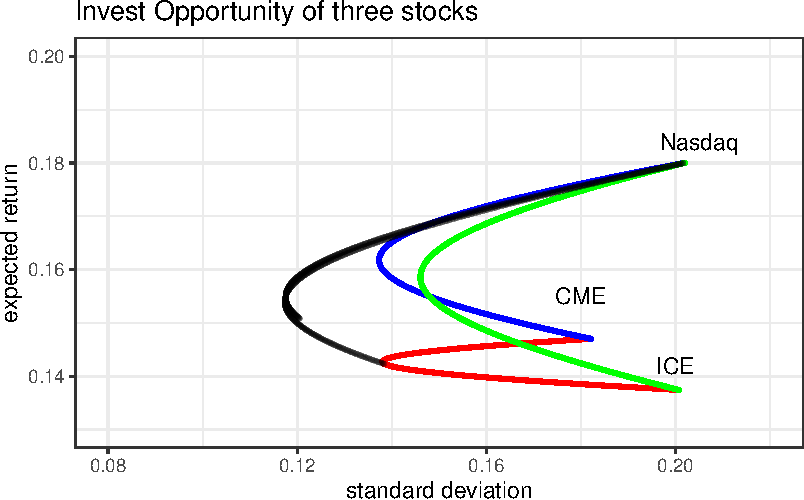
\includegraphics{investment_hw2_files/figure-pdf/unnamed-chunk-6-1.pdf}

\textbf{\emph{(d)}}

Tangent p/f는 Sharpe r/o를 최대화시키는 세 주식의 조합으로, 위에서
도식화한 투자기회에 대하여 무위험이자율을 y절편으로 가지는 접선을 그려서
시각화할 수 있습니다.

접선의 기울기는 포트폴리오의 초과수익률을 변동성으로 나눈 값으로 Sharpe
r/o가 되므로, 이 접선이 CAL에 해당합니다.

\begin{Shaded}
\begin{Highlighting}[]
\NormalTok{sharpe}\OtherTok{=}\FunctionTok{max}\NormalTok{(portfolio}\SpecialCharTok{$}\NormalTok{sharpe)}
\NormalTok{tangent }\OtherTok{\textless{}{-}} \FunctionTok{tibble}\NormalTok{(}\AttributeTok{vol=}\FunctionTok{seq}\NormalTok{(}\FloatTok{0.08}\NormalTok{,}\FloatTok{0.17}\NormalTok{,}\FloatTok{0.01}\NormalTok{)) }\SpecialCharTok{\%\textgreater{}\%} 
  \FunctionTok{mutate}\NormalTok{(}\AttributeTok{return=}\NormalTok{monthly\_stat}\SpecialCharTok{$}\NormalTok{avg\_rf[}\DecValTok{1}\NormalTok{]}\SpecialCharTok{+}\NormalTok{sharpe}\SpecialCharTok{*}\NormalTok{vol)}

\NormalTok{plot\_tangent }\OtherTok{\textless{}{-}}\NormalTok{ plot\_combination}\SpecialCharTok{+}
  \FunctionTok{geom\_line}\NormalTok{(}\AttributeTok{data=}\NormalTok{tangent)}\SpecialCharTok{+}
  \FunctionTok{scale\_x\_continuous}\NormalTok{(}\AttributeTok{limits=}\FunctionTok{c}\NormalTok{(}\FloatTok{0.04}\NormalTok{,}\FloatTok{0.26}\NormalTok{))}\SpecialCharTok{+}
  \FunctionTok{scale\_y\_continuous}\NormalTok{(}\AttributeTok{limits=}\FunctionTok{c}\NormalTok{(}\FloatTok{0.11}\NormalTok{,}\FloatTok{0.25}\NormalTok{))}\SpecialCharTok{+}
  \FunctionTok{annotate}\NormalTok{(}\AttributeTok{geom=}\StringTok{"text"}\NormalTok{,}\AttributeTok{x=}\FloatTok{0.125}\NormalTok{,}\AttributeTok{y=}\FloatTok{0.23}\NormalTok{,}\AttributeTok{label=}\StringTok{"CAL, y=1.3667x+0.0141"}\NormalTok{)}\SpecialCharTok{+}
  \FunctionTok{annotate}\NormalTok{(}\AttributeTok{geom=}\StringTok{"text"}\NormalTok{,}\AttributeTok{x=}\FloatTok{0.125}\NormalTok{,}\AttributeTok{y=}\FloatTok{0.22}\NormalTok{,}\AttributeTok{label=}\StringTok{"sharpe r/o=1.3667"}\NormalTok{)}\SpecialCharTok{+}
  \FunctionTok{annotate}\NormalTok{(}\AttributeTok{geom=}\StringTok{"text"}\NormalTok{,}\AttributeTok{x=}\FloatTok{0.1}\NormalTok{,}\AttributeTok{y=}\FloatTok{0.18}\NormalTok{,}\AttributeTok{label=}\StringTok{"Tangent p/f"}\NormalTok{)}
\end{Highlighting}
\end{Shaded}

\begin{verbatim}
Scale for x is already present.
Adding another scale for x, which will replace the existing scale.
Scale for y is already present.
Adding another scale for y, which will replace the existing scale.
\end{verbatim}

\begin{Shaded}
\begin{Highlighting}[]
\NormalTok{plot\_tangent}
\end{Highlighting}
\end{Shaded}

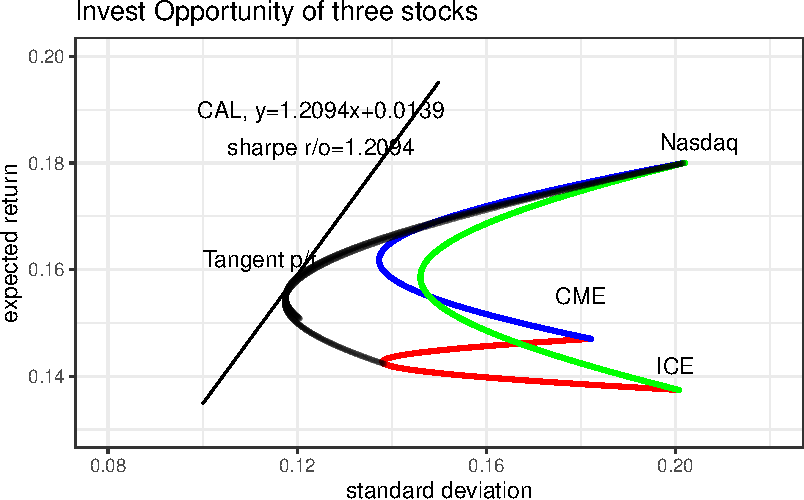
\includegraphics{investment_hw2_files/figure-pdf/unnamed-chunk-7-1.pdf}

이 때, Tangent p/f의 기대수익률/변동성/구성비율은 아래와 같습니다.

\begin{Shaded}
\begin{Highlighting}[]
\NormalTok{portfolio }\SpecialCharTok{\%\textgreater{}\%} \FunctionTok{arrange}\NormalTok{(sharpe }\SpecialCharTok{\%\textgreater{}\%} \FunctionTok{desc}\NormalTok{()) }\SpecialCharTok{\%\textgreater{}\%} \FunctionTok{slice}\NormalTok{(}\DecValTok{1}\NormalTok{)}
\end{Highlighting}
\end{Shaded}

\begin{verbatim}
# A tibble: 1 x 6
    cme   ice  ndaq return   vol sharpe
  <dbl> <dbl> <dbl>  <dbl> <dbl>  <dbl>
1  0.36  0.27  0.37  0.177 0.119   1.37
\end{verbatim}

\textbf{\emph{(e)}}

Tangent p/f에서 CME, Nasdaq의 비중은 각각 36\%, 37\%로 이미 30\%를
초과하였습니다. 따라서 30\%를 초과보유할 주식을 선정할 때 두 주식을
선정한다면 최적포트폴리오는 (d)의 Tangent p/f와 동일할 것 입니다.

한편, ICE를 선정한다면 (d)의 Tangent p/f 구성이 불가능합니다. 이 경우
새로운 efficient frontier는 아래와 같이 도식화할 수 있으며, 새로운
최적포트폴리오는 ICE의 비중이 정확히 30\%일 때 결정됩니다.

\begin{Shaded}
\begin{Highlighting}[]
\CommentTok{\# Set ice\textgreater{}=0.3}
\NormalTok{portfolio2 }\OtherTok{\textless{}{-}}\NormalTok{ portfolio }\SpecialCharTok{\%\textgreater{}\%} \FunctionTok{filter}\NormalTok{(ice}\SpecialCharTok{\textgreater{}=}\FloatTok{0.3}\NormalTok{)}
\NormalTok{sharpe2}\OtherTok{=}\FunctionTok{max}\NormalTok{(portfolio2}\SpecialCharTok{$}\NormalTok{sharpe)}
\NormalTok{tangent2 }\OtherTok{\textless{}{-}} \FunctionTok{tibble}\NormalTok{(}\AttributeTok{vol=}\FunctionTok{seq}\NormalTok{(}\FloatTok{0.1}\NormalTok{,}\FloatTok{0.14}\NormalTok{,}\FloatTok{0.01}\NormalTok{)) }\SpecialCharTok{\%\textgreater{}\%} 
  \FunctionTok{mutate}\NormalTok{(}\AttributeTok{return=}\NormalTok{monthly\_stat}\SpecialCharTok{$}\NormalTok{avg\_rf[}\DecValTok{1}\NormalTok{]}\SpecialCharTok{+}\NormalTok{sharpe2}\SpecialCharTok{*}\NormalTok{vol)}

\NormalTok{portfolio2 }\SpecialCharTok{\%\textgreater{}\%} \FunctionTok{arrange}\NormalTok{(}\FunctionTok{desc}\NormalTok{(sharpe))}
\end{Highlighting}
\end{Shaded}

\begin{verbatim}
# A tibble: 1,905 x 6
     cme   ice  ndaq return   vol sharpe
   <dbl> <dbl> <dbl>  <dbl> <dbl>  <dbl>
 1 0.34    0.3 0.36   0.176 0.119   1.36
 2 0.34    0.3 0.36   0.176 0.119   1.36
 3 0.345   0.3 0.355  0.176 0.119   1.36
 4 0.345   0.3 0.355  0.176 0.119   1.36
 5 0.335   0.3 0.365  0.176 0.119   1.36
 6 0.335   0.3 0.365  0.176 0.119   1.36
 7 0.35    0.3 0.35   0.176 0.119   1.36
 8 0.35    0.3 0.35   0.176 0.119   1.36
 9 0.33    0.3 0.37   0.176 0.119   1.36
10 0.33    0.3 0.37   0.176 0.119   1.36
# i 1,895 more rows
\end{verbatim}

\begin{Shaded}
\begin{Highlighting}[]
\NormalTok{plot\_tangent2 }\OtherTok{\textless{}{-}}\NormalTok{ plot\_portfolio }\SpecialCharTok{+}
  \FunctionTok{geom\_point}\NormalTok{(}\AttributeTok{data=}\NormalTok{portfolio2 }\SpecialCharTok{\%\textgreater{}\%} \FunctionTok{filter}\NormalTok{(cme}\SpecialCharTok{!=}\DecValTok{0}\SpecialCharTok{\&}\NormalTok{ice}\SpecialCharTok{!=}\DecValTok{0}\SpecialCharTok{\&}\NormalTok{ndaq}\SpecialCharTok{!=}\DecValTok{0}\NormalTok{),}
             \AttributeTok{size=}\DecValTok{1}\NormalTok{,}\AttributeTok{color=}\StringTok{"black"}\NormalTok{,}\AttributeTok{alpha=}\FloatTok{0.2}\NormalTok{)}\SpecialCharTok{+}
  \FunctionTok{geom\_line}\NormalTok{(}\AttributeTok{data=}\NormalTok{tangent2)}\SpecialCharTok{+}
  \FunctionTok{annotate}\NormalTok{(}\AttributeTok{geom=}\StringTok{"text"}\NormalTok{,}\AttributeTok{x=}\FloatTok{0.117}\NormalTok{,}\AttributeTok{y=}\FloatTok{0.2}\NormalTok{,}\AttributeTok{label=}\StringTok{"CAL, y=1.3639x+0.0141"}\NormalTok{)}\SpecialCharTok{+}
  \FunctionTok{annotate}\NormalTok{(}\AttributeTok{geom=}\StringTok{"text"}\NormalTok{,}\AttributeTok{x=}\FloatTok{0.117}\NormalTok{,}\AttributeTok{y=}\FloatTok{0.193}\NormalTok{,}\AttributeTok{label=}\StringTok{"sharpe r/o=1.3639"}\NormalTok{)}\SpecialCharTok{+}
  \FunctionTok{annotate}\NormalTok{(}\AttributeTok{geom=}\StringTok{"text"}\NormalTok{,}\AttributeTok{x=}\FloatTok{0.11}\NormalTok{,}\AttributeTok{y=}\FloatTok{0.18}\NormalTok{,}\AttributeTok{label=}\StringTok{"Optimal p/f"}\NormalTok{)}
\NormalTok{plot\_tangent2}
\end{Highlighting}
\end{Shaded}

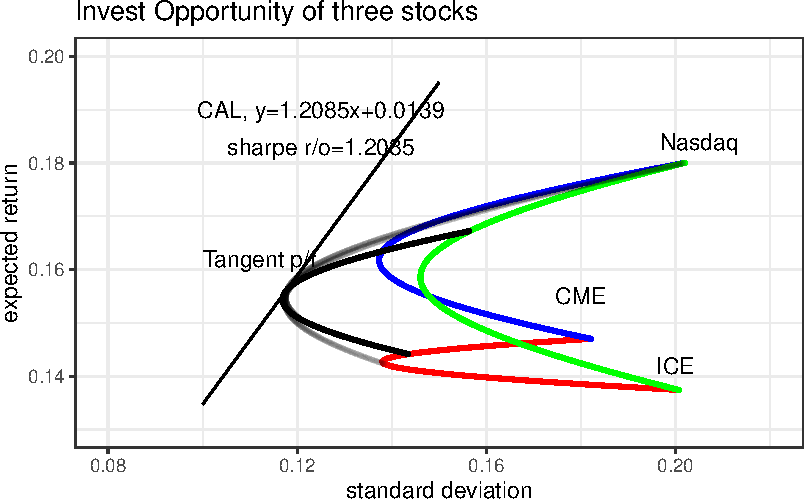
\includegraphics{investment_hw2_files/figure-pdf/unnamed-chunk-9-1.pdf}

\textbf{Optimal p/f의 기대수익률/변동성/구성비율}은 아래와 같습니다.

\begin{Shaded}
\begin{Highlighting}[]
\NormalTok{optimal }\OtherTok{\textless{}{-}}\NormalTok{ portfolio2 }\SpecialCharTok{\%\textgreater{}\%} \FunctionTok{arrange}\NormalTok{(sharpe }\SpecialCharTok{\%\textgreater{}\%} \FunctionTok{desc}\NormalTok{()) }\SpecialCharTok{\%\textgreater{}\%} \FunctionTok{slice}\NormalTok{(}\DecValTok{1}\NormalTok{)}
\NormalTok{optimal}
\end{Highlighting}
\end{Shaded}

\begin{verbatim}
# A tibble: 1 x 6
    cme   ice  ndaq return   vol sharpe
  <dbl> <dbl> <dbl>  <dbl> <dbl>  <dbl>
1  0.34   0.3  0.36  0.176 0.119   1.36
\end{verbatim}

\textbf{\emph{(f)}}

먼저, 포트폴리오의 연환산수익률이 정규분포를 따른다면 표준정규분포표를
참조하여 \textbf{Value at Risk를 다음과 같이 산출}할 수 있습니다.

\[5\%\;VaR=E(r_p)-1.65\sigma_p=0.176-1.65\times 0.119=-1.99\%\]

\begin{Shaded}
\begin{Highlighting}[]
\NormalTok{VaR}\OtherTok{=}\NormalTok{optimal}\SpecialCharTok{$}\NormalTok{return}\FloatTok{{-}1.65}\SpecialCharTok{*}\NormalTok{optimal}\SpecialCharTok{$}\NormalTok{vol; VaR}
\end{Highlighting}
\end{Shaded}

\begin{verbatim}
[1] -0.01990571
\end{verbatim}

만약 수익률의 분포가 정규분포가 아니라면, Historical VaR 및 ES(Expected
Shortfall)을 산출할 수 있습니다. 이를 데이터의 참조기간인 \textbf{과거
10년간 최적포트폴리오의 월수익률이 필요}합니다.

위의 최적포트폴리오는 \textbf{CME 34\%, ICE 30\%, Nasdaq 36\%로 구성된
포트폴리오}이므로, 거래비용 등을 무시하고 매월말 포트폴리오의 구성비율을
조정한다고 가정하고 포트폴리오의 명목금액을 \(P_t\), 각 주식의
\((t,t+1)\) 월수익률을 \(r_{t,k}\)라고 한다면 \((t,t+1)\)간 포트폴리오의
월수익률 \(r_t\)는 다음과 같습니다.

\[P_{t+1}=0.34\times P_t\times (1+r_{t,cme})+0.3\times P_t\times (1+r_{t,ice})+0.36\times P_t\times (1+r_{t,ndaq})\]

\[\Rightarrow 1+r_t=\frac{P_{t+1}}{P_t}=0.34\times (1+r_{t,cme})+0.3\times (1+r_{t,ice})+0.36\times (1+r_{t,ndaq})\]

이를 적용하면 과거 10년간 최적포트폴리오의 월수익률 120개를 얻을 수
있습니다.

이를 오름차순으로 정렬하면 \textbf{Historical 5\% VaR은 6번째
관측값이며, 5\% ES는 6개의 관측값의 평균}으로 산출할 수 있습니다. 이는
\textbf{월수익률 기반 VaR 및 ES이므로 \(\sqrt{12}\)를 곱하여
연환산}하도록 하겠습니다.

\begin{Shaded}
\begin{Highlighting}[]
\NormalTok{optimal\_monthly }\OtherTok{\textless{}{-}} \FunctionTok{tibble}\NormalTok{()}
\NormalTok{optimal\_monthly }\OtherTok{\textless{}{-}}\NormalTok{ monthly\_raw }\SpecialCharTok{\%\textgreater{}\%} 
  \FunctionTok{select}\NormalTok{(month,name,return) }\SpecialCharTok{\%\textgreater{}\%} 
  \FunctionTok{pivot\_wider}\NormalTok{(}\AttributeTok{names\_from =} \StringTok{"name"}\NormalTok{, }\AttributeTok{values\_from =} \StringTok{"return"}\NormalTok{) }\SpecialCharTok{\%\textgreater{}\%} 
  \FunctionTok{mutate}\NormalTok{(}\AttributeTok{pf\_return=}\NormalTok{optimal}\SpecialCharTok{$}\NormalTok{cme}\SpecialCharTok{*}\NormalTok{(}\DecValTok{1}\SpecialCharTok{+}\NormalTok{cme)}\SpecialCharTok{+}\NormalTok{optimal}\SpecialCharTok{$}\NormalTok{ice}\SpecialCharTok{*}\NormalTok{(}\DecValTok{1}\SpecialCharTok{+}\NormalTok{ice)}\SpecialCharTok{+}\NormalTok{optimal}\SpecialCharTok{$}\NormalTok{ndaq}\SpecialCharTok{*}\NormalTok{(}\DecValTok{1}\SpecialCharTok{+}\NormalTok{ndaq)}\SpecialCharTok{{-}}\DecValTok{1}\NormalTok{) }\SpecialCharTok{\%\textgreater{}\%} 
  \FunctionTok{select}\NormalTok{(month,cme,ice,ndaq,pf\_return) }\SpecialCharTok{\%\textgreater{}\%} 
  \FunctionTok{arrange}\NormalTok{(pf\_return) }\SpecialCharTok{\%\textgreater{}\%} 
  \FunctionTok{slice}\NormalTok{(}\DecValTok{1}\SpecialCharTok{:}\DecValTok{6}\NormalTok{)}
\NormalTok{optimal\_monthly}
\end{Highlighting}
\end{Shaded}

\begin{verbatim}
# A tibble: 6 x 5
  month       cme     ice    ndaq pf_return
  <chr>     <dbl>   <dbl>   <dbl>     <dbl>
1 202204 -0.0779  -0.123  -0.117    -0.106 
2 202002 -0.0842  -0.105  -0.119    -0.103 
3 202003 -0.127   -0.0917 -0.0697   -0.0957
4 202209 -0.0899  -0.101  -0.0448   -0.0769
5 202201  0.00455 -0.0739 -0.147    -0.0734
6 202205 -0.0935  -0.116  -0.0134   -0.0714
\end{verbatim}

\textbf{Annualized 5\% VaR은 -24.78\%, ES는 -30.38\%입니다.}

정규분포 가정 하에 산출한 VaR과 큰 차이가 나는 이유는 지난 22년 Covid-19
팬데믹으로 인해 이례적으로 주가가 월 7\% 이상 하락하는 급락장이
지속(Left fat tail)되었는데, 이때의 outlier 표본이 Historical VaR 산출을
지배한 반면 정규분포 근사시에는 반영되지 않아 차이가 발생하는 것으로
추정됩니다.

\begin{Shaded}
\begin{Highlighting}[]
\NormalTok{hist\_VaR }\OtherTok{\textless{}{-}}\NormalTok{ optimal\_monthly}\SpecialCharTok{$}\NormalTok{pf\_return[}\DecValTok{6}\NormalTok{]}\SpecialCharTok{*}\FunctionTok{sqrt}\NormalTok{(}\DecValTok{12}\NormalTok{)}
\NormalTok{hist\_ES }\OtherTok{\textless{}{-}} \FunctionTok{mean}\NormalTok{(optimal\_monthly}\SpecialCharTok{$}\NormalTok{pf\_return[}\DecValTok{1}\SpecialCharTok{:}\DecValTok{6}\NormalTok{])}\SpecialCharTok{*}\FunctionTok{sqrt}\NormalTok{(}\DecValTok{12}\NormalTok{)}
\FunctionTok{paste}\NormalTok{(}\FunctionTok{round}\NormalTok{(hist\_VaR,}\DecValTok{6}\NormalTok{), }\FunctionTok{round}\NormalTok{(hist\_ES,}\DecValTok{6}\NormalTok{) , }\FunctionTok{round}\NormalTok{(VaR,}\DecValTok{6}\NormalTok{), }\AttributeTok{sep=}\StringTok{" / "}\NormalTok{)}
\end{Highlighting}
\end{Shaded}

\begin{verbatim}
[1] "-0.247279 / -0.303873 / -0.019906"
\end{verbatim}

\textbf{\emph{(g)}}

위의 최적포트폴리오와 무위험자산을 이용하여 투자를 결정한다면, 최종적인
포트폴리오의 기대수익률 및 변동성은
자본배분선(\(E(r_p)=1.3639\sigma_p+0.0141\)) 위에서 결정될 것입니다.

이때, 무위험자산의 비중은 투자자의 위험회피정도에 따른 효용함수
\(U=E(r_p)-\frac{1}{2}A\sigma_p^2\)를 최대화시키는 수준에서 결정됩니다.

이에 따라 산출한 \textbf{무위험자산의 비중은 모든 경우(A=2, 3.5, 5)에서
0}이 됩니다. 이는 과거기간 중 제로금리 기간이 다소 길어 무위험자산의
수익률이 낮은 반면, 선정한 주식의 기대수익률은 상대적으로 높아 일어난
것으로 추정됩니다.

부가적으로, 무위험자산의 비중 산식
\(r^*=1-\frac{E(r_p)-r_f}{A\sigma_p^2}\)를 역산하여 \textbf{위험회피정도
\(A\)를 역산해보면, 약 11.48까지는 최적포트폴리오를 100\% 보유하는 것이
효용을 극대화}시키는 투자결정입니다.

\begin{Shaded}
\begin{Highlighting}[]
\CommentTok{\# Utility function to verify risk{-}free asset ratio}
\NormalTok{utility }\OtherTok{\textless{}{-}} \FunctionTok{tibble}\NormalTok{(}\AttributeTok{vol=}\FunctionTok{seq}\NormalTok{(optimal}\SpecialCharTok{$}\NormalTok{vol,}\DecValTok{0}\NormalTok{,}\SpecialCharTok{{-}}\FloatTok{0.0001}\NormalTok{)) }\SpecialCharTok{\%\textgreater{}\%} 
  \FunctionTok{mutate}\NormalTok{(}\AttributeTok{return=}\NormalTok{sharpe2}\SpecialCharTok{*}\NormalTok{vol}\SpecialCharTok{+}\NormalTok{monthly\_stat}\SpecialCharTok{$}\NormalTok{avg\_rf[}\DecValTok{1}\NormalTok{]) }\SpecialCharTok{\%\textgreater{}\%} 
  \FunctionTok{mutate}\NormalTok{(}\AttributeTok{rf\_ratio=}\NormalTok{(optimal}\SpecialCharTok{$}\NormalTok{return}\SpecialCharTok{{-}}\NormalTok{return)}\SpecialCharTok{/}\NormalTok{(optimal}\SpecialCharTok{$}\NormalTok{return}\SpecialCharTok{{-}}\NormalTok{monthly\_stat}\SpecialCharTok{$}\NormalTok{avg\_rf[}\DecValTok{1}\NormalTok{])) }\SpecialCharTok{\%\textgreater{}\%} 
  \FunctionTok{mutate}\NormalTok{(}\AttributeTok{a2=}\NormalTok{return}\FloatTok{{-}0.5}\SpecialCharTok{*}\DecValTok{2}\SpecialCharTok{*}\NormalTok{vol}\SpecialCharTok{\^{}}\DecValTok{2}\NormalTok{,}
         \AttributeTok{a3.5=}\NormalTok{return}\FloatTok{{-}0.5}\SpecialCharTok{*}\FloatTok{3.5}\SpecialCharTok{*}\NormalTok{vol}\SpecialCharTok{\^{}}\DecValTok{2}\NormalTok{,}
         \AttributeTok{a5=}\NormalTok{return}\FloatTok{{-}0.5}\SpecialCharTok{*}\DecValTok{5}\SpecialCharTok{*}\NormalTok{vol}\SpecialCharTok{\^{}}\DecValTok{2}\NormalTok{)}
\NormalTok{utility }\SpecialCharTok{\%\textgreater{}\%} \FunctionTok{arrange}\NormalTok{(}\FunctionTok{desc}\NormalTok{(a5)) }\SpecialCharTok{\%\textgreater{}\%} \FunctionTok{slice}\NormalTok{(}\DecValTok{1}\NormalTok{)}
\end{Highlighting}
\end{Shaded}

\begin{verbatim}
# A tibble: 1 x 6
    vol return rf_ratio    a2  a3.5    a5
  <dbl>  <dbl>    <dbl> <dbl> <dbl> <dbl>
1 0.119  0.176        0 0.162 0.151 0.141
\end{verbatim}

\begin{Shaded}
\begin{Highlighting}[]
\NormalTok{(optimal}\SpecialCharTok{$}\NormalTok{return}\SpecialCharTok{{-}}\NormalTok{monthly\_stat}\SpecialCharTok{$}\NormalTok{avg\_rf[}\DecValTok{1}\NormalTok{])}\SpecialCharTok{/}\NormalTok{optimal}\SpecialCharTok{$}\NormalTok{vol}\SpecialCharTok{\^{}}\DecValTok{2}
\end{Highlighting}
\end{Shaded}

\begin{verbatim}
[1] 11.48027
\end{verbatim}

\chapter*{투자분석 과제3}\label{uxd22cuxc790uxbd84uxc11d-uxacfcuxc81c3}
\addcontentsline{toc}{chapter}{투자분석 과제3}

\markboth{투자분석 과제3}{투자분석 과제3}

\section*{Question}\label{question-6}
\addcontentsline{toc}{section}{Question}

\markright{Question}

Select any four stocks from the pool of market index. Make sure all four
stocks belong to four different industries. You will estimate the single
index model for each of the chosen stocks.

\begin{enumerate}
\def\labelenumi{\alph{enumi})}
\item
  Collect the 60 recent monthly returns of the chosen stocks, and the
  monthly T-bill rates for the same period. Also, you need market index
  returns for the same period. Run regression model with this data.
  Report the alpha and beta estimates.
\item
  Interpret each estimate of alpha and beta. Consider the smallest and
  largest betas among the four stocks. To which industries do the two
  companies belong? Is the business consistent with the estimated beta
  for the two companies?
\item
  Use the first 30 months only and run the regression. Report the alpha
  and beta estimates.
\item
  Use the last 30 months only and run the regression. Report the alpha
  and beta estimates.
\item
  Are the three sets of estimates identical? Discuss the result of a),
  c) and d).
\end{enumerate}

\section*{Answer}\label{answer-11}
\addcontentsline{toc}{section}{Answer}

\markright{Answer}

먼저, 제가 선정한 주식은 금융산업의 뱅크오브아메리카(BAC), 거래소산업의
시카고거래소그룹(CME), IT업종의 IBM(IBM), 외식업종의
맥도날드(MCD)입니다.

네 종류의 주식은 모두 S\&P500 지수의 구성종목이며, 출처는
야후파이낸스입니다.

무위험이자율은 4 weeks T-bill rate이며, 출처는 미 재무부 홈페이지입니다.

2019\textasciitilde2023년 5년간 데이터를 월별로 취합하여 지수 및 주식의
월별수익률을 산출한 다음, 월환산 무위험이자율을 차감하여 초과수익률을
산출하였고, 각 주식의 초과수익률과 지수의 초과수익률에 대해서
단순선형회귀분석을 진행하였습니다.

\begin{Shaded}
\begin{Highlighting}[]
\FunctionTok{rm}\NormalTok{(}\AttributeTok{list=}\FunctionTok{ls}\NormalTok{())}
\FunctionTok{library}\NormalTok{(tidyverse)}

\CommentTok{\# stocks and market index S\&P500 from yahoo finance}
\NormalTok{bac }\OtherTok{\textless{}{-}} \FunctionTok{read\_csv}\NormalTok{(}\StringTok{"investment\_hw/bac.csv"}\NormalTok{) }\SpecialCharTok{\%\textgreater{}\%} \FunctionTok{tibble}\NormalTok{()}
\NormalTok{cme }\OtherTok{\textless{}{-}} \FunctionTok{read\_csv}\NormalTok{(}\StringTok{"investment\_hw/cme.csv"}\NormalTok{) }\SpecialCharTok{\%\textgreater{}\%} \FunctionTok{tibble}\NormalTok{()}
\NormalTok{ibm }\OtherTok{\textless{}{-}} \FunctionTok{read\_csv}\NormalTok{(}\StringTok{"investment\_hw/ibm.csv"}\NormalTok{) }\SpecialCharTok{\%\textgreater{}\%} \FunctionTok{tibble}\NormalTok{()}
\NormalTok{mcd }\OtherTok{\textless{}{-}} \FunctionTok{read\_csv}\NormalTok{(}\StringTok{"investment\_hw/mcd.csv"}\NormalTok{) }\SpecialCharTok{\%\textgreater{}\%} \FunctionTok{tibble}\NormalTok{()}
\NormalTok{spx }\OtherTok{\textless{}{-}} \FunctionTok{read\_csv}\NormalTok{(}\StringTok{"investment\_hw/spx.csv"}\NormalTok{) }\SpecialCharTok{\%\textgreater{}\%} \FunctionTok{tibble}\NormalTok{()}
\CommentTok{\# risk{-}free rate is effective{-}FFR(federal funds rate)}
\NormalTok{tbill }\OtherTok{\textless{}{-}} \FunctionTok{read\_csv}\NormalTok{(}\StringTok{"investment\_hw/tbill.csv"}\NormalTok{) }\SpecialCharTok{\%\textgreater{}\%} \FunctionTok{tibble}\NormalTok{()}

\CommentTok{\# set period 5years}
\NormalTok{strt\_dd}\OtherTok{=}\StringTok{\textquotesingle{}20181201\textquotesingle{}}
\NormalTok{end\_dd}\OtherTok{=}\StringTok{\textquotesingle{}20231231\textquotesingle{}}

\CommentTok{\# tidy date}
\NormalTok{rfr }\OtherTok{\textless{}{-}}\NormalTok{ tbill }\SpecialCharTok{\%\textgreater{}\%} \FunctionTok{mutate}\NormalTok{(}\AttributeTok{tbill=}\StringTok{\textasciigrave{}}\AttributeTok{4 WEEKS BANK DISCOUNT}\StringTok{\textasciigrave{}}\NormalTok{) }\SpecialCharTok{\%\textgreater{}\%} 
  \FunctionTok{mutate}\NormalTok{(}\AttributeTok{y=}\FunctionTok{paste0}\NormalTok{(}\StringTok{"20"}\NormalTok{,}\FunctionTok{substr}\NormalTok{(Date,}\FunctionTok{nchar}\NormalTok{(Date)}\SpecialCharTok{{-}}\DecValTok{1}\NormalTok{,}\FunctionTok{nchar}\NormalTok{(Date)))) }\SpecialCharTok{\%\textgreater{}\%} 
  \FunctionTok{mutate}\NormalTok{(}\AttributeTok{m=}\FunctionTok{if\_else}\NormalTok{(}\FunctionTok{substr}\NormalTok{(Date,}\DecValTok{2}\NormalTok{,}\DecValTok{2}\NormalTok{)}\SpecialCharTok{==}\StringTok{"/"}\NormalTok{,}
                   \FunctionTok{paste0}\NormalTok{(}\StringTok{"0"}\NormalTok{,}\FunctionTok{substr}\NormalTok{(Date,}\DecValTok{1}\NormalTok{,}\DecValTok{1}\NormalTok{)),}\FunctionTok{substr}\NormalTok{(Date,}\DecValTok{1}\NormalTok{,}\DecValTok{2}\NormalTok{))) }\SpecialCharTok{\%\textgreater{}\%} 
  \FunctionTok{mutate}\NormalTok{(}\AttributeTok{d=}\FunctionTok{if\_else}\NormalTok{(}\FunctionTok{substr}\NormalTok{(Date,}\DecValTok{2}\NormalTok{,}\DecValTok{2}\NormalTok{)}\SpecialCharTok{==}\StringTok{"/"}\NormalTok{,}
                   \FunctionTok{if\_else}\NormalTok{(}\FunctionTok{substr}\NormalTok{(Date,}\DecValTok{4}\NormalTok{,}\DecValTok{4}\NormalTok{)}\SpecialCharTok{==}\StringTok{"/"}\NormalTok{,}
                           \FunctionTok{paste0}\NormalTok{(}\StringTok{"0"}\NormalTok{,}\FunctionTok{substr}\NormalTok{(Date,}\DecValTok{3}\NormalTok{,}\DecValTok{3}\NormalTok{)),}\FunctionTok{substr}\NormalTok{(Date,}\DecValTok{3}\NormalTok{,}\DecValTok{4}\NormalTok{)),}
                   \FunctionTok{if\_else}\NormalTok{(}\FunctionTok{substr}\NormalTok{(Date,}\DecValTok{5}\NormalTok{,}\DecValTok{5}\NormalTok{)}\SpecialCharTok{==}\StringTok{"/"}\NormalTok{,}
                           \FunctionTok{paste0}\NormalTok{(}\StringTok{"0"}\NormalTok{,}\FunctionTok{substr}\NormalTok{(Date,}\DecValTok{4}\NormalTok{,}\DecValTok{4}\NormalTok{)),}\FunctionTok{substr}\NormalTok{(Date,}\DecValTok{4}\NormalTok{,}\DecValTok{5}\NormalTok{)))) }\SpecialCharTok{\%\textgreater{}\%} 
  \FunctionTok{mutate}\NormalTok{(}\AttributeTok{day=}\FunctionTok{paste0}\NormalTok{(y,m,d)) }\SpecialCharTok{\%\textgreater{}\%} 
  \FunctionTok{select}\NormalTok{(day,tbill)}

\NormalTok{raw\_data }\OtherTok{\textless{}{-}} \FunctionTok{tibble}\NormalTok{()}
\NormalTok{raw\_data }\OtherTok{\textless{}{-}}\NormalTok{ bac }\SpecialCharTok{\%\textgreater{}\%} \FunctionTok{mutate}\NormalTok{(}\AttributeTok{bac=}\StringTok{\textasciigrave{}}\AttributeTok{Adj Close}\StringTok{\textasciigrave{}}\NormalTok{) }\SpecialCharTok{\%\textgreater{}\%} \FunctionTok{select}\NormalTok{(Date,bac) }\SpecialCharTok{\%\textgreater{}\%} 
  \FunctionTok{left\_join}\NormalTok{(cme }\SpecialCharTok{\%\textgreater{}\%} \FunctionTok{mutate}\NormalTok{(}\AttributeTok{cme=}\StringTok{\textasciigrave{}}\AttributeTok{Adj Close}\StringTok{\textasciigrave{}}\NormalTok{) }\SpecialCharTok{\%\textgreater{}\%} \FunctionTok{select}\NormalTok{(Date,cme)) }\SpecialCharTok{\%\textgreater{}\%} 
  \FunctionTok{left\_join}\NormalTok{(ibm }\SpecialCharTok{\%\textgreater{}\%} \FunctionTok{mutate}\NormalTok{(}\AttributeTok{ibm=}\StringTok{\textasciigrave{}}\AttributeTok{Adj Close}\StringTok{\textasciigrave{}}\NormalTok{) }\SpecialCharTok{\%\textgreater{}\%} \FunctionTok{select}\NormalTok{(Date,ibm)) }\SpecialCharTok{\%\textgreater{}\%} 
  \FunctionTok{left\_join}\NormalTok{(mcd }\SpecialCharTok{\%\textgreater{}\%} \FunctionTok{mutate}\NormalTok{(}\AttributeTok{mcd=}\StringTok{\textasciigrave{}}\AttributeTok{Adj Close}\StringTok{\textasciigrave{}}\NormalTok{) }\SpecialCharTok{\%\textgreater{}\%} \FunctionTok{select}\NormalTok{(Date,mcd)) }\SpecialCharTok{\%\textgreater{}\%} 
  \FunctionTok{left\_join}\NormalTok{(spx }\SpecialCharTok{\%\textgreater{}\%} \FunctionTok{mutate}\NormalTok{(}\AttributeTok{spx=}\StringTok{\textasciigrave{}}\AttributeTok{Adj Close}\StringTok{\textasciigrave{}}\NormalTok{) }\SpecialCharTok{\%\textgreater{}\%} \FunctionTok{select}\NormalTok{(Date,spx)) }\SpecialCharTok{\%\textgreater{}\%} 
  \FunctionTok{mutate}\NormalTok{(}\AttributeTok{day=}\FunctionTok{gsub}\NormalTok{(}\StringTok{"{-}"}\NormalTok{,}\StringTok{""}\NormalTok{,Date)) }\SpecialCharTok{\%\textgreater{}\%} 
  \FunctionTok{mutate}\NormalTok{(}\AttributeTok{year=}\FunctionTok{substr}\NormalTok{(day,}\DecValTok{1}\NormalTok{,}\DecValTok{4}\NormalTok{)) }\SpecialCharTok{\%\textgreater{}\%} 
  \FunctionTok{mutate}\NormalTok{(}\AttributeTok{month=}\FunctionTok{substr}\NormalTok{(day,}\DecValTok{1}\NormalTok{,}\DecValTok{6}\NormalTok{)) }\SpecialCharTok{\%\textgreater{}\%} 
  \FunctionTok{left\_join}\NormalTok{(rfr,}\AttributeTok{by=}\StringTok{"day"}\NormalTok{) }\SpecialCharTok{\%\textgreater{}\%} 
  \FunctionTok{filter}\NormalTok{(day}\SpecialCharTok{\textgreater{}=}\NormalTok{strt\_dd,day}\SpecialCharTok{\textless{}=}\NormalTok{end\_dd) }\SpecialCharTok{\%\textgreater{}\%} 
  \FunctionTok{select}\NormalTok{(year,month,day,bac,cme,ibm,mcd,spx,tbill,Date)}

\CommentTok{\# using monthly return}
\NormalTok{monthly\_raw }\OtherTok{\textless{}{-}} \FunctionTok{tibble}\NormalTok{()}
\NormalTok{monthly\_raw }\OtherTok{\textless{}{-}}\NormalTok{ raw\_data }\SpecialCharTok{\%\textgreater{}\%} 
  \FunctionTok{group\_by}\NormalTok{(year,month) }\SpecialCharTok{\%\textgreater{}\%} 
  \FunctionTok{arrange}\NormalTok{(day }\SpecialCharTok{\%\textgreater{}\%} \FunctionTok{desc}\NormalTok{()) }\SpecialCharTok{\%\textgreater{}\%} 
  \FunctionTok{slice}\NormalTok{(}\DecValTok{1}\NormalTok{) }\SpecialCharTok{\%\textgreater{}\%} 
  \FunctionTok{pivot\_longer}\NormalTok{(.,}\FunctionTok{c}\NormalTok{(}\StringTok{"bac"}\NormalTok{,}\StringTok{"cme"}\NormalTok{,}\StringTok{"ibm"}\NormalTok{,}\StringTok{"mcd"}\NormalTok{,}\StringTok{"spx"}\NormalTok{),}
               \AttributeTok{names\_to =} \StringTok{"name"}\NormalTok{,}\AttributeTok{values\_to =} \StringTok{"price"}\NormalTok{) }\SpecialCharTok{\%\textgreater{}\%} 
  \FunctionTok{ungroup}\NormalTok{() }\SpecialCharTok{\%\textgreater{}\%} 
  \FunctionTok{arrange}\NormalTok{(name,year,month) }\SpecialCharTok{\%\textgreater{}\%} 
  \FunctionTok{mutate}\NormalTok{(}\AttributeTok{return=}\NormalTok{price}\SpecialCharTok{/}\FunctionTok{lag}\NormalTok{(price)}\SpecialCharTok{{-}}\DecValTok{1}\NormalTok{) }\SpecialCharTok{\%\textgreater{}\%}  \CommentTok{\# monthly return}
  \FunctionTok{mutate}\NormalTok{(}\AttributeTok{ex\_return=}\NormalTok{return}\SpecialCharTok{{-}}\NormalTok{tbill}\SpecialCharTok{/}\DecValTok{100}\SpecialCharTok{/}\DecValTok{12}\NormalTok{) }\SpecialCharTok{\%\textgreater{}\%} \CommentTok{\# excess return}
  \FunctionTok{filter}\NormalTok{(}\FunctionTok{as.integer}\NormalTok{(month)}\SpecialCharTok{\textgreater{}=}\DecValTok{201901}\NormalTok{)}
\end{Highlighting}
\end{Shaded}

\subsection*{(a)}\label{a}
\addcontentsline{toc}{subsection}{(a)}

\textbf{각 회귀분석의 결과로 산출된 절편(알파, 연환산)과 계수(베타)는
아래와 같습니다.}

\begin{longtable}[]{@{}crr@{}}
\toprule\noalign{}
구 분 & alpla & beta \\
\midrule\noalign{}
\endhead
\bottomrule\noalign{}
\endlastfoot
Band of America & -0.0571 & 1.42 \\
CME & 0.0054 & 0.45 \\
IBM & 0.0439 & 0.76 \\
McDonald's & 0.0352 & 0.71 \\
\end{longtable}

\begin{Shaded}
\begin{Highlighting}[]
\NormalTok{regression }\OtherTok{\textless{}{-}} \FunctionTok{tibble}\NormalTok{()}
\NormalTok{regression }\OtherTok{\textless{}{-}}\NormalTok{ monthly\_raw }\SpecialCharTok{\%\textgreater{}\%} 
  \FunctionTok{select}\NormalTok{(day,name,ex\_return) }\SpecialCharTok{\%\textgreater{}\%} 
  \FunctionTok{pivot\_wider}\NormalTok{(.,}\AttributeTok{values\_from =} \StringTok{"ex\_return"}\NormalTok{, }\AttributeTok{names\_from =} \StringTok{"name"}\NormalTok{)}

\NormalTok{reg\_bac }\OtherTok{\textless{}{-}} \FunctionTok{lm}\NormalTok{(regression}\SpecialCharTok{$}\NormalTok{bac}\SpecialCharTok{\textasciitilde{}}\NormalTok{regression}\SpecialCharTok{$}\NormalTok{spx) }\SpecialCharTok{\%\textgreater{}\%} \FunctionTok{coef}\NormalTok{() }\SpecialCharTok{\%\textgreater{}\%} \FunctionTok{as\_tibble}\NormalTok{()}
\NormalTok{reg\_cme }\OtherTok{\textless{}{-}} \FunctionTok{lm}\NormalTok{(regression}\SpecialCharTok{$}\NormalTok{cme}\SpecialCharTok{\textasciitilde{}}\NormalTok{regression}\SpecialCharTok{$}\NormalTok{spx) }\SpecialCharTok{\%\textgreater{}\%} \FunctionTok{coef}\NormalTok{() }\SpecialCharTok{\%\textgreater{}\%} \FunctionTok{as\_tibble}\NormalTok{()}
\NormalTok{reg\_ibm }\OtherTok{\textless{}{-}} \FunctionTok{lm}\NormalTok{(regression}\SpecialCharTok{$}\NormalTok{ibm}\SpecialCharTok{\textasciitilde{}}\NormalTok{regression}\SpecialCharTok{$}\NormalTok{spx) }\SpecialCharTok{\%\textgreater{}\%} \FunctionTok{coef}\NormalTok{() }\SpecialCharTok{\%\textgreater{}\%} \FunctionTok{as\_tibble}\NormalTok{()}
\NormalTok{reg\_mcd }\OtherTok{\textless{}{-}} \FunctionTok{lm}\NormalTok{(regression}\SpecialCharTok{$}\NormalTok{mcd}\SpecialCharTok{\textasciitilde{}}\NormalTok{regression}\SpecialCharTok{$}\NormalTok{spx) }\SpecialCharTok{\%\textgreater{}\%} \FunctionTok{coef}\NormalTok{() }\SpecialCharTok{\%\textgreater{}\%} \FunctionTok{as\_tibble}\NormalTok{()}

\NormalTok{result\_reg }\OtherTok{\textless{}{-}} \FunctionTok{tibble}\NormalTok{(}\AttributeTok{name=}\FunctionTok{c}\NormalTok{(}\StringTok{"bac"}\NormalTok{,}\StringTok{"cme"}\NormalTok{,}\StringTok{"ibm"}\NormalTok{,}\StringTok{"mcd"}\NormalTok{),}
                     \AttributeTok{alpha=}\FunctionTok{c}\NormalTok{(reg\_bac}\SpecialCharTok{$}\NormalTok{value[}\DecValTok{1}\NormalTok{],reg\_cme}\SpecialCharTok{$}\NormalTok{value[}\DecValTok{1}\NormalTok{],reg\_ibm}\SpecialCharTok{$}\NormalTok{value[}\DecValTok{1}\NormalTok{],reg\_mcd}\SpecialCharTok{$}\NormalTok{value[}\DecValTok{1}\NormalTok{])}\SpecialCharTok{*}\DecValTok{12}\NormalTok{,}
                     \AttributeTok{beta=}\FunctionTok{c}\NormalTok{(reg\_bac}\SpecialCharTok{$}\NormalTok{value[}\DecValTok{2}\NormalTok{],reg\_cme}\SpecialCharTok{$}\NormalTok{value[}\DecValTok{2}\NormalTok{],reg\_ibm}\SpecialCharTok{$}\NormalTok{value[}\DecValTok{2}\NormalTok{],reg\_mcd}\SpecialCharTok{$}\NormalTok{value[}\DecValTok{2}\NormalTok{]))}
\NormalTok{result\_reg}
\end{Highlighting}
\end{Shaded}

\begin{verbatim}
# A tibble: 4 x 3
  name     alpha  beta
  <chr>    <dbl> <dbl>
1 bac   -0.0571  1.42 
2 cme    0.00536 0.449
3 ibm    0.0439  0.758
4 mcd    0.0352  0.708
\end{verbatim}

\subsection*{(b)}\label{b}
\addcontentsline{toc}{subsection}{(b)}

\textbf{베타가 가장 높은 주식은 뱅크오브아메리카이며, 가장 낮은 주식은
시카고거래소그룹}입니다.

일반적으로 금융업종이 기간산업인 거래소업종에 비해 변동성이 큰 편이며,
실제로 기간 중 BOA의 연환산 변동성이 33.4\%로 CME의 20.9\%를 크게
상회하였습니다.

물론 기간 중 변동성이 가장 낮았던 주식은 맥도날드(19.1\%)로, 베타는
0.71이 산출되어 변동성과 베타의 관계가 선형적이지는 않지만, 거래소산업의
베타가 일반적으로 0.5수준임을 고려할 때 \textbf{합리적인 결과가 산출}된
것으로 보입니다.

\begin{Shaded}
\begin{Highlighting}[]
\NormalTok{monthly\_raw }\SpecialCharTok{\%\textgreater{}\%} 
  \FunctionTok{group\_by}\NormalTok{(name) }\SpecialCharTok{\%\textgreater{}\%} 
  \FunctionTok{summarise}\NormalTok{(}\AttributeTok{vol=}\FunctionTok{sd}\NormalTok{(ex\_return)}\SpecialCharTok{*}\FunctionTok{sqrt}\NormalTok{(}\DecValTok{12}\NormalTok{))}
\end{Highlighting}
\end{Shaded}

\begin{verbatim}
# A tibble: 5 x 2
  name    vol
  <chr> <dbl>
1 bac   0.334
2 cme   0.209
3 ibm   0.240
4 mcd   0.191
5 spx   0.185
\end{verbatim}

\subsection*{(c)\textasciitilde(d)}\label{cd}
\addcontentsline{toc}{subsection}{(c)\textasciitilde(d)}

먼저, (a), (c), (d)의 결과를 각각 정리하면 아래와 같습니다.

\textbf{\emph{연환산 Alpha 및 Beta}}

\begin{longtable}[]{@{}
  >{\centering\arraybackslash}p{(\columnwidth - 12\tabcolsep) * \real{0.1333}}
  >{\raggedleft\arraybackslash}p{(\columnwidth - 12\tabcolsep) * \real{0.1667}}
  >{\raggedleft\arraybackslash}p{(\columnwidth - 12\tabcolsep) * \real{0.1333}}
  >{\raggedleft\arraybackslash}p{(\columnwidth - 12\tabcolsep) * \real{0.1333}}
  >{\raggedleft\arraybackslash}p{(\columnwidth - 12\tabcolsep) * \real{0.1667}}
  >{\raggedleft\arraybackslash}p{(\columnwidth - 12\tabcolsep) * \real{0.1333}}
  >{\raggedleft\arraybackslash}p{(\columnwidth - 12\tabcolsep) * \real{0.1333}}@{}}
\toprule\noalign{}
\begin{minipage}[b]{\linewidth}\centering
구 분
\end{minipage} & \begin{minipage}[b]{\linewidth}\raggedleft
(a)\(\alpha\)
\end{minipage} & \begin{minipage}[b]{\linewidth}\raggedleft
(c)\(\alpha\)
\end{minipage} & \begin{minipage}[b]{\linewidth}\raggedleft
(d)\(\alpha\)
\end{minipage} & \begin{minipage}[b]{\linewidth}\raggedleft
(a)\(\beta\)
\end{minipage} & \begin{minipage}[b]{\linewidth}\raggedleft
(c)\(\beta\)
\end{minipage} & \begin{minipage}[b]{\linewidth}\raggedleft
(d)\(\beta\)
\end{minipage} \\
\midrule\noalign{}
\endhead
\bottomrule\noalign{}
\endlastfoot
Band of America & -0.0571 & -0.0814 & -0.0699 & 1.42 & 1.61 & 1.23 \\
CME & 0.0054 & -0.0314 & 0.0196 & 0.45 & 0.56 & 0.35 \\
IBM & 0.0439 & -0.0804 & 0.0940 & 0.76 & 1.14 & 0.41 \\
McDonald's & 0.0352 & -0.0241 & 0.0895 & 0.71 & 0.73 & 0.71 \\
\end{longtable}

\textbf{알파의 경우 앞 30개월의 결과가 낮은 경향이 있고, 베타의 경우 앞
30개월의 결과가 높은 경향}이 있습니다.

앞 30개월의 기간은 2019.1\textasciitilde2021.6이며, 뒤 30개월은
2021.7\textasciitilde2023.12입니다.

기간의 특징적인 부분은 \textbf{앞 30개월의 기간에 코로나19 팬데믹으로
인해 주가변동성이 굉장히 높고, 주식이 급락했던 시기를 포함}하고 있다는
것 입니다.

따라서 앞 30개월 기간동안은 평균적으로 주식의 변동성이 높았고,
주가급락으로 인해 평균적인 수익률은 낮아 시장지수인 S\&P500을
Underperform하였을 가능성이 높습니다.

이로 인해 \textbf{시장지수 대비 초과수익률인 알파는 (-)를 기록}하였으며,
\textbf{베타는 전체기간(a)과 후반기간(d) 대비 높은 수치가 산출}된 것으로
해석할 수 있습니다.

오히려, 최근 30개월간의 주식시장을 평균적인 흐름이라고 본다면, 뒤
30개월의 결과값이 해당 주식들의 일반적인 알파 및 베타라고 볼 수
있습니다. 따라서, \textbf{코로나19 기간동안의 왜곡된 값으로 인해 전체
기간의 알파가 과소평가, 베타가 과대평가되었을 가능성}이 있습니다.

\begin{Shaded}
\begin{Highlighting}[]
\NormalTok{regression2 }\OtherTok{\textless{}{-}} \FunctionTok{tibble}\NormalTok{()}
\NormalTok{regression2 }\OtherTok{\textless{}{-}}\NormalTok{ monthly\_raw }\SpecialCharTok{\%\textgreater{}\%} 
  \FunctionTok{select}\NormalTok{(day,name,ex\_return) }\SpecialCharTok{\%\textgreater{}\%} 
  \FunctionTok{pivot\_wider}\NormalTok{(.,}\AttributeTok{values\_from =} \StringTok{"ex\_return"}\NormalTok{, }\AttributeTok{names\_from =} \StringTok{"name"}\NormalTok{) }\SpecialCharTok{\%\textgreater{}\%} 
  \FunctionTok{slice}\NormalTok{(}\DecValTok{1}\SpecialCharTok{:}\DecValTok{30}\NormalTok{)}

\NormalTok{reg\_bac2 }\OtherTok{\textless{}{-}} \FunctionTok{lm}\NormalTok{(regression2}\SpecialCharTok{$}\NormalTok{bac}\SpecialCharTok{\textasciitilde{}}\NormalTok{regression2}\SpecialCharTok{$}\NormalTok{spx) }\SpecialCharTok{\%\textgreater{}\%} \FunctionTok{coef}\NormalTok{() }\SpecialCharTok{\%\textgreater{}\%} \FunctionTok{as\_tibble}\NormalTok{()}
\NormalTok{reg\_cme2 }\OtherTok{\textless{}{-}} \FunctionTok{lm}\NormalTok{(regression2}\SpecialCharTok{$}\NormalTok{cme}\SpecialCharTok{\textasciitilde{}}\NormalTok{regression2}\SpecialCharTok{$}\NormalTok{spx) }\SpecialCharTok{\%\textgreater{}\%} \FunctionTok{coef}\NormalTok{() }\SpecialCharTok{\%\textgreater{}\%} \FunctionTok{as\_tibble}\NormalTok{()}
\NormalTok{reg\_ibm2 }\OtherTok{\textless{}{-}} \FunctionTok{lm}\NormalTok{(regression2}\SpecialCharTok{$}\NormalTok{ibm}\SpecialCharTok{\textasciitilde{}}\NormalTok{regression2}\SpecialCharTok{$}\NormalTok{spx) }\SpecialCharTok{\%\textgreater{}\%} \FunctionTok{coef}\NormalTok{() }\SpecialCharTok{\%\textgreater{}\%} \FunctionTok{as\_tibble}\NormalTok{()}
\NormalTok{reg\_mcd2 }\OtherTok{\textless{}{-}} \FunctionTok{lm}\NormalTok{(regression2}\SpecialCharTok{$}\NormalTok{mcd}\SpecialCharTok{\textasciitilde{}}\NormalTok{regression2}\SpecialCharTok{$}\NormalTok{spx) }\SpecialCharTok{\%\textgreater{}\%} \FunctionTok{coef}\NormalTok{() }\SpecialCharTok{\%\textgreater{}\%} \FunctionTok{as\_tibble}\NormalTok{()}

\NormalTok{result\_reg2 }\OtherTok{\textless{}{-}} \FunctionTok{tibble}\NormalTok{(}\AttributeTok{name=}\FunctionTok{c}\NormalTok{(}\StringTok{"bac"}\NormalTok{,}\StringTok{"cme"}\NormalTok{,}\StringTok{"ibm"}\NormalTok{,}\StringTok{"mcd"}\NormalTok{),}
                     \AttributeTok{alpha2=}\FunctionTok{c}\NormalTok{(reg\_bac2}\SpecialCharTok{$}\NormalTok{value[}\DecValTok{1}\NormalTok{],reg\_cme2}\SpecialCharTok{$}\NormalTok{value[}\DecValTok{1}\NormalTok{],}
\NormalTok{                              reg\_ibm2}\SpecialCharTok{$}\NormalTok{value[}\DecValTok{1}\NormalTok{],reg\_mcd2}\SpecialCharTok{$}\NormalTok{value[}\DecValTok{1}\NormalTok{])}\SpecialCharTok{*}\DecValTok{12}\NormalTok{,}
                     \AttributeTok{beta2=}\FunctionTok{c}\NormalTok{(reg\_bac2}\SpecialCharTok{$}\NormalTok{value[}\DecValTok{2}\NormalTok{],reg\_cme2}\SpecialCharTok{$}\NormalTok{value[}\DecValTok{2}\NormalTok{],}
\NormalTok{                             reg\_ibm2}\SpecialCharTok{$}\NormalTok{value[}\DecValTok{2}\NormalTok{],reg\_mcd2}\SpecialCharTok{$}\NormalTok{value[}\DecValTok{2}\NormalTok{]))}

\NormalTok{regression3 }\OtherTok{\textless{}{-}} \FunctionTok{tibble}\NormalTok{()}
\NormalTok{regression3 }\OtherTok{\textless{}{-}}\NormalTok{ monthly\_raw }\SpecialCharTok{\%\textgreater{}\%} 
  \FunctionTok{select}\NormalTok{(day,name,ex\_return) }\SpecialCharTok{\%\textgreater{}\%} 
  \FunctionTok{pivot\_wider}\NormalTok{(.,}\AttributeTok{values\_from =} \StringTok{"ex\_return"}\NormalTok{, }\AttributeTok{names\_from =} \StringTok{"name"}\NormalTok{) }\SpecialCharTok{\%\textgreater{}\%} 
  \FunctionTok{slice}\NormalTok{(}\DecValTok{31}\SpecialCharTok{:}\DecValTok{60}\NormalTok{)}

\NormalTok{reg\_bac3 }\OtherTok{\textless{}{-}} \FunctionTok{lm}\NormalTok{(regression3}\SpecialCharTok{$}\NormalTok{bac}\SpecialCharTok{\textasciitilde{}}\NormalTok{regression3}\SpecialCharTok{$}\NormalTok{spx) }\SpecialCharTok{\%\textgreater{}\%} \FunctionTok{coef}\NormalTok{() }\SpecialCharTok{\%\textgreater{}\%} \FunctionTok{as\_tibble}\NormalTok{()}
\NormalTok{reg\_cme3 }\OtherTok{\textless{}{-}} \FunctionTok{lm}\NormalTok{(regression3}\SpecialCharTok{$}\NormalTok{cme}\SpecialCharTok{\textasciitilde{}}\NormalTok{regression3}\SpecialCharTok{$}\NormalTok{spx) }\SpecialCharTok{\%\textgreater{}\%} \FunctionTok{coef}\NormalTok{() }\SpecialCharTok{\%\textgreater{}\%} \FunctionTok{as\_tibble}\NormalTok{()}
\NormalTok{reg\_ibm3 }\OtherTok{\textless{}{-}} \FunctionTok{lm}\NormalTok{(regression3}\SpecialCharTok{$}\NormalTok{ibm}\SpecialCharTok{\textasciitilde{}}\NormalTok{regression3}\SpecialCharTok{$}\NormalTok{spx) }\SpecialCharTok{\%\textgreater{}\%} \FunctionTok{coef}\NormalTok{() }\SpecialCharTok{\%\textgreater{}\%} \FunctionTok{as\_tibble}\NormalTok{()}
\NormalTok{reg\_mcd3 }\OtherTok{\textless{}{-}} \FunctionTok{lm}\NormalTok{(regression3}\SpecialCharTok{$}\NormalTok{mcd}\SpecialCharTok{\textasciitilde{}}\NormalTok{regression3}\SpecialCharTok{$}\NormalTok{spx) }\SpecialCharTok{\%\textgreater{}\%} \FunctionTok{coef}\NormalTok{() }\SpecialCharTok{\%\textgreater{}\%} \FunctionTok{as\_tibble}\NormalTok{()}

\NormalTok{result\_reg3 }\OtherTok{\textless{}{-}} \FunctionTok{tibble}\NormalTok{(}\AttributeTok{name=}\FunctionTok{c}\NormalTok{(}\StringTok{"bac"}\NormalTok{,}\StringTok{"cme"}\NormalTok{,}\StringTok{"ibm"}\NormalTok{,}\StringTok{"mcd"}\NormalTok{),}
                     \AttributeTok{alpha3=}\FunctionTok{c}\NormalTok{(reg\_bac3}\SpecialCharTok{$}\NormalTok{value[}\DecValTok{1}\NormalTok{],reg\_cme3}\SpecialCharTok{$}\NormalTok{value[}\DecValTok{1}\NormalTok{],}
\NormalTok{                              reg\_ibm3}\SpecialCharTok{$}\NormalTok{value[}\DecValTok{1}\NormalTok{],reg\_mcd3}\SpecialCharTok{$}\NormalTok{value[}\DecValTok{1}\NormalTok{])}\SpecialCharTok{*}\DecValTok{12}\NormalTok{,}
                     \AttributeTok{beta3=}\FunctionTok{c}\NormalTok{(reg\_bac3}\SpecialCharTok{$}\NormalTok{value[}\DecValTok{2}\NormalTok{],reg\_cme3}\SpecialCharTok{$}\NormalTok{value[}\DecValTok{2}\NormalTok{],}
\NormalTok{                             reg\_ibm3}\SpecialCharTok{$}\NormalTok{value[}\DecValTok{2}\NormalTok{],reg\_mcd3}\SpecialCharTok{$}\NormalTok{value[}\DecValTok{2}\NormalTok{]))}

\NormalTok{result }\OtherTok{\textless{}{-}} \FunctionTok{tibble}\NormalTok{()}
\NormalTok{result }\OtherTok{\textless{}{-}}\NormalTok{ result\_reg }\SpecialCharTok{\%\textgreater{}\%} 
  \FunctionTok{left\_join}\NormalTok{(result\_reg2,}\AttributeTok{by=}\StringTok{"name"}\NormalTok{) }\SpecialCharTok{\%\textgreater{}\%} 
  \FunctionTok{left\_join}\NormalTok{(result\_reg3,}\AttributeTok{by=}\StringTok{"name"}\NormalTok{)}

\NormalTok{result}
\end{Highlighting}
\end{Shaded}

\begin{verbatim}
# A tibble: 4 x 7
  name     alpha  beta  alpha2 beta2  alpha3 beta3
  <chr>    <dbl> <dbl>   <dbl> <dbl>   <dbl> <dbl>
1 bac   -0.0571  1.42  -0.0814 1.61  -0.0699 1.23 
2 cme    0.00536 0.449 -0.0314 0.564  0.0196 0.345
3 ibm    0.0439  0.758 -0.0804 1.14   0.0940 0.413
4 mcd    0.0352  0.708 -0.0241 0.729  0.0895 0.713
\end{verbatim}

\part{재무회계('24봄)}

\chapter*{재무회계 Ch1-3
과제}\label{uxc7acuxbb34uxd68cuxacc4-ch1-3-uxacfcuxc81c}
\addcontentsline{toc}{chapter}{재무회계 Ch1-3 과제}

\markboth{재무회계 Ch1-3 과제}{재무회계 Ch1-3 과제}

\section*{(1) Quetion 1-31}\label{quetion-1-31}
\addcontentsline{toc}{section}{(1) Quetion 1-31}

\markright{(1) Quetion 1-31}

\begin{figure}[H]

{\centering 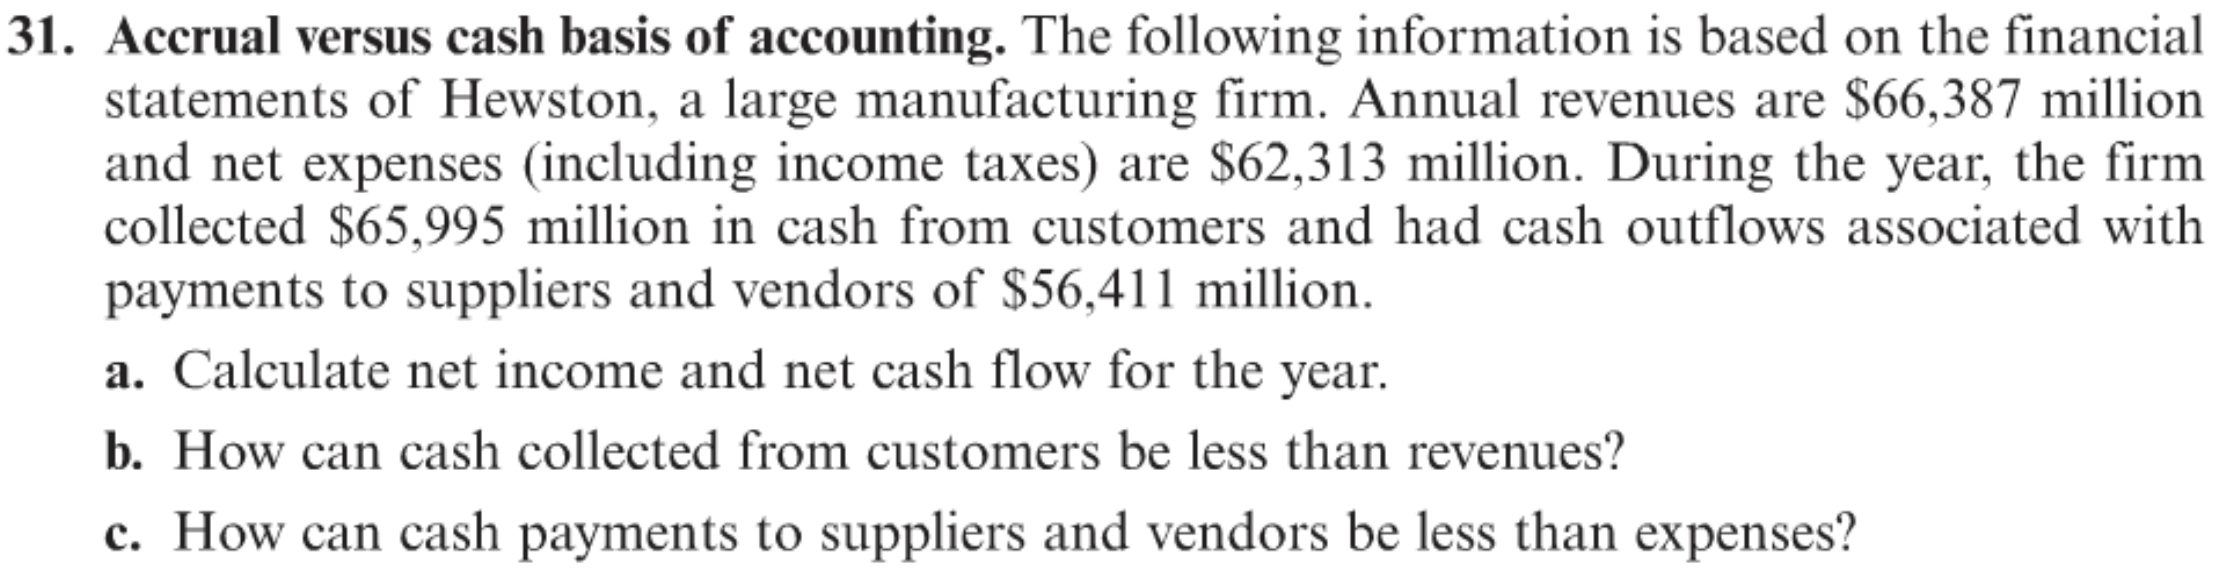
\includegraphics{images/재무회계_hw2_1-31.png}

}

\caption{Chapter1-31}

\end{figure}%

\subsection*{\texorpdfstring{\textbf{\emph{Answer}}}{Answer}}\label{answer-12}
\addcontentsline{toc}{subsection}{\textbf{\emph{Answer}}}

\textbf{\((a)\)} \(net\; income=66387-62313=4,074million\$\)

\(net\; cash\;flow=65995-56411=9,584million\$\)

\textbf{\((b)\)} If customer buy a product of Hewston and want to pay
later, then Hewston get a certain amount of revenue but get no cash.
Instead, Hewston get a asset, namely accrued revenue, that will be paid
for cash.

In that case, a company can get revenues more than collected cash.

\textbf{\((c)\)} If Hewston buy material from suppliers and vendors to
produce its own products but want to pay after selling product, then
there exists a certain amount of expense and occurs a liability, namely
accrued expense, that will pay for cash.

In that case, a company's expenses is bigger than its cash payments.

\section*{(2) Quetion 1-34}\label{quetion-1-34}
\addcontentsline{toc}{section}{(2) Quetion 1-34}

\markright{(2) Quetion 1-34}

\begin{figure}[H]

{\centering 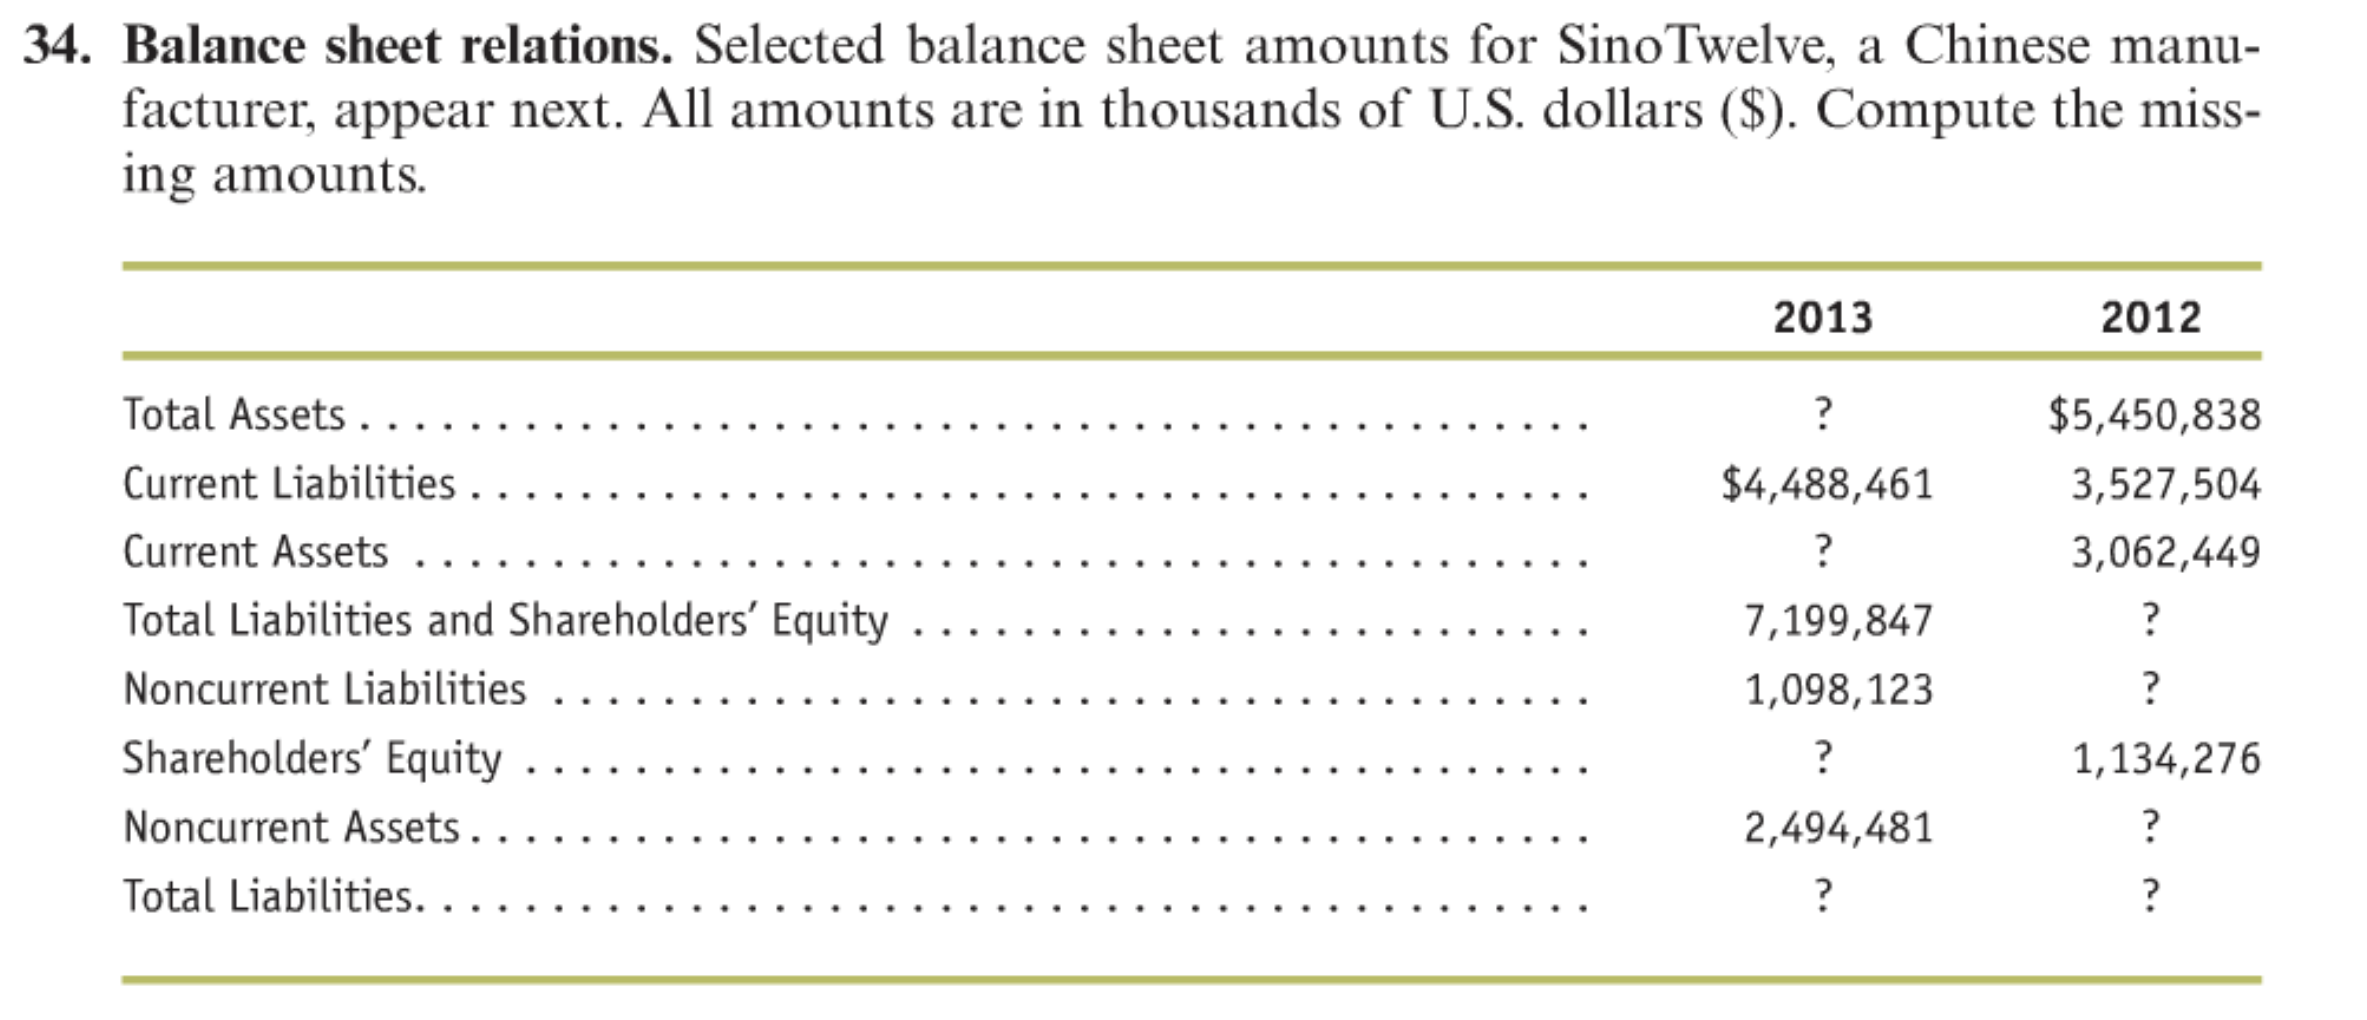
\includegraphics{images/재무회계_hw2_1-34.png}

}

\caption{Chapter1-34}

\end{figure}%

\subsection*{\texorpdfstring{\textbf{\emph{Answer}}}{Answer}}\label{answer-13}
\addcontentsline{toc}{subsection}{\textbf{\emph{Answer}}}

\emph{Total Assets = Current Assets + Noncurrent Assets}

\emph{Total Liabilities = Current Liabilities + Noncurrent Liabilities}

\emph{Total Liabilities and Shareholders' Equity = Total Liabilities +
Shareholders' Equity}

And, \emph{Total Assets = Total Liabilities and Shareholders' Equity}

Apply above,

\begin{longtable}[]{@{}
  >{\raggedright\arraybackslash}p{(\columnwidth - 4\tabcolsep) * \real{0.5915}}
  >{\raggedleft\arraybackslash}p{(\columnwidth - 4\tabcolsep) * \real{0.2113}}
  >{\raggedleft\arraybackslash}p{(\columnwidth - 4\tabcolsep) * \real{0.1972}}@{}}
\toprule\noalign{}
\begin{minipage}[b]{\linewidth}\raggedright
Category
\end{minipage} & \begin{minipage}[b]{\linewidth}\raggedleft
2013
\end{minipage} & \begin{minipage}[b]{\linewidth}\raggedleft
2012
\end{minipage} \\
\midrule\noalign{}
\endhead
\bottomrule\noalign{}
\endlastfoot
Total Assets & \textbf{7,199,847} & 5,450,838 \\
Current Liabilities & 4,488,461 & 3,527,504 \\
Current Assets & \textbf{4,705,366} & 3,062,449 \\
Total Liabilities and Shareholders' Equity & 7,199,847 &
\textbf{5,450,838} \\
Noncurrent Liabilities & 1,098,123 & 789,058 \\
Shareholders' Equity & \textbf{1,613,263} & 1,134,276 \\
Noncurrent Assets & 2,494,481 & 2,388,389 \\
Total Liabilities & \textbf{5,586,594} & \textbf{4,316,562} \\
\end{longtable}

\section*{(3) Quetion 2-10}\label{quetion-2-10}
\addcontentsline{toc}{section}{(3) Quetion 2-10}

\markright{(3) Quetion 2-10}

\begin{figure}[H]

{\centering 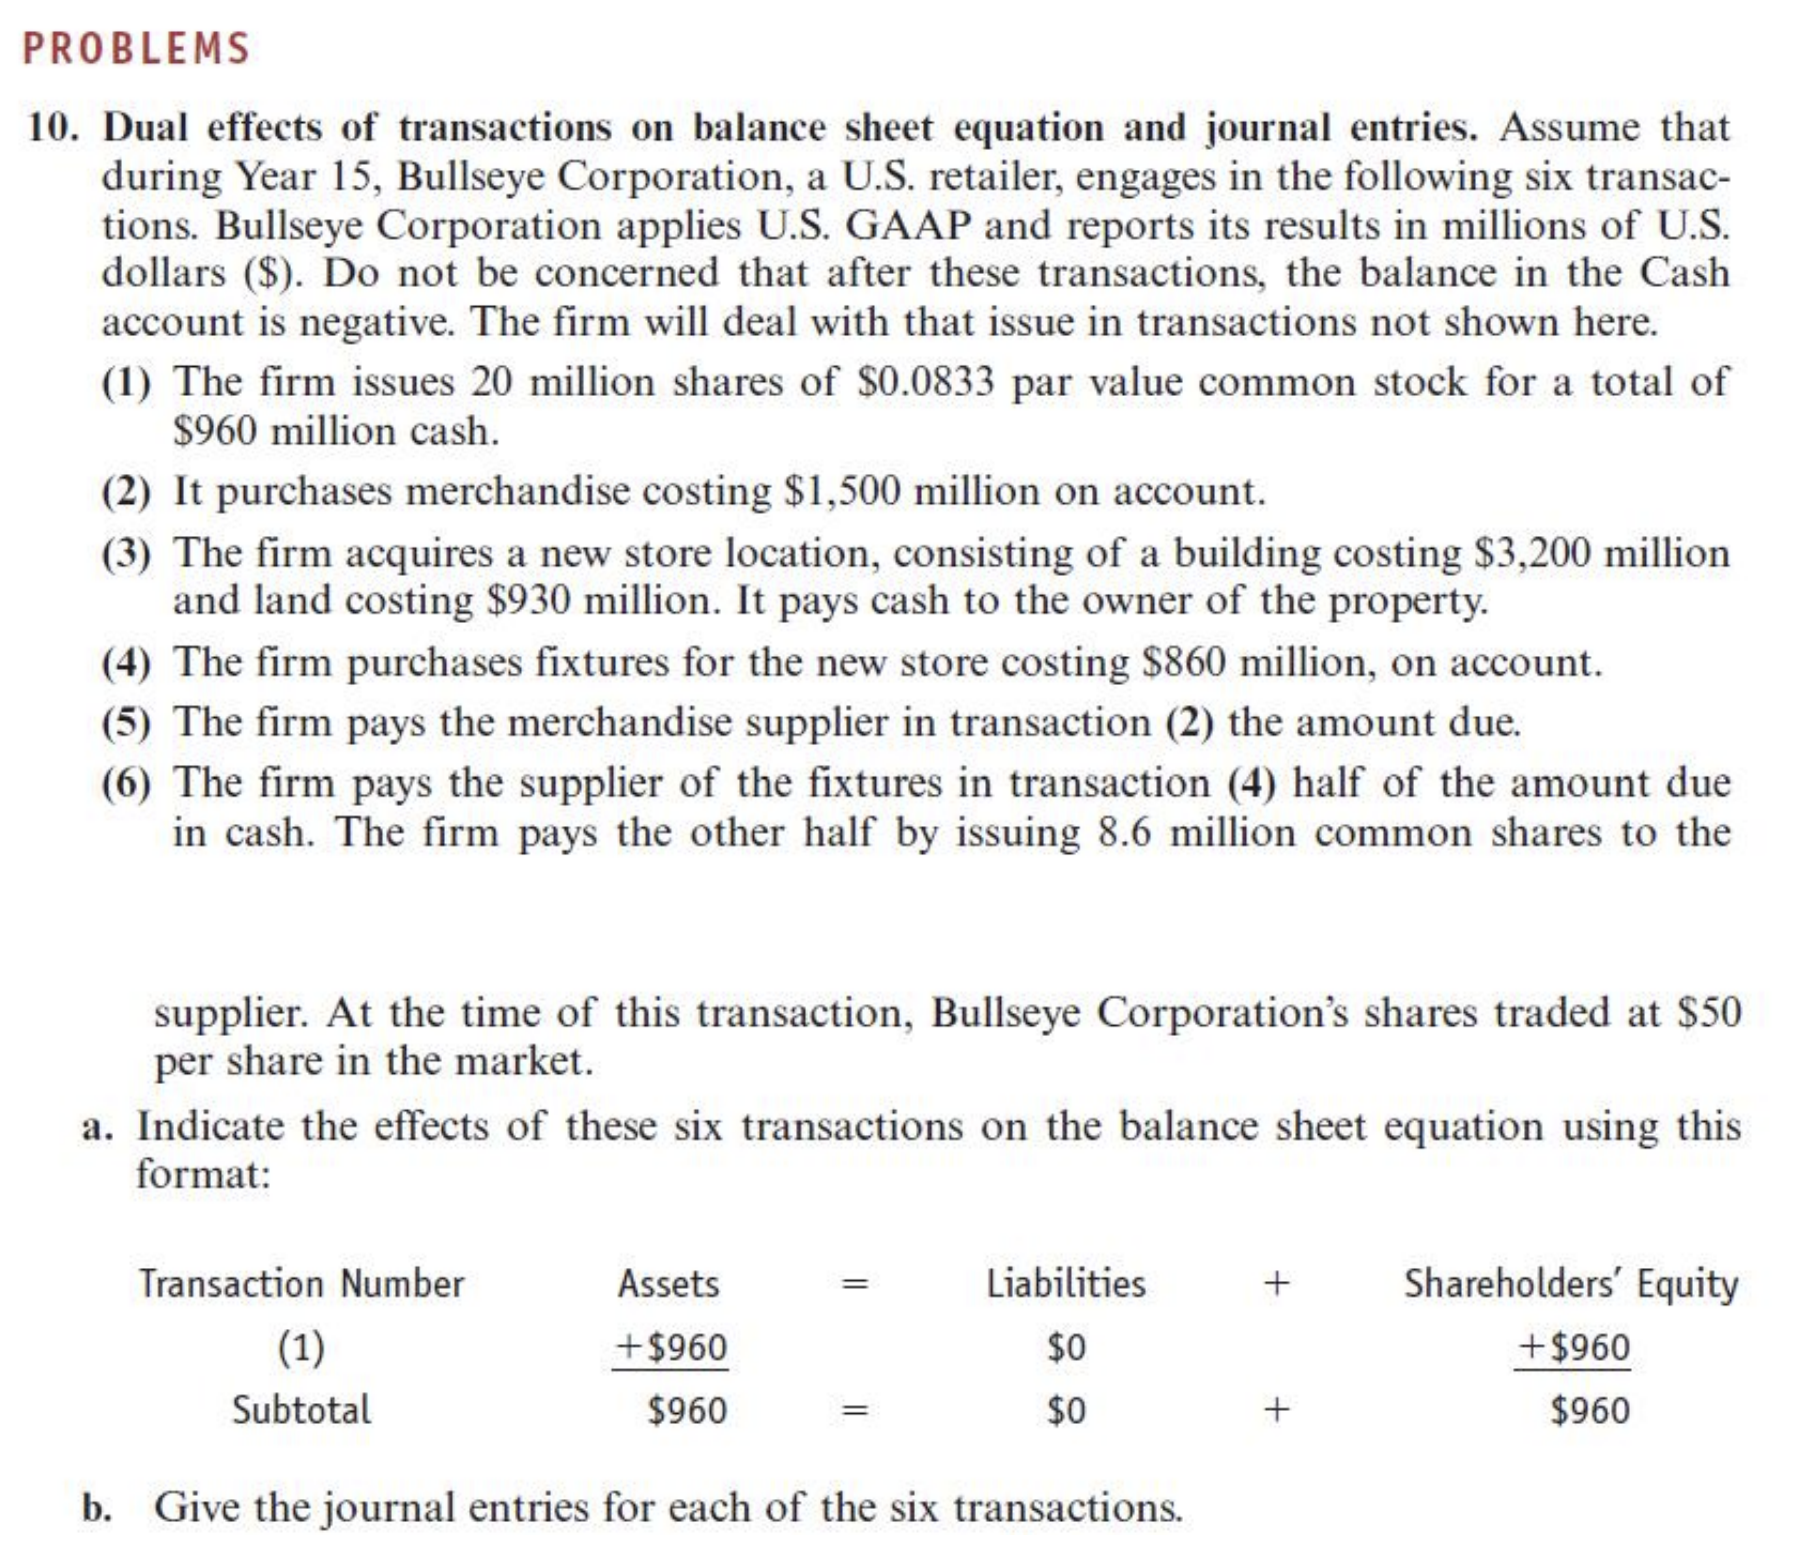
\includegraphics{images/재무회계_hw2_2-10.png}

}

\caption{Chapter2-10}

\end{figure}%

\subsection*{\texorpdfstring{\textbf{\emph{Answer}}}{Answer}}\label{answer-14}
\addcontentsline{toc}{subsection}{\textbf{\emph{Answer}}}

\textbf{\((a)\)}

\begin{longtable}[]{@{}
  >{\centering\arraybackslash}p{(\columnwidth - 10\tabcolsep) * \real{0.2985}}
  >{\raggedleft\arraybackslash}p{(\columnwidth - 10\tabcolsep) * \real{0.1493}}
  >{\raggedright\arraybackslash}p{(\columnwidth - 10\tabcolsep) * \real{0.0448}}
  >{\raggedleft\arraybackslash}p{(\columnwidth - 10\tabcolsep) * \real{0.1642}}
  >{\raggedright\arraybackslash}p{(\columnwidth - 10\tabcolsep) * \real{0.0448}}
  >{\raggedleft\arraybackslash}p{(\columnwidth - 10\tabcolsep) * \real{0.2985}}@{}}
\toprule\noalign{}
\begin{minipage}[b]{\linewidth}\centering
Transaction Number
\end{minipage} & \begin{minipage}[b]{\linewidth}\raggedleft
Assets
\end{minipage} & \begin{minipage}[b]{\linewidth}\raggedright
=
\end{minipage} & \begin{minipage}[b]{\linewidth}\raggedleft
Liabilities
\end{minipage} & \begin{minipage}[b]{\linewidth}\raggedright
+
\end{minipage} & \begin{minipage}[b]{\linewidth}\raggedleft
Shareholder's Equity
\end{minipage} \\
\midrule\noalign{}
\endhead
\bottomrule\noalign{}
\endlastfoot
(1) & +\$960m & & \$0 & & +\$960m \\
(2) & +\$1,500m & & +\$1,500m & & \$0 \\
(3) & +\$3,200m +\$930m -\$4,130m & & \$0 & & \$0 \\
(4) & +\$860m & & +\$860m & & \$0 \\
(5) & -\$1,500m & & -\$1,500m & & \$0 \\
(6) & -\$430m +\$430m -\$430m & & -\$430m -\$430m & & +\$430m \\
\textbf{Total} & \textbf{\$1,390m} & = & \textbf{\$0} & + &
\textbf{\$1,390m} \\
\end{longtable}

\textbf{\((b)\)}

\begin{longtable}[]{@{}lrr@{}}
\toprule\noalign{}
Transaction Num. (1) & Debit & Credit \\
\midrule\noalign{}
\endhead
\bottomrule\noalign{}
\endlastfoot
Cash & \$960m & \\
Common stock & & \$1.7m \\
Additional capital & & \$958.3m \\
\end{longtable}

\begin{longtable}[]{@{}lrr@{}}
\toprule\noalign{}
Transaction Num. (2) & Debit & Credit \\
\midrule\noalign{}
\endhead
\bottomrule\noalign{}
\endlastfoot
Inventory & \$1,500m & \\
Payable & & \$1,500m \\
\end{longtable}

\begin{longtable}[]{@{}lrr@{}}
\toprule\noalign{}
Transaction Num. (3) & Debit & Credit \\
\midrule\noalign{}
\endhead
\bottomrule\noalign{}
\endlastfoot
Building & \$3,200m & \\
Landscape & \$930m & \\
Cash paid & & \$4,130m \\
\end{longtable}

\begin{longtable}[]{@{}lrr@{}}
\toprule\noalign{}
Transaction Num. (4) & Debit & Credit \\
\midrule\noalign{}
\endhead
\bottomrule\noalign{}
\endlastfoot
Fixture & \$860m & \\
Payable & & \$860m \\
\end{longtable}

\begin{longtable}[]{@{}lrr@{}}
\toprule\noalign{}
Transaction Num. (5) & Debit & Credit \\
\midrule\noalign{}
\endhead
\bottomrule\noalign{}
\endlastfoot
Payable & \$1,500m & \\
Cash & & \$1,500m \\
\end{longtable}

\begin{longtable}[]{@{}lrr@{}}
\toprule\noalign{}
Transaction Num. (6) & Debit & Credit \\
\midrule\noalign{}
\endhead
\bottomrule\noalign{}
\endlastfoot
Payable & \$430m & \\
Cash paid & & \$430m \\
Cash & \$430m & \\
Common stock & & \$0.7m \\
Additional capital & & \$429.3m \\
Payable & \$430m & \\
Cash paid & & \$430m \\
\end{longtable}

\section*{(4) Quetion 3-12}\label{quetion-3-12}
\addcontentsline{toc}{section}{(4) Quetion 3-12}

\markright{(4) Quetion 3-12}

\begin{figure}[H]

{\centering 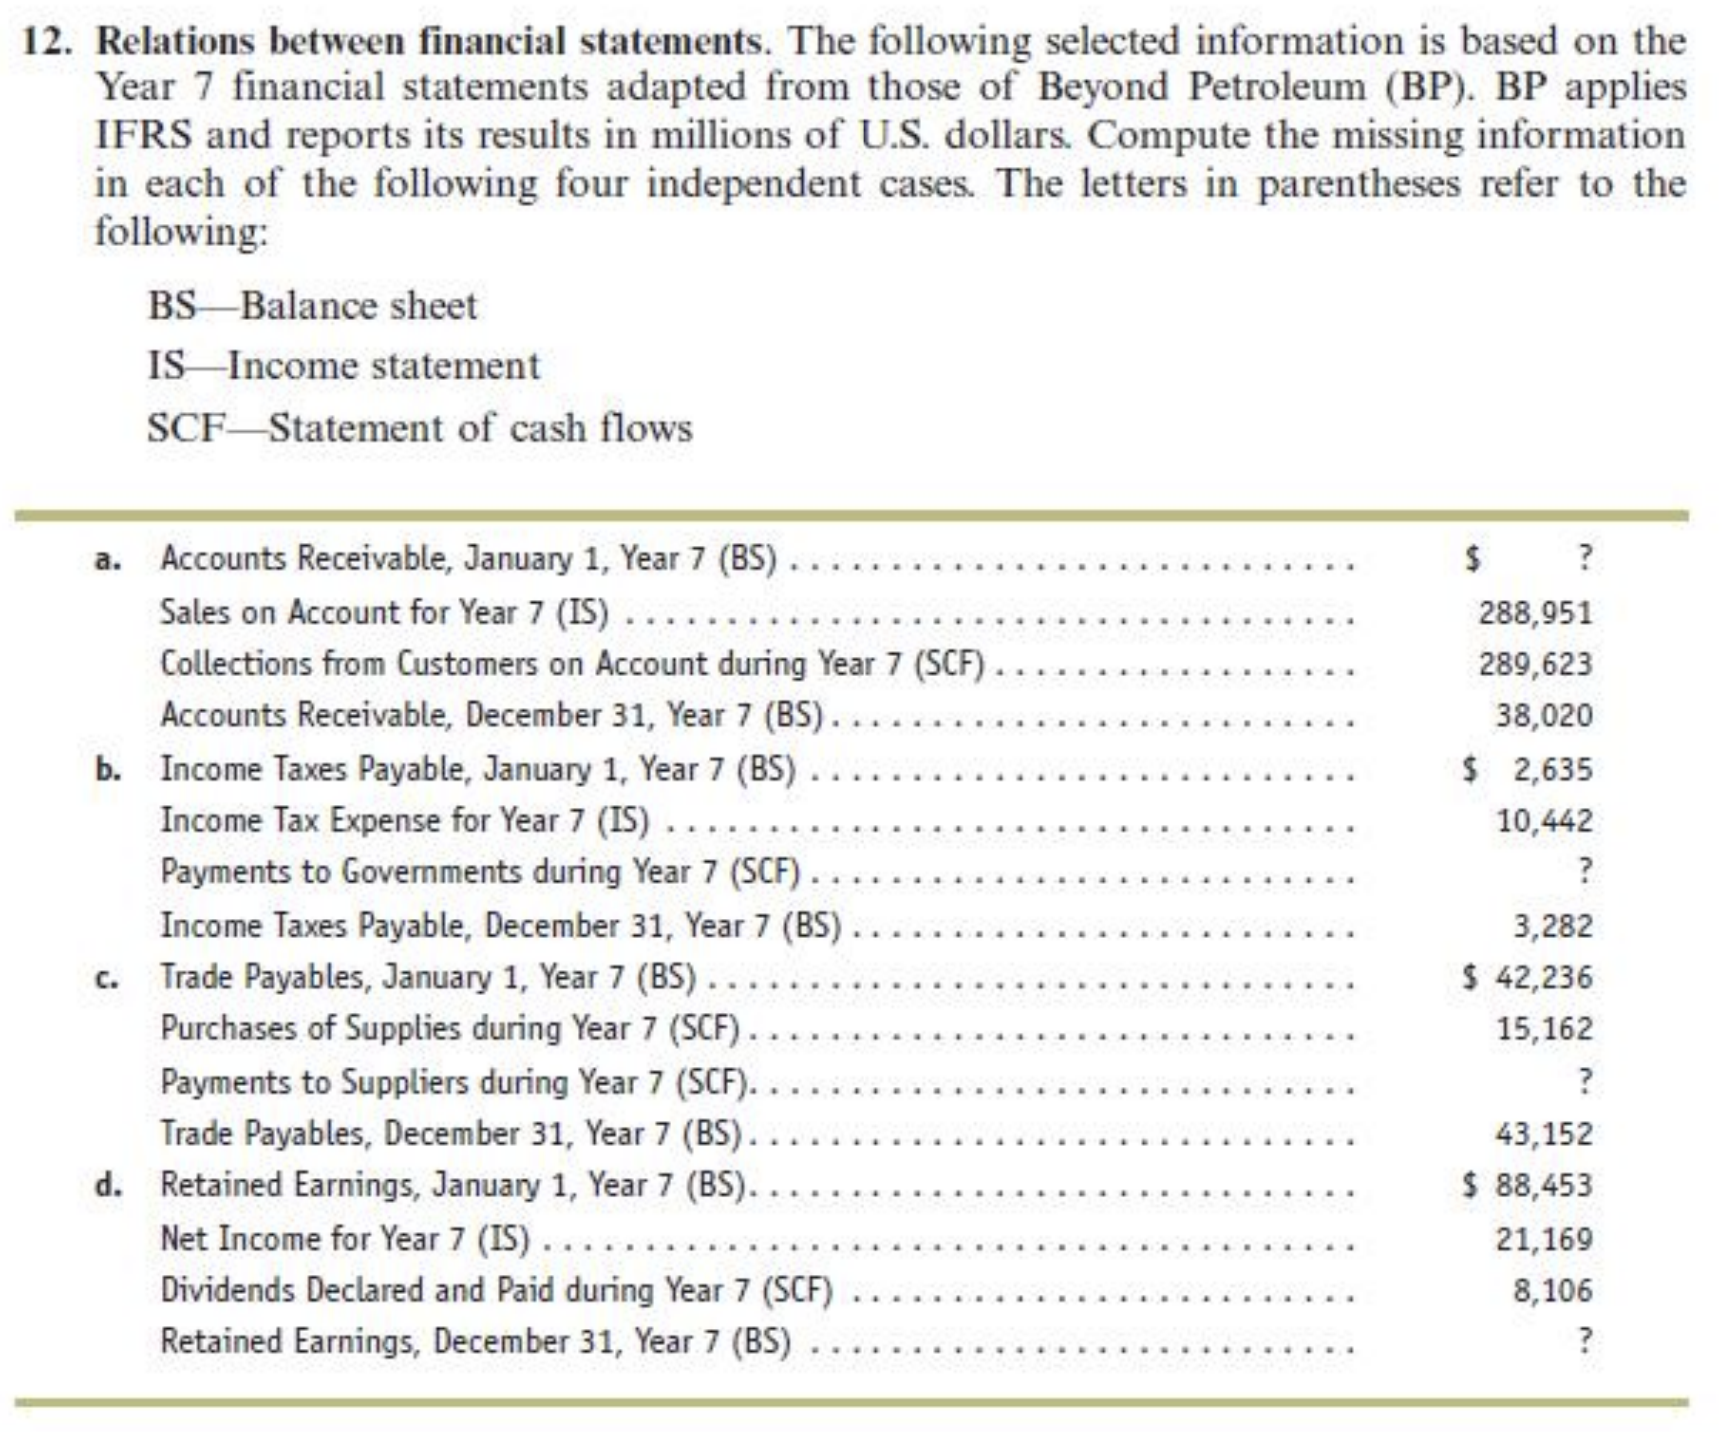
\includegraphics{images/재무회계_hw2_3-12.png}

}

\caption{Chapter3-10}

\end{figure}%

\subsection*{\texorpdfstring{\textbf{\emph{Answer}}}{Answer}}\label{answer-15}
\addcontentsline{toc}{subsection}{\textbf{\emph{Answer}}}

\textbf{\((a)\)}

\[Accounts\,Receivable\,in\,Jan.+288,951-289,623=38,020\]

\[Accounts\,Receivable\,in\,Jan.=\$38,692\]

\textbf{\((b)\)} \[2,635+10,442-Payments\,to\,Gov.=3,282\]

\[Payments\,to\,Gov.=\$9,795\]

\textbf{\((c)\)}

\[42,236+15,162-Payments\,to\,suppliers=43,152\]

\[Payments\,to\,suppliers=\$14,246\]

\textbf{\((d)\)}

\[88,453+21,169-8,106=Retained\,Earnings\,in\,Dec.\]

\[Retained\,Earnings\,in\,Dec.=\$101,516\]

\chapter*{재무회계 Ch4
과제}\label{uxc7acuxbb34uxd68cuxacc4-ch4-uxacfcuxc81c}
\addcontentsline{toc}{chapter}{재무회계 Ch4 과제}

\markboth{재무회계 Ch4 과제}{재무회계 Ch4 과제}

\section*{(1) Quetion 4-9}\label{quetion-4-9}
\addcontentsline{toc}{section}{(1) Quetion 4-9}

\markright{(1) Quetion 4-9}

\begin{figure}[H]

{\centering 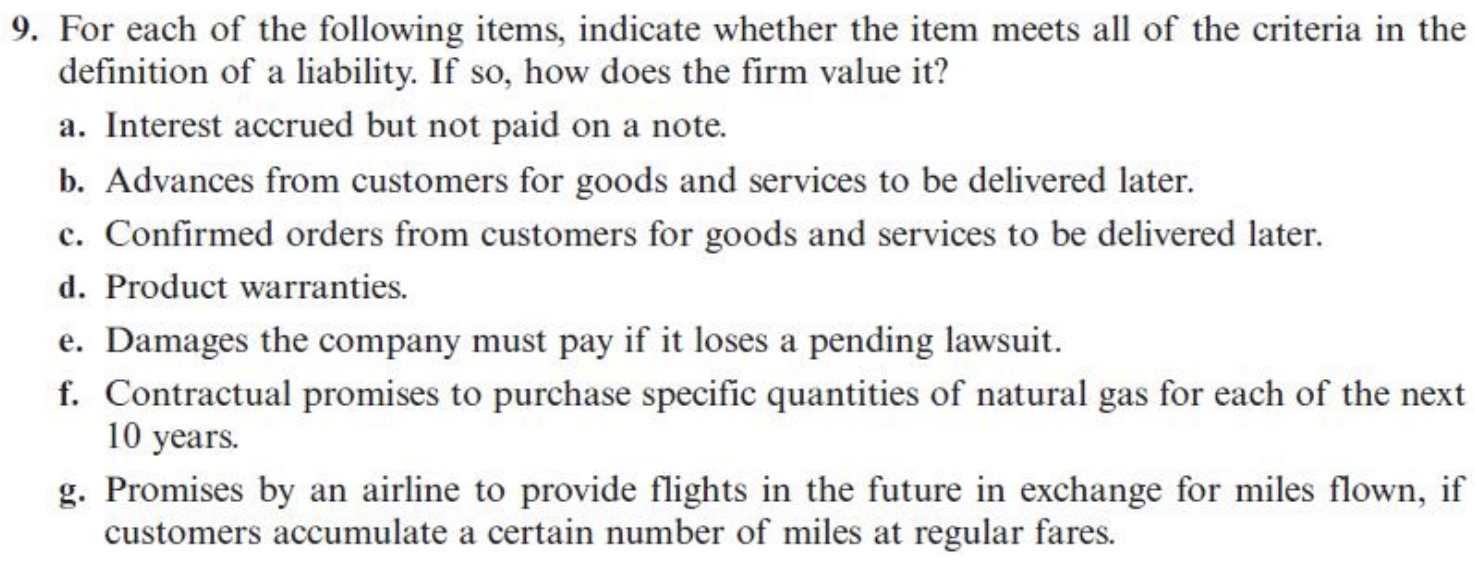
\includegraphics{images/재무회계_4-9.png}

}

\caption{Chapter4-9}

\end{figure}%

First, the criteria in the definition of a liablilty is following :

\begin{enumerate}
\def\labelenumi{(\arabic{enumi})}
\tightlist
\item
  Probably, future sacrifices of economic benefits.
\item
  Arising from present obligation to transfer assets of privide
  services.
\item
  As a result of a past transaction.
\end{enumerate}

In this perspective,

\textbf{(a) is a liability.} accrued interest payable.

\textbf{(b) is a liability.}(Advances from customers) It is equal to
amount of received cash.

\textbf{(c) is not a liability.} criteria (3) is not satisfied.

\textbf{(d) is a liability.}(Provisions) It can be valued by some ratio
of original product's price.

\textbf{(e) can be liability or not.} It depends on a probability of
lawsuit.

If a probability of loss lawsuit is more than certain level,(In GAAP
80\%, IFRS 50\%) then it will be a liability. In that case, it can be
valued by expected loss that should pay.

\textbf{(f) is not a liability.} criteria (3) is not satisfied.

\textbf{(g) is a liability.} It can be valued by some ratio of flight
ticket's regular price.

\section*{(2) Quetion 4-15}\label{quetion-4-15}
\addcontentsline{toc}{section}{(2) Quetion 4-15}

\markright{(2) Quetion 4-15}

\begin{figure}[H]

{\centering 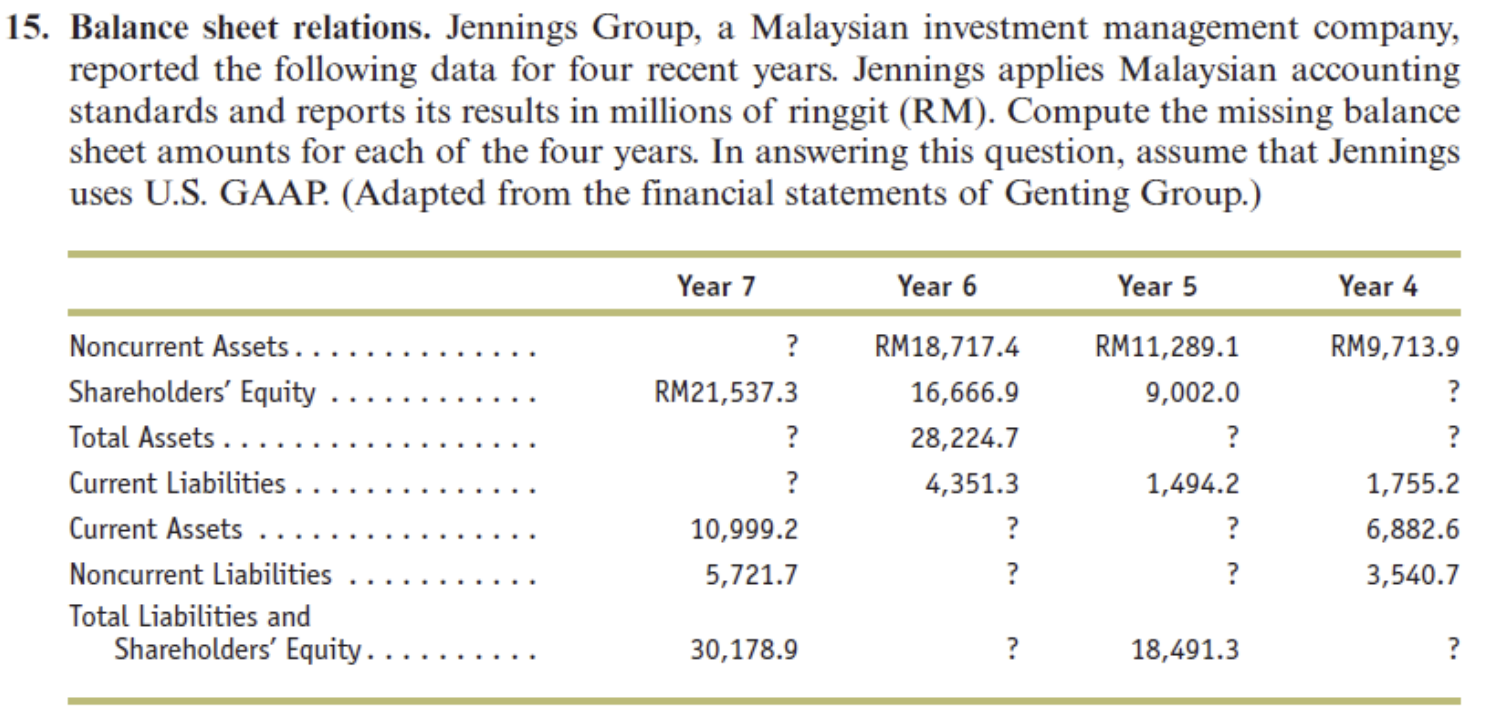
\includegraphics{images/재무회계_4-15.png}

}

\caption{Chapter4-15}

\end{figure}%

\emph{Total Assets = Current Assets + Noncurrent Assets}

\emph{Total Liabilities = Current Liabilities + Noncurrent Liabilities}

\emph{Total Liabilities and Shareholders' Equity = Total Liabilities +
Shareholders' Equity}

And, \emph{Total Assets = Total Liabilities and Shareholders' Equity}

Apply above,

\begin{longtable}[]{@{}
  >{\raggedright\arraybackslash}p{(\columnwidth - 8\tabcolsep) * \real{0.4512}}
  >{\raggedleft\arraybackslash}p{(\columnwidth - 8\tabcolsep) * \real{0.1463}}
  >{\raggedleft\arraybackslash}p{(\columnwidth - 8\tabcolsep) * \real{0.1341}}
  >{\raggedleft\arraybackslash}p{(\columnwidth - 8\tabcolsep) * \real{0.1341}}
  >{\raggedleft\arraybackslash}p{(\columnwidth - 8\tabcolsep) * \real{0.1341}}@{}}
\toprule\noalign{}
\begin{minipage}[b]{\linewidth}\raggedright
Category
\end{minipage} & \begin{minipage}[b]{\linewidth}\raggedleft
Year7
\end{minipage} & \begin{minipage}[b]{\linewidth}\raggedleft
Year6
\end{minipage} & \begin{minipage}[b]{\linewidth}\raggedleft
Year5
\end{minipage} & \begin{minipage}[b]{\linewidth}\raggedleft
Year4
\end{minipage} \\
\midrule\noalign{}
\endhead
\bottomrule\noalign{}
\endlastfoot
Noncurrent Assets & \textbf{19,179.7} & 18,717.4 & 11,289.1 & 9,713.9 \\
Shareholders' Equity & 21,537.3 & 16,666.9 & 9,002.0 &
\textbf{11,300.6} \\
Total Assets & \textbf{30,178.9} & 28,224.7 & \textbf{18,491.3} &
\textbf{16,596.5} \\
Current Liabilities & \textbf{2,919.9} & 4,351.3 & 1,494.2 & 1,755.2 \\
Current Assets & 10,999.2 & \textbf{9,507.3} & \textbf{7,202.2} &
6,882.6 \\
Noncurrent Liabilities & 5,721.7 & \textbf{7,206.5} & \textbf{7,995.1} &
3,540.7 \\
Total Liabilities and Equity & 30,178.9 & \textbf{28,224.7} & 18,491.3 &
\textbf{16,596.5} \\
\end{longtable}

\chapter*{재무회계 Ch5
과제}\label{uxc7acuxbb34uxd68cuxacc4-ch5-uxacfcuxc81c}
\addcontentsline{toc}{chapter}{재무회계 Ch5 과제}

\markboth{재무회계 Ch5 과제}{재무회계 Ch5 과제}

\section*{(1) Question 5-12}\label{question-5-12}
\addcontentsline{toc}{section}{(1) Question 5-12}

\markright{(1) Question 5-12}

\begin{figure}[H]

{\centering 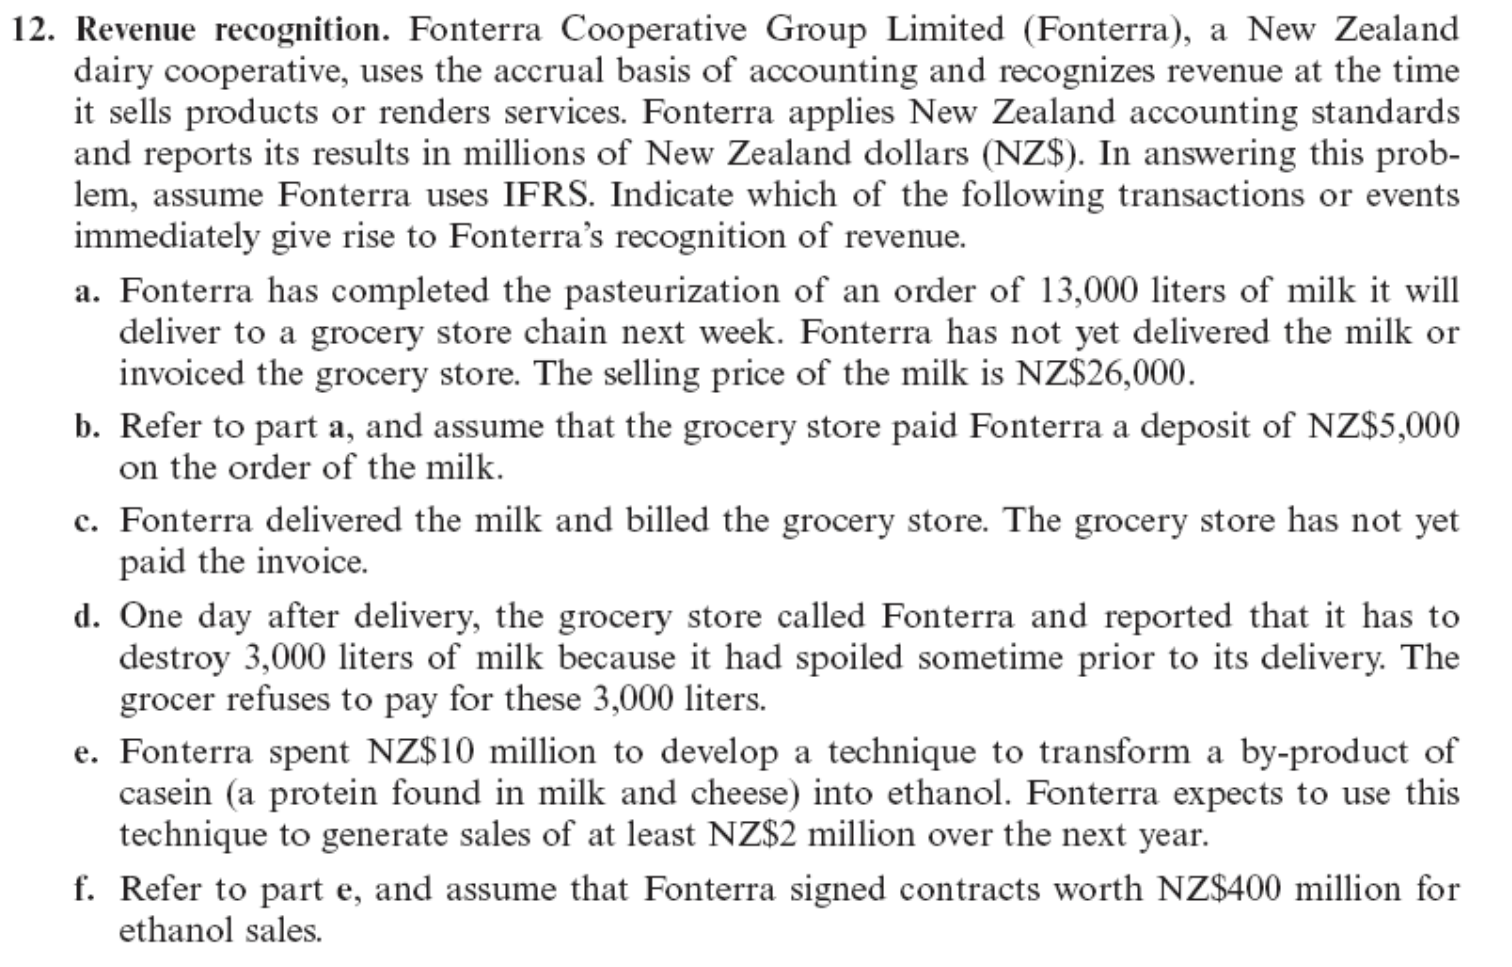
\includegraphics{images/재무회계_5-12.png}

}

\caption{Chapter5-12}

\end{figure}%

\begin{enumerate}
\def\labelenumi{(\alph{enumi})}
\tightlist
\item
  NOT recognized. It is before a completion of the earning process.
\item
  NOT recognized. It is before a completion of the earning process.
\item
  \textbf{Revenue recoginzed.} There is a completion of the earning
  process and receipt.(account receivable)
\item
  NOT recognized. It can be an expense.
\item
  NOT recognized. It is an investment, which is an expense.
\item
  NOT recognized. There is no completion of the earning process.
\end{enumerate}

\section*{(2) Question 5-18}\label{question-5-18}
\addcontentsline{toc}{section}{(2) Question 5-18}

\markright{(2) Question 5-18}

\begin{figure}[H]

{\centering 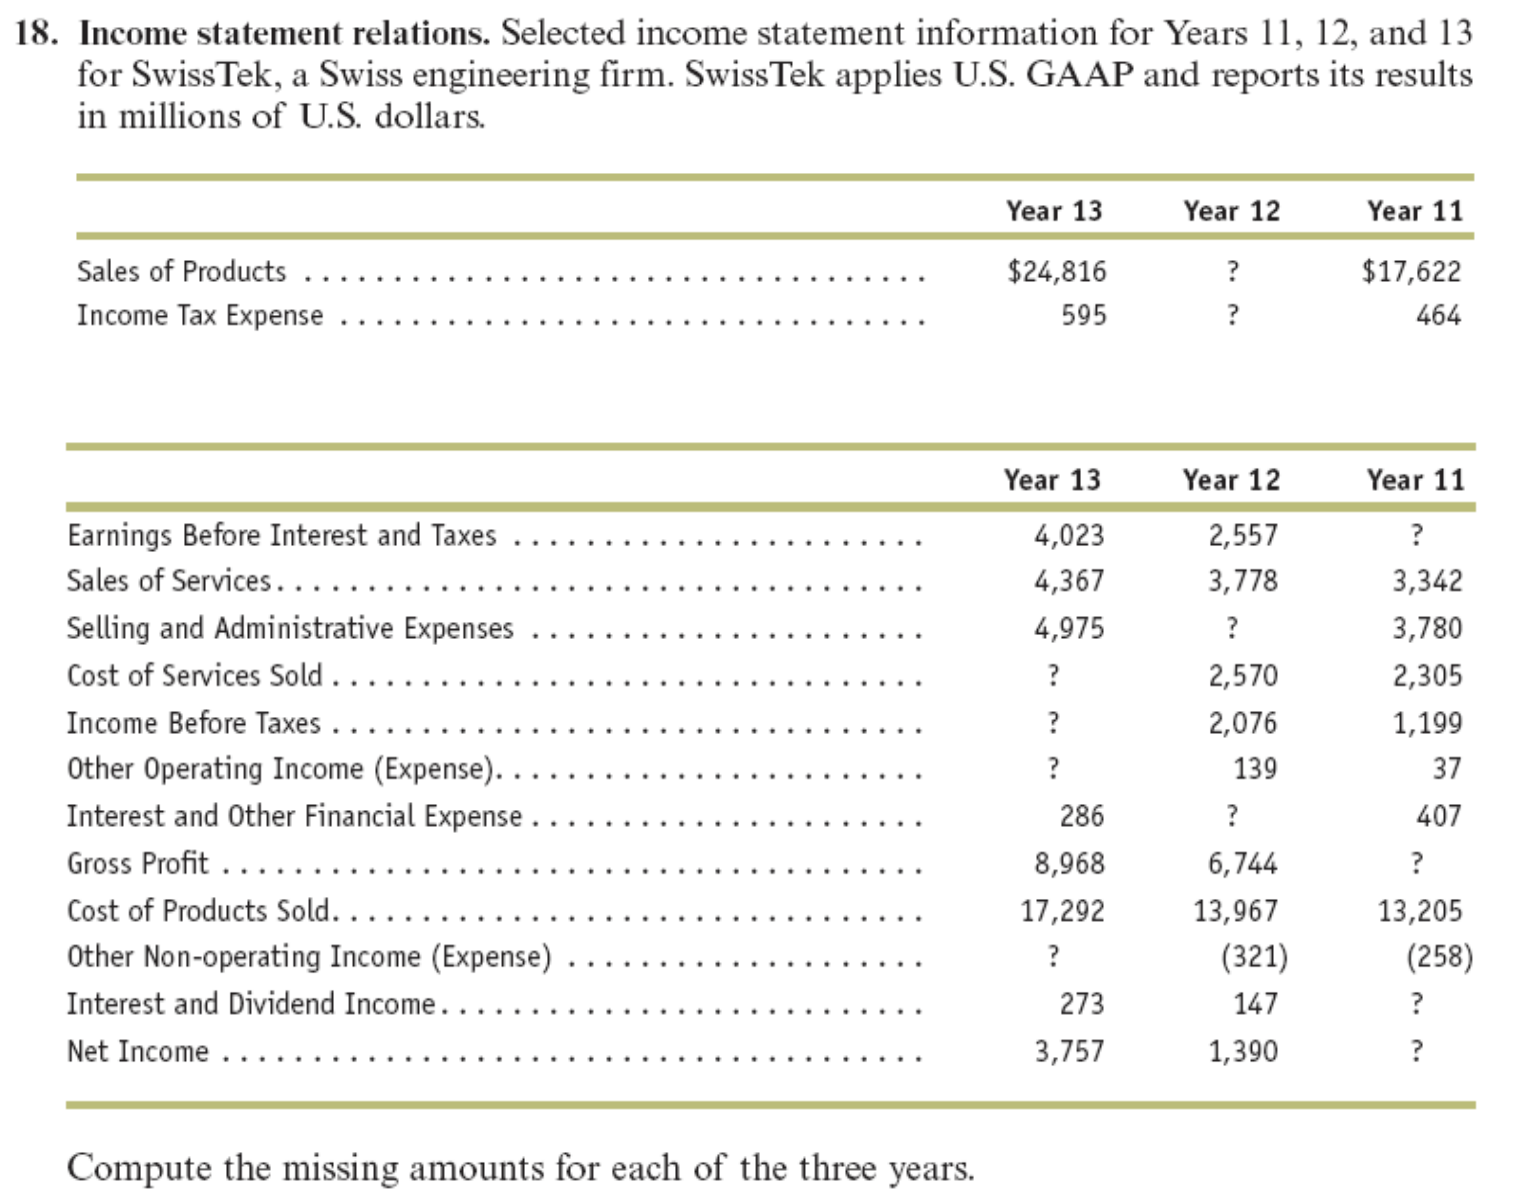
\includegraphics{images/재무회계_5-18.png}

}

\caption{Chapter5-18}

\end{figure}%

The following table is the re-organized income statement.

\begin{longtable}[]{@{}lrrr@{}}
\toprule\noalign{}
Category & Year 13 & Year 12 & Year 11 \\
\midrule\noalign{}
\endhead
\bottomrule\noalign{}
\endlastfoot
~(+) Sales of Products & 24,816 & \textbf{19,503} & 17,622 \\
~(-) Cost of Products Sold & 17,292 & 13,967 & 13,205 \\
~(+) Sales of Service & 4,367 & 3,778 & 3,342 \\
~(-) Cost of Services Sold & \textbf{2,923} & 2,570 & 2,305 \\
(=) \textbf{Gross Profit} & 8,968 & 6,744 & \textbf{5,454} \\
~(-) Selling and Administrative Expenses & 4,975 & \textbf{4,326} &
3,780 \\
~(+) Other Operating Income & \textbf{(30)} & 139 & 37 \\
(=) \textbf{Earning Before Interest and Taxes} & 4,023 & 2,557 &
\textbf{1,711} \\
~(+) Other Non-operating Income & \textbf{342} & (321) & (258) \\
~(+) Interest and Dividend Income & 273 & 147 & \textbf{153} \\
~(-) Interest and Other Financial Expense & 286 & \textbf{307} & 407 \\
(=) \textbf{Income Before Taxes} & \textbf{4,352} & 2,076 & 1,199 \\
~(-) Income Tax Expense & 595 & 686 & 464 \\
(=) \textbf{Net Income} & 3,757 & 1,390 & \textbf{735} \\
\end{longtable}

\chapter*{재무회계 Ch6
과제}\label{uxc7acuxbb34uxd68cuxacc4-ch6-uxacfcuxc81c}
\addcontentsline{toc}{chapter}{재무회계 Ch6 과제}

\markboth{재무회계 Ch6 과제}{재무회계 Ch6 과제}

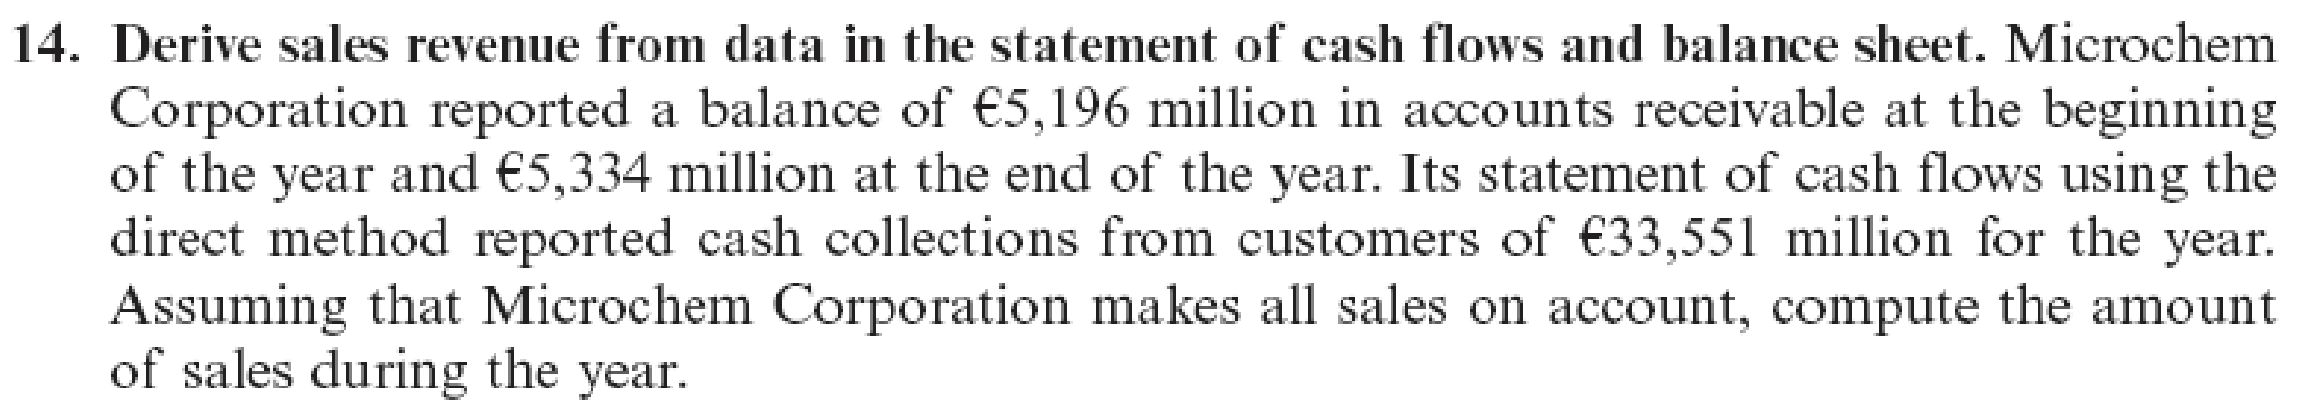
\includegraphics{images/재무회계_6-14.png}

\textbf{\emph{Answer}}

Because a company makes all sales on account, \textbf{total sales is sum
of cash collections and account receivable.}

There are EUR33,551m cash collections and EUR138m increase in account
receivavle, so 33551+138=\textbf{EUR33,689m will be a total sales} of
company during the year.

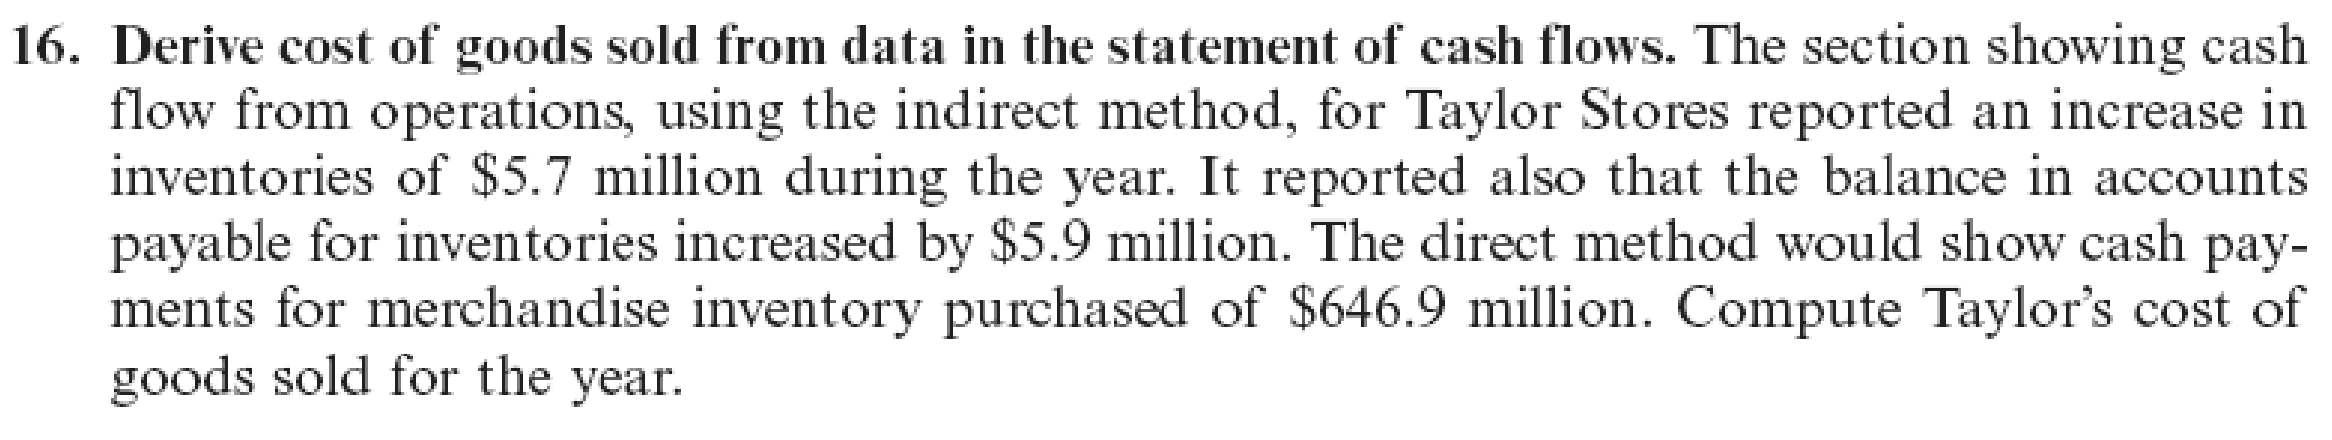
\includegraphics{images/재무회계_6-16.png}

\textbf{\emph{Answer}}

Cost will be \textbf{cash payments + increase payable - increase
inventories}.

646.9+5.9-5.7=\textbf{USD647.1m is cost of goods sold} of company for
the year.

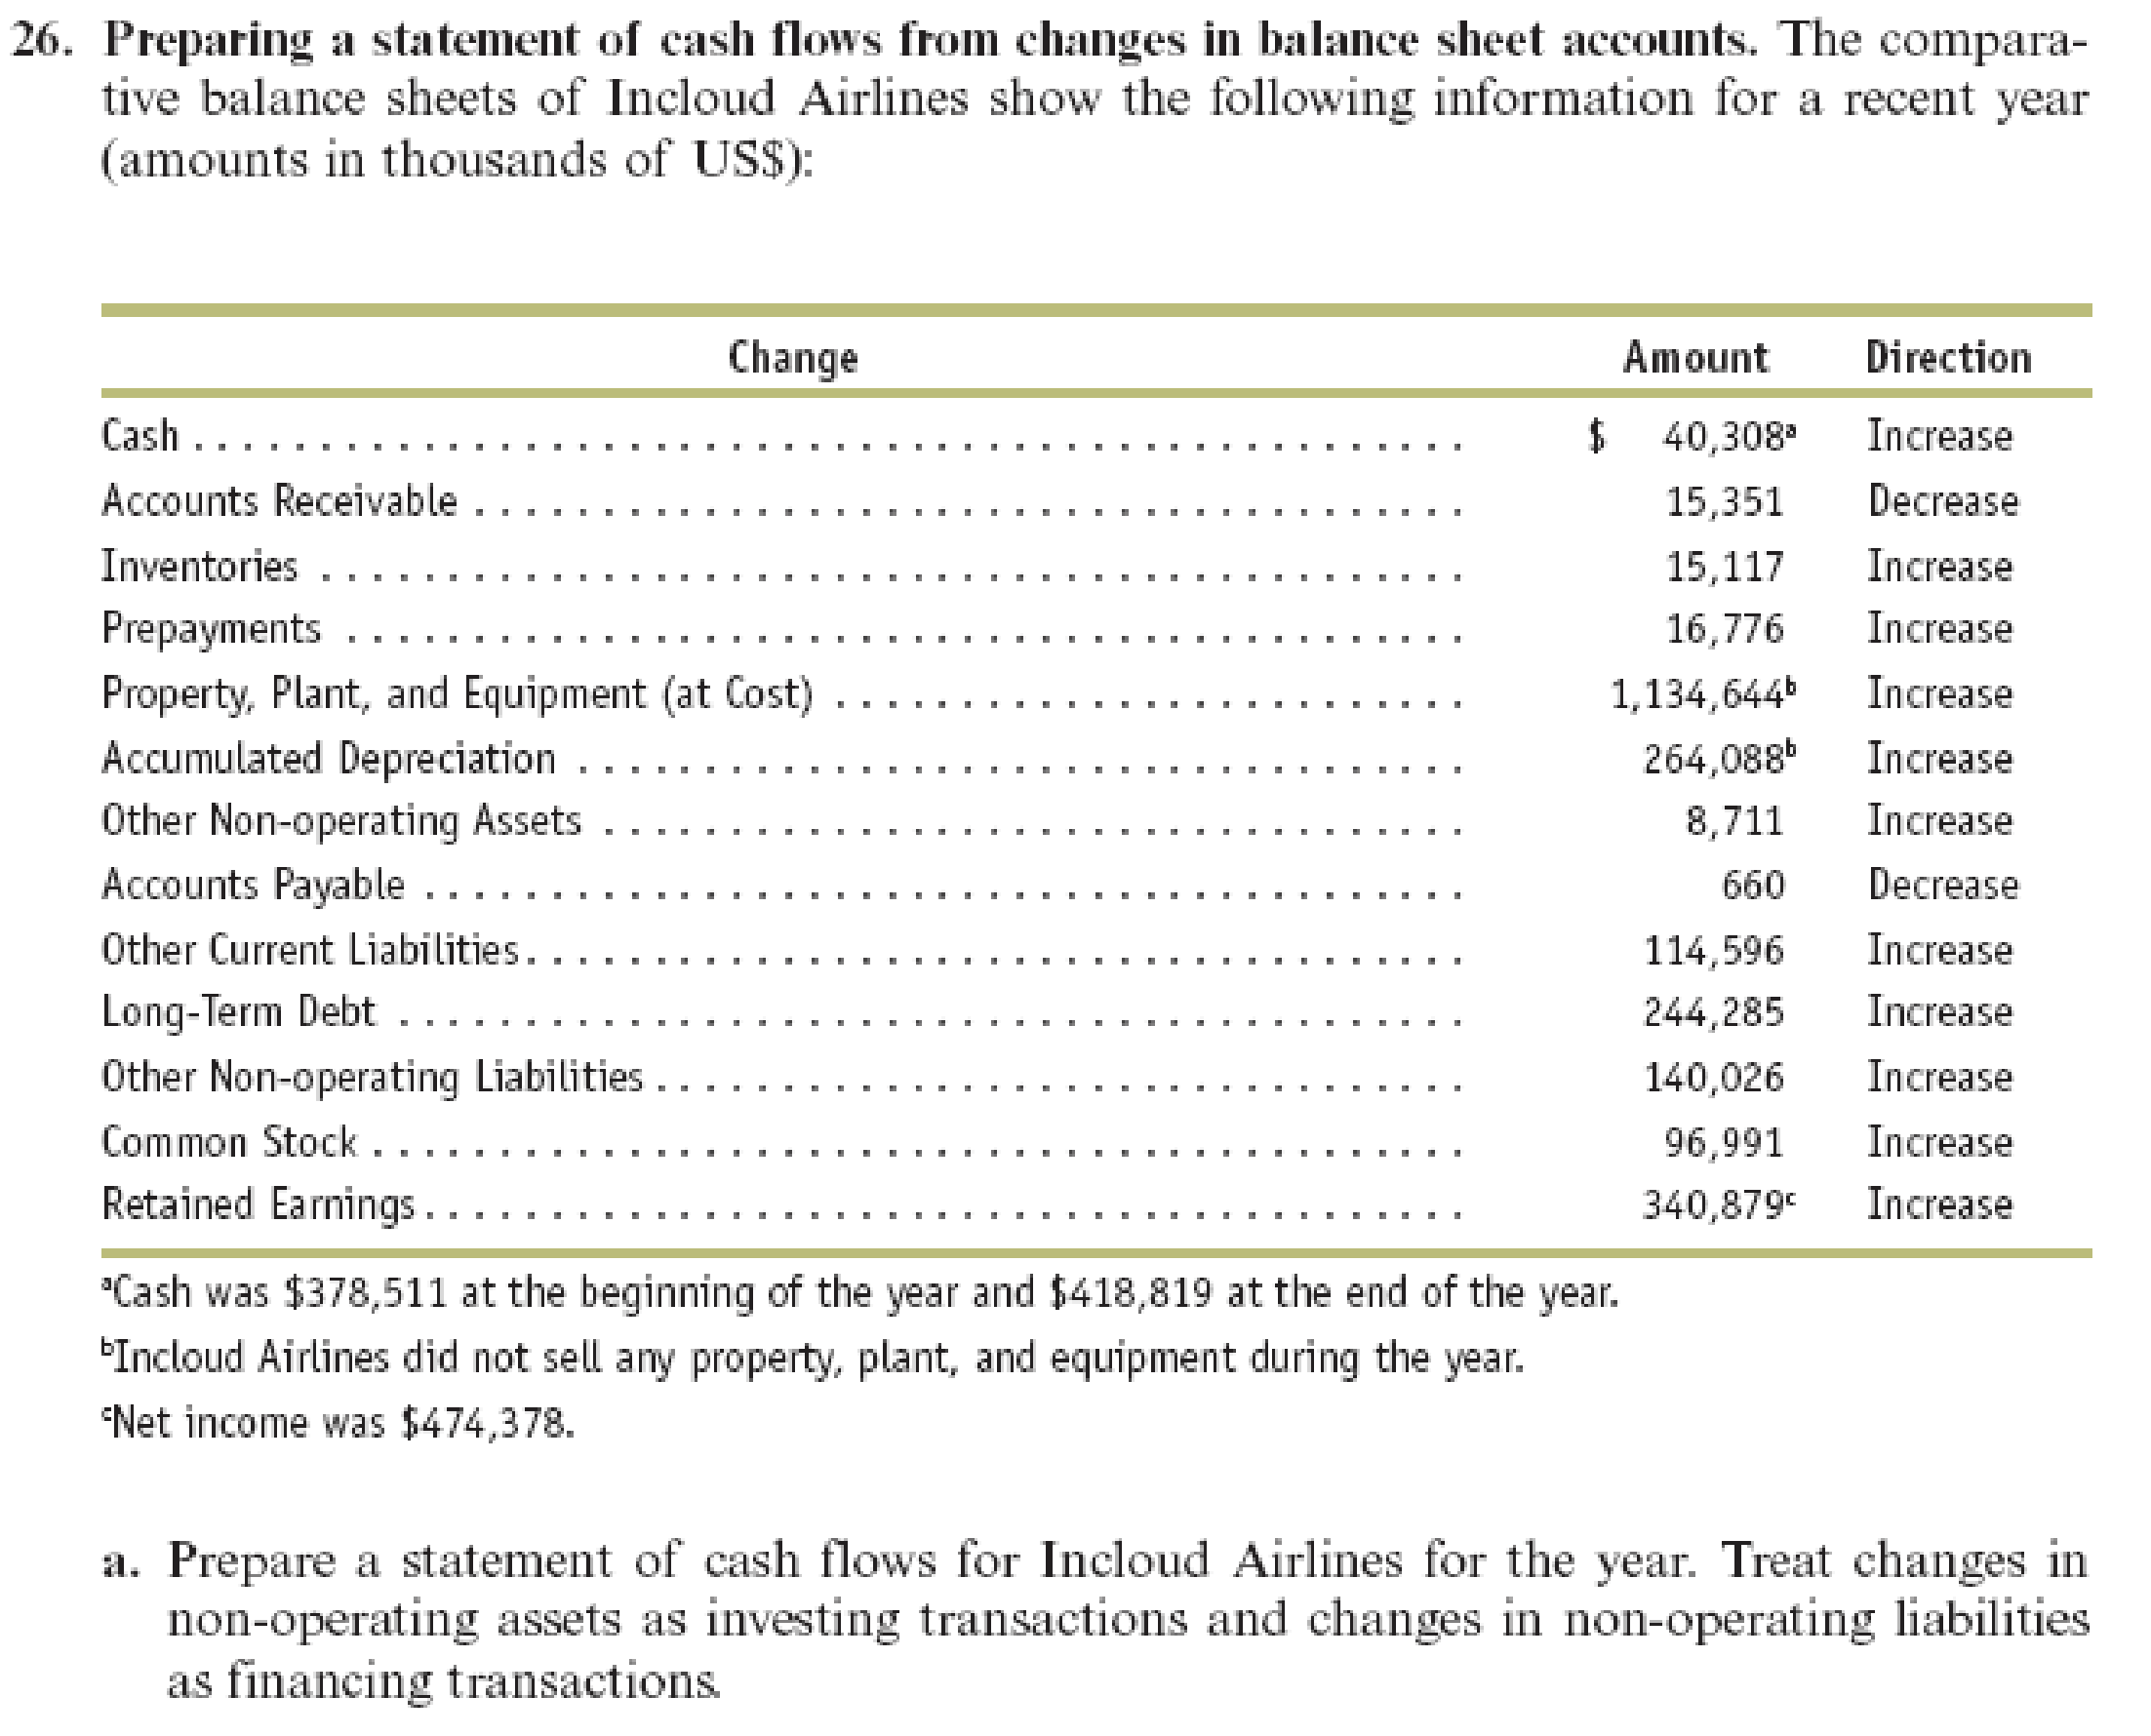
\includegraphics{images/재무회계_6-26.png}

\textbf{\emph{Answer}}

\[Incloud\;Airlines\]
\[Statement\;of\;Cash\;Flow\;for\;the\;recent\;year(thousands\$)\]

\begin{longtable}[]{@{}clr@{}}
\toprule\noalign{}
Category & Name & Amount \\
\midrule\noalign{}
\endhead
\bottomrule\noalign{}
\endlastfoot
Cashflow from operations & & \textbf{\$835,860} \\
+ & Net income & 474378 \\
+ & Increase in accumulated depreciation & 264088 \\
+ & Decrease in account receivable & 15351 \\
- & Increase in other current liabilities & 114596 \\
- & Increase in inventories & 15117 \\
- & Increase in Prepayments & 16776 \\
- & Decrease in account payable & 660 \\
Cashflow from investing & & \textbf{(\$1,143,355)} \\
- & Increase in property, plant, equipment & 1134644 \\
- & Increasing in other non-operating assets & 8711 \\
Cashflow from financing & & \textbf{\$347,803} \\
+ & Increasing in long-term debt & 244285 \\
+ & Increasing in common stock & 96991 \\
+ & Increasing in non-operating liabilities & 140026 \\
- & Payment of dividends & 133499 \\
\textbf{Net Change in Cash} & & \textbf{\$40,308} \\
Cash, beginning of year & & \textbf{\$378,511} \\
Cash, end of year & & \textbf{\$418,819} \\
\end{longtable}

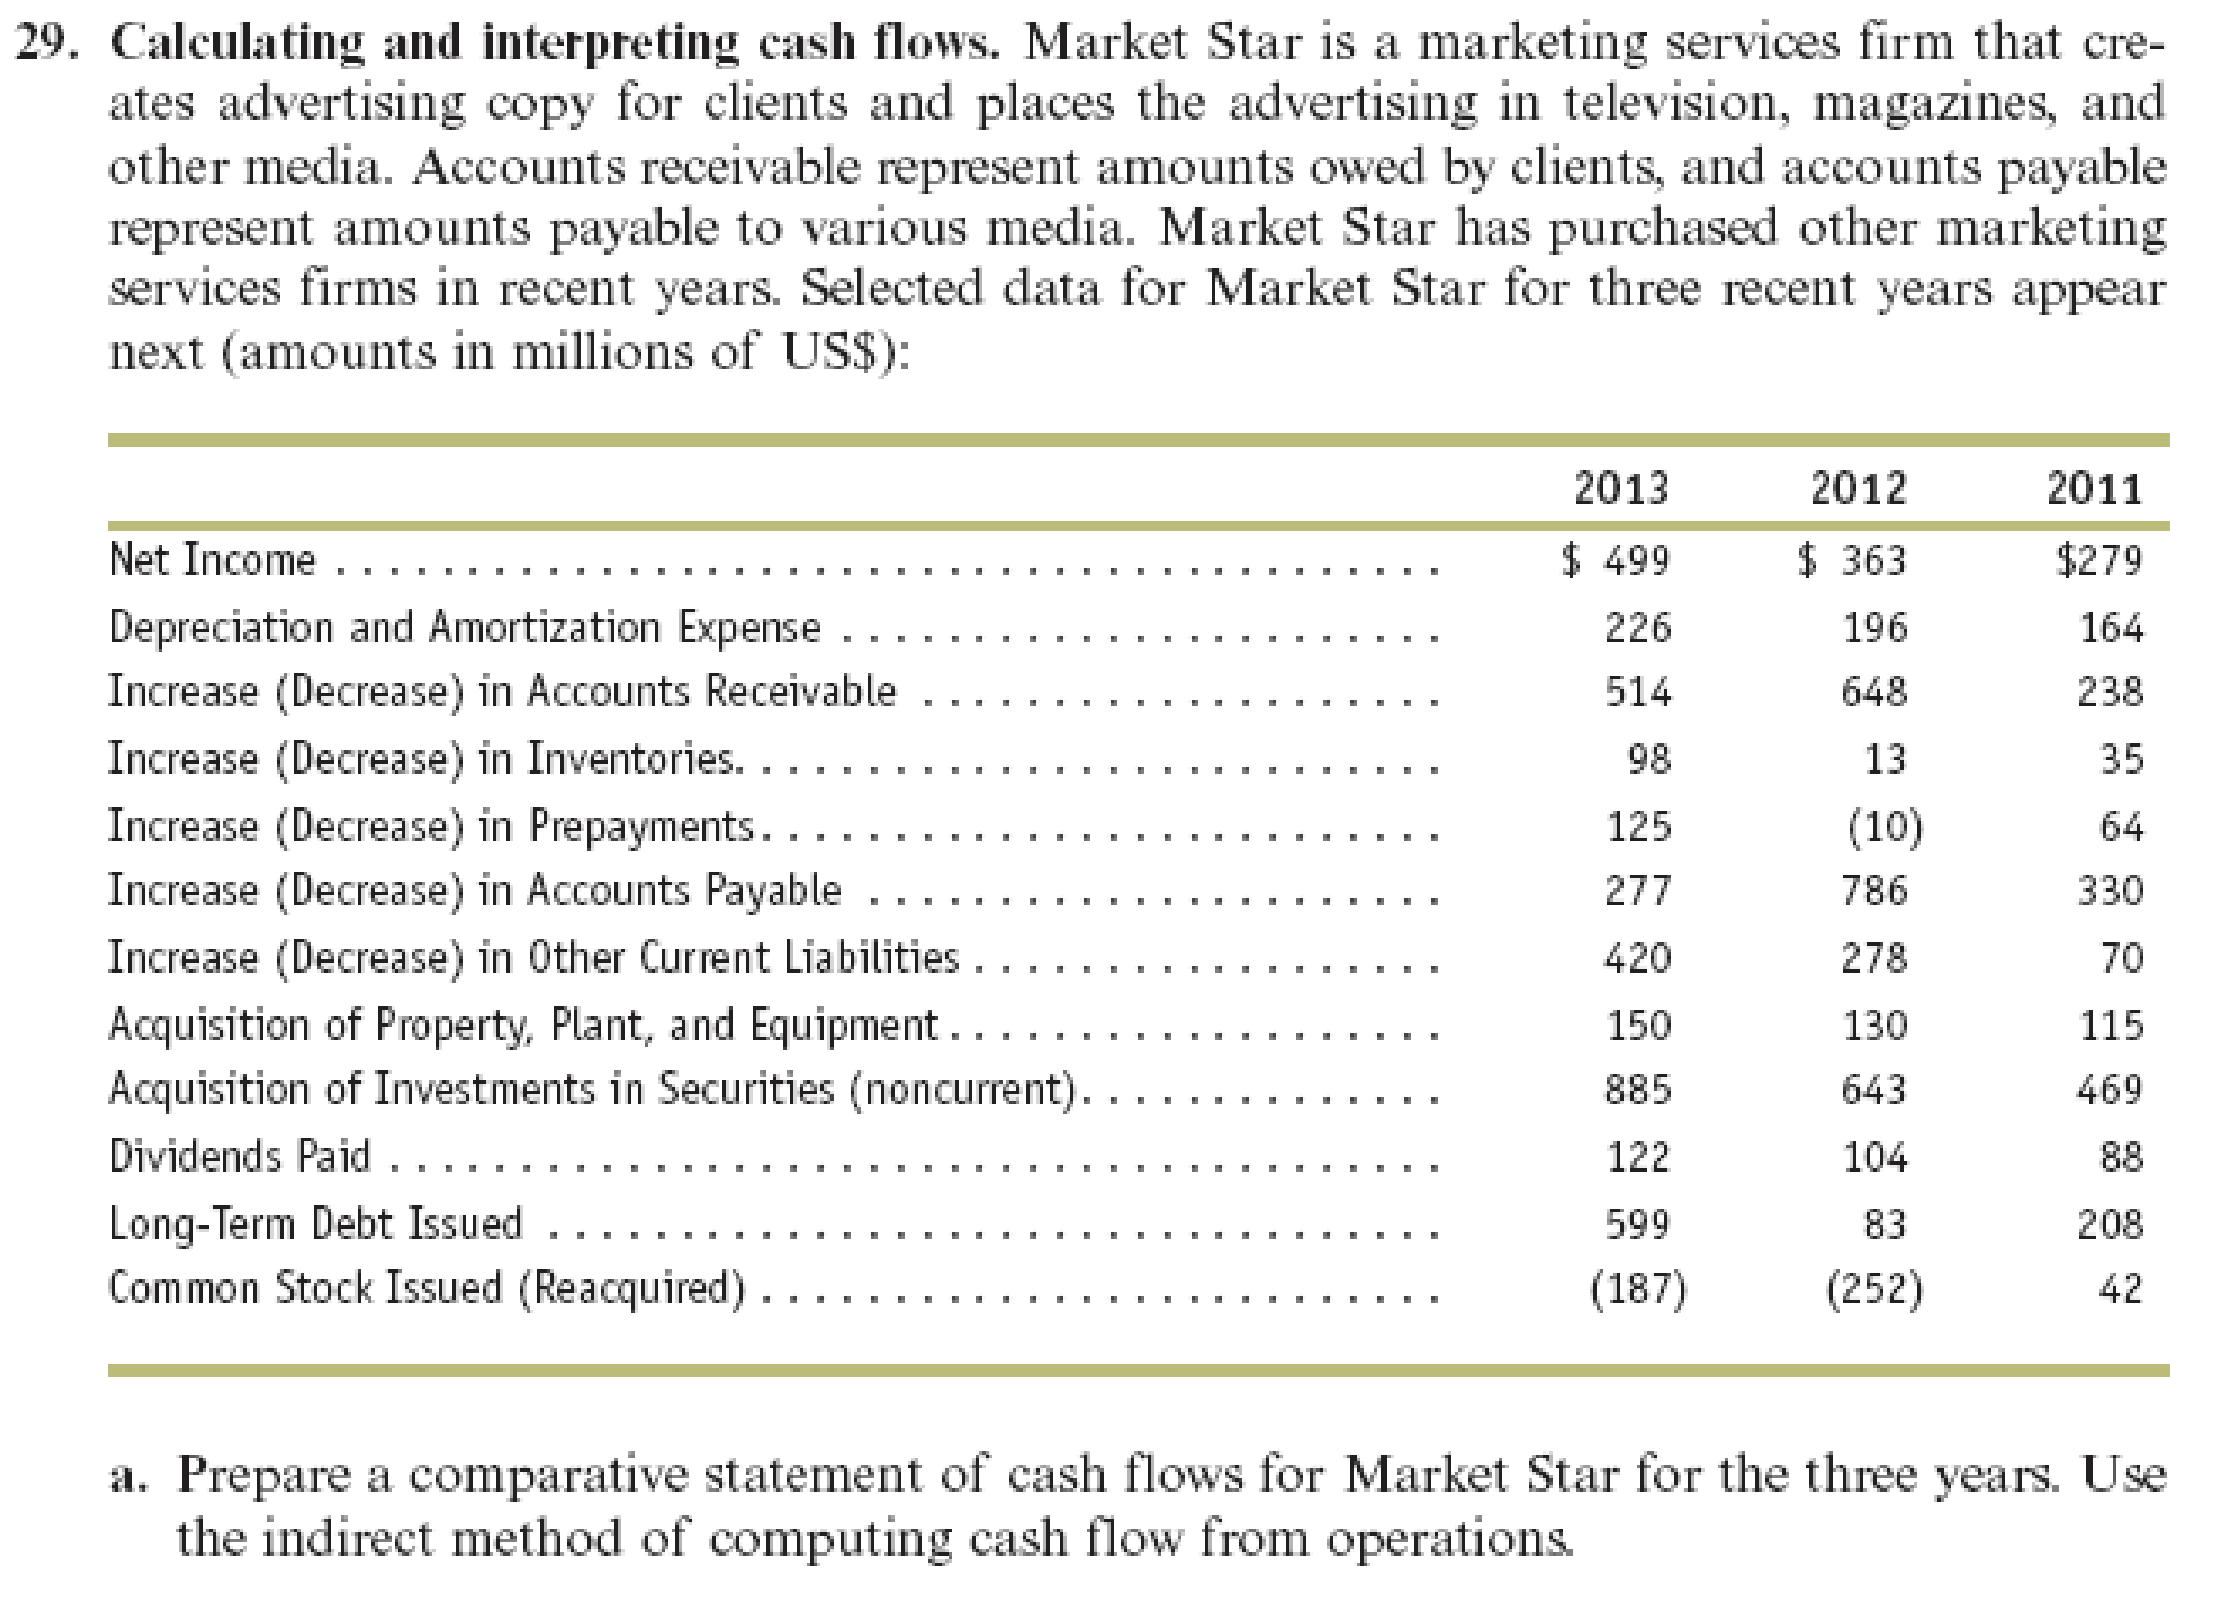
\includegraphics{images/재무회계_6-29.png}

\textbf{\emph{Answer}}

\[Market\;Star\]
\[Statement\;of\;Cash\;Flow\;for\;2011\sim 2013(millions\$)\]

\begin{longtable}[]{@{}clrrr@{}}
\toprule\noalign{}
Category & Name & 2013 & 2012 & 2011 \\
\midrule\noalign{}
\endhead
\bottomrule\noalign{}
\endlastfoot
Cashflow from operations & & \textbf{\$685m} & \textbf{\$972m} &
\textbf{\$506m} \\
+ & Net income & 499 & 363 & 279 \\
+ & Increase in depreciation and amortizaion & 226 & 196 & 279 \\
+ & Increase in account payable & 277 & 786 & 330 \\
- & Increase in account receivable & 514 & 648 & 238 \\
- & Increase in other current liabilities & 420 & 278 & 70 \\
- & Increase in inventories & 98 & 13 & 35 \\
- & Increase in Prepayments & 125 & (10) & 64 \\
Cashflow from investing & & \textbf{(\$1,035)} & \textbf{(\$773)} &
\textbf{(\$584)} \\
- & Increase in property, plant, equipment & 150 & 130 & 115 \\
- & Increase in investments in securities & 885 & 643 & 469 \\
Cashflow from financing & & \textbf{\$290} & \textbf{(\$273)} &
\textbf{\$162} \\
+ & Increasing in long-term debt & 599 & 83 & 208 \\
+ & Increasing in common stock & (187) & (252) & 42 \\
- & Payment of dividends & 122 & 104 & 88 \\
\textbf{Net Change in Cash} & & \textbf{(\$60)} & \textbf{(\$74)} &
\textbf{\$84} \\
\end{longtable}

\chapter*{재무회계 Ch8
과제}\label{uxc7acuxbb34uxd68cuxacc4-ch8-uxacfcuxc81c}
\addcontentsline{toc}{chapter}{재무회계 Ch8 과제}

\markboth{재무회계 Ch8 과제}{재무회계 Ch8 과제}

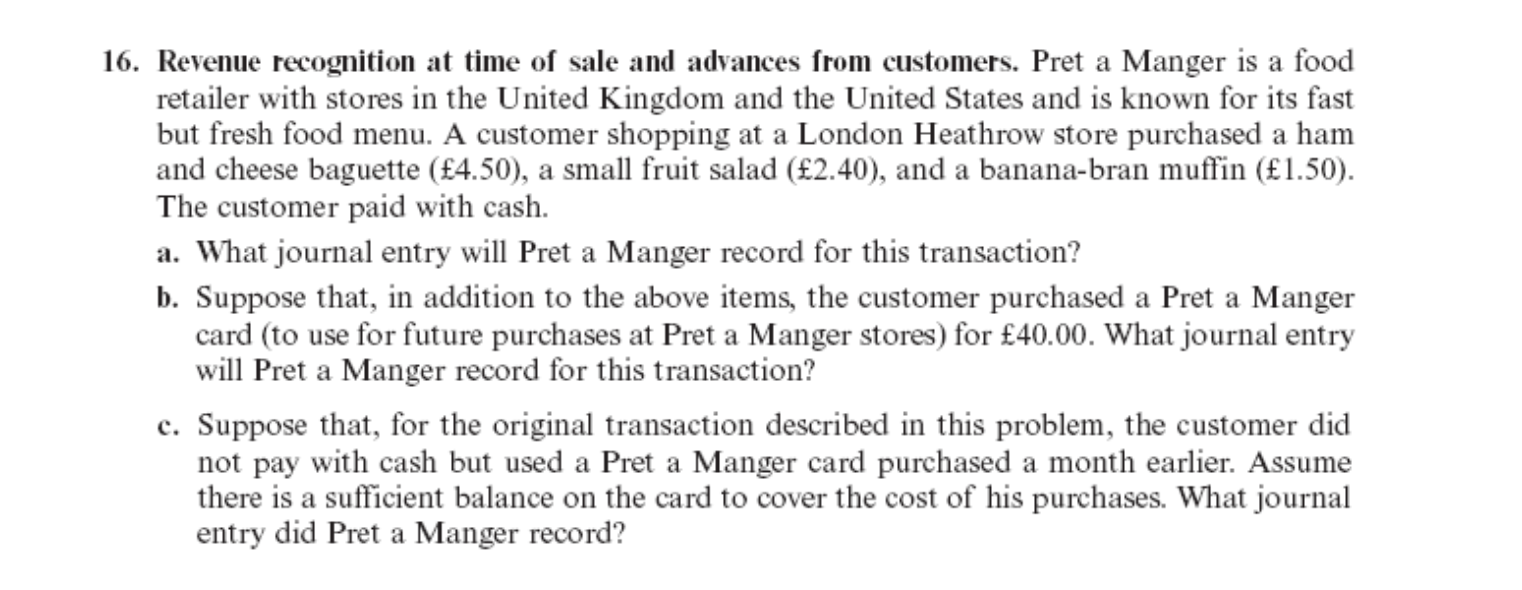
\includegraphics{images/재무회계8-16.png}

\textbf{\emph{Answer}}

\textbf{\emph{(a)}}

debit : cash EUR 8.4

credit : revenue EUR 8.4

\textbf{\emph{(b)}}

debit : cash EUR 48.4

credit : revenue EUR 8.4 / advances from customer EUR 40

\textbf{\emph{(c)}}

debit : advances from customer EUR 8.4

credit : revenue EUR 8.4

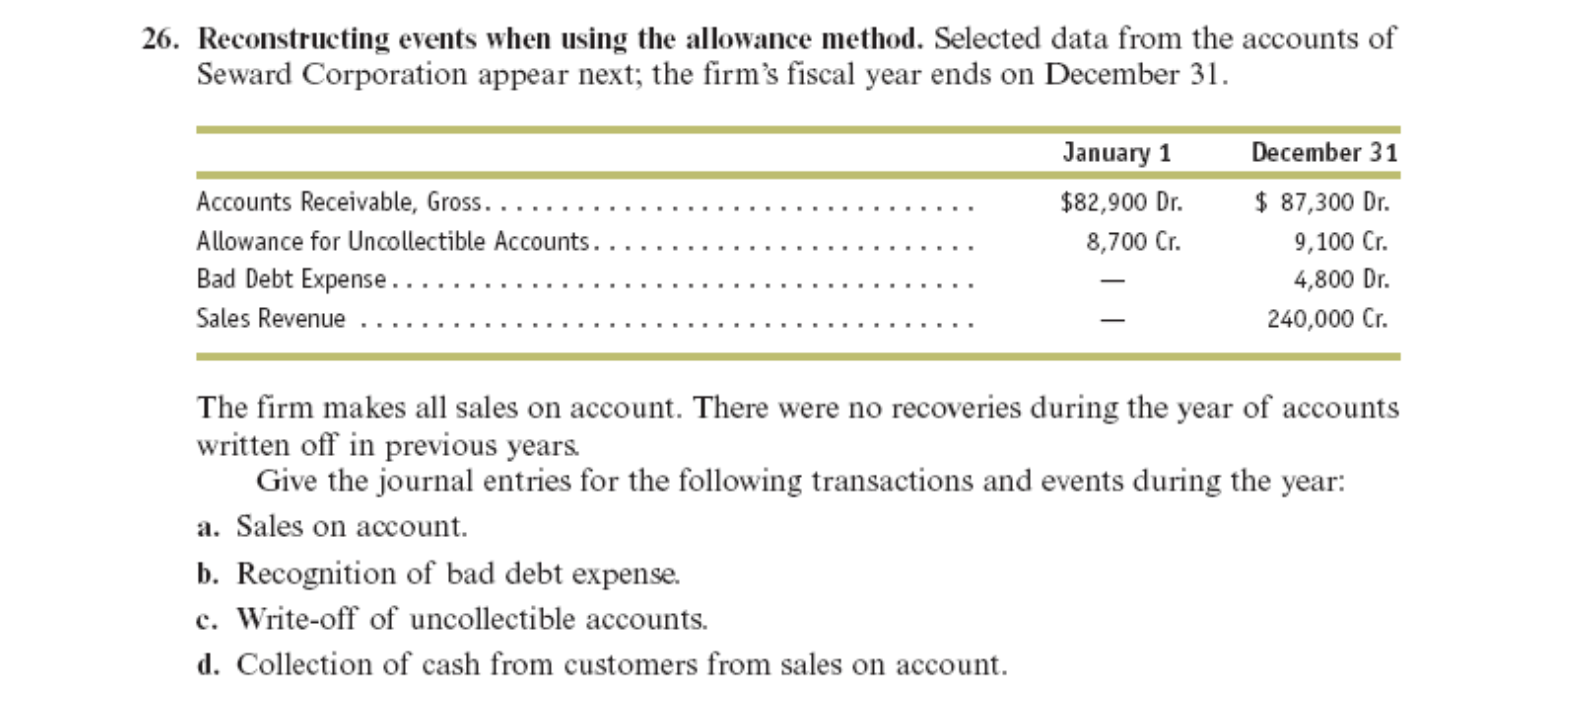
\includegraphics{images/재무회계8-26.png}

\textbf{\emph{(a)}}

debit : account receivable USD 240,000

credit : sales revenue UST 240,000

\textbf{\emph{(b)}}

debit : bad debt expense USD 4,800

credit : allowance for uncollectible accounts USD 4,800

\textbf{\emph{(c)}}

debit : allowance for uncollectible accounts USD 4,400

credit : account receivable USD 4,400

\textbf{\emph{(d)}}

debit : cash USD 231,200

credit : account receivavle USD 231,200

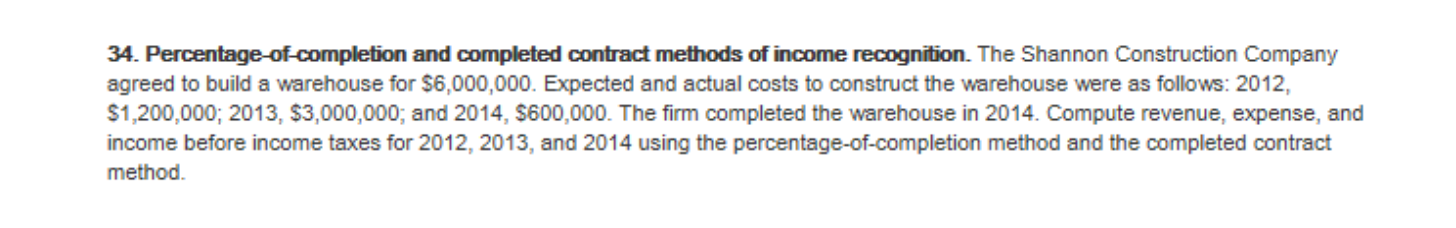
\includegraphics{images/재무회계8-34.png}

\begin{longtable}[]{@{}crrr@{}}
\toprule\noalign{}
category & 2014 & 2013 & 2012 \\
\midrule\noalign{}
\endhead
\bottomrule\noalign{}
\endlastfoot
Cost & 600000 & 3000000 & 1200000 \\
Ratio & 12.5\% & 62.5\% & 25.0\% \\
Revenue & 750000 & 3750000 & 1500000 \\
Income & 150000 & 750000 & 300000 \\
\end{longtable}

\chapter*{재무회계 Ch9
과제}\label{uxc7acuxbb34uxd68cuxacc4-ch9-uxacfcuxc81c}
\addcontentsline{toc}{chapter}{재무회계 Ch9 과제}

\markboth{재무회계 Ch9 과제}{재무회계 Ch9 과제}

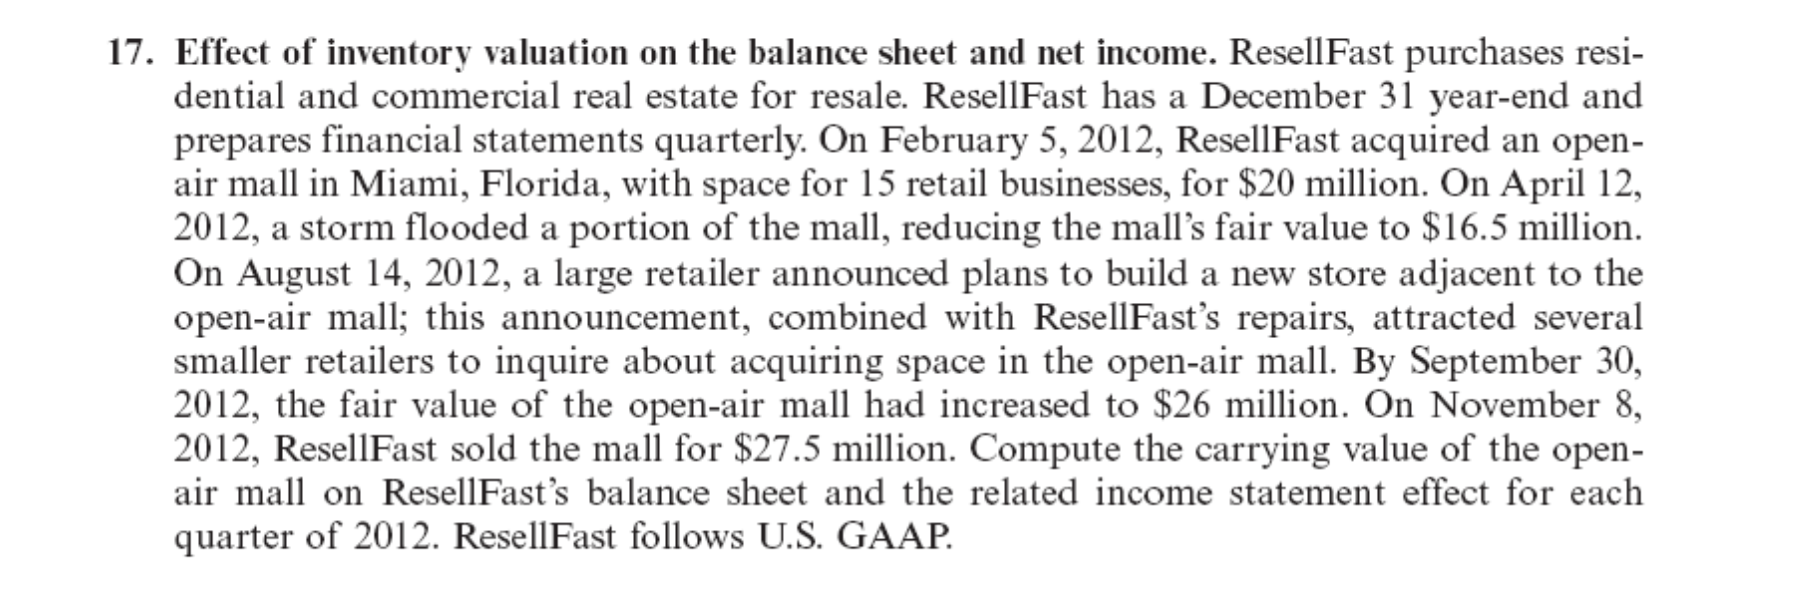
\includegraphics{images/재무회계9-17.png}

\textbf{\emph{Answer}}

\begin{longtable}[]{@{}crr@{}}
\toprule\noalign{}
Category & Inventory & Income \\
\midrule\noalign{}
\endhead
\bottomrule\noalign{}
\endlastfoot
Querter 1 & USD 20m & - \\
Querter 2 & USD 16.5m & -USD 3.5m \\
Querter 3 & USD 16.5m & - \\
Querter 4 & - & +USD 11m \\
\end{longtable}

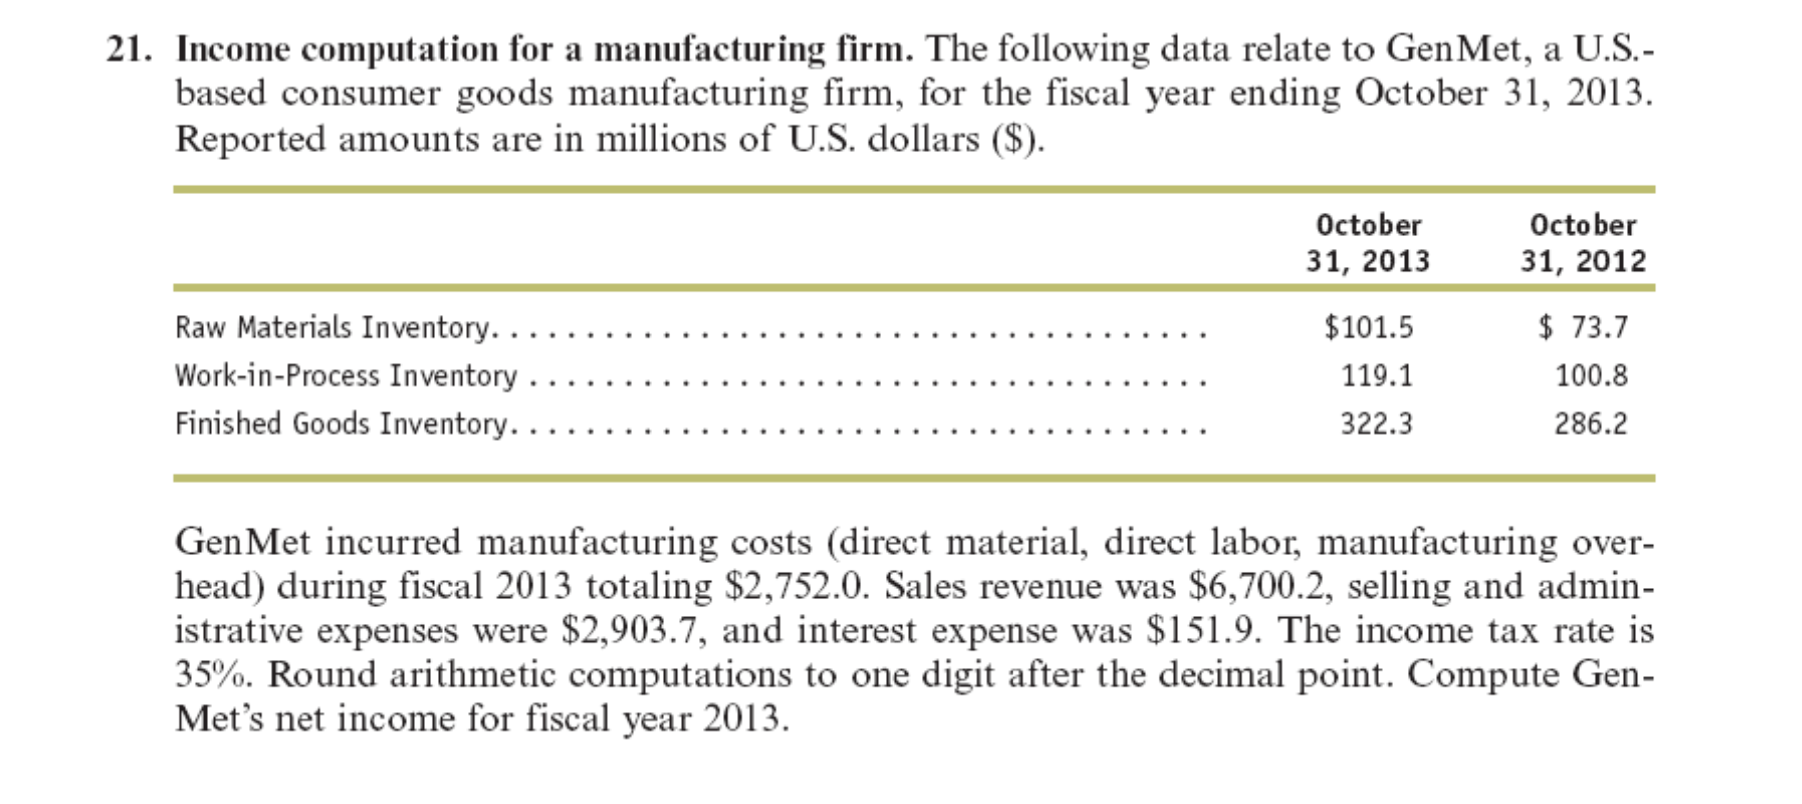
\includegraphics{images/재무회계9-21.png}

\begin{longtable}[]{@{}cr@{}}
\toprule\noalign{}
Cost of sold & Amount(m\$) \\
\midrule\noalign{}
\endhead
\bottomrule\noalign{}
\endlastfoot
Total manufacturing cost & 2752.0 \\
Work in process inventory & 100.8-119.1=(18.3) \\
Finished goods inventory & 286.2-322.3=(36.1) \\
Cost of sold & 2697.6 \\
\end{longtable}

\begin{longtable}[]{@{}cr@{}}
\toprule\noalign{}
Net income & Amount(m\$) \\
\midrule\noalign{}
\endhead
\bottomrule\noalign{}
\endlastfoot
Sales & 6700.2 \\
Cost of sold & (2697.6) \\
Selling and ad. expenses & (2903.7) \\
Interest expense & (151.9) \\
Income tax & 947*35\%=(331.5) \\
\textbf{Net income} & \textbf{615.5} \\
\end{longtable}

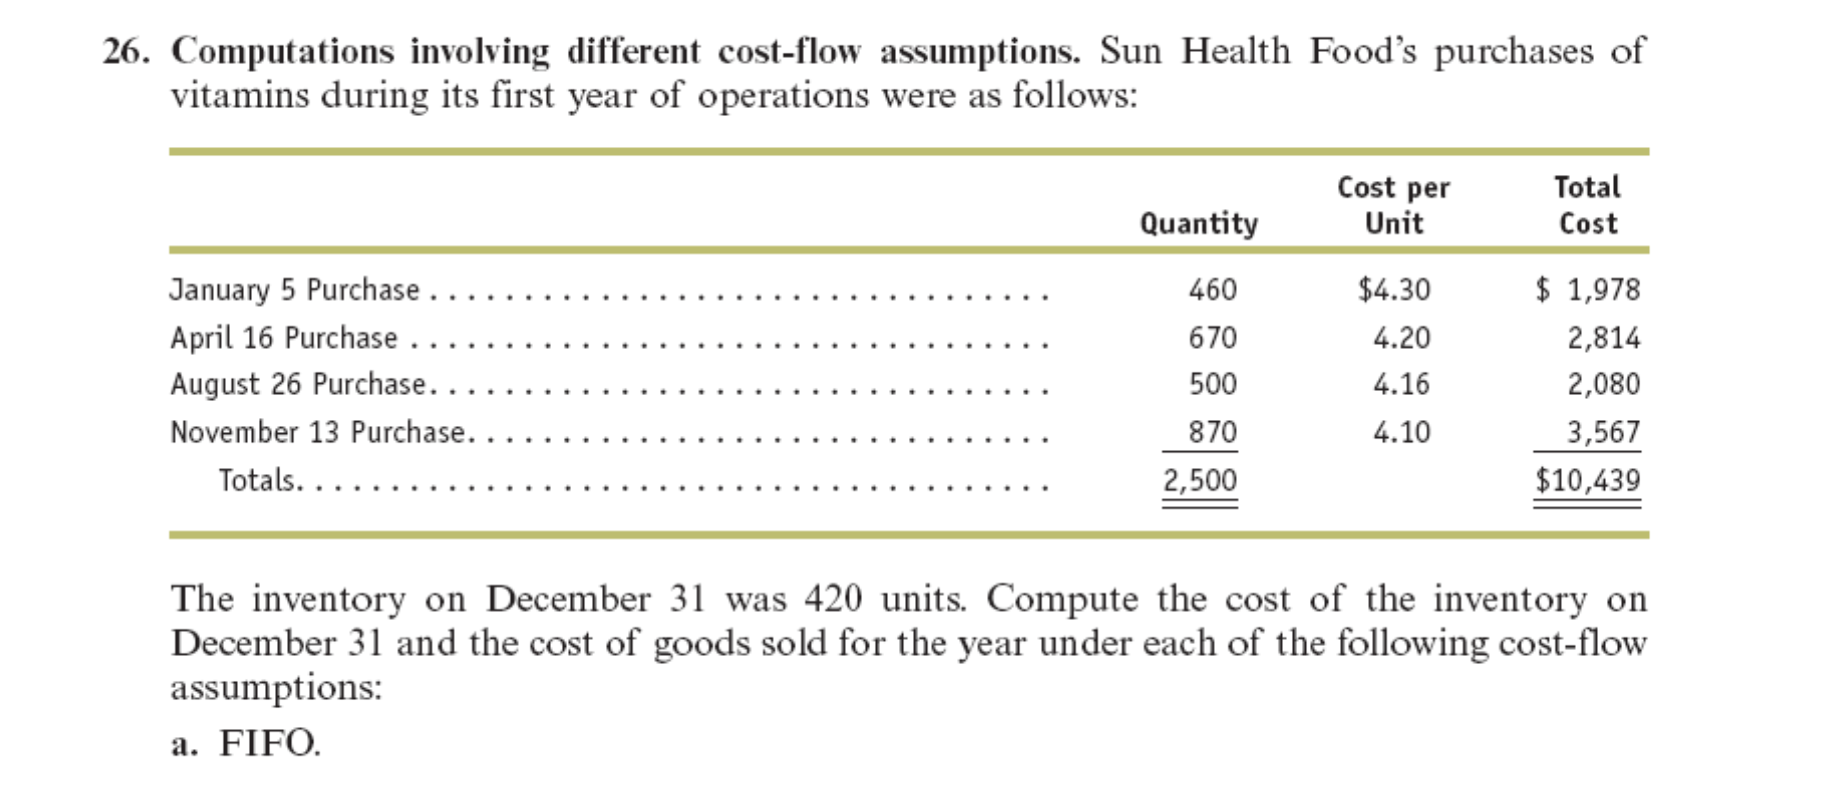
\includegraphics{images/재무회계9-26.png}

The amount of sales is 2080.

Under FIFO, cost will be : \(1978+2814+2080+450\times 4.1=8717\)

\chapter*{재무회계 Ch10
과제}\label{uxc7acuxbb34uxd68cuxacc4-ch10-uxacfcuxc81c}
\addcontentsline{toc}{chapter}{재무회계 Ch10 과제}

\markboth{재무회계 Ch10 과제}{재무회계 Ch10 과제}

\section*{Problem 10-21}\label{problem-10-21}
\addcontentsline{toc}{section}{Problem 10-21}

\markright{Problem 10-21}

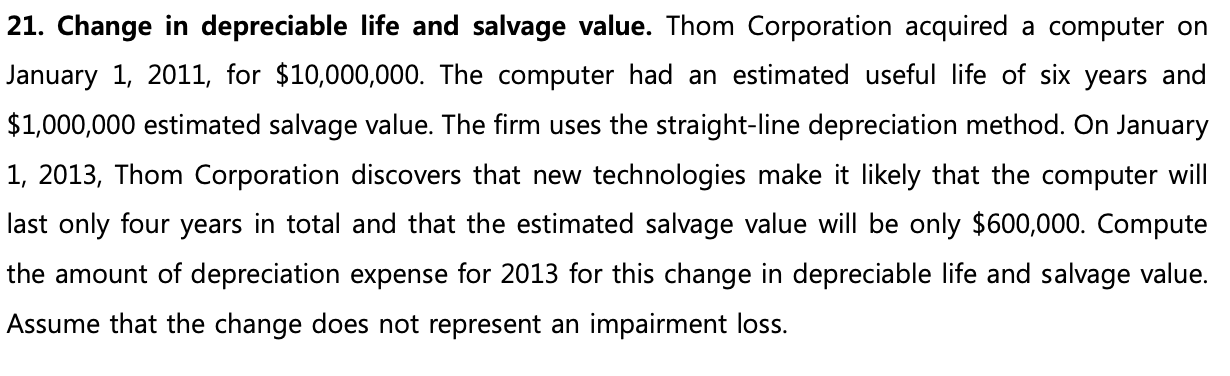
\includegraphics{images/재무회계_10-21.png}

\subsection*{Answer}\label{answer-16}
\addcontentsline{toc}{subsection}{Answer}

Carrying value :
\(10,000,000-(2\times\frac{10,000,000-1,000,000}{6})=7,000,000USD\)

Depreciation : \(\frac{7,000,000-600,000}{2}=3,200,000USD\)

\section*{Problem 10-29}\label{problem-10-29}
\addcontentsline{toc}{section}{Problem 10-29}

\markright{Problem 10-29}

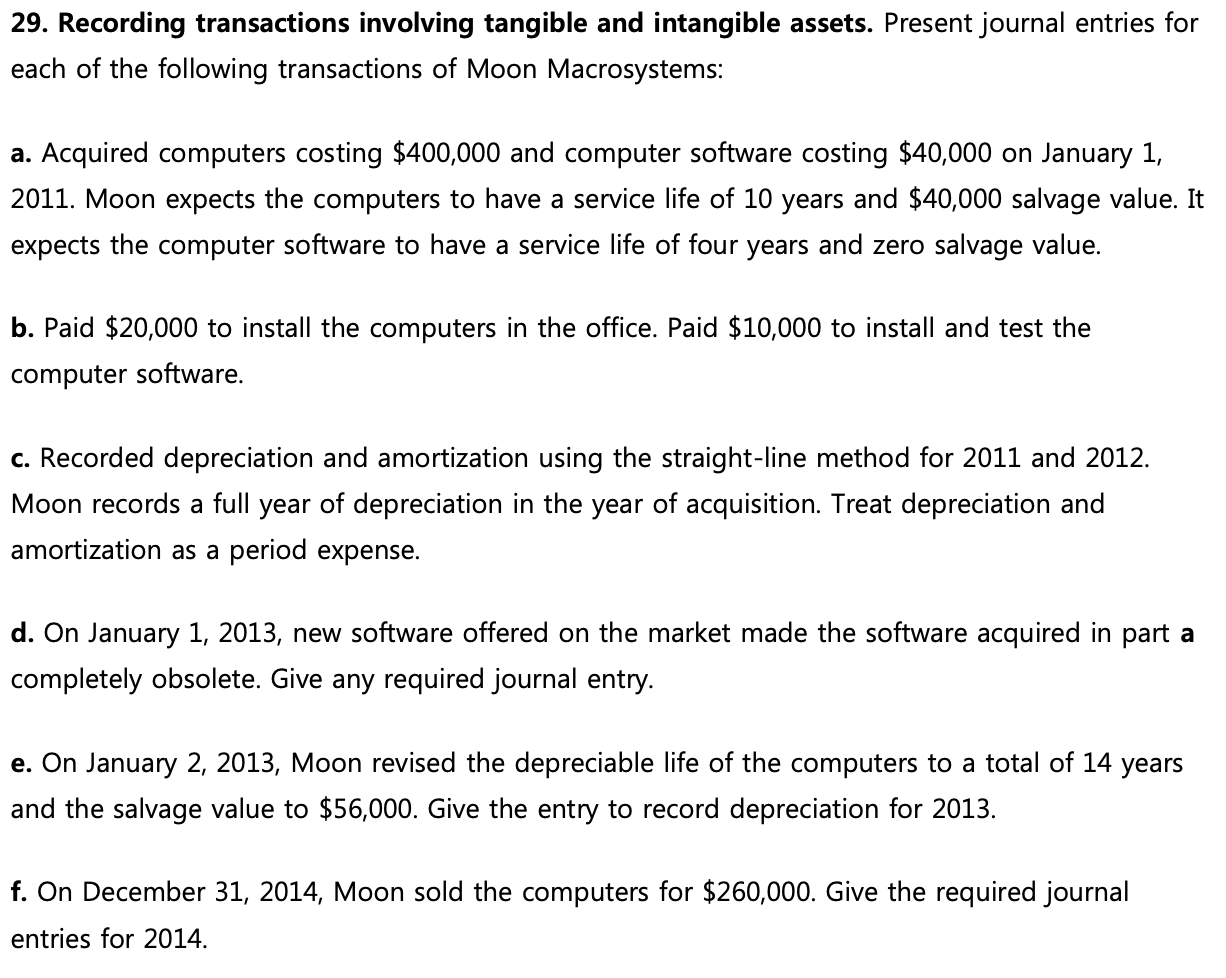
\includegraphics{images/재무회계_10-29.png}

\subsection*{Answer}\label{answer-17}
\addcontentsline{toc}{subsection}{Answer}

\subsubsection*{(a)}\label{a-1}
\addcontentsline{toc}{subsubsection}{(a)}

debit : Computer 400,000 / Software 40,000

credit : Cash 440,000

\subsubsection*{(b)}\label{b-1}
\addcontentsline{toc}{subsubsection}{(b)}

debit : Computer 20,000 / Software 10,000

credit : Cash 30,000

\subsubsection*{(c)}\label{c}
\addcontentsline{toc}{subsubsection}{(c)}

debit : Depreciation 76,000(=2\emph{(420000-40000)/10) / Amortization
25,000(=2}50000/4)

credit : Accumulated Depreciation 76,000 / Software 25,000

\subsubsection*{(d)}\label{d}
\addcontentsline{toc}{subsubsection}{(d)}

debit : Loss of software 25,000

credit : Software 25,000

\subsubsection*{(e)}\label{e}
\addcontentsline{toc}{subsubsection}{(e)}

debit : Depreciation 24,000(=(420000-38000*2-56000)/12)

credit : Accumulated depreciation 24,000

\subsubsection*{(f)}\label{f}
\addcontentsline{toc}{subsubsection}{(f)}

debit : Depreciation 24,000 / Cash 260,000 / Accumulated depreciation
124,000 / Loss of computer 36,000

credit : Accumulated depreciation 24,000 / Computer 420,000

\chapter*{재무회계 Ch11
과제}\label{uxc7acuxbb34uxd68cuxacc4-ch11-uxacfcuxc81c}
\addcontentsline{toc}{chapter}{재무회계 Ch11 과제}

\markboth{재무회계 Ch11 과제}{재무회계 Ch11 과제}

\section*{Problem 11-18.}\label{problem-11-18.}
\addcontentsline{toc}{section}{Problem 11-18.}

\markright{Problem 11-18.}

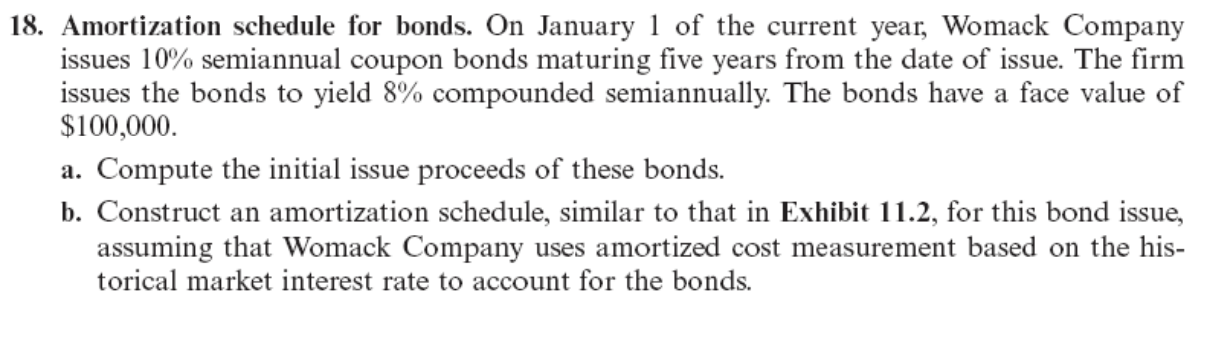
\includegraphics{images/재무회계_11-18.png}

\subsection*{Answer}\label{answer-18}
\addcontentsline{toc}{subsection}{Answer}

\section*{Problem 11-19.}\label{problem-11-19.}
\addcontentsline{toc}{section}{Problem 11-19.}

\markright{Problem 11-19.}

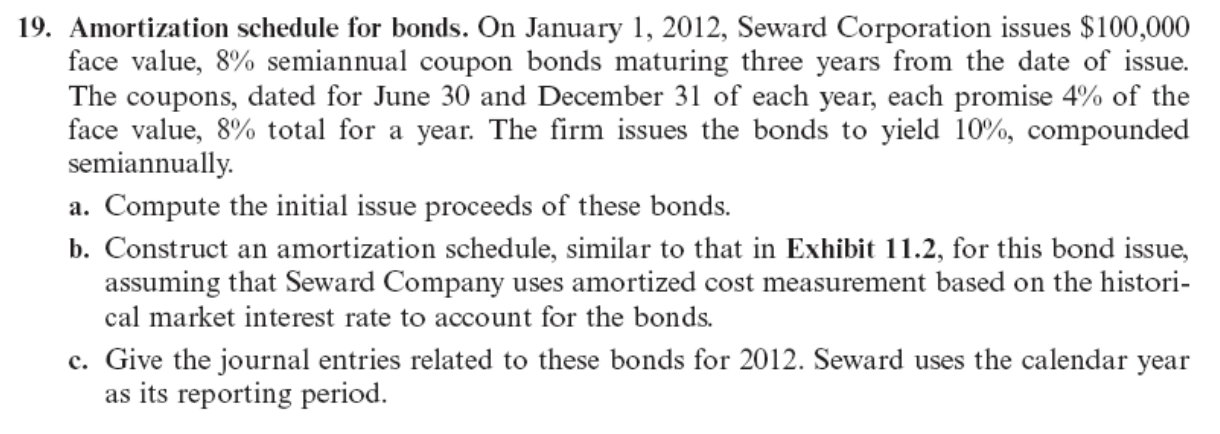
\includegraphics{images/재무회계_11-19.png}

\section*{Exhibit 11.2}\label{exhibit-11.2}
\addcontentsline{toc}{section}{Exhibit 11.2}

\markright{Exhibit 11.2}

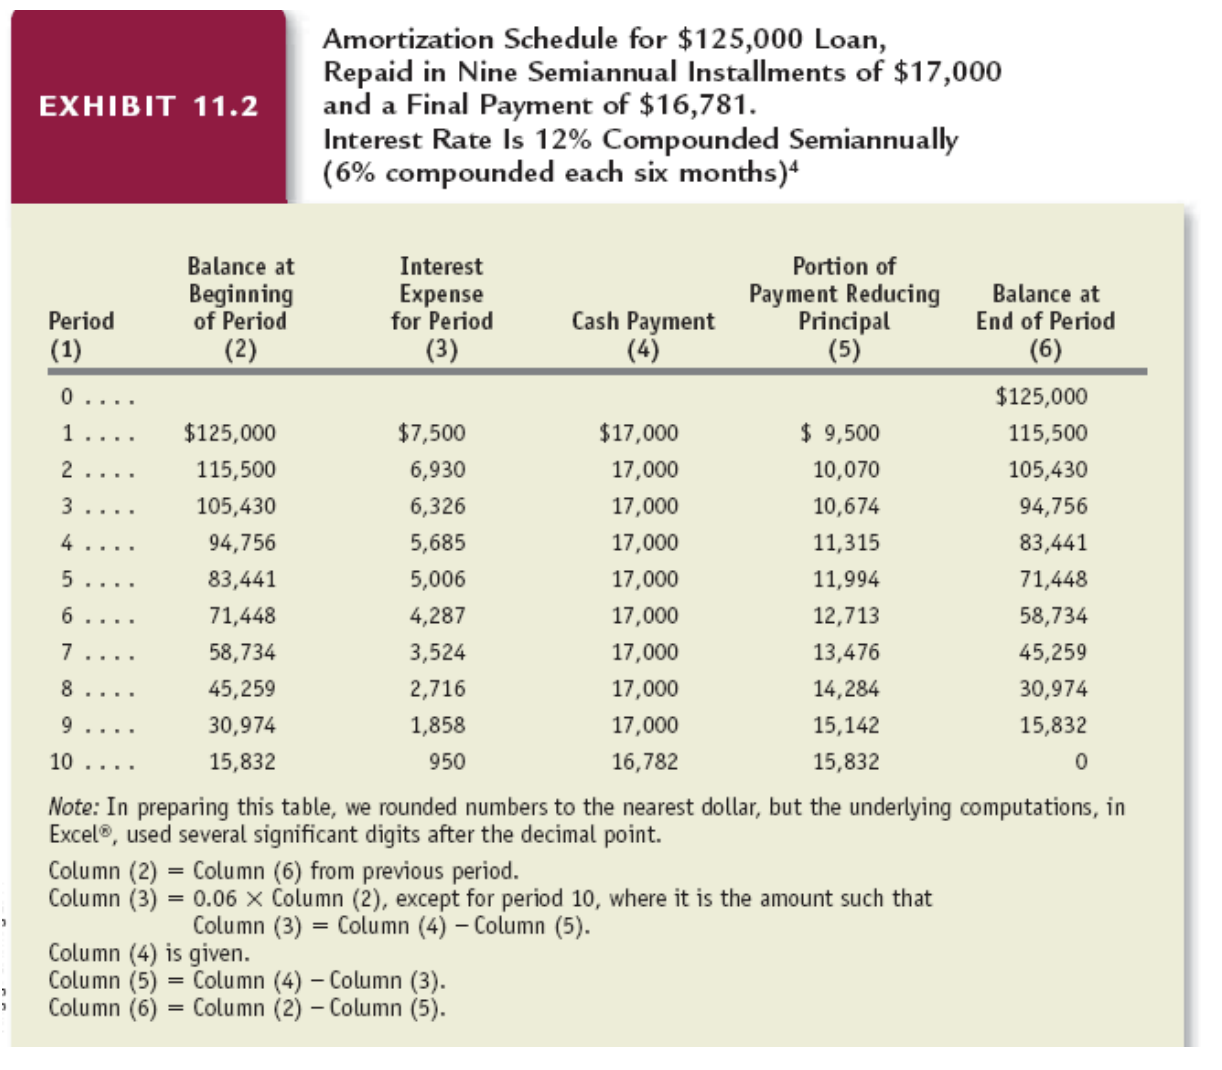
\includegraphics{images/재무회계_11-19b.png}

\part{경영통계분석('24봄)}

\chapter*{경영통계분석
과제1}\label{uxacbduxc601uxd1b5uxacc4uxbd84uxc11d-uxacfcuxc81c1}
\addcontentsline{toc}{chapter}{경영통계분석 과제1}

\markboth{경영통계분석 과제1}{경영통계분석 과제1}

\section*{1. Type of variables}\label{type-of-variables}
\addcontentsline{toc}{section}{1. Type of variables}

\markright{1. Type of variables}

\textbf{\emph{Question}}

Identify whether the following variables are numerical or categorical.
If numerical, state whether the variable is discrete or continuous. If
categorical, state whether the variable is nominal or ordinal.

\textbf{a. Number of companies going bankrupt in a year.}

: Numerical and Discrete

\textbf{b. Petal area of rose flowers.}

: Numerical and Continuous

\textbf{c.~Key on the musical scale.}

: Categorical and Ordinal

\textbf{d.~Heart beats per minute of a Tour de France cyclist, averaged
over the duration of the race.}

: Numerical and Continuous

\textbf{e. Stage of fruit ripeness.}

: Categorical and Ordinal

\textbf{f.~Angle of flower orientation relative to position of the sun.}

: Numerical and Continuous

\textbf{g. Tree species}

: Categorical and Nominal

\textbf{h. year of birth}

: Numerical and Discrete

\textbf{i. Gender}

: Categorical and Nominal

\textbf{j. Birth weight}

: Numerical and Continuous

\section*{2. Discrete data}\label{discrete-data}
\addcontentsline{toc}{section}{2. Discrete data}

\markright{2. Discrete data}

\textbf{\emph{Question}}

Birds of the Caribbean islands of the Lesser Antilles are descended from
immigrants originating from larger islands and the nearby mainland. The
data presented here are the approximate dates of immigration, in
millions of years, of each of 37 bird species now present on the Lesser
Antilles. The dates were calculated from the difference in mitochondrial
DNA sequences between each of the species and its closest living
relative on larger islands or the mainland.

\begin{Shaded}
\begin{Highlighting}[]
\FunctionTok{library}\NormalTok{(tidyverse)}
\NormalTok{birds\_caribbean }\OtherTok{\textless{}{-}} \FunctionTok{tibble}\NormalTok{(}\StringTok{"dates"}\OtherTok{=}\FunctionTok{c}\NormalTok{(}\FloatTok{0.00}\NormalTok{,}\FloatTok{0.00}\NormalTok{,}\FloatTok{0.04}\NormalTok{,}\FloatTok{0.21}\NormalTok{,}\FloatTok{0.29}\NormalTok{,}
\FloatTok{0.54}\NormalTok{,}\FloatTok{0.63}\NormalTok{,}\FloatTok{0.88}\NormalTok{,}\FloatTok{0.96}\NormalTok{,}\FloatTok{1.25}\NormalTok{,}
\FloatTok{1.67}\NormalTok{,}\FloatTok{1.75}\NormalTok{,}\FloatTok{1.84}\NormalTok{,}\FloatTok{1.96}\NormalTok{,}\FloatTok{2.01}\NormalTok{,}
\FloatTok{2.51}\NormalTok{,}\FloatTok{2.72}\NormalTok{,}\FloatTok{3.30}\NormalTok{,}\FloatTok{3.51}\NormalTok{,}\FloatTok{4.05}\NormalTok{,}
\FloatTok{4.85}\NormalTok{,}\FloatTok{6.94}\NormalTok{,}\FloatTok{8.73}\NormalTok{,}\FloatTok{10.57}\NormalTok{,}\FloatTok{11.11}\NormalTok{,}
\FloatTok{12.45}\NormalTok{,}\FloatTok{14.00}\NormalTok{,}\FloatTok{17.30}\NormalTok{,}\FloatTok{17.92}\NormalTok{,}\FloatTok{18.05}\NormalTok{,}
\FloatTok{18.43}\NormalTok{,}\FloatTok{22.48}\NormalTok{,}\FloatTok{22.48}\NormalTok{,}\FloatTok{23.48}\NormalTok{,}\FloatTok{26.32}\NormalTok{,}
\FloatTok{26.45}\NormalTok{,}\FloatTok{28.87}\NormalTok{))}
\end{Highlighting}
\end{Shaded}

\begin{Shaded}
\begin{Highlighting}[]
\NormalTok{birds\_caribbean}\SpecialCharTok{$}\NormalTok{dates}
\end{Highlighting}
\end{Shaded}

\begin{verbatim}
 [1]  0.00  0.00  0.04  0.21  0.29  0.54  0.63  0.88  0.96  1.25  1.67  1.75
[13]  1.84  1.96  2.01  2.51  2.72  3.30  3.51  4.05  4.85  6.94  8.73 10.57
[25] 11.11 12.45 14.00 17.30 17.92 18.05 18.43 22.48 22.48 23.48 26.32 26.45
[37] 28.87
\end{verbatim}

\textbf{a. Plot the data in a histogram and describe the shape of the
frequency distribution.}

\begin{Shaded}
\begin{Highlighting}[]
\FunctionTok{ggplot}\NormalTok{(}\AttributeTok{data=}\NormalTok{birds\_caribbean, }\FunctionTok{aes}\NormalTok{(}\AttributeTok{x=}\NormalTok{dates))}\SpecialCharTok{+}
  \FunctionTok{geom\_histogram}\NormalTok{(}\AttributeTok{binwidth=}\DecValTok{5}\NormalTok{, }\AttributeTok{boundary=}\DecValTok{0}\NormalTok{, }\AttributeTok{color=}\StringTok{"black"}\NormalTok{,}\AttributeTok{fill=}\StringTok{"darkred"}\NormalTok{)}\SpecialCharTok{+}
  \FunctionTok{scale\_x\_continuous}\NormalTok{(}\AttributeTok{breaks =} \FunctionTok{seq}\NormalTok{(}\DecValTok{0}\NormalTok{,}\DecValTok{30}\NormalTok{,}\DecValTok{5}\NormalTok{)) }\SpecialCharTok{+}
  \FunctionTok{theme\_bw}\NormalTok{()}
\end{Highlighting}
\end{Shaded}

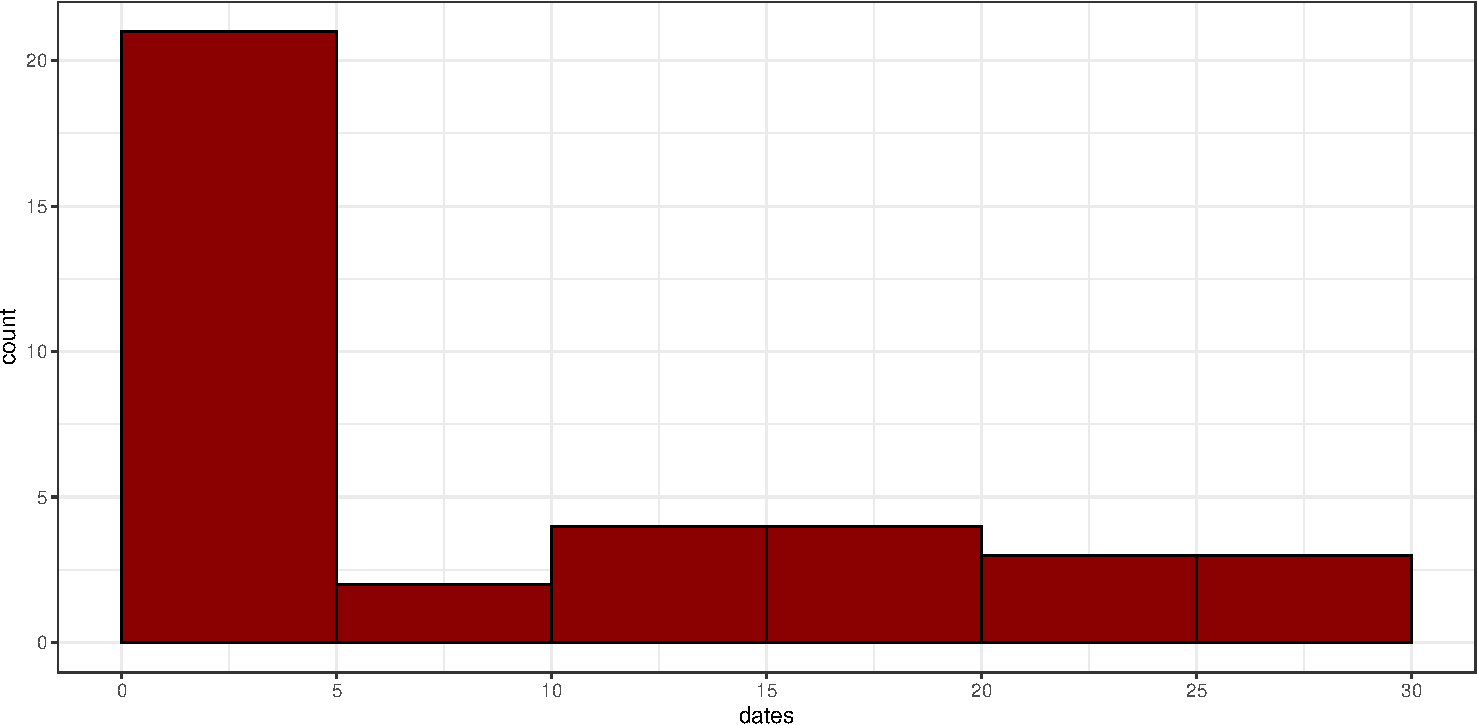
\includegraphics{경영통계분석_hw1_files/figure-pdf/unnamed-chunk-3-1.pdf}

히스토그램은 위와 같으며, 0\textasciitilde5구간에 전체 37종의 조류 중
20종 이상이 넘는 빈도가 집중되어 있습니다. 이는 과반 이상의 조류가
비교적 최근인 500만년 이내에 Lesser Antilles섬으로 이주해왔다는 것을
의미합니다. 나머지 약 15종의 조류는 각각 2\textasciitilde4종씩
\textasciitilde1천만년, \textasciitilde1500만년, \ldots{} ,
\textasciitilde3천만년 구간에 고르게 분포되어 있습니다.

\textbf{b. By viewing the graph alone, approximate the mean and median
of the distribution. Which should be greater? Explain your reasoning.}

: 히스토그램은 왼쪽으로 치우쳐져 있으며, 이는 \(Skewness>>0\)이라는 것을
말합니다. 이러한 경우 평균은 중간값보다 크게 형성되고, 오른쪽 꼬리가
다소 긴 점을 감안하여 추정해보면, \textbf{중간값은 약 4, 평균은 약 10}일
것으로 보입니다.

\textbf{c.~Calculate the mean and median. Was your intuition in part (b)
correct?}

\begin{Shaded}
\begin{Highlighting}[]
\NormalTok{birds\_caribbean }\SpecialCharTok{\%\textgreater{}\%} 
  \FunctionTok{summarise}\NormalTok{(}\AttributeTok{mean=}\FunctionTok{mean}\NormalTok{(dates),}
            \AttributeTok{mid=}\FunctionTok{median}\NormalTok{(dates))}
\end{Highlighting}
\end{Shaded}

\begin{verbatim}
# A tibble: 1 x 2
   mean   mid
  <dbl> <dbl>
1  8.66  3.51
\end{verbatim}

: 대략적인 경향성은 맞습니다. 실제 중간값은 3.51 및 평균은 8.66입니다.

\textbf{d.~Calculate the first and third quantiles and the inter
quartile range.}

\begin{Shaded}
\begin{Highlighting}[]
\NormalTok{birds\_caribbean }\SpecialCharTok{\%\textgreater{}\%} 
  \FunctionTok{reframe}\NormalTok{(}\AttributeTok{quantile=}\FunctionTok{quantile}\NormalTok{(dates))}
\end{Highlighting}
\end{Shaded}

\begin{verbatim}
# A tibble: 5 x 1
  quantile
     <dbl>
1     0   
2     1.25
3     3.51
4    17.3 
5    28.9 
\end{verbatim}

: First(25\%) quantiles은 1.25이며, third(75\%) quantiles은 17.30입니다.
IQR은 16.05입니다.

\textbf{e. Draw a box plot for these data}

\begin{Shaded}
\begin{Highlighting}[]
\FunctionTok{ggplot}\NormalTok{(birds\_caribbean, }\FunctionTok{aes}\NormalTok{(}\AttributeTok{x=}\NormalTok{dates))}\SpecialCharTok{+}
  \FunctionTok{geom\_boxplot}\NormalTok{()}\SpecialCharTok{+}
  \FunctionTok{scale\_y\_continuous}\NormalTok{(}\AttributeTok{limits=}\FunctionTok{c}\NormalTok{(}\SpecialCharTok{{-}}\FloatTok{0.5}\NormalTok{,}\FloatTok{0.5}\NormalTok{))}\SpecialCharTok{+}
  \FunctionTok{theme\_bw}\NormalTok{()}
\end{Highlighting}
\end{Shaded}

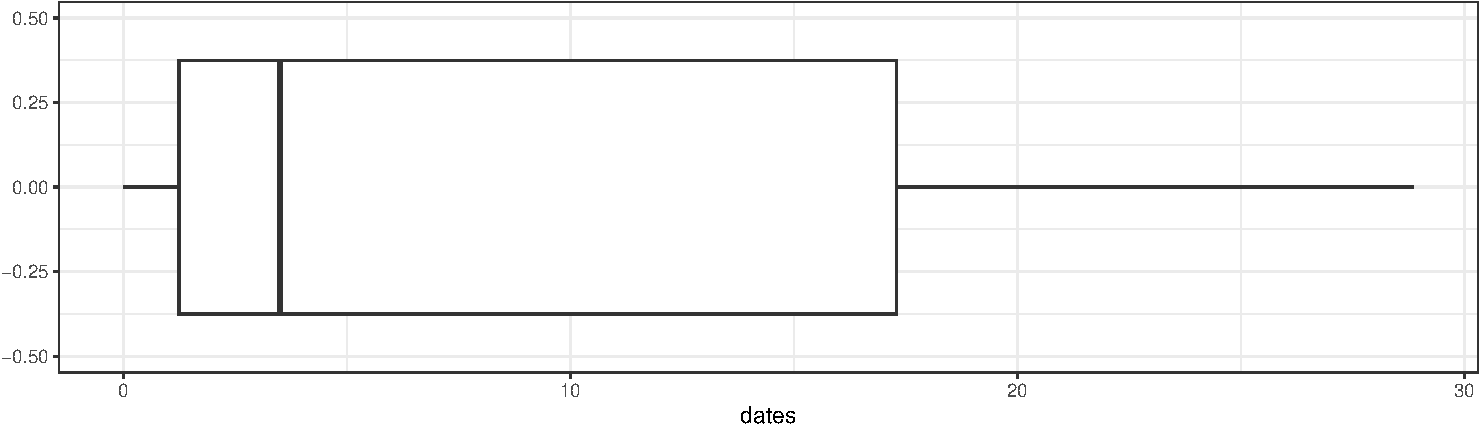
\includegraphics{경영통계분석_hw1_files/figure-pdf/unnamed-chunk-6-1.pdf}

\section*{3. Histogram}\label{histogram}
\addcontentsline{toc}{section}{3. Histogram}

\markright{3. Histogram}

\textbf{\emph{Question}}

Francis Galton presented the following data on the flight speeds of 3207
``old'' homing pigeons traveling at least 90 miles.

\textbf{a. What type of graph is this?}

: Histogram

\textbf{b. Examine the graph and visually determine the approximate
value of the mean (to the nearest 100 yards per minute). Explain how you
obtained your estimate.}

: 그래프는 bell-shape의 히스토그램이며, 오른쪽 꼬리가 긴 형태입니다.
아마 \(skewness>0\)일 것으로 보이며, 평균은 중간값보다 클 것 입니다.

그래프에서 중간값은 오른쪽 꼬리가 긴 분포를 고려할 때 약 1,000일 것으로
추정할 수 있는데, \textbf{평균값은 이보다 큰 약 1,100}이 될 것으로
추정됩니다.

\textbf{c.~Examine the graph and visually determine the approximate
value of the median (to the nearest 100 yards per minute). Explain how
you obtain your estimate.}

: 그래프에서 900\textasciitilde1000이 중심막대인데, bell-shape와 오른쪽
꼬리가 긴 분포를 고려할 때, \textbf{중간값은 약 1,000}이 될 것으로
추정됩니다.

\textbf{d.~Examine the graph and visually determine the approximate
value of the mode (to the nearest 100 yards per minute). Explain how you
obtained your estimate.}

: 최빈값은 가장 많은 빈도를 가지는 값 또는 구간으로, 히스토그램의 가장
높은 막대인 1000\textasciitilde1100에 존재할 것입니다. 막대 왼쪽에
빈도가 더 많은 점을 고려할 때 \textbf{최빈값은 약 1,000}일 것으로
보입니다.

\textbf{e. Examine the graph and visually determine the approximate
value of the standard deviation (to the nearest 100 yards per minute).
Explain how you obtained your estimate.}

: 먼저, 정규분포를 따르는 확률변수에 대해 다음 식이 성립합니다.

\[for\;X\;\sim\;Normal\;Dist.\;then\;P[-\sigma<X<\sigma]\approx 68.2\%\]

문제의 히스토그램은 bell-shape로 정규분포를 따른다고 가정하는 것에 큰
문제는 없어보입니다. 히스토그램에서 어림잡아봤을 때, 약 \(1,100\pm 200\)
구간이 70\textasciitilde80\%에 해당한다고 보여지는데,
(\(P[900<x<1300]=70\sim80\%\))

이는 (b)의 추정 평균을 이용하면 \(평균\pm 200\)입니다. 즉, 히스토그램이
정규분포를 따른다고 가정하면, 히스토그램의 형태는
\(N(1050,\sigma^2=(200-\alpha)^2)\)의 확률밀도함수가 유사할 것입니다.
한편, 히스토그램은 오른쪽 꼬리가 긴 형태를 가지고 있어 변동성은 정규분포
대비 다소 클 것입니다.

따라서, 최종적으로 \textbf{히스토그램 데이터의 표준편차}는 \textbf{약
200으로 추정}됩니다.

\section*{4. Sample Statistics}\label{sample-statistics}
\addcontentsline{toc}{section}{4. Sample Statistics}

\markright{4. Sample Statistics}

\begin{Shaded}
\begin{Highlighting}[]
\NormalTok{handheight }\OtherTok{\textless{}{-}} \FunctionTok{tibble}\NormalTok{(}\StringTok{"person"}\OtherTok{=}\FunctionTok{c}\NormalTok{(}\StringTok{"A"}\NormalTok{,}\StringTok{"B"}\NormalTok{,}\StringTok{"C"}\NormalTok{,}\StringTok{"D"}\NormalTok{,}\StringTok{"E"}\NormalTok{),}
                     \StringTok{"hand"}\OtherTok{=}\FunctionTok{c}\NormalTok{(}\DecValTok{17}\NormalTok{,}\DecValTok{15}\NormalTok{,}\DecValTok{19}\NormalTok{,}\DecValTok{17}\NormalTok{,}\DecValTok{21}\NormalTok{),}
                     \StringTok{"height"}\OtherTok{=}\FunctionTok{c}\NormalTok{(}\DecValTok{150}\NormalTok{,}\DecValTok{154}\NormalTok{,}\DecValTok{169}\NormalTok{,}\DecValTok{172}\NormalTok{,}\DecValTok{175}\NormalTok{))}
\NormalTok{handheight}
\end{Highlighting}
\end{Shaded}

\begin{verbatim}
# A tibble: 5 x 3
  person  hand height
  <chr>  <dbl>  <dbl>
1 A         17    150
2 B         15    154
3 C         19    169
4 D         17    172
5 E         21    175
\end{verbatim}

\textbf{a. Calculate the sample variances for hand and height,
respectively.}

표분 분산은 \(s_x^2=\frac{\sum_{k=1}^n(X_k-\bar{X})^2}{n-1}\)입니다.

\begin{Shaded}
\begin{Highlighting}[]
\NormalTok{sample\_var }\OtherTok{\textless{}{-}}\NormalTok{ handheight }\SpecialCharTok{\%\textgreater{}\%} 
  \FunctionTok{mutate}\NormalTok{(}\AttributeTok{hand\_tmp=}\NormalTok{hand}\SpecialCharTok{{-}}\FunctionTok{mean}\NormalTok{(handheight}\SpecialCharTok{$}\NormalTok{hand),}
         \AttributeTok{height\_tmp=}\NormalTok{height}\SpecialCharTok{{-}}\FunctionTok{mean}\NormalTok{(handheight}\SpecialCharTok{$}\NormalTok{height)) }\SpecialCharTok{\%\textgreater{}\%} 
  \FunctionTok{mutate}\NormalTok{(}\AttributeTok{hand\_tmp=}\NormalTok{hand\_tmp}\SpecialCharTok{\^{}}\DecValTok{2}\NormalTok{,}
         \AttributeTok{height\_tmp=}\NormalTok{height\_tmp}\SpecialCharTok{\^{}}\DecValTok{2}\NormalTok{) }\SpecialCharTok{\%\textgreater{}\%} 
  \FunctionTok{summarise}\NormalTok{(}\AttributeTok{s\_var\_hand=}\FunctionTok{sum}\NormalTok{(hand\_tmp)}\SpecialCharTok{/}\DecValTok{4}\NormalTok{,}
            \AttributeTok{s\_var\_height=}\FunctionTok{sum}\NormalTok{(height\_tmp)}\SpecialCharTok{/}\DecValTok{4}\NormalTok{)}
\NormalTok{sample\_var}
\end{Highlighting}
\end{Shaded}

\begin{verbatim}
# A tibble: 1 x 2
  s_var_hand s_var_height
       <dbl>        <dbl>
1        5.2         126.
\end{verbatim}

\textbf{b. Calculate the sample covariance.}

표본 공분산은
\(s_{xy}=\frac{\sum_{k=1}^n(X_k-\bar{X})(Y_k-\bar{Y})}{n-1}\) 입니다.

\begin{Shaded}
\begin{Highlighting}[]
\NormalTok{sample\_cov }\OtherTok{\textless{}{-}}\NormalTok{ handheight }\SpecialCharTok{\%\textgreater{}\%} 
  \FunctionTok{mutate}\NormalTok{(}\AttributeTok{s\_cov\_tmp=}\NormalTok{(hand}\SpecialCharTok{{-}}\FunctionTok{mean}\NormalTok{(handheight}\SpecialCharTok{$}\NormalTok{hand))}\SpecialCharTok{*}\NormalTok{(height}\SpecialCharTok{{-}}\FunctionTok{mean}\NormalTok{(handheight}\SpecialCharTok{$}\NormalTok{height))) }\SpecialCharTok{\%\textgreater{}\%} 
  \FunctionTok{summarise}\NormalTok{(}\AttributeTok{s\_cov=}\FunctionTok{sum}\NormalTok{(s\_cov\_tmp)}\SpecialCharTok{/}\DecValTok{4}\NormalTok{)}
\NormalTok{sample\_cov}
\end{Highlighting}
\end{Shaded}

\begin{verbatim}
# A tibble: 1 x 1
  s_cov
  <dbl>
1  18.5
\end{verbatim}

\textbf{c.~Calculate the sample correlation and interpret the result.}

표본 상관계수는 \(r_{xy}=\frac{s_{x,y}}{s_xs_y}\) 입니다.

\begin{Shaded}
\begin{Highlighting}[]
\NormalTok{sample\_corr}\OtherTok{=}\NormalTok{sample\_cov}\SpecialCharTok{$}\NormalTok{s\_cov}\SpecialCharTok{/}\FunctionTok{sqrt}\NormalTok{(sample\_var}\SpecialCharTok{$}\NormalTok{s\_var\_hand}\SpecialCharTok{*}\NormalTok{sample\_var}\SpecialCharTok{$}\NormalTok{s\_var\_height)}
\NormalTok{sample\_corr}
\end{Highlighting}
\end{Shaded}

\begin{verbatim}
[1] 0.7213147
\end{verbatim}

표본상관계수는 약 0.72이며, 이는 두 변수간에 강한 양의 선형관계가
존재하는 것을 말합니다. 즉, 손의 크기와 키 사이에는 양의 상관관계가 있어
손이 큰 집단은 키도 큰 경향이 있고, 키가 큰 집단은 손도 큰 경향이 있다는
것을 의미합니다.

\begin{tcolorbox}[enhanced jigsaw, toprule=.15mm, colframe=quarto-callout-tip-color-frame, opacitybacktitle=0.6, bottomtitle=1mm, left=2mm, breakable, coltitle=black, title=\textcolor{quarto-callout-tip-color}{\faLightbulb}\hspace{0.5em}{R 내장함수}, colbacktitle=quarto-callout-tip-color!10!white, opacityback=0, bottomrule=.15mm, toptitle=1mm, leftrule=.75mm, titlerule=0mm, colback=white, arc=.35mm, rightrule=.15mm]

참고로, R 내장함수는 표본연산을 기본으로 하고 있어 내장함수를 이용하여
표현 가능합니다.

\begin{Shaded}
\begin{Highlighting}[]
\FunctionTok{var}\NormalTok{(handheight}\SpecialCharTok{$}\NormalTok{hand)}
\end{Highlighting}
\end{Shaded}

\begin{verbatim}
[1] 5.2
\end{verbatim}

\begin{Shaded}
\begin{Highlighting}[]
\FunctionTok{var}\NormalTok{(handheight}\SpecialCharTok{$}\NormalTok{height)}
\end{Highlighting}
\end{Shaded}

\begin{verbatim}
[1] 126.5
\end{verbatim}

\begin{Shaded}
\begin{Highlighting}[]
\FunctionTok{cov}\NormalTok{(handheight}\SpecialCharTok{$}\NormalTok{hand,handheight}\SpecialCharTok{$}\NormalTok{height)}
\end{Highlighting}
\end{Shaded}

\begin{verbatim}
[1] 18.5
\end{verbatim}

\begin{Shaded}
\begin{Highlighting}[]
\FunctionTok{cor}\NormalTok{(handheight}\SpecialCharTok{$}\NormalTok{hand,handheight}\SpecialCharTok{$}\NormalTok{height)}
\end{Highlighting}
\end{Shaded}

\begin{verbatim}
[1] 0.7213147
\end{verbatim}

\end{tcolorbox}

\chapter*{경영통계분석
과제2}\label{uxacbduxc601uxd1b5uxacc4uxbd84uxc11d-uxacfcuxc81c2}
\addcontentsline{toc}{chapter}{경영통계분석 과제2}

\markboth{경영통계분석 과제2}{경영통계분석 과제2}

\section*{Question 1}\label{question-1-1}
\addcontentsline{toc}{section}{Question 1}

\markright{Question 1}

At one large midwest university, about 40\% of the college seniors have
a social science major. Five seniors will be selected at random. Let X
denote the number that \textbf{don't} have a social science major.

\textbf{(a) List the probability distribution}

학생을 선정할 때, 사회과학 전공이 아닌 경우를 1로, 사회과학 전공인
경우를 0으로 하면 이는 확률 0.6의 독립된 베르누이 시행으로 볼 수
있습니다.

따라서, 이를 5번 반복하는 확률변수 \(X\)는 \(X\sim B(5,0.6)\)를 따른다고
볼 수 있으며, \(P(X=k)={5\choose k}0.6^k0.4^{(5-k)}\)이므로 이에 따른
확률분포는 아래와 같습니다.

\begin{longtable}[]{@{}crrrrrr@{}}
\toprule\noalign{}
k\in X & 0 & 1 & 2 & 3 & 4 & 5 \\
\midrule\noalign{}
\endhead
\bottomrule\noalign{}
\endlastfoot
P(X=k) & 0.0102 & 0.0768 & 0.230 & 0.346 & 0.259 & 0.0778 \\
\end{longtable}

\begin{Shaded}
\begin{Highlighting}[]
\FunctionTok{library}\NormalTok{(tidyverse)}
\end{Highlighting}
\end{Shaded}

\begin{Shaded}
\begin{Highlighting}[]
\NormalTok{binomial }\OtherTok{\textless{}{-}} \FunctionTok{tibble}\NormalTok{(}\AttributeTok{k=}\FunctionTok{c}\NormalTok{(}\DecValTok{0}\NormalTok{,}\DecValTok{1}\NormalTok{,}\DecValTok{2}\NormalTok{,}\DecValTok{3}\NormalTok{,}\DecValTok{4}\NormalTok{,}\DecValTok{5}\NormalTok{), }\AttributeTok{prob=}\FunctionTok{choose}\NormalTok{(}\DecValTok{5}\NormalTok{,k)}\SpecialCharTok{*}\FloatTok{0.6}\SpecialCharTok{\^{}}\NormalTok{k}\SpecialCharTok{*}\FloatTok{0.4}\SpecialCharTok{\^{}}\NormalTok{(}\DecValTok{5}\SpecialCharTok{{-}}\NormalTok{k))}
\NormalTok{binomial}
\end{Highlighting}
\end{Shaded}

\begin{verbatim}
# A tibble: 6 x 2
      k   prob
  <dbl>  <dbl>
1     0 0.0102
2     1 0.0768
3     2 0.230 
4     3 0.346 
5     4 0.259 
6     5 0.0778
\end{verbatim}

\textbf{(b) Calculate mean and variance from the entries in the list
from part (a).}

평균은 3, 분산은 1.2입니다.

\begin{Shaded}
\begin{Highlighting}[]
\NormalTok{mean}\OtherTok{=}\FunctionTok{sum}\NormalTok{(binomial}\SpecialCharTok{$}\NormalTok{k}\SpecialCharTok{*}\NormalTok{binomial}\SpecialCharTok{$}\NormalTok{prob)}
\NormalTok{variance}\OtherTok{=}\FunctionTok{sum}\NormalTok{(binomial}\SpecialCharTok{$}\NormalTok{k}\SpecialCharTok{\^{}}\DecValTok{2}\SpecialCharTok{*}\NormalTok{binomial}\SpecialCharTok{$}\NormalTok{prob)}\SpecialCharTok{{-}}\NormalTok{mean}\SpecialCharTok{\^{}}\DecValTok{2}
\FunctionTok{paste}\NormalTok{(mean,variance,}\AttributeTok{sep=}\StringTok{" / "}\NormalTok{)}
\end{Highlighting}
\end{Shaded}

\begin{verbatim}
[1] "3 / 1.2"
\end{verbatim}

\textbf{(c) Calculate E(X)=np and Var(X)=np(1-p) and compare your answer
with part (b).}

np와 np(1-p)의 값은 각각 3, 1.2로, 평균 및 분산과 같습니다.

\section*{Question 2}\label{question-2-1}
\addcontentsline{toc}{section}{Question 2}

\markright{Question 2}

If X has a normal distribution with μ = 100 and σ = 5 , find b such that

\textbf{(a) P(X\textless b)=0.67}

b=102.2

\begin{Shaded}
\begin{Highlighting}[]
\CommentTok{\# Set parameter}
\NormalTok{mean }\OtherTok{\textless{}{-}} \DecValTok{100}\NormalTok{; std }\OtherTok{\textless{}{-}} \DecValTok{5}
\CommentTok{\# (a) P(X\textless{}b)=0.67, Using bisection method}
\NormalTok{i }\OtherTok{\textless{}{-}}\NormalTok{ mean}\DecValTok{{-}3}\SpecialCharTok{*}\NormalTok{std;j }\OtherTok{\textless{}{-}}\NormalTok{ mean}\SpecialCharTok{+}\DecValTok{3}\SpecialCharTok{*}\NormalTok{std;mid }\OtherTok{\textless{}{-}}\NormalTok{ (i}\SpecialCharTok{+}\NormalTok{j)}\SpecialCharTok{/}\DecValTok{2}
\ControlFlowTok{while}\NormalTok{(}\FunctionTok{abs}\NormalTok{(}\FunctionTok{pnorm}\NormalTok{(mid,mean,std)}\SpecialCharTok{{-}}\FloatTok{0.67}\NormalTok{)}\SpecialCharTok{\textgreater{}}\FloatTok{0.000001}\NormalTok{)\{}
  \ControlFlowTok{if}\NormalTok{(}\FunctionTok{pnorm}\NormalTok{(mid,mean,std)}\SpecialCharTok{{-}}\FloatTok{0.67}\SpecialCharTok{\textgreater{}=}\DecValTok{0}\NormalTok{)\{j }\OtherTok{\textless{}{-}}\NormalTok{ mid\}}
  \ControlFlowTok{if}\NormalTok{(}\FunctionTok{pnorm}\NormalTok{(mid,mean,std)}\SpecialCharTok{{-}}\FloatTok{0.67}\SpecialCharTok{\textless{}}\DecValTok{0}\NormalTok{)\{i }\OtherTok{\textless{}{-}}\NormalTok{ mid\}}
\NormalTok{  mid}\OtherTok{=}\NormalTok{(i}\SpecialCharTok{+}\NormalTok{j)}\SpecialCharTok{/}\DecValTok{2}
\NormalTok{\}}
\FunctionTok{paste}\NormalTok{(j,}\FunctionTok{pnorm}\NormalTok{(j,mean,std),}\AttributeTok{sep=}\StringTok{" / "}\NormalTok{)}
\end{Highlighting}
\end{Shaded}

\begin{verbatim}
[1] "102.200012207031 / 0.670032330457297"
\end{verbatim}

\textbf{(b) P(X\textgreater b)=0.011}

b=111.451

\begin{Shaded}
\begin{Highlighting}[]
\CommentTok{\# (b) P(X\textgreater{}b)=0.011, Using bisection method}
\NormalTok{i }\OtherTok{\textless{}{-}}\NormalTok{ mean}\DecValTok{{-}3}\SpecialCharTok{*}\NormalTok{std;j }\OtherTok{\textless{}{-}}\NormalTok{ mean}\SpecialCharTok{+}\DecValTok{3}\SpecialCharTok{*}\NormalTok{std;mid }\OtherTok{\textless{}{-}}\NormalTok{ (i}\SpecialCharTok{+}\NormalTok{j)}\SpecialCharTok{/}\DecValTok{2}
\ControlFlowTok{while}\NormalTok{(}\FunctionTok{abs}\NormalTok{(}\FunctionTok{pnorm}\NormalTok{(mid,mean,std)}\SpecialCharTok{{-}}\NormalTok{(}\DecValTok{1}\FloatTok{{-}0.011}\NormalTok{))}\SpecialCharTok{\textgreater{}}\FloatTok{0.000001}\NormalTok{)\{}
  \ControlFlowTok{if}\NormalTok{(}\FunctionTok{pnorm}\NormalTok{(mid,mean,std)}\SpecialCharTok{{-}}\NormalTok{(}\DecValTok{1}\FloatTok{{-}0.011}\NormalTok{)}\SpecialCharTok{\textgreater{}=}\DecValTok{0}\NormalTok{)\{j }\OtherTok{\textless{}{-}}\NormalTok{ mid\}}
  \ControlFlowTok{if}\NormalTok{(}\FunctionTok{pnorm}\NormalTok{(mid,mean,std)}\SpecialCharTok{{-}}\NormalTok{(}\DecValTok{1}\FloatTok{{-}0.011}\NormalTok{)}\SpecialCharTok{\textless{}}\DecValTok{0}\NormalTok{)\{i }\OtherTok{\textless{}{-}}\NormalTok{ mid\}}
\NormalTok{  mid}\OtherTok{=}\NormalTok{(i}\SpecialCharTok{+}\NormalTok{j)}\SpecialCharTok{/}\DecValTok{2}\NormalTok{\}}
\FunctionTok{paste}\NormalTok{(i,}\DecValTok{1}\SpecialCharTok{{-}}\FunctionTok{pnorm}\NormalTok{(i,mean,std),}\AttributeTok{sep=}\StringTok{" / "}\NormalTok{)}
\end{Highlighting}
\end{Shaded}

\begin{verbatim}
[1] "111.451416015625 / 0.0110024524392477"
\end{verbatim}

\textbf{(c) P(\textbar X-100\textbar\textless b)=0.966}

b=10.601

\begin{Shaded}
\begin{Highlighting}[]
\CommentTok{\# (c) P(|X{-}100|\textless{}b)=0.966, Using bisection method}
\NormalTok{i }\OtherTok{\textless{}{-}}\NormalTok{ mean}\DecValTok{{-}3}\SpecialCharTok{*}\NormalTok{std;j }\OtherTok{\textless{}{-}}\NormalTok{ mean}\SpecialCharTok{+}\DecValTok{3}\SpecialCharTok{*}\NormalTok{std;mid }\OtherTok{\textless{}{-}}\NormalTok{ (i}\SpecialCharTok{+}\NormalTok{j)}\SpecialCharTok{/}\DecValTok{2}
\ControlFlowTok{while}\NormalTok{(}\FunctionTok{abs}\NormalTok{(}\DecValTok{1}\SpecialCharTok{{-}}\NormalTok{(}\DecValTok{1}\SpecialCharTok{{-}}\FunctionTok{pnorm}\NormalTok{(j,mean,std))}\SpecialCharTok{*}\DecValTok{2}\FloatTok{{-}0.966}\NormalTok{)}\SpecialCharTok{\textgreater{}}\FloatTok{0.000001}\NormalTok{)\{}
  \ControlFlowTok{if}\NormalTok{(}\FunctionTok{pnorm}\NormalTok{(mid,mean,std)}\SpecialCharTok{{-}}\NormalTok{(}\DecValTok{1}\SpecialCharTok{{-}}\NormalTok{(}\DecValTok{1}\FloatTok{{-}0.966}\NormalTok{)}\SpecialCharTok{/}\DecValTok{2}\NormalTok{)}\SpecialCharTok{\textgreater{}=}\DecValTok{0}\NormalTok{)\{j }\OtherTok{\textless{}{-}}\NormalTok{ mid\}}
  \ControlFlowTok{if}\NormalTok{(}\FunctionTok{pnorm}\NormalTok{(mid,mean,std)}\SpecialCharTok{{-}}\NormalTok{(}\DecValTok{1}\SpecialCharTok{{-}}\NormalTok{(}\DecValTok{1}\FloatTok{{-}0.966}\NormalTok{)}\SpecialCharTok{/}\DecValTok{2}\NormalTok{)}\SpecialCharTok{\textless{}}\DecValTok{0}\NormalTok{)\{i }\OtherTok{\textless{}{-}}\NormalTok{ mid\}}
\NormalTok{  mid}\OtherTok{=}\NormalTok{(i}\SpecialCharTok{+}\NormalTok{j)}\SpecialCharTok{/}\DecValTok{2}
\NormalTok{\}}
\FunctionTok{paste}\NormalTok{(j}\DecValTok{{-}100}\NormalTok{,}\DecValTok{1}\SpecialCharTok{{-}}\NormalTok{(}\DecValTok{1}\SpecialCharTok{{-}}\FunctionTok{pnorm}\NormalTok{(j,mean,std))}\SpecialCharTok{*}\DecValTok{2}\NormalTok{,}\AttributeTok{sep=}\StringTok{" / "}\NormalTok{)}
\end{Highlighting}
\end{Shaded}

\begin{verbatim}
[1] "10.6003761291504 / 0.966000298159686"
\end{verbatim}

\textbf{(d) P(X\textless110)=b}

b=0.9772

\begin{Shaded}
\begin{Highlighting}[]
\CommentTok{\# (d) P(X\textless{}110)=b, Using bisection method}
\NormalTok{b\_d }\OtherTok{\textless{}{-}} \FunctionTok{pnorm}\NormalTok{(}\DecValTok{110}\NormalTok{,mean,std); b\_d}
\end{Highlighting}
\end{Shaded}

\begin{verbatim}
[1] 0.9772499
\end{verbatim}

\textbf{(e) P(X\textgreater95)=b}

b=0.8413

\begin{Shaded}
\begin{Highlighting}[]
\CommentTok{\# (e) P(X\textgreater{}95)=b}
\NormalTok{b\_e }\OtherTok{\textless{}{-}} \DecValTok{1}\SpecialCharTok{{-}}\FunctionTok{pnorm}\NormalTok{(}\DecValTok{95}\NormalTok{,mean,std); b\_e}
\end{Highlighting}
\end{Shaded}

\begin{verbatim}
[1] 0.8413447
\end{verbatim}

\section*{Question 3}\label{question-3-1}
\addcontentsline{toc}{section}{Question 3}

\markright{Question 3}

Suppose the amount of sun block lotion in plastic bottles leaving a
filling machine has a normal distribution. The bottles are labeled 300
milliliter(ml) but the actual mean is 302 ml and the standard deviation
is 2 ml.

\textbf{(a) What is the probability that an individual bottle will
contain less than 299 ml?}

로션의 양(ml)에 대한 확률변수 \(X\)는 \(X\sim N(302,2^2)\)를 따르므로,
\(P(X<299)\approx 6.68\%\)

\begin{Shaded}
\begin{Highlighting}[]
\FunctionTok{pnorm}\NormalTok{(}\DecValTok{299}\NormalTok{,}\DecValTok{302}\NormalTok{,}\DecValTok{2}\NormalTok{)}
\end{Highlighting}
\end{Shaded}

\begin{verbatim}
[1] 0.0668072
\end{verbatim}

\textbf{(b) If you pick up 5 bottles and check the amount of sun block
lotion in each bottle, what is the probability that all of 5 bottles
contain less than 299 ml?} (Assume that they are independent.)

각각의 병이 확률변수 \(X_i,\;i=1,2,3,4,5\)라고 하면
\(X_i\sim N(302,2^2)\)이며 각 확률변수는 독립이므로
\(P(X_i\in k_1,\;X_j\in k_2)=P(X_i\in k_1)P(X_j\in k_2)\)가 성립합니다.

따라서, 모든 병이 299ml 미만일 확률
\(P(X_i<299\;for\;all\;i)=\prod_{k=1}^5 P(X_i<299)\approx 0.668^5\)

\begin{Shaded}
\begin{Highlighting}[]
\FunctionTok{pnorm}\NormalTok{(}\DecValTok{299}\NormalTok{,}\DecValTok{302}\NormalTok{,}\DecValTok{2}\NormalTok{)}\SpecialCharTok{\^{}}\DecValTok{5}
\end{Highlighting}
\end{Shaded}

\begin{verbatim}
[1] 1.330811e-06
\end{verbatim}

\section*{Question 4}\label{question-4-1}
\addcontentsline{toc}{section}{Question 4}

\markright{Question 4}

The number of complaints per day, X, received by a cable TV distributor
has the probability distribution

\begin{longtable}[]{@{}ccccc@{}}
\toprule\noalign{}
x & 0 & 1 & 2 & 3 \\
\midrule\noalign{}
\endhead
\bottomrule\noalign{}
\endlastfoot
f(x) & 0.4 & 0.3 & 0.1 & 0.2 \\
\end{longtable}

\textbf{(a) Find the expected value and the standard deviation of the
number of complaints per day.}

평균은 1.1, 표준편차는 \(\sqrt{1.29}\approx 1.136\)입니다.

\begin{Shaded}
\begin{Highlighting}[]
\NormalTok{complaints }\OtherTok{\textless{}{-}} \FunctionTok{tibble}\NormalTok{(}\AttributeTok{x=}\FunctionTok{c}\NormalTok{(}\DecValTok{0}\NormalTok{,}\DecValTok{1}\NormalTok{,}\DecValTok{2}\NormalTok{,}\DecValTok{3}\NormalTok{), }\AttributeTok{prob=}\FunctionTok{c}\NormalTok{(}\FloatTok{0.4}\NormalTok{,}\FloatTok{0.3}\NormalTok{,}\FloatTok{0.1}\NormalTok{,}\FloatTok{0.2}\NormalTok{))}
\NormalTok{mean }\OtherTok{\textless{}{-}} \FunctionTok{sum}\NormalTok{(complaints}\SpecialCharTok{$}\NormalTok{x}\SpecialCharTok{*}\NormalTok{complaints}\SpecialCharTok{$}\NormalTok{prob)}
\NormalTok{vol }\OtherTok{\textless{}{-}} \FunctionTok{sum}\NormalTok{(complaints}\SpecialCharTok{$}\NormalTok{x}\SpecialCharTok{\^{}}\DecValTok{2}\SpecialCharTok{*}\NormalTok{complaints}\SpecialCharTok{$}\NormalTok{prob)}\SpecialCharTok{{-}}\NormalTok{mean}\SpecialCharTok{\^{}}\DecValTok{2}
\NormalTok{std }\OtherTok{\textless{}{-}} \FunctionTok{sqrt}\NormalTok{(vol)}
\FunctionTok{paste}\NormalTok{(mean,std,}\AttributeTok{sep=}\StringTok{" / "}\NormalTok{)}
\end{Highlighting}
\end{Shaded}

\begin{verbatim}
[1] "1.1 / 1.13578166916005"
\end{verbatim}

\textbf{(b) What is the approximate probability that the distributor
will receive more than 2 complaints in average during 100 days?}

먼저, \(X_i\)를 i일 뒤에 컴플레인이 들어오는 횟수라고 한다면 \(X_i\)는
위 분포를 따르게 될 것입니다. 100일 뒤까지의 컴플레인이 들어오는 횟수를
\(X_1,\;X_2\;,...,X_{100}\)이라고 한다면, 각각의 \(X_i\)는 독립이고
동일한 분포(iid)를 가지는 표본입니다.

한편, 중심극한정리(Central Limit Theorem)에 따라, 표본의 크기가 충분히
크다면 해당 표본들을 정규분포로 근사시킬 수 있습니다.

\[if\;X_i\;are\;iid,\;\frac{\sum_{k=1}^{n}(X_i-\mu)}{\sqrt{n}\times\sigma}\sim N(0,1)\;for\;large\;n\]

100번의 독립시행 \(X_1\sim X_{100}\)은 정규근사하기 충분한 표본이므로
이를 적용하면 다음과 같습니다.

\[By\;CLT,\;\frac{\sum_{k=1}^{100}(X_i-1.1)}{\sqrt{100}\times\sqrt{1.29}}=\frac{\sum_{k=1}^{100}X_i-110}{\sqrt{129}}\sim N(0,1)\]

이제, 100일 동안의 일평균 컴플레인 횟수가 2보다 클 확률은 다음과
같습니다.

\[P[\frac{\sum_{k=1}^{100}X_i}{100}>2]=P[\frac{\sum_{k=1}^{100}X_i-110}{\sqrt{129}}=Z>\frac{90}{\sqrt{129}}]\]

해당 확률을 R을 통해 구해보면, 0에 가깝습니다.

\begin{Shaded}
\begin{Highlighting}[]
\DecValTok{1}\SpecialCharTok{{-}}\FunctionTok{pnorm}\NormalTok{(}\DecValTok{90}\SpecialCharTok{/}\FunctionTok{sqrt}\NormalTok{(}\DecValTok{129}\NormalTok{),}\DecValTok{0}\NormalTok{,}\DecValTok{1}\NormalTok{)}
\end{Highlighting}
\end{Shaded}

\begin{verbatim}
[1] 1.110223e-15
\end{verbatim}

\textbf{(c) If we observe for five days, what is the probability that
the distributor will receive exactly 1 complaint only for two days?}

컴플레인을 1개만 받을 확률은 0.3입니다.

하루를 컴플레인을 1개만 받는 경우를 1, 1개가 아닌 경우를 0으로만
나눈다면, 해당 시행은 확률 0.3의 베르누이 시행입니다. 이를 5일 동안
관측한다면 각각은 독립이므로 해당 분포는 \(B(5,0.3)\)인 이항분포입니다.

즉, 5일중 2일만 컴플레인을 정확히 1개 받을 확률은
\({5\choose2}0.3^20.7^3=30.87\%\)

\begin{Shaded}
\begin{Highlighting}[]
\FunctionTok{choose}\NormalTok{(}\DecValTok{5}\NormalTok{,}\DecValTok{2}\NormalTok{)}\SpecialCharTok{*}\FloatTok{0.3}\SpecialCharTok{\^{}}\DecValTok{2}\SpecialCharTok{*}\FloatTok{0.7}\SpecialCharTok{\^{}}\DecValTok{3}
\end{Highlighting}
\end{Shaded}

\begin{verbatim}
[1] 0.3087
\end{verbatim}

\textbf{(d) If we observe for 100 days, what is the approximate
distribution of the number of days that the distributor will not receive
any complaint?}

하루에 컴플레인이 없을 확률은 0.4로, 컴플레인이 없는 경우를 1, 있는
경우를 0으로 나눈다면 해당 시행은 확률 0.4의 베르누이 시행으로 볼 수
있습니다.

이를 100일간의 표본으로 나누어 시행하면 하루단위 시행은 각각 독립이므로,
이는 확률 0.4 및 시행횟수 100의 이항분포(\(B(100,0.4)\))를 따르게
됩니다.

한편, 해당 이항분포는 동일한 확률을 가진 100개의
베르누이시행(\(B_i\sim B(1,0.4)\))으로 나누어 볼 수 있고, (b)와 동일하게
CLT를 이용한다면 아래와 같이 표현할 수 있습니다.
\[\frac{\sum_{k=1}^{100}(B_i-0.4)}{\sqrt{100}\sqrt{1\times 0.4 \times 0.6}}\sim N(0,1),\;Since\;X=\sum_{k=1}^{100}B_i,\;\frac{X-40}{\sqrt{24}}\sim N(0,1)\;\Rightarrow\;X\sim N(40,24)\]

즉, 평균이 40이고 분산이 24인 정규분포로 근사할 수 있습니다.

\textbf{(e) Using the approximate distribution in (d), what is the
approximate probability that the number of days that the distributor
will not receive any complaint is at most 30 days?}

해당 확률은 \(P(X\leq 30)\;for\;X\sim B(100,0.4)\)과 같습니다.

위의 정규분포 근사를 활용하면
\(X\sim N(40,24),\;then\;P(X\leq 30)\approx 2.06\%\)

\begin{Shaded}
\begin{Highlighting}[]
\FunctionTok{pnorm}\NormalTok{(}\DecValTok{30}\NormalTok{,}\DecValTok{40}\NormalTok{,}\FunctionTok{sqrt}\NormalTok{(}\DecValTok{24}\NormalTok{))}
\end{Highlighting}
\end{Shaded}

\begin{verbatim}
[1] 0.02061342
\end{verbatim}

\section*{Question 5}\label{question-5-1}
\addcontentsline{toc}{section}{Question 5}

\markright{Question 5}

The probability that a voter will believe a rumor about a politician is
0.3.

\textbf{(a) Find the probability that the first 3 voters don't believe
the rumor but the 4th voter believe it.}

\(0.7\times 0.7\times 0.7\times 0.3=0.1029=10.29\%\)

\textbf{(b) Find the probability that the exactly one person believe the
rumor if 5 voters are told individually}

각 유권자는 소문을 개별적으로 확인하였으므로 유권자들이 루머를 믿는
확률변수는 각각 독립입니다.

루머를 믿을 확률은 0.3이므로 루머를 믿는 경우를 1, 안믿는 경우를 0이라고
한다면 이는 확률 0.3의 베르누이 시행입니다. 이를 5번 반복하면 5명의
유권자 중 루머를 믿는 유권자의 수는 \(B(5,0.3)\)를 따릅니다.

정확히 한사람만 루머를 믿을 확률은,
\({5\choose1}0.3^10.7^4\approx 36.02\%\)

\begin{Shaded}
\begin{Highlighting}[]
\FunctionTok{choose}\NormalTok{(}\DecValTok{5}\NormalTok{,}\DecValTok{1}\NormalTok{)}\SpecialCharTok{*}\FloatTok{0.3}\SpecialCharTok{*}\FloatTok{0.7}\SpecialCharTok{\^{}}\DecValTok{4}
\end{Highlighting}
\end{Shaded}

\begin{verbatim}
[1] 0.36015
\end{verbatim}

\section*{Question 6}\label{question-6-1}
\addcontentsline{toc}{section}{Question 6}

\markright{Question 6}

Here is the assignment of probabilities that describes the age (in
years) and the gender of a randomly selected American College student.

\begin{longtable}[]{@{}ccccc@{}}
\toprule\noalign{}
Category & 14\textasciitilde18 & 18\textasciitilde25 &
25\textasciitilde35 & 35\textasciitilde{} \\
\midrule\noalign{}
\endhead
\bottomrule\noalign{}
\endlastfoot
Male & 0.01 & 0.28 & 0.13 & 0.04 \\
Femail & 0.02 & 0.3 & 0.14 & 0.08 \\
\end{longtable}

A college student will be selected at random. Let A={[}student is
Female{]} and B={[}student is at least 25 but less than 35 years old{]}.
Find,

\textbf{(a) P(A) and P(B)}

\(P(A)=0.02+0.3+0.14+0.08=0.54\)

\(P(B)=0.13+0.14=0.27\)

\textbf{(b) P(A or B)}

\(P(A\,or\,B)=P(A\cup B)=P(A)+P(B)-P(A\cap B)=0.54+0.27-0.14=0.67\)

\section*{Question 7}\label{question-7}
\addcontentsline{toc}{section}{Question 7}

\markright{Question 7}

\textbf{Show the following statement:If \(X\sim t[k]\), then
\(X^2\sim F[1,k]\)}

\[X\sim t[k]\;\Leftrightarrow\;X=\frac{Z}{\sqrt(V/k)}\;for\;Z\sim N(0,1),\;V\sim \chi^2(k)\]

\[\Leftrightarrow X^2=\frac{Z^2}{V/k}=\frac{U/1}{V/k}\;for\;U=Z^2\sim \chi^2(1)\]

\[\Leftrightarrow F=X^2=\frac{U/1}{V/k}\sim F(1,k)\;for\;U\sim\chi^2(1),\;V\sim\chi^2(k)\;\;\;\square\]

\chapter*{경영통계분석
과제3}\label{uxacbduxc601uxd1b5uxacc4uxbd84uxc11d-uxacfcuxc81c3}
\addcontentsline{toc}{chapter}{경영통계분석 과제3}

\markboth{경영통계분석 과제3}{경영통계분석 과제3}

\section*{Question 1}\label{question-1-2}
\addcontentsline{toc}{section}{Question 1}

\markright{Question 1}

if \(X_1,\;X_2,\;...\;,\;X_n\) are i.i.d random variables with mean
\(\mu\) and variance \(\sigma^2\), calculate the covariance \(\bar{X}\)
and \(X_i-\bar{X}\) for any \(i=1,\,...\,,n\).

\subsection*{Answer}\label{answer-19}
\addcontentsline{toc}{subsection}{Answer}

먼저, 임의의 확률변수 \(U, V\)에 대하여
\(Cov(U,V)=E[(U-E[U])(V-E[V])]=E[UV]-E[U]E[V]\) 입니다.

\(\bar{X}=\frac{1}{n}\sum_{i=1}^n X_i\Rightarrow E[\bar{X}]=\mu,\;E[X_i-\bar{X}]=0\;for\;all\;i\)이고,
각각의 \(X_i\)는 독립이므로
\(E[X_iX_j]=E[X_i]E[X_j]=\mu^2\;for\;i\neq j\)이며,
\(E[X_i^2]=Var[X_i]+E[X_i]^2=\sigma^2+\mu^2\)입니다.

이를 이용하면
\(E[\bar{X}^2]=E[\frac{\sum_i X_i^2+\sum_{i,j}^{i\neq j}X_iX_j}{n^2}]=\frac{n(\sigma^2+\mu^2)+n(n-1)\mu^2}{n^2}=\frac{n\sigma^2+n^2\mu^2}{n^2}=\frac{\sigma^2}{n}+\mu^2\)입니다.

이제 공분산을 구해보겠습니다.

\[Cov[\bar{X},X_i-\bar{X}]=E[\bar{X}(X_i-\bar{X})]-\mu\times 0=E[\bar{X}X_i]-E[\bar{X}^2]\]

\[=\frac{E[X_i(X_1+...+X_n)]}{n}-\frac{\sigma^2}{n}-\mu^2=\frac{E[X_i^2]+(n-1)\mu^2-\sigma^2-n\mu^2}{n}\]

\[=\frac{\sigma^2+\mu^2-\mu^2-\sigma^2}{n}=0\]

즉, 공분산은 0입니다.

\begin{tcolorbox}[enhanced jigsaw, toprule=.15mm, colframe=quarto-callout-note-color-frame, opacitybacktitle=0.6, bottomtitle=1mm, left=2mm, breakable, coltitle=black, title=\textcolor{quarto-callout-note-color}{\faInfo}\hspace{0.5em}{간결한 풀이방법}, colbacktitle=quarto-callout-note-color!10!white, opacityback=0, bottomrule=.15mm, toptitle=1mm, leftrule=.75mm, titlerule=0mm, colback=white, arc=.35mm, rightrule=.15mm]

\(Cov[X_i,X_j]=0\;for\;i\neq j,\;Cov[X_i,X_i]=Var[X_i]=\sigma^2,\;Var[\bar{X}]=\frac{\sigma^2}{n}\)이므로,

\(Cov[\bar{X},X_i-\bar{X}]=Cov[\bar{X},X_i]-Cov[\bar{X},\bar{X}]=\frac{Var[X_i]}{n}-Var[\bar{X}]=0\)

\end{tcolorbox}

\section*{Question 2}\label{question-2-2}
\addcontentsline{toc}{section}{Question 2}

\markright{Question 2}

A commercial for a manufacturer of household appliance claims that 3\%
of all its product require a service call in the first year. A consumer
protection association wants to check the claim by surveying 400
households that recently purchased one of the company's appliances. What
is the probability that more than 5\% require a service call within the
first year?

\begin{enumerate}
\def\labelenumi{(\alph{enumi})}
\item
  Calculate the probability using the approximate normal approach.
\item
  Calculate the probability using the binomial distribution.
\end{enumerate}

\subsection*{Answer}\label{answer-20}
\addcontentsline{toc}{subsection}{Answer}

각각의 가구를 조사하는 일은 독립이며, 클레임이 있는 경우를 1, 없는
경우를 0으로 나누면 이는 \(Ber(0.03)\)의 베르누이시행입니다.

이를 400번 반복하므로 분포는 \(B(400,0.03)\)의 이항분포이며, 정규분포로
근사하면 아래와 같습니다.

\[By\;CLT,\;\frac{\sum_{i=1}^{400}(X_i-0.03)}{\sqrt{400}\sqrt{0.03\times 0.97}}\sim N(0,1)\Rightarrow X\sim N(12,11.64)\;for\;X\sim B(400,0.03)\]

클레임이 있는 가구가 5\%를 초과할 확률은 20가구를 초과할 확률
\(P(X>20)\)이므로, \textbf{(a) 0.95\% 및 (b) 1.05\%}입니다.

정규분포 근사는 n이 매우 크고 p가 0.5와 인접할 때 정확도가 높은데,
\textbf{n은 충분히 크지만 p가 매우 작아 다소 오차가 발생}하는 것으로
추정됩니다.

\begin{Shaded}
\begin{Highlighting}[]
\CommentTok{\# (a) normal dist.}
\DecValTok{1}\SpecialCharTok{{-}}\FunctionTok{pnorm}\NormalTok{(}\DecValTok{20}\NormalTok{,}\DecValTok{12}\NormalTok{,}\FunctionTok{sqrt}\NormalTok{(}\FloatTok{11.64}\NormalTok{))}
\end{Highlighting}
\end{Shaded}

\begin{verbatim}
[1] 0.009517584
\end{verbatim}

\begin{Shaded}
\begin{Highlighting}[]
\CommentTok{\# (b) binomial dist.}
\NormalTok{prob}\OtherTok{=}\DecValTok{0}
\ControlFlowTok{for}\NormalTok{(i }\ControlFlowTok{in} \DecValTok{0}\SpecialCharTok{:}\DecValTok{20}\NormalTok{)\{}
\NormalTok{    prob}\OtherTok{=}\NormalTok{prob}\SpecialCharTok{+}\FunctionTok{choose}\NormalTok{(}\DecValTok{400}\NormalTok{,i)}\SpecialCharTok{*}\FloatTok{0.03}\SpecialCharTok{\^{}}\NormalTok{i}\SpecialCharTok{*}\FloatTok{0.97}\SpecialCharTok{\^{}}\NormalTok{(}\DecValTok{400}\SpecialCharTok{{-}}\NormalTok{i)}
\NormalTok{\}}
\DecValTok{1}\SpecialCharTok{{-}}\NormalTok{prob}
\end{Highlighting}
\end{Shaded}

\begin{verbatim}
[1] 0.01045374
\end{verbatim}

\section*{Question 3}\label{question-3-2}
\addcontentsline{toc}{section}{Question 3}

\markright{Question 3}

Suppose that \(X\) has normal dist. with \(\mu=10,\;\sigma=2\)

\textbf{(a) \(P(6<X<14)\)} : 0.9545

\begin{Shaded}
\begin{Highlighting}[]
\NormalTok{mean}\OtherTok{=}\DecValTok{10}\NormalTok{; std}\OtherTok{=}\DecValTok{2}
\FunctionTok{pnorm}\NormalTok{(}\DecValTok{14}\NormalTok{,mean,std)}\SpecialCharTok{{-}}\FunctionTok{pnorm}\NormalTok{(}\DecValTok{6}\NormalTok{,mean,std)}
\end{Highlighting}
\end{Shaded}

\begin{verbatim}
[1] 0.9544997
\end{verbatim}

\begin{tcolorbox}[enhanced jigsaw, toprule=.15mm, colframe=quarto-callout-note-color-frame, opacitybacktitle=0.6, bottomtitle=1mm, left=2mm, breakable, coltitle=black, title=\textcolor{quarto-callout-note-color}{\faInfo}\hspace{0.5em}{Note}, colbacktitle=quarto-callout-note-color!10!white, opacityback=0, bottomrule=.15mm, toptitle=1mm, leftrule=.75mm, titlerule=0mm, colback=white, arc=.35mm, rightrule=.15mm]

이는 \(P(X\in (\mu-2\sigma,\mu+2\sigma))\)이므로, 95.45\%임이 잘
알려져있습니다.

\end{tcolorbox}

\textbf{(b) \(P(X\leq c)=0.95\)} : c=13.29

\begin{Shaded}
\begin{Highlighting}[]
\CommentTok{\# (a) P(X\textless{}=c)=0.95, Using bisection method}
\NormalTok{i }\OtherTok{\textless{}{-}}\NormalTok{ mean}\DecValTok{{-}3}\SpecialCharTok{*}\NormalTok{std}
\NormalTok{j }\OtherTok{\textless{}{-}}\NormalTok{ mean}\SpecialCharTok{+}\DecValTok{3}\SpecialCharTok{*}\NormalTok{std}
\NormalTok{mid }\OtherTok{\textless{}{-}}\NormalTok{ (i}\SpecialCharTok{+}\NormalTok{j)}\SpecialCharTok{/}\DecValTok{2}
\ControlFlowTok{while}\NormalTok{(}\FunctionTok{abs}\NormalTok{(}\FunctionTok{pnorm}\NormalTok{(mid,mean,std)}\SpecialCharTok{{-}}\FloatTok{0.95}\NormalTok{)}\SpecialCharTok{\textgreater{}}\FloatTok{0.000001}\NormalTok{)\{}
  \ControlFlowTok{if}\NormalTok{(}\FunctionTok{pnorm}\NormalTok{(mid,mean,std)}\SpecialCharTok{{-}}\FloatTok{0.95}\SpecialCharTok{\textgreater{}=}\DecValTok{0}\NormalTok{)\{j }\OtherTok{\textless{}{-}}\NormalTok{ mid\}}
  \ControlFlowTok{if}\NormalTok{(}\FunctionTok{pnorm}\NormalTok{(mid,mean,std)}\SpecialCharTok{{-}}\FloatTok{0.95}\SpecialCharTok{\textless{}}\DecValTok{0}\NormalTok{)\{i }\OtherTok{\textless{}{-}}\NormalTok{ mid\}}
\NormalTok{  mid}\OtherTok{=}\NormalTok{(i}\SpecialCharTok{+}\NormalTok{j)}\SpecialCharTok{/}\DecValTok{2}
\NormalTok{\}}
\FunctionTok{paste}\NormalTok{(j,}\FunctionTok{pnorm}\NormalTok{(j,mean,std),}\AttributeTok{sep=}\StringTok{" / "}\NormalTok{)}
\end{Highlighting}
\end{Shaded}

\begin{verbatim}
[1] "13.2897644042969 / 0.950002947051978"
\end{verbatim}

\textbf{(c) for sample \({X_1,...,X_4}\), \(P(\bar{X}\leq 12)\)} :
0.9772

\(E(\bar{X})=10,\;Var(\bar{X})=\frac{4}{4}=1\)이고, 각각의 \(X_i\)는
i.i.d 정규분포이므로 \(\bar{X}\sim N(10,1)\)입니다.

\begin{Shaded}
\begin{Highlighting}[]
\FunctionTok{pnorm}\NormalTok{(}\DecValTok{12}\NormalTok{,}\DecValTok{10}\NormalTok{,}\DecValTok{1}\NormalTok{)}
\end{Highlighting}
\end{Shaded}

\begin{verbatim}
[1] 0.9772499
\end{verbatim}

\section*{Question 4}\label{question-4-2}
\addcontentsline{toc}{section}{Question 4}

\markright{Question 4}

Bits are sent over a communications channel in packets of 160. If the
probability of a bit being corrupted (one error) over this channel is
0.2 and such errors are independent. Let X denotes the number of bits
that are corrupted over this channels

\begin{enumerate}
\def\labelenumi{(\alph{enumi})}
\tightlist
\item
  What is the distribution of X? Can it be approximated as normal
  distribution?
\item
  Approximately, what is the probability that more than 50 bits in a
  packet are corrupted?
\end{enumerate}

\subsection*{Answer}\label{answer-21}
\addcontentsline{toc}{subsection}{Answer}

한번의 전송에 에러가 발생하는 경우를 1, 아닌 경우를 0으로 나누면 이는
확률 0.2의 베르누이 시행입니다. 이를 160번 반복하고 에러가 발생하는
횟수인 \textbf{\(X\)는 \(B(160,0.2)\) 이항분포}를 따를 것 입니다.

해당 \textbf{이항분포는 시행횟수가 충분히 크지만(\textgreater30), 확률이
0.2로 다소 낮아 정규분포 \(N(32,25.6)\)를 사용할 때 근소한 오차}가
발생할 수 있습니다.

\(P(X>30)\)을 구해보면,정규분포는 34.63\%, 이항분포는 39.05\%으로 오차가
다소 존재하므로 이에 유의해야합니다.

\begin{Shaded}
\begin{Highlighting}[]
\NormalTok{prob}\OtherTok{=}\DecValTok{0}
\ControlFlowTok{for}\NormalTok{(i }\ControlFlowTok{in} \DecValTok{0}\SpecialCharTok{:}\DecValTok{30}\NormalTok{)\{}
\NormalTok{    prob}\OtherTok{=}\NormalTok{prob}\SpecialCharTok{+}\FunctionTok{choose}\NormalTok{(}\DecValTok{160}\NormalTok{,i)}\SpecialCharTok{*}\FloatTok{0.2}\SpecialCharTok{\^{}}\NormalTok{i}\SpecialCharTok{*}\FloatTok{0.8}\SpecialCharTok{\^{}}\NormalTok{(}\DecValTok{160}\SpecialCharTok{{-}}\NormalTok{i)}
\NormalTok{\}}
\FunctionTok{paste}\NormalTok{(}\FunctionTok{pnorm}\NormalTok{(}\DecValTok{30}\NormalTok{,}\DecValTok{32}\NormalTok{,}\FunctionTok{sqrt}\NormalTok{(}\FloatTok{25.6}\NormalTok{)),prob,}\AttributeTok{sep=}\StringTok{" / "}\NormalTok{)}
\end{Highlighting}
\end{Shaded}

\begin{verbatim}
[1] "0.34631639202098 / 0.390465138866041"
\end{verbatim}

에러가 50번을 초과하여 발생할 확률은 \(P(X>50)\)이므로,
\textbf{정규분포를 이용한 확률은 0.0187\%}입니다. 한편, 이항분포를
이용한 확률은 0.0265\%입니다.

\begin{Shaded}
\begin{Highlighting}[]
\NormalTok{prob}\OtherTok{=}\DecValTok{0}
\ControlFlowTok{for}\NormalTok{(i }\ControlFlowTok{in} \DecValTok{0}\SpecialCharTok{:}\DecValTok{50}\NormalTok{)\{}
\NormalTok{    prob}\OtherTok{=}\NormalTok{prob}\SpecialCharTok{+}\FunctionTok{choose}\NormalTok{(}\DecValTok{160}\NormalTok{,i)}\SpecialCharTok{*}\FloatTok{0.2}\SpecialCharTok{\^{}}\NormalTok{i}\SpecialCharTok{*}\FloatTok{0.8}\SpecialCharTok{\^{}}\NormalTok{(}\DecValTok{160}\SpecialCharTok{{-}}\NormalTok{i)}
\NormalTok{\}}
\FunctionTok{paste}\NormalTok{(}\DecValTok{1}\SpecialCharTok{{-}}\FunctionTok{pnorm}\NormalTok{(}\DecValTok{50}\NormalTok{,}\DecValTok{32}\NormalTok{,}\FunctionTok{sqrt}\NormalTok{(}\FloatTok{25.6}\NormalTok{)),}\DecValTok{1}\SpecialCharTok{{-}}\NormalTok{prob,}\AttributeTok{sep=}\StringTok{" / "}\NormalTok{)}
\end{Highlighting}
\end{Shaded}

\begin{verbatim}
[1] "0.000187156123554355 / 0.000264520708086802"
\end{verbatim}

\section*{Question 5}\label{question-5-2}
\addcontentsline{toc}{section}{Question 5}

\markright{Question 5}

A large population is described by the probability distribution, Let
\(X_1\) and \(X_2\) be a random sample of size2 from the distribution.

\begin{longtable}[]{@{}cc@{}}
\toprule\noalign{}
X & f(x) \\
\midrule\noalign{}
\endhead
\bottomrule\noalign{}
\endlastfoot
0 & 0.1 \\
1 & 0.2 \\
2 & 0.7 \\
\end{longtable}

\begin{enumerate}
\def\labelenumi{(\alph{enumi})}
\tightlist
\item
  Determine the sampling distribution of \(max(X_1,X_2)\)
\item
  Determine the sampling distribution of \(X_1+X_2\)
\end{enumerate}

\subsection*{Answer}\label{answer-22}
\addcontentsline{toc}{subsection}{Answer}

먼저 \(X_1,X_2\)는 모집단으로부터 추출한 표본으로 i.i.d를 만족할 것
입니다. 따라서 \(f(X_1=x_1,X_2=x2)=f(x_1)f(x_2)\)로 산출할 수 있습니다.

\(x_m\in\{0,1,2\}\;for\;x_m\sim max(X_1,X_2)\)이고, 순서쌍
\((x_1,x_2)\)로 경우의 수를 나타내면 \((0,0)\Rightarrow x_m=0\) 및
\((0,1),\,(1,0),\,(1,1)\Rightarrow x_m=1\) 및
\((2,0),\,(2,1),\,(2,2),\,(0,2),\,(1,2)\Rightarrow x_m=2\)입니다.
따라서, \(max(X_1,X_2)\)의 분포는,

\begin{longtable}[]{@{}cc@{}}
\toprule\noalign{}
\(x_m\) & \(max(X_1,X_2)\) \\
\midrule\noalign{}
\endhead
\bottomrule\noalign{}
\endlastfoot
0 & 0.01 \\
1 & 0.02+0.02+0.04=0.08 \\
2 & 0.7+0.21=0.91 \\
\end{longtable}

위와 유사한 방법으로 \(X_1+X_2\)의 경우의 수를 나타내면 다음과 같습니다.

\begin{longtable}[]{@{}cccc@{}}
\toprule\noalign{}
\(x_1\in X_1\) & \(x_2\in X_2\) & \(\Rightarrow\) &
\(x_+\in X_1+X_2\) \\
\midrule\noalign{}
\endhead
\bottomrule\noalign{}
\endlastfoot
0 & 0 & & 0 \\
0 & 1 & & 1 \\
1 & 0 & & 1 \\
1 & 1 & & 2 \\
2 & 0 & & 2 \\
0 & 2 & & 2 \\
1 & 2 & & 3 \\
2 & 1 & & 3 \\
2 & 2 & & 4 \\
\end{longtable}

따라서, \(X_1+X_2\)의 분포는,

\begin{longtable}[]{@{}cc@{}}
\toprule\noalign{}
\(x_+\) & \(X_1+X_2\) \\
\midrule\noalign{}
\endhead
\bottomrule\noalign{}
\endlastfoot
0 & 0.01 \\
1 & 0.02+0.02=0.04 \\
2 & 0.04+0.07+0.07=0.18 \\
3 & 0.14+0.14=0.28 \\
4 & 0.49 \\
\end{longtable}

\chapter*{경영통계분석
과제4}\label{uxacbduxc601uxd1b5uxacc4uxbd84uxc11d-uxacfcuxc81c4}
\addcontentsline{toc}{chapter}{경영통계분석 과제4}

\markboth{경영통계분석 과제4}{경영통계분석 과제4}

\section*{Problem 1.}\label{problem-1.-1}
\addcontentsline{toc}{section}{Problem 1.}

\markright{Problem 1.}

Assume that the standard deviation of the heights of five-year-old boys
is 3.5 inches. How many five-year-old need to be sampled if we want to
be 90\% sure that the population mean height is estimated within .5
inch?

\subsection*{Answer}\label{answer-23}
\addcontentsline{toc}{subsection}{Answer}

크기가 N인 표본을 임의추출하고, 충분히 크다고 가정하겠습니다.

모표준편차가 3.5(inch)이므로, 크기가 N인 표본평균 \(\bar{X}\)은
중심극한정리(CLT)에 의해 정규분포 \(N(\mu,\frac{3.5^2}{N})\)을 따르게 될
것입니다.

이를 이용하여 신뢰수준이 90\%인 모평균의 신뢰구간을 양편으로
추정해보겠습니다.

\[P(z_{0.95}=-z_{0.05}<\frac{\bar{X}-\mu}{3.5/\sqrt{N}}<z_{0.05})=0.9\Rightarrow P(\bar{X}-z_{0.05}\frac{3.5}{\sqrt{N}}<\mu<\bar{X}+z_{0.05}\frac{3.5}{\sqrt{N}})=0.9\]

여기서, 모평균을 0.5inch 이내로 추정하는 것의 의미는, 표본오차가
0.5이내, 즉 \(z_{0.05}\frac{3.5}{\sqrt{N}}<0.5\)라는 뜻입니다.

\(z_{0.05}\approx 1.65\)이므로, 이를 정리하면
\(1.65\times 7<\sqrt{N}\Rightarrow 133.4025<N\)

즉, 표본의 수가 134명 이상이라면 90\% 신뢰구간을 0.5inch 오차 이내로
추정할 수 있습니다.

또한, 이는 충분히 큰 표본이므로 앞서 CLT를 이용하는 것에 위배되지
않습니다.

\section*{Problem 2.}\label{problem-2.-1}
\addcontentsline{toc}{section}{Problem 2.}

\markright{Problem 2.}

An employee of an on-campus copy center wants to determine the mean
number of copies before a cartridge needs to be replaced. She records
the life length in thousands of copies for 43 cartridges and obtains
\(n=43,\bar{x}=8.12, s=1.78\) thousand copies Obtain a 90\% confidence
interval for the population mean, µ , number of copies in thousands
before a cartridge should be replaced.

\subsection*{Answer}\label{answer-24}
\addcontentsline{toc}{subsection}{Answer}

먼저, 43개의 샘플이 충분히 크다고 생각하고 시작하겠습니다.

CLT에 따라 표본평균 \(\bar{X}\sim N(\mu,\sigma/\sqrt{43})\)이며,
표본분산 \(\frac{42\times s^2}{\sigma^2}\sim \chi^2(42)\)입니다.

이를 정리하면 \(\frac{\bar{X}-\mu}{s/\sqrt{43}}\sim t(42)\)가 되는데,
표본의 크기가 충분히 크므로 \(t(n-1)\rightarrow N(0,1)\)로 근사할 수
있습니다.

이제, 이를 이용하여 모평균의 90\% 신뢰구간을 추정해보겠습니다.

\[P(\mu\in(\bar{X}\pm z_{0.05}\frac{s}{\sqrt{43}}))=0.90\Rightarrow P(\mu\in(7.672,8.568))=0.90\]

즉, 신뢰구간은 (7.672, 8.568)입니다.

\section*{Problem 3.}\label{problem-3.}
\addcontentsline{toc}{section}{Problem 3.}

\markright{Problem 3.}

Data on the average weekly earnings were obtained from a survey of 50
nonsupervisory production workers in the mining industry. The sample
mean and standard deviation were found to be \$630 and \$35,
respectively.

\begin{enumerate}
\def\labelenumi{(\alph{enumi})}
\tightlist
\item
  Estimate the true mean weekly earnings and determine the 95\% error
  margin.
\item
  Construct a 95\% confidence interval for the true mean weekly earnings
\end{enumerate}

\subsection*{Answer}\label{answer-25}
\addcontentsline{toc}{subsection}{Answer}

먼저, 표본평균 \(\bar{X}\)의 성질에 따라
\(E(\bar{X})=\mu,\;\bar{X}\rightarrow^p \mu\)이므로 \(\bar{X}\)는
모평균에 대한 불편(unbiased) 및 일치(consistent)추정량입니다.

따라서 \textbf{모평균의 estimator로 표본평균을 선정하고, 모평균을
\$630으로 추정}하겠습니다.

한편, 표본의 수가 50으로 충분히 크므로 앞서 이용한 논리를 그대로
준용하여 \(\frac{\bar{X}-\mu}{s/\sqrt{50}}\sim t(49)\approx N(0,1)\)라고
할 수 있습니다.

따라서 \textbf{95\%의 error margin은
\(z_{0.05}\frac{s}{\sqrt{50}}=8.167\)입니다.}

마지막으로, 95\%의 신뢰수준으로 추정한 모평균의 신뢰구간은 아래와
같습니다.

\[P(\bar{X}-z_{0.025}\frac{s}{\sqrt{50}}<\mu<\bar{X}-z_{0.025}\frac{s}{\sqrt{50}})\Rightarrow Confidence\;interval\;is\;(620.299,639.702)\]

\chapter*{경영통계분석
과제5}\label{uxacbduxc601uxd1b5uxacc4uxbd84uxc11d-uxacfcuxc81c5}
\addcontentsline{toc}{chapter}{경영통계분석 과제5}

\markboth{경영통계분석 과제5}{경영통계분석 과제5}

\section*{Problem 1.}\label{problem-1.-2}
\addcontentsline{toc}{section}{Problem 1.}

\markright{Problem 1.}

\begin{enumerate}
\def\labelenumi{\arabic{enumi}.}
\tightlist
\item
  In a given situation, suppose H0 was not rejected at α=.02. Answer the
  following questions as ``yes'', ``no'', or ``can't tell'' as the case
  may be.
\end{enumerate}

\begin{enumerate}
\def\labelenumi{(\alph{enumi})}
\tightlist
\item
  Would H0 also be retained at α=.01?
\item
  Would H0 also be retained at α=.05?
\item
  Is the p-value smaller than .02?
\end{enumerate}

\subsection*{Answer}\label{answer-26}
\addcontentsline{toc}{subsection}{Answer}

H0가 \(\alpha=0.02\)에서 기각되지 않았다는 것은, 주장하고자 하는
대립가설에 대한 통계량의 p-value가 0.02보다 크다는 의미입니다.

따라서, 우리가 알 수 있는 것은 0.02보다 낮은 신뢰수준에서 H0를 기각할 수
없다는 것 뿐입니다.

\begin{enumerate}
\def\labelenumi{(\alph{enumi})}
\tightlist
\item
  Yes
\item
  Can't tell
\item
  No
\end{enumerate}

\section*{Problem 2.}\label{problem-2.-2}
\addcontentsline{toc}{section}{Problem 2.}

\markright{Problem 2.}

\begin{enumerate}
\def\labelenumi{\arabic{enumi}.}
\setcounter{enumi}{1}
\tightlist
\item
  A company's mixed nuts are sold in cans and the label says that 25\%
  of the contents is cashews. Suspecting that this might be an
  overstatement, an inspector takes a random sample of 35 cans and
  measures the percent weight of cashews {[}i.e.~100(weight of
  cashews/weight of all nuts){]} in each can. The mean and standard
  deviation of these measurements are found to be 23.5 and 3.1,
  respectively. Do these results constitute strong evidence in support
  of the inspector's belief?
\end{enumerate}

\begin{enumerate}
\def\labelenumi{(\alph{enumi})}
\item
  Identify H0 and H1.
\item
  Carry out the hypothesis test at the 5\% level of significance using
  the p-value (use normal distribution).
\end{enumerate}

\subsection*{Answer}\label{answer-27}
\addcontentsline{toc}{subsection}{Answer}

H0 : 캐슈넛의 포함비율은 25\%이다. (\(\mu=25\))

H1 : 캐슈넛의 포함비율은 25\%보다 낮아 표기가 과장되었다. (\(\mu<25\))

정규분포 가정 하에서 표본의 크기가 충분히 크므로 z검정을 수행할 수
있으며, z통계량 \(z_0\) 및 p-value는 아래와 같이 산출할 수 있습니다.

\[z_0=\frac{\bar{X}-\mu}{s/\sqrt{35}}=\frac{-1.5}{3.1/\sqrt{35}}=-2.86,\;P(Z<z_0=-2.86)=0.0021\]

p-value=0.0021\textless0.05이므로, 5\% 신뢰수준에서 귀무가설을 기각할 수
있습니다.

이는 캐슈넛의 포함비율이 25\% 보다 낮다는 조사자의 추정을 지지하는
결과입니다.

심지어, p-value가 매우 낮아 1\% 신뢰수준이라고 하더라도 귀무가설을
기각할 수 있습니다.

결론적으로, 캐슈넛의 포함비율이 25\% 보다 낮다는 조사자의 추정은
합리적으로 보입니다.

\section*{Problem 3}\label{problem-3-2}
\addcontentsline{toc}{section}{Problem 3}

\markright{Problem 3}

\begin{enumerate}
\def\labelenumi{\arabic{enumi}.}
\setcounter{enumi}{2}
\tightlist
\item
  From extensive records, it is known that the duration of treating a
  disease by a standard therapy has a mean of 15 days. It is claimed
  that a new therapy can reduce the treatment time. To test this claim,
  the new therapy is tried on 70 patients, and from the data of their
  homes to recovery, the sample mean and standard deviation are found to
  be 14.6 and 3.0 days, respectively.
\end{enumerate}

\begin{enumerate}
\def\labelenumi{(\alph{enumi})}
\item
  Perform the hypothesis test using a 2.5\% level of significance, based
  on the rejection region.
\item
  Calculate the p-value and interpret the result.
\item
  State any assumptions you make about the populations.
\end{enumerate}

\subsection*{Answer}\label{answer-28}
\addcontentsline{toc}{subsection}{Answer}

\subsubsection*{(a)}\label{a-2}
\addcontentsline{toc}{subsubsection}{(a)}

표본의 수는 70이며(충분히 큼), 표본의 평균은 14.6 및 표준편차는 3입니다.

새로운 치료법의 치료기간이 평균적으로 15일보다 낮다면, 새로운 치료법이
효율적이라고 할 수 있습니다.

따라서, 새로운 치료법의 평균치료기간(모평균)이 15일보다 낮다는 가설을
주장하기 위해 표준정규분포를 이용한 z-검정을 실시하겠습니다.

H0 : \(\mu=15\)

H1 : \(\mu<15\)

단측검정이며, 신뢰수준 2.5\%에 대한 임계값은
\(P(Z<x)\approx 0.025,\;x=-1.96\) 입니다.

z검정에 이용하는 통계량은
\(z_0=\frac{14.6-15}{3/\sqrt(70)}=-1.1155>-1.96=z_{0.025}\) 입니다.

따라서, 귀무가설을 기각할 수 없으며 동 가정 하에서 새로운 치료법이
개선되었다는 주장을 지지하지 않습니다.

\subsubsection*{(b)}\label{b-2}
\addcontentsline{toc}{subsubsection}{(b)}

p-value는 \(P(Z<z_0=-1.1155)\approx 0.132\) 입니다.

이 뜻은 실제 새로운 치료방법의 치료기간이 15일보다 짧지 않을 확률이 약
13.2\%라는 의미입니다.

만약 신뢰수준을 15\%로 상항하여 동 검정을 수행한다면 귀무가설을 기각할
수 있겠으나, 의사결정이 잘못되었을 리스크가 13.2\%로 존재한다는
의미입니다. (1종오류)

\subsubsection*{(c)}\label{c-1}
\addcontentsline{toc}{subsubsection}{(c)}

저는 z검정을 사용하였습니다.

표본의 크기가 충분히 크므로 CLT에 따라 표본평균이 정규분포를 따르게
되며, 표본표준편차는 모표준편차의 불편 및 일치추정량이므로
\(s\rightarrow\sigma\;for\;large\;sample\)인 점을 이용한 것 입니다.

따라서, \textbf{1. 임의추출(random samples)} 이외의 별도의 가정은
없습니다.

\section*{Problem 4.}\label{problem-4.}
\addcontentsline{toc}{section}{Problem 4.}

\markright{Problem 4.}

\begin{enumerate}
\def\labelenumi{\arabic{enumi}.}
\setcounter{enumi}{3}
\tightlist
\item
  In a study of interspousal aggression and its possible effect on child
  behavior, the behavior problem checklist scores were recorded for 47
  children whose parents were classified as aggressive. The sample mean
  and standard deviation were 7.92 and 3.45, respectively. For a sample
  of 38 children whose parents were classified as nonaggressive, the
  mean and standard deviation of the BPC scores were 5.80 and 2.87,
  respectively.
\end{enumerate}

\begin{enumerate}
\def\labelenumi{(\alph{enumi})}
\item
  Do these observations substantiate the conjecture that the children of
  aggressive families have a higher mean BPC than those of nonaggressive
  families? (Answer by calculating the p-value.)
\item
  State any assumptions you make about the populations.
\end{enumerate}

\subsection*{Answer}\label{answer-29}
\addcontentsline{toc}{subsection}{Answer}

\subsubsection*{(a)}\label{a-3}
\addcontentsline{toc}{subsubsection}{(a)}

먼저, 각 표본의 수가 30보다 크므로 z검정을 수행하도록 하겠습니다.

부모가 공격적이라고 응답한 아이 집단을 A, 공격적이지 않다고 응답한 아이
집단을 B라고 하고 가설을 수립하면,

H0 : \(\mu_A=\mu_B\;\Rightarrow\;\mu_A-\mu_B=0\)

H1 : \(\mu_A>\mu_B\;\Rightarrow\;\mu_A-\mu_B>0\)

한편, 각각 독립인 표본에 대하여 두 집단의 평균의 차이를 검정할 때 필요한
표본평균의 분포는 아래와 같습니다.

\[\bar{X}^*=\bar{X_A}-\bar{X_B}\sim N(\mu_A-\mu_B,\frac{\sigma_A^2}{47}+\frac{\sigma_B^2}{38}\approx\frac{s_A^2}{47}+\frac{s_B^2}{38})\]

따라서, z통계량은
\(z_0=\frac{\mu_A-\mu_B-0}{\frac{s_A}{\sqrt{47}}+\frac{s_B}{\sqrt{38}}}=\frac{7.92-5.80}{3.45/\sqrt{47}+2.87/\sqrt{38}}=2.188\)
이며,

P-value는 \(P(Z>2.188)=P(Z<-2.188)=0.0143\) 입니다.

따라서, 신뢰수준 약 1.5\%에서 귀무가설을 기각할 수 있으며 공격적으로
응답한 아이 집단의 BPC 점수가 평균적으로 높다는 주장을 강하게 지지한다고
할 수 있습니다.

\subsubsection*{(b)}\label{b-3}
\addcontentsline{toc}{subsubsection}{(b)}

위와 마찬가지로 표본의 크기가 충분하므로 CLT에 따라 표본평균이
정규분포를 따르게 되며, 표본표준편차는 모표준편차로 수렴하므로 이를
대용치로 이용한 것 입니다.

다만, 두 집단의 평균차이를 검정한 것이므로 두 모집단이 서로 독립이여야
합니다.

따라서, \textbf{1. 임의추출(random samples), 2. 두 모집단이 독립}이라고
가정하였습니다.

\section*{Problem 5.}\label{problem-5.}
\addcontentsline{toc}{section}{Problem 5.}

\markright{Problem 5.}

\begin{enumerate}
\def\labelenumi{\arabic{enumi}.}
\setcounter{enumi}{4}
\tightlist
\item
  The data on the weight of male and female wolves are as follows:
\end{enumerate}

\begin{longtable}[]{@{}llllllllllll@{}}
\toprule\noalign{}
구 분 & & & & & & & & & & & \\
\midrule\noalign{}
\endhead
\bottomrule\noalign{}
\endlastfoot
Female & 57 & 84 & 90 & 71 & 71 & 77 & 68 & 73 & & & \\
Male & 71 & 93 & 101 & 84 & 88 & 117 & 86 & 86 & 93 & 86 & 106 \\
\end{longtable}

\begin{enumerate}
\def\labelenumi{(\alph{enumi})}
\item
  Test the null hypothesis that the mean weights of males and females
  are equal versus a two-sided alternative. Take \(\alpha=0.05\)
\item
  State any assumptions you make about the populations for (a).
\item
  Test the null hypothesis that the variances of weights of males and
  females are equal. Take \(\alpha=0.05\)
\item
  State any assumptions you make about the populations for (c).
\end{enumerate}

\subsection*{Answer}\label{answer-30}
\addcontentsline{toc}{subsection}{Answer}

\subsubsection*{(a)}\label{a-4}
\addcontentsline{toc}{subsubsection}{(a)}

먼저, 각 샘플의 모양을 살펴보면 아래와 같습니다.

\begin{Shaded}
\begin{Highlighting}[]
\FunctionTok{library}\NormalTok{(tidyverse)}
\FunctionTok{library}\NormalTok{(patchwork)}
\NormalTok{weight }\OtherTok{\textless{}{-}} \FunctionTok{tibble}\NormalTok{(}\AttributeTok{gender=}\FunctionTok{c}\NormalTok{(}\FunctionTok{rep}\NormalTok{(}\StringTok{"F"}\NormalTok{,}\DecValTok{8}\NormalTok{),}\FunctionTok{rep}\NormalTok{(}\StringTok{"M"}\NormalTok{,}\DecValTok{11}\NormalTok{)),}
                 \AttributeTok{weight=}\FunctionTok{c}\NormalTok{(}\DecValTok{57}\NormalTok{,}\DecValTok{84}\NormalTok{,}\DecValTok{90}\NormalTok{,}\DecValTok{71}\NormalTok{,}\DecValTok{71}\NormalTok{,}\DecValTok{77}\NormalTok{,}\DecValTok{68}\NormalTok{,}\DecValTok{73}\NormalTok{,}
                          \DecValTok{71}\NormalTok{,}\DecValTok{93}\NormalTok{,}\DecValTok{101}\NormalTok{,}\DecValTok{84}\NormalTok{,}\DecValTok{88}\NormalTok{,}\DecValTok{117}\NormalTok{,}\DecValTok{86}\NormalTok{,}\DecValTok{86}\NormalTok{,}\DecValTok{93}\NormalTok{,}\DecValTok{86}\NormalTok{,}\DecValTok{106}\NormalTok{))}
\end{Highlighting}
\end{Shaded}

\begin{Shaded}
\begin{Highlighting}[]
\FunctionTok{ggplot}\NormalTok{(weight,}\FunctionTok{aes}\NormalTok{(}\AttributeTok{x=}\NormalTok{weight,}\AttributeTok{colour=}\NormalTok{gender))}\SpecialCharTok{+}
  \FunctionTok{geom\_density}\NormalTok{() }\SpecialCharTok{+}
  \FunctionTok{theme\_bw}\NormalTok{()}
\end{Highlighting}
\end{Shaded}

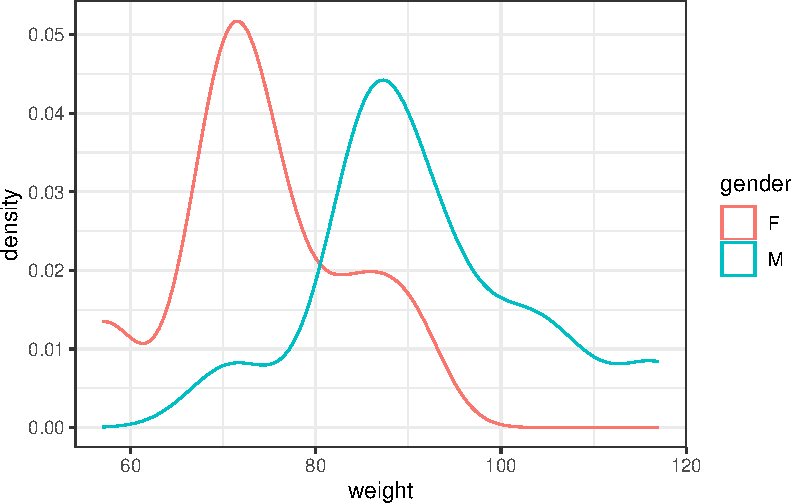
\includegraphics{경영통계분석_hw5_files/figure-pdf/unnamed-chunk-2-1.pdf}

여성, 남성별로 표본의 수, 표본평균, 표본표준편차는 아래와 같습니다.

\begin{Shaded}
\begin{Highlighting}[]
\NormalTok{weight }\SpecialCharTok{\%\textgreater{}\%}
  \FunctionTok{group\_by}\NormalTok{(gender) }\SpecialCharTok{\%\textgreater{}\%} 
  \FunctionTok{mutate}\NormalTok{(}\AttributeTok{cnt=}\DecValTok{1}\NormalTok{) }\SpecialCharTok{\%\textgreater{}\%} 
  \FunctionTok{summarise}\NormalTok{(}\AttributeTok{sample=}\FunctionTok{sum}\NormalTok{(cnt),}\AttributeTok{mean=}\FunctionTok{mean}\NormalTok{(weight),}\AttributeTok{vol=}\FunctionTok{sd}\NormalTok{(weight))}
\end{Highlighting}
\end{Shaded}

\begin{verbatim}
# A tibble: 2 x 4
  gender sample  mean   vol
  <chr>   <dbl> <dbl> <dbl>
1 F           8  73.9  10.1
2 M          11  91.9  12.4
\end{verbatim}

각 표본이 대략적으로 bell-shape를 형성하고 있으므로, 정규성 가정에 큰
무리는 없어보입니다.

따라서, 평균의 차이가 있는지 알아보기 위해서 t검정을 수행하겠습니다.

H0 : \(\mu_F=\mu_M\;\), H1 : \(\mu_F\neq\mu_M\)

\begin{Shaded}
\begin{Highlighting}[]
\FunctionTok{t.test}\NormalTok{(weight}\SpecialCharTok{\textasciitilde{}}\NormalTok{gender,}\AttributeTok{data=}\NormalTok{weight,}\AttributeTok{alternative=}\StringTok{"two.sided"}\NormalTok{,}\AttributeTok{paired=}\NormalTok{F)}
\end{Highlighting}
\end{Shaded}

\begin{verbatim}

    Welch Two Sample t-test

data:  weight by gender
t = -3.4971, df = 16.715, p-value = 0.002821
alternative hypothesis: true difference in means between group F and group M is not equal to 0
95 percent confidence interval:
 -28.928413  -7.139769
sample estimates:
mean in group F mean in group M 
       73.87500        91.90909 
\end{verbatim}

\textbf{p-value는 0.0028로 신뢰수준 5\% 하에서 귀무가설을 기각}할 수
있습니다.

\subsubsection*{(b)}\label{b-4}
\addcontentsline{toc}{subsubsection}{(b)}

모집단의 분포를 모르고 표본의 크기도 충분하지 않으므로, 표본평균의
정규성이 보장되지 않습니다.

또한, 두 집단의 평균 차이를 검정하기 위해서는 독립일 필요가 있으며,
t분포 유도를 위해 두 집단의 분산이 동일해야합니다.

따라서, \textbf{1. 임의추출(random samples), 2. 모집단의 정규성, 3. 두
모집단은 독립, 4. 두 모집단은 등분산}이라고 가정하였습니다.

\subsubsection*{(c)}\label{c-2}
\addcontentsline{toc}{subsubsection}{(c)}

두 집단의 분산이 같은지에 대해 검정하기 위해 분산차이에 대한 F검정을
수행하겠습니다.

H0 : \(\frac{\sigma_M}{\sigma_F}=1\;\), H1 :
\(\frac{\sigma_M}{\sigma_F}\neq 1\)

\begin{Shaded}
\begin{Highlighting}[]
\FunctionTok{var.test}\NormalTok{(weight}\SpecialCharTok{\textasciitilde{}}\NormalTok{gender,}\AttributeTok{data=}\NormalTok{weight)}
\end{Highlighting}
\end{Shaded}

\begin{verbatim}

    F test to compare two variances

data:  weight by gender
F = 0.66063, num df = 7, denom df = 10, p-value = 0.5981
alternative hypothesis: true ratio of variances is not equal to 1
95 percent confidence interval:
 0.1672544 3.1453141
sample estimates:
ratio of variances 
         0.6606253 
\end{verbatim}

P-value는 0.598로 귀무가설을 기각하지 못하였습니다. 이는 두 집단의
분산이 같다는 것을 지지하고 있습니다.

\subsubsection*{(d)}\label{d-1}
\addcontentsline{toc}{subsubsection}{(d)}

표본의 크기가 충분하지 않으므로 정규성이 담보되지 않아 F분포 및
카이제곱분포 유도를 위해 정규성 가정이 필요합니다.

또한, F분포 유도를 위해 두 집단이 독립일 필요가 있습니다.

따라서, \textbf{1. 임의추출(random samples), 2. 모집단의 정규성, 3. 두
모집단은 독립}이라고 가정하였습니다.



\end{document}
